%% Gabriel Madigan's PhD Thesis 
%% 19 October 2022

\documentclass[thesis]{neu}
%%% Packages included in thesis-umich class
%\RequirePackage[margin=1in,footskip=8pt,headsep=0.4cm,headheight=\baselineskip]{geometry}
%\RequirePackage{amsmath}
%\RequirePackage{amsfonts}
%\RequirePackage{amssymb}
%\RequirePackage{graphicx}
%\RequirePackage{subcaption}
%\RequirePackage{times}
%\RequirePackage{natbib}
%\RequirePackage{verbatim}
%\RequirePackage{upquote}
%\RequirePackage{textcomp}
%\RequirePackage{setspace}
%\RequirePackage{ifthen}
%\RequirePackage{soul}
%\RequirePackage{float}
%\RequirePackage[printonlyused]{acronym}
%\RequirePackage{makeidx}
%\RequirePackage{fancyhdr}
%\RequirePackage{multicol}
\usepackage{amsmath, amssymb}
\usepackage[ruled,vlined,linesnumbered]{algorithm2e}
\usepackage{etoolbox}
\AtBeginEnvironment{algorithm}{\setstretch{1.0}}
\usepackage[lofdepth=1]{subfig}
\usepackage[rightcaption]{sidecap}
\usepackage{multirow}
\usepackage{makecell}
\usepackage{url}
\usepackage{hyperref}
%\usepackage{natbib}
%\setcitestyle{square, numbers,sort&compress}
\usepackage{caption}
%\usepackage{subcaption} % Incompatable with subfig (line 25)
\usepackage{siunitx} % Provides the \SI{}{} and \si{} command for typesetting SI units
\usepackage{graphicx} % Required for the inclusion of images
\usepackage{titlesec}
\usepackage{braket}
\setcounter{secnumdepth}{4}
\usepackage[compat=1.0.0]{tikz-feynman}
%\usepackage[notocbib]{apacite}

% For inserting blank pages 
\usepackage{afterpage}
\newcommand\blankpage{%
    \null
    \thispagestyle{empty}%
    % \addtocounter{page}{-1}%
    \newpage}
    
    
% \usepackage{pdflscape}

% If you are using the alpha bibliography style, keep these next three lines in your preamble, so that the references are left-aligned; or, you can comment it out and see what happens
\makeatletter
\renewcommand{\@biblabel}[1]{[#1]\hfill}
\makeatother

\title{
A search for leptoquarks decaying to muons and bottom quarks in proton-proton collisions at \texorpdfstring{$\sqrt{s}=13$}{center-of-mass energies = 13} TeV with the full Run II data recorded by CMS 
}
 % \\ \newline 
% Author name
\author{Gabriel Madigan}

% Department
\department{Department of Physics} 

% Default style for front pages
\frontpagestyle{1} % 7 is preferred by Rackham, but should be set individually for each front page

% Acknowledgments (the input [7] determines the style -- 7 is Rackham's preferred style)
\acknowledgments{ 
    I would like to first thank my academic advisor, Emanuela Barberis, for guiding and supporting me through many years of research at Northeastern University and within the CMS collaboration. Ela is an exemplary physicist, and her direction of my academic research regularly challenged me to push myself as a scientist and academic.

I similarly would like to thank David Morse, who was a close collaborator on the Leptoquark analysis. His expertise on leptoquark searches, and his knowledge of our analysis framework, were indispensable in the completion of my disertation and progressing the analysis toward approval within the collaboration. Dave also oversaw the Phase-2 upgrades to the CSCs I participated in, helping me learn the ins-and-outs of the CSC system through hands-on detector work, as well as settling into the CSC group as a whole.

A special thank you to Tim Cox, the CSC DPG convener, who was a delight to work with. He took every opportunity to share his deep knowledge of the CSC conditions data with me (related to my role as contact to the AlCaDB group) and was always patient with me as I balanced my conditions-data-related workload with my physics analysis and CSC upgrade tasks. Furthermore, I would like to thank the whole CSC community, who warmly welcomed me into an exciting and unique chapter of my PhD while at CERN.

Also, a thank you to the CMS Exotica physics analysis group, for providing critical feedback on my physics analysis, ensuring that it stands up to the highest possible standards of scientific rigor.

To my fellow Northeastern/CMS collaborators and friends, Vivan, Abe, Yacine, Chad, Andrew, Tanvi, and Bingran; thank you for making my time in Boston and at CERN both a productive and enjoyable one, and for being the best travel companions on our many trips throughout Europe. And of course to my dear friends and fellow PhD candidates, Joam, Keegan, Ben, and everyone in my cohort at Northeastern, thank you for the academic support and camaraderie as we struggled through our first years of coursework and teaching, and for all the fun adventures we've had outside of academia as well; I will always cherish your friendship over these past seven years.

And last, but certainly not least, a heartfelt thank you to my family, Todd, Debbie, Natasha, Conor, and Henry. Without your support, guidance, and love, I know I would not be the man---or doctor---I am today. I love you all so much.
}

\abstract{
    


Many of the proposed extensions to the Standard Model of particle physics posit the existence of a new massive boson called a leptoquark that would couple directly to a quark and a lepton. Compelling evidence for new physics in flavor anomalies and the muon magnetic anomaly could indicate the involvement of these leptoquarks. High-energy proton-proton collisions at the Large Hadron Collider (LHC) are capable of producing leptoquark pairs---primarily through gluon-gluon fusion---providing LHC experiments like the Compact Muon Solenoid (CMS) collaboration with the perfect opportunity to look for these exotic particles. Presented in this thesis is a search for pair-produced scalar leptoquarks decaying to muons and bottom quarks, using \SI{138}{\invfb} of data collected by the CMS detector during the 2016--2018 proton-proton running of the LHC at a center-of-mass energy of \SI{13}{\TeV}. The final state event signature considered contains two high-transverse-momentum muons and two jets, one of which is tagged as originating from a bottom quark. This analysis is the first search for leptoquarks decaying to muons with the full LHC Run II dataset recorded by the CMS detector, as well as the first search by the CMS collaboration for leptoquarks in the \HepProcess{\Pmu\Pmu\Pbottom\text{j}} channel. Boosted decision trees were trained on the kinematics of the muons and jets in signal and background simulated data to select signal-like events for analysis. Observed and expected asymptotic upper limits were obtained at \SI{95}{\%} confidence level on the product of the signal production cross section and decay branching fraction into charged leptons as a function of the leptoquark mass. Comparison of these observed and expected limits with the theoretical cross sections establishes exclusion limits on leptoquark masses below \SI{1803}{\GeV} and \SI{1796}{\GeV}, respectively. The results of this study mark the strongest limits to date on leptoquarks decaying to muons and bottom quarks.
}

\hidepreface

% Committee
\committee{ %
Professor Emanuela Barberis, Chair \\
Professor James Halverson \\
Professor Toyoko Orimoto \\
Professor Darien Wood
}

% Chair must be entered separately for formatting reasons.
\chair{Professor Emanuela Barberis}

%%-- Begin Document
\begin{document}
% \maketitle
% \doublespacing
% \tableofcontents
% \singlespacing % if you want single spacing after showing the table of contents
\newpage 

% ref: https://gitlab.cern.ch/tdr/utils/-/blob/master/general/ptdr-definitions.sty

\newcommand{\Htogg}{$\mathrm{H}\to\gamma\gamma$\xspace}
\newcommand{\Ztoee}{$\mathrm{Z}\to\mathrm{e}^{+}\mathrm{e}^{-}$\xspace}
\newcommand{\Ztommg}{$\mathrm{Z}\to\mu^{+}\mu^{-}\gamma$\xspace}

\newcommand{\ptgg}{$\pt^{\gamma\gamma}$\xspace}
\newcommand{\mgg}{\ensuremath{m_{\gamma\gamma}}\xspace}

% \newcommand{\ptvecmiss}{\ensuremath{{\vec p}_{\mathrm{T}}^{\kern1pt\text{miss}}}\xspace}
% \newcommand{\pt}{\ensuremath{p_{\mathrm{T}}}\xspace}
% \newcommand{\ptmiss}{\ensuremath{\pt^\text{miss}}\xspace}

% \DeclareRobustCommand{\PH}{{\HepParticle{H}{}{}}\Xspace} % standard/heavy Higgs

\newcommand{\PH}{H}

% Some software programs (alphabetized)
\newcommand{\ACERMC} {\textsc{AcerMC}\xspace}
\newcommand{\ALPGEN} {{\textsc{alpgen}}\xspace}
\newcommand{\BLACKHAT} {{\textsc{BlackHat}}\xspace}
\newcommand{\CALCHEP} {{\textsc{CalcHEP}}\xspace}
\newcommand{\CHARYBDIS} {{\textsc{charybdis}}\xspace}
\newcommand{\CMKIN} {\textsc{cmkin}\xspace}
\newcommand{\CMSIM} {{\textsc{cmsim}}\xspace}
\newcommand{\CMSSW} {{\textsc{cmssw}}\xspace}
\newcommand{\COBRA} {{\textsc{cobra}}\xspace}
\newcommand{\COCOA} {{\textsc{cocoa}}\xspace}
\newcommand{\COMPHEP} {\textsc{CompHEP}\xspace}
\newcommand{\EVTGEN} {{\textsc{evtgen}}\xspace}
\newcommand{\FAMOS} {{\textsc{famos}}\xspace}
\newcommand{\FASTJET} {{\textsc{FastJet}}\xspace}
\newcommand{\FEWZ} {{\textsc{fewz}}\xspace}
\newcommand{\GARCON} {\textsc{garcon}\xspace}
\newcommand{\GARFIELD} {{\textsc{garfield}}\xspace}
\newcommand{\GEANE} {{\textsc{geane}}\xspace}
\newcommand{\GEANTfour} {{\textsc{Geant4}}\xspace}
\newcommand{\GEANTthree} {{\textsc{geant3}}\xspace}
\newcommand{\GEANT} {{\textsc{geant}}\xspace}
\newcommand{\HDECAY} {\textsc{hdecay}\xspace}
\newcommand{\HERWIG} {{\textsc{herwig}}\xspace}
\newcommand{\HERWIGpp} {{\textsc{herwig++}}\xspace}
\newcommand{\POWHEG} {{\textsc{powheg}}\xspace}
\newcommand{\HIGLU} {{\textsc{higlu}}\xspace}
\newcommand{\HIJING} {{\textsc{hijing}}\xspace}
\newcommand{\HYDJET} {{\textsc{hydjet}}\xspace}
\newcommand{\IGUANA} {\textsc{iguana}\xspace}
\newcommand{\ISAJET} {{\textsc{isajet}}\xspace}
\newcommand{\ISAPYTHIA} {{\textsc{isapythia}}\xspace}
\newcommand{\ISASUGRA} {{\textsc{isasugra}}\xspace}
\newcommand{\ISASUSY} {{\textsc{isasusy}}\xspace}
\newcommand{\ISAWIG} {{\textsc{isawig}}\xspace}
\newcommand{\MADGRAPH} {\textsc{MadGraph}\xspace}
\newcommand{\MCATNLO} {\textsc{mc@nlo}\xspace}
\newcommand{\MCFM} {\textsc{mcfm}\xspace}
\newcommand{\MILLEPEDE} {{\textsc{millepede}}\xspace}
\newcommand{\ORCA} {{\textsc{orca}}\xspace}
\newcommand{\OSCAR} {{\textsc{oscar}}\xspace}
% \newcommand{\PHOTOS} {\textsc{photos}\xspace}
\newcommand{\PROSPINO} {\textsc{prospino}\xspace}
\newcommand{\PYTHIA} {{\textsc{pythia}}\xspace}
\newcommand{\SHERPA} {{\textsc{sherpa}}\xspace}
\newcommand{\TAUOLA} {\textsc{tauola}\xspace}
\newcommand{\TOPREX} {\textsc{TopReX}\xspace}
\newcommand{\XDAQ} {{\textsc{xdaq}}\xspace}
\newcommand{\MGvATNLO}{\MADGRAPH{}5\_a\MCATNLO}
\newcommand{\TOPpp}{\textsc{Top++}\xspace}
\newcommand{\GENEVA}{\textsc{geneva}\xspace}

%  Experiments
\newcommand {\DZERO}{D0\xspace}     %etc.


% Measurements and units...

\newcommand{\de}{\ensuremath{^\circ}}
\newcommand{\ten}[1]{\ensuremath{\times \text{10}^\text{#1}}}
\newcommand{\unit}[1]{\ensuremath{\text{\,#1}}\xspace}
\newcommand{\mum}{\ensuremath{\,\mu\text{m}}\xspace}
\newcommand{\micron}{\ensuremath{\,\mu\text{m}}\xspace}
\renewcommand{\cm}{\ensuremath{\,\text{cm}}\xspace}
\renewcommand{\mm}{\ensuremath{\,\text{mm}}\xspace}
\newcommand{\mus}{\ensuremath{\,\mu\text{s}}\xspace}
\renewcommand{\keV}{\ensuremath{\,\text{ke\hspace{-.08em}V}}\xspace}
\renewcommand{\MeV}{\ensuremath{\,\text{Me\hspace{-.08em}V}}\xspace}
\newcommand{\MeVns}{\ensuremath{\text{Me\hspace{-.08em}V}}\xspace} % no leading thinspace
\renewcommand{\GeV}{\ensuremath{\,\text{Ge\hspace{-.08em}V}}\xspace}
\newcommand{\GeVns}{\ensuremath{\text{Ge\hspace{-.08em}V}}\xspace} % no leading thinspace
\newcommand{\gev}{\GeV}
\renewcommand{\TeV}{\ensuremath{\,\text{Te\hspace{-.08em}V}}\xspace}
\newcommand{\TeVns}{\ensuremath{\text{Te\hspace{-.08em}V}}\xspace} % no leading thinspace
\newcommand{\PeV}{\ensuremath{\,\text{Pe\hspace{-.08em}V}}\xspace}
\newcommand{\keVc}{\ensuremath{{\,\text{ke\hspace{-.08em}V\hspace{-0.16em}/\hspace{-0.08em}}c}}\xspace}
\newcommand{\MeVc}{\ensuremath{{\,\text{Me\hspace{-.08em}V\hspace{-0.16em}/\hspace{-0.08em}}c}}\xspace}
\newcommand{\GeVc}{\ensuremath{{\,\text{Ge\hspace{-.08em}V\hspace{-0.16em}/\hspace{-0.08em}}c}}\xspace}
\newcommand{\GeVcns}{\ensuremath{{\text{Ge\hspace{-.08em}V\hspace{-0.16em}/\hspace{-0.08em}}c}}\xspace} % no leading thinspace
\newcommand{\TeVc}{\ensuremath{{\,\text{Te\hspace{-.08em}V\hspace{-0.16em}/\hspace{-0.08em}}c}}\xspace}
\newcommand{\keVcc}{\ensuremath{{\,\text{ke\hspace{-.08em}V\hspace{-0.16em}/\hspace{-0.08em}}c^\text{2}}}\xspace}
\newcommand{\MeVcc}{\ensuremath{{\,\text{Me\hspace{-.08em}V\hspace{-0.16em}/\hspace{-0.08em}}c^\text{2}}}\xspace}
\newcommand{\GeVcc}{\ensuremath{{\,\text{Ge\hspace{-.08em}V\hspace{-0.16em}/\hspace{-0.08em}}c^\text{2}}}\xspace}
\newcommand{\GeVccns}{\ensuremath{{\text{Ge\hspace{-.08em}V\hspace{-0.16em}/\hspace{-0.08em}}c^\text{2}}}\xspace} % no leading thinspace
\newcommand{\TeVcc}{\ensuremath{{\,\text{Te\hspace{-.08em}V\hspace{-0.16em}/\hspace{-0.08em}}c^\text{2}}}\xspace}

\newcommand{\abinv} {\mbox{\ensuremath{\,\text{ab}^{-1}}}\xspace}
\newcommand{\fbinv} {\mbox{\ensuremath{\,\text{fb}^{-1}}}\xspace}
\newcommand{\pbinv} {\mbox{\ensuremath{\,\text{pb}^{-1}}}\xspace}
\newcommand{\nbinv} {\mbox{\ensuremath{\,\text{nb}^{-1}}}\xspace}
\newcommand{\mubinv} {\ensuremath{\,\mu\text{b}^{-1}}\xspace}
\newcommand{\mbinv} {\ensuremath{\,\text{mb}^{-1}}\xspace}
\newcommand{\percms}{\ensuremath{\,\text{cm}^{-2}\,\text{s}^{-1}}\xspace}
\newcommand{\lumi}{\ensuremath{\mathcal{L}}\xspace}
\newcommand{\Lumi}{\ensuremath{\mathcal{L}}\xspace}%both upper and lower
%
% Need a convention here:
\newcommand{\LvLow}  {\ensuremath{\mathcal{L}=\text{10}^\text{32}\,\text{cm}^\text{$-$2}\,\text{s}^\text{$-$1}}\xspace}
\newcommand{\LLow}   {\ensuremath{\mathcal{L}=\text{10}^\text{33}\,\text{cm}^\text{$-$2}\,\text{s}^\text{$-$1}}\xspace}
\newcommand{\lowlumi}{\ensuremath{\mathcal{L}=\text{2}\times \text{10}^\text{33}\,\text{cm}^\text{$-$2}\,\text{s}^\text{$-$1}}\xspace}
\newcommand{\LMed}   {\ensuremath{\mathcal{L}=\text{2}\times \text{10}^\text{33}\,\text{cm}^\text{$-$2}\,\text{s}^\text{$-$1}}\xspace}
\newcommand{\LHigh}  {\ensuremath{\mathcal{L}=\text{10}^\text{34}\,\text{cm}^\text{$-$2}\,\text{s}^\text{$-$1}}\xspace}
\newcommand{\hilumi} {\ensuremath{\mathcal{L}=\text{10}^\text{34}\,\text{cm}^\text{$-$2}\,\text{s}^\text{$-$1}}\xspace}

% Physics symbols ...

\newcommand{\PT}{\ensuremath{p_{\mathrm{T}}}\xspace}
\newcommand{\pt}{\ensuremath{p_{\mathrm{T}}}\xspace}
\newcommand{\ET}{\ensuremath{E_{\mathrm{T}}}\xspace}
\newcommand{\HT}{\ensuremath{H_{\mathrm{T}}}\xspace}
\newcommand{\mT}{\ensuremath{m_{\mathrm{T}}}\xspace}
\newcommand{\mTii}{\ensuremath{m_{\mathrm{T2}}}\xspace}
\newcommand{\et}{\ensuremath{E_{\mathrm{T}}}\xspace}
\newcommand{\Em}{\ensuremath{E\hspace{-0.6em}/}\xspace}
\newcommand{\Pm}{\ensuremath{p\hspace{-0.5em}/}\xspace}
\newcommand{\PTm}{\ensuremath{{p}_\mathrm{T}\hspace{-1.02em}/\kern 0.5em}\xspace}
\newcommand{\PTslash}{\PTm}
\newcommand{\ETm}{\ensuremath{E_{\mathrm{T}}^{\text{miss}}}\xspace}
\newcommand{\MET}{\ETm}
\newcommand{\ETmiss}{\ETm}
\newcommand{\ptmiss}{\ensuremath{\pt^\text{miss}}\xspace}
\newcommand{\ETslash}{\ensuremath{E_{\mathrm{T}}\hspace{-1.1em}/\kern0.45em}\xspace}
\newcommand{\VEtmiss}{\ensuremath{{\vec E}_{\mathrm{T}}^{\text{miss}}}\xspace}
\newcommand{\ptvec}{\ensuremath{{\vec p}_{\mathrm{T}}}\xspace}
\newcommand{\ptvecmiss}{\ensuremath{{\vec p}_{\mathrm{T}}^{\kern1pt\text{miss}}}\xspace}
\newcommand{\tauh}{\ensuremath{\PGt_\mathrm{h}}\xspace}
\newcommand{\sqrtsNN}{\ensuremath{\sqrt{\smash[b]{s_{_{\mathrm{NN}}}}}}\xspace}
\newcommand{\mht}{\ensuremath{H_{\mathrm{T}}^{\text{miss}}}\xspace}
\newcommand{\htvecmiss}{\ensuremath{\vec{H}_{\text{T}}^{\text{miss}}}\xspace}

% roman face derivative
\newcommand{\dd}[2]{\ensuremath{\frac{\cmsSymbolFace{d} #1}{\cmsSymbolFace{d} #2}}}
\newcommand{\ddinline}[2]{\ensuremath{\cmsSymbolFace{d} #1/\cmsSymbolFace{d} #2}}
\newcommand{\rd}{\ensuremath{\cmsSymbolFace{d}}}
\newcommand{\re}{\ensuremath{\cmsSymbolFace{e}}}
% absolute value
\newcommand{\abs}[1]{\ensuremath{\lvert #1 \rvert}}
% misc
\newcommand{\CL}{\ensuremath{\text{CL}}\xspace} % needs to be overridden to C.L. for APS. Look out for \CL.
\newcommand{\CLs}{\ensuremath{\text{CL}_\text{s}}\xspace}
\newcommand{\CLsb}{\ensuremath{\text{CL}_\text{s+b}}\xspace}


% Particle names which track the italic/non-italic face convention
\newcommand{\zp}{{\PZpr}\xspace} % plain Z'
\newcommand{\JPsi}{{\PJGy}\xspace} % J/Psi (no mass)
\newcommand{\Z}{{\PZ}\xspace} % plain Z (no superscript 0)
\newcommand{\ttbar}{{\PQt{}\PAQt}\xspace} % t-tbar

% Extensions for missing names in PENNAMES % note now has xspace, to match syntax in PENNAMES2
\newcommand{\cPgn}{\PGn} % generic neutrino
\providecommand{\Pgn}{\PGn}
\newcommand{\cPagn}{\PAGn} % generic anti-neutrino
\providecommand{\Pagn}{\PAGn}
\newcommand{\cPgg}{\PGg} % gamma
\newcommand{\cPJgy}{\PJGy} % J/Psi (no mass)
\newcommand{\cPZ}{\PZ} % plain Z (no superscript 0)
\newcommand{\cPZpr}{\PZpr} % plain Z'
\newcommand{\cPqt}{\PQt} % t for t quark
\newcommand{\cPqb}{\PQb} % b for b quark
\newcommand{\cPqc}{\PQc} % c for c quark
\newcommand{\cPqs}{\PQs} % s for s quark
\newcommand{\cPqu}{\PQu} % u for u quark
\newcommand{\cPqd}{\PQd} % d for d quark
\newcommand{\cPq}{\PQq} % generic quark
\newcommand{\cPg}{\Pg} % generic gluon
\newcommand{\cPG}{\PXXG} % Graviton
\newcommand{\cPaqt}{\PAQt} % t for t anti-quark
\newcommand{\cPaqb}{\PAQb} % b for b anti-quark
\newcommand{\cPaqc}{\PAQc} % c for c anti-quark
\newcommand{\cPaqs}{\PAQs} % s for s anti-quark
\newcommand{\cPaqu}{\PAQu} % u for u anti-quark
\newcommand{\cPaqd}{\PAQd} % d for d anti-quark
\newcommand{\cPaq}{\PAQq} % generic anti-quark
\newcommand{\cPKstz}{\ensuremath{\PK^{\ast0}}\xspace}
% in-between: ought to be in heppennames2, but isn't
\newcommand{\PQT}{{\HepParticle{T}{}{}}\Xspace}
\newcommand{\PQB}{{\HepParticle{B}{}{}}\Xspace}
% our extensions for pennames2
\providecommand{\Pepm}{\ensuremath{\Pe^\pm}\xspace}
\providecommand{\Pemp}{\ensuremath{\Pe^\mp}\xspace}
\providecommand{\PGmpm}{\ensuremath{\PGm^\pm}\xspace}
\providecommand{\PGmmp}{\ensuremath{\PGm^\mp}\xspace} % not available in pennames2, AFAIK
\providecommand{\PGUPnS}{\PGUP{nS}\xspace}% maps to \PGUP[nS]
\providecommand{\PV}{{\HepParticle{V}{}{}}\Xspace} % generic vector boson
\providecommand{\Pell}{\HepParticle{\ell}{}{}\Xspace} % generic lepton (like \Pl, but using \ell)
\providecommand{\PQQ}{\HepParticle{Q}{}{}\Xspace} % generic heavy quark
\providecommand{\PAQQ}{\HepAntiParticle{Q}{}{}\Xspace} % generic heavy antiquark

% Other
\newcommand{\MD}{\ensuremath{{M_\mathrm{D}}}\xspace}% ED mass
\newcommand{\Mpl}{\ensuremath{{M_\mathrm{Pl}}}\xspace}% Planck mass
\newcommand{\Rinv} {\ensuremath{{R}^{-1}}\xspace}

% SM (still to be classified)

\newcommand{\AFB}{\ensuremath{A_\text{FB}}\xspace}
\newcommand{\wangle}{\ensuremath{\sin^{2}\theta_{\text{eff}}^\text{lept}(M^2_{\Z})}\xspace}
\newcommand{\stat}{\ensuremath{\,\text{(stat)}}\xspace}
\newcommand{\syst}{\ensuremath{\,\text{(syst)}}\xspace}
\newcommand{\thy}{\ensuremath{\,\text{(theo)}}\xspace}
\newcommand{\lum}{\ensuremath{\,\text{(lumi)}}\xspace}
\newcommand{\kt}{\ensuremath{k_{\mathrm{T}}}\xspace}

\newcommand{\BC}{\HepParticle{B}{c}{}{}\xspace}
\newcommand{\bbarc}{\PAQb{}\PQc\xspace}
\newcommand{\bbbar}{\PQb{}\PAQb\xspace}
\newcommand{\ccbar}{\PQc{}\PAQc\xspace}
\newcommand{\qqbar}{\ensuremath{\PQq\PAQq}\xspace}
\newcommand{\bspsiphi}{\ensuremath{\PBs \to \JPsi\, \PGf}\xspace}
\newcommand{\EE}{\Pep{}\Pem\xspace}
\newcommand{\MM}{\PGmp{}\PGmm\xspace}
\newcommand{\TT}{\PGtm{}\PGtp\xspace}

%%%  E-gamma definitions
% \newcommand{\HGG}{\ensuremath{\PH\to\PGg\PGg}}
\newcommand{\GAMJET}{\ensuremath{\PGg + \text{jet}}}
\newcommand{\PPTOJETS}{\ensuremath{\Pp\Pp\to\text{jets}}}
\newcommand{\PPTOGG}{\ensuremath{\Pp\Pp\to\PGg\PGg}}
\newcommand{\PPTOGAMJET}{\ensuremath{\Pp\Pp\to\PGg + \text{jet}}}
% \newcommand{\MH}{\ensuremath{M_{\PH}}}
\newcommand{\RNINE}{\ensuremath{R_\mathrm{9}}}
\newcommand{\DR}{\ensuremath{\Delta R}}





%%%%%%
% From Albert De Roeck for original TDRs
%

\newcommand{\ga}{\ensuremath{\gtrsim}}
\newcommand{\la}{\ensuremath{\lesssim}}
%
\newcommand{\swsq}{\ensuremath{\sin^2\theta_{\PW}}\xspace}
\newcommand{\cwsq}{\ensuremath{\cos^2\theta_{\PW}}\xspace}
\newcommand{\tanb}{\ensuremath{\tan\beta}\xspace}
\newcommand{\tanbsq}{\ensuremath{\tan^{2}\beta}\xspace}
\newcommand{\sidb}{\ensuremath{\sin 2\beta}\xspace}
\newcommand{\alpS}{\ensuremath{\alpha_\mathrm{S}}\xspace}
\newcommand{\alpt}{\ensuremath{\tilde{\alpha}}\xspace}

\newcommand{\QL}{\HepParticle{Q}{L}{}{}\xspace}
\newcommand{\sQ}{\HepSusyParticle{Q}{}{}{}\xspace}
\newcommand{\sQL}{\HepSusyParticle{Q}{L}{}{}\xspace}
\newcommand{\ULC}{\HepParticle{U}{L}{C}{}\xspace}
\newcommand{\sUC}{\HepSusyParticle{U}{}{C}{}\xspace}
\newcommand{\sULC}{\HepSusyParticle{U}{L}{C}{}\xspace}
\newcommand{\DLC}{\HepParticle{D}{L}{C}{}\xspace}
\newcommand{\sDC}{\HepSusyParticle{D}{}{C}{}\xspace}
\newcommand{\sDLC}{\HepSusyParticle{D}{L}{C}{}\xspace}
\newcommand{\LL}{\HepParticle{L}{L}{}{}\xspace}
\newcommand{\sL}{\HepSusyParticle{L}{}{}{}\xspace}
\newcommand{\sLL}{\HepSusyParticle{L}{L}{}{}\xspace}
\newcommand{\ELC}{\HepParticle{E}{L}{C}{}\xspace}
\newcommand{\sEC}{\HepSusyParticle{E}{}{C}{}\xspace}
\newcommand{\sELC}{\HepSusyParticle{E}{L}{C}{}\xspace}
\newcommand{\sEL}{\HepSusyParticle{E}{L}{}{}\xspace}
\newcommand{\sER}{\HepSusyParticle{E}{R}{}{}\xspace}
\newcommand{\sFer}{\HepSusyParticle{f}{}{}{}\xspace}
\newcommand{\sQua}{\PSQ}
\newcommand{\sUp}{\PSQu}
\newcommand{\suL}{\PSQuL}
\newcommand{\suR}{\PSQuR}
\newcommand{\sDw}{\PSQd}
\newcommand{\sdL}{\PSQdL}
\newcommand{\sdR}{\PSQdR}
\newcommand{\sTop}{\PSQt}
\newcommand{\stL}{\PSQtL}
\newcommand{\stR}{\PSQtR}
\newcommand{\stone}{\PSQtDo}
\newcommand{\sttwo}{\PSQtDt}
\newcommand{\sBot}{\PSQb}
\newcommand{\sbL}{\PSQbL}
\newcommand{\sbR}{\PSQbR}
\newcommand{\sbone}{\PSQbDo}
\newcommand{\sbtwo}{\PSQbDt}
\newcommand{\sLep}{\PSl}
\newcommand{\sLepC}{\HepSusyParticle{l}{}{C}{}\xspace}
\newcommand{\sEl}{\PSe}
\newcommand{\sElC}{\HepSusyParticle{e}{}{C}{}\xspace}
\newcommand{\seL}{\PSeL}
\newcommand{\seR}{\PSeR}
\newcommand{\snL}{\HepSusyParticle{\PGn}{L}{}{}\xspace}
\newcommand{\sMu}{\PSGm}
\newcommand{\sNu}{\PSGn}
\newcommand{\sTau}{\PSGt}
\newcommand{\Glu}{\Pg}
\newcommand{\sGlu}{\PSg}
\newcommand{\Wpm}{\PWpm}
\newcommand{\sWpm}{\PSWpm}
\newcommand{\Wz}{\HepParticle{W}{}{0}{}\xspace}
\newcommand{\sWz}{\HepSusyParticle{W}{}{0}{}\xspace}
\newcommand{\sWino}{\PSW}
\newcommand{\Bz}{\HepParticle{B}{}{0}\xspace}
\newcommand{\sBz}{\HepSusyParticle{B}{}{0}\xspace}
\newcommand{\sBino}{\HepSusyParticle{B}{}{}\xspace}
\newcommand{\Zz}{\PZz}
\newcommand{\sZino}{\PSZz}
\newcommand{\sGam}{\PSGg}
\newcommand{\chiz}{\PSGcz}
\newcommand{\chip}{\PSGcp}
\newcommand{\chim}{\PSGcm}
\newcommand{\chipm}{\PSGcpm}
\newcommand{\Hone}{\HepParticle{H}{d}{}\xspace}
\newcommand{\sHone}{\HepSusyParticle{H}{d}{}\xspace}
\newcommand{\Htwo}{\HepParticle{H}{u}{}\xspace}
\newcommand{\sHtwo}{\HepSusyParticle{H}{u}{}\xspace}
\newcommand{\sHig}{\HepSusyParticle{H}{}{}{}\xspace}
\newcommand{\sHa}{\HepSusyParticle{H}{a}{}{}\xspace}
\newcommand{\sHb}{\HepSusyParticle{H}{b}{}{}\xspace}
\newcommand{\sHpm}{\HepSusyParticle{H}{}{\pm}{}\xspace}
\newcommand{\hz}{\PShz}
% \newcommand{\Hz}{\PHz}
\newcommand{\Az}{\PSAz}
\newcommand{\Hpm}{\PSHpm}
\newcommand{\sGra}{\PXXSG}
%
\newcommand{\mtil}{\ensuremath{\widetilde{m}}\xspace}
%
\newcommand{\rpv}{\ensuremath{\rlap{\kern.2em/}R}\xspace}
\newcommand{\LLE}{\ensuremath{LL\bar{E}}\xspace}
\newcommand{\LQD}{\ensuremath{LQ\bar{D}}\xspace}
\newcommand{\UDD}{\ensuremath{\overline{UDD}}\xspace}
\newcommand{\Lam}{\ensuremath{\lambda}\xspace}
\newcommand{\Lamp}{\ensuremath{\lambda'}\xspace}
\newcommand{\Lampp}{\ensuremath{\lambda''}\xspace}
%
\newcommand{\spinbd}[2]{\ensuremath{\bar{#1}_{\dot{#2}}}\xspace}

%pennames to heppenames2 translation
%no longer include mass
%PDstpm
%PKst
%
%no j subscript, no tilde
%PSHpm
%PSHz
%
%Added overbar
%PagXz
%
%Removed overbar
%PgXz
%
\newcommand{\PAz}{\PSAz}
\newcommand{\PDiz}{\PDzDoP{2420}}
\newcommand{\PDstiiz}{\PDstzDtP{2460}}
\newcommand{\PDstz}{\PDstzP{2010}}
% \newcommand{\PHpm}{\PSHpm}
\newcommand{\PJgy}{\PJGyP{1S}}
\newcommand{\PKia}{\PKDoP{1400}}
\newcommand{\PKii}{\PKDtP{1770}}
\newcommand{\PKi}{\PKDoP{1270}}
\newcommand{\PKsta}{\PKstP{1370}}
\newcommand{\PKstb}{\PKstP{1680}}
\newcommand{\PKstiii}{\PKstDTP{1780}}
\newcommand{\PKstii}{\PKstDtP{1430}}
\newcommand{\PKstiv}{\PKstDfP{2045}}
\newcommand{\PKstz}{\PKstDzP{1430}}
\newcommand{\PNa}{\HepParticleResonanceFormalFull{\PN}{}{}{1440}{}{}{P}{11}{}\xspace}
\newcommand{\PNb}{\HepParticleResonanceFormalFull{\PN}{}{}{1520}{}{}{D}{13}{}\xspace}
\newcommand{\PNc}{\HepParticleResonanceFormalFull{\PN}{}{}{1535}{}{}{S}{11}{}\xspace}
\newcommand{\PNd}{\HepParticleResonanceFormalFull{\PN}{}{}{1650}{}{}{S}{11}{}\xspace}
\newcommand{\PNe}{\HepParticleResonanceFormalFull{\PN}{}{}{1675}{}{}{D}{15}{}\xspace}
\newcommand{\PNf}{\HepParticleResonanceFormalFull{\PN}{}{}{1680}{}{}{F}{15}{}\xspace}
\newcommand{\PNg}{\HepParticleResonanceFormalFull{\PN}{}{}{1700}{}{}{D}{13}{}\xspace}
\newcommand{\PNh}{\HepParticleResonanceFormalFull{\PN}{}{}{1710}{}{}{P}{11}{}\xspace}
\newcommand{\PNi}{\HepParticleResonanceFormalFull{\PN}{}{}{1720}{}{}{P}{13}{}\xspace}
\newcommand{\PNj}{\HepParticleResonanceFormalFull{\PN}{}{}{2190}{}{}{G}{17}{}\xspace}
\newcommand{\PNk}{\HepParticleResonanceFormalFull{\PN}{}{}{2220}{}{}{H}{19}{}\xspace}
\newcommand{\PNl}{\HepParticleResonanceFormalFull{\PN}{}{}{2250}{}{}{G}{19}{}\xspace}
\newcommand{\PNm}{\HepParticleResonanceFormalFull{\PN}{}{}{2600}{}{}{I}{1,11}{}\xspace}
\newcommand{\PSHz}{\HepParticle{\PSH}{}{0}{}}
\newcommand{\PSgg}{\PSGg}
\newcommand{\PSgm}{\PSGm}
\newcommand{\PSgn}{\PSGn}
\newcommand{\PSgt}{\PSGt}
\newcommand{\PSgxpm}{\PSGcpm}
\newcommand{\PSgxz}{\PSGcz}
\newcommand{\PSq}{\PSQ}
\newcommand{\PZgc}{\PZGc}
\newcommand{\PZge}{\PZGe}
\newcommand{\PZgy}{\PZGy}
\newcommand{\PZi}{\HepParticle{Z}{1}{}\xspace}
\newcommand{\PaBz}{\PABz}
\newcommand{\PaB}{\PAB}
\newcommand{\PaDz}{\PADz}
\newcommand{\PaD}{\PAD}
\newcommand{\PaKz}{\PAKz}
\newcommand{\PaSq}{\PASQ}
\newcommand{\PagL}{\PAGL}
\newcommand{\PagOp}{\HepAntiParticle{\PGO}{}{+}\xspace}
\newcommand{\PagSm}{\HepAntiParticle{\PGS}{}{-}\xspace}
\newcommand{\PagSp}{\HepAntiParticle{\PGS}{}{+}\xspace}
\newcommand{\PagSz}{\HepAntiParticle{\PGS}{}{0}\xspace}
\newcommand{\PagXp}{\HepAntiParticle{\PGX}{}{+}\xspace}
\newcommand{\PagXz}{\HepAntiParticle{\PGX}{}{0}\xspace}
\newcommand{\Pagne}{\PAGne}
\newcommand{\Pagngm}{\PAGnGm}
\newcommand{\Pagngt}{\PAGnGt}
\newcommand{\Paii}{\PaDtP{1320}}
\newcommand{\Pai}{\PaDoP{1260}}
\newcommand{\Pap}{\PAp}
\newcommand{\Paqb}{\PAQqb}
\newcommand{\Paqc}{\PAQqc}
\newcommand{\Paqd}{\PAQqd}
\newcommand{\Paqs}{\PAQqs}
\newcommand{\Paqt}{\PAQqt}
\newcommand{\Paqu}{\PAQqu}
\newcommand{\Paq}{\PAQq}
\newcommand{\Paz}{\PaDzP{980}}
\newcommand{\Pbgcia}{\PGcbDoP{2P}}
\newcommand{\Pbgciia}{\PGcbDtP{2P}}
\newcommand{\Pbgcii}{\PGcbDtP{1P}}
\newcommand{\Pbgci}{\PGcbDoP{1P}}
\newcommand{\Pbgcza}{\PGcbDzP{2P}}
\newcommand{\Pbgcz}{\PGcbDzP{1P}}
\newcommand{\Pbi}{\PbDoP{1235}}
\newcommand{\PcgLp}{\PGLpc}
\newcommand{\PcgS}{\PGScP{2455}}
\newcommand{\PcgXp}{\PGXpc}
\newcommand{\PcgXz}{\PGXzc}
\newcommand{\Pcgcii}{\PGccDtP{1P}}
\newcommand{\Pcgci}{\PGccDoP{1P}}
\newcommand{\Pcgcz}{\PGccDzP{1S}}
\newcommand{\Pcgh}{\PGhcP{1S}}
\newcommand{\Pfia}{\PfDoP{1390}}
\newcommand{\Pfib}{\PfDoP{1510}}
\newcommand{\Pfiia}{\PfDtP{1720}}
\newcommand{\Pfiib}{\PfDtP{2010}}
\newcommand{\Pfiic}{\PfDtP{2300}}
\newcommand{\Pfiid}{\PfDtP{2340}}
\newcommand{\Pfiipr}{\PfprDtP{1525}}
\newcommand{\Pfii}{\PfDtP{1270}}
\newcommand{\Pfiv}{\PfDfP{2050}}
\newcommand{\Pfi}{\PfDoP{1285}}
\newcommand{\Pfza}{\PfDzP{1400}}
\newcommand{\Pfzb}{\PfDzP{1590}}
\newcommand{\Pfz}{\PfDzP{975}}
\newcommand{\PgD}{\PGD}
\newcommand{\PgDa}{\HepParticleResonanceFormalFull{\PGD}{}{}{1232}{}{}{P}{33}{}\xspace}
\newcommand{\PgDb}{\HepParticleResonanceFormalFull{\PGD}{}{}{1620}{}{}{S}{31}{}\xspace}
\newcommand{\PgDc}{\HepParticleResonanceFormalFull{\PGD}{}{}{1700}{}{}{D}{33}{}\xspace}
\newcommand{\PgDd}{\HepParticleResonanceFormalFull{\PGD}{}{}{1900}{}{}{S}{31}{}\xspace}
\newcommand{\PgDe}{\HepParticleResonanceFormalFull{\PGD}{}{}{1905}{}{}{F}{35}{}\xspace}
\newcommand{\PgDf}{\HepParticleResonanceFormalFull{\PGD}{}{}{1910}{}{}{P}{31}{}\xspace}
\newcommand{\PgDh}{\HepParticleResonanceFormalFull{\PGD}{}{}{1920}{}{}{P}{33}{}\xspace}
\newcommand{\PgDi}{\HepParticleResonanceFormalFull{\PGD}{}{}{1930}{}{}{D}{35}{}\xspace}
\newcommand{\PgDj}{\HepParticleResonanceFormalFull{\PGD}{}{}{1950}{}{}{F}{37}{}\xspace}
\newcommand{\PgDk}{\HepParticleResonanceFormalFull{\PGD}{}{}{2420}{}{}{H}{3,11}{}\xspace}
\newcommand{\PgL}{\PGL}
\newcommand{\PgLa}{\HepParticleResonanceFormalFull{\PGL}{}{}{1405}{}{}{S}{01}{}}
\newcommand{\PgLb}{\HepParticleResonanceFormalFull{\PGL}{}{}{1520}{}{}{D}{03}{}}
\newcommand{\PgLc}{\HepParticleResonanceFormalFull{\PGL}{}{}{1600}{}{}{P}{01}{}}
\newcommand{\PgLd}{\HepParticleResonanceFormalFull{\PGL}{}{}{1670}{}{}{S}{01}{}}
\newcommand{\PgLe}{\HepParticleResonanceFormalFull{\PGL}{}{}{1690}{}{}{D}{03}{}}
\newcommand{\PgLf}{\HepParticleResonanceFormalFull{\PGL}{}{}{1800}{}{}{S}{01}{}}
\newcommand{\PgLg}{\HepParticleResonanceFormalFull{\PGL}{}{}{1810}{}{}{P}{01}{}}
\newcommand{\PgLh}{\HepParticleResonanceFormalFull{\PGL}{}{}{1820}{}{}{F}{05}{}}
\newcommand{\PgLi}{\HepParticleResonanceFormalFull{\PGL}{}{}{1830}{}{}{D}{05}{}}
\newcommand{\PgLj}{\HepParticleResonanceFormalFull{\PGL}{}{}{1890}{}{}{P}{03}{}}
\newcommand{\PgLk}{\HepParticleResonanceFormalFull{\PGL}{}{}{2100}{}{}{G}{07}{}}
\newcommand{\PgLl}{\HepParticleResonanceFormalFull{\PGL}{}{}{2110}{}{}{F}{05}{}}
\newcommand{\PgLm}{\HepParticleResonanceFormalFull{\PGL}{}{}{2350}{}{}{H}{09}{}}
\newcommand{\PgO}{\PGO}
\newcommand{\PgOm}{\PGOm}
\newcommand{\PgOma}{\PGOmP{2250}}
\newcommand{\PgS}{\PGS}
\newcommand{\PgSa}{\HepParticleResonanceFormalFull{\PGS}{}{}{1385}{}{}{P}{13}{}\xspace}
\newcommand{\PgSb}{\HepParticleResonanceFormalFull{\PGS}{}{}{1660}{}{}{P}{11}{}\xspace}
\newcommand{\PgSc}{\HepParticleResonanceFormalFull{\PGS}{}{}{1670}{}{}{D}{13}{}\xspace}
\newcommand{\PgSd}{\HepParticleResonanceFormalFull{\PGS}{}{}{1750}{}{}{S}{11}{}\xspace}
\newcommand{\PgSe}{\HepParticleResonanceFormalFull{\PGS}{}{}{1775}{}{}{D}{15}{}\xspace}
\newcommand{\PgSf}{\HepParticleResonanceFormalFull{\PGS}{}{}{1915}{}{}{F}{15}{}\xspace}
\newcommand{\PgSg}{\HepParticleResonanceFormalFull{\PGS}{}{}{1940}{}{}{D}{13}{}\xspace}
\newcommand{\PgSh}{\HepParticleResonanceFormalFull{\PGS}{}{}{2030}{}{}{F}{17}{}\xspace}
\newcommand{\PgSi}{\PGSP{2050}}
\newcommand{\PgSm}{\PGSm}
\newcommand{\PgSp}{\PGSp}
\newcommand{\PgSz}{\PGSz}
\newcommand{\PgU}{\PGU}
\newcommand{\PgUa}{\PGUP{1S}}
\newcommand{\PgUb}{\PGUP{2S}}
\newcommand{\PgUc}{\PGUP{3S}}
\newcommand{\PgUd}{\PGUP{4S}}
\newcommand{\PgUe}{\PGUP{10860}}
\newcommand{\PgUf}{\PGUP{11020}}
\newcommand{\PgX}{\PGX}
\newcommand{\PgXa}{\HepParticleResonanceFormalFull{\PGX}{}{}{1530}{}{}{P}{13}{}\xspace}
\newcommand{\PgXb}{\PGXP{1690}}
\newcommand{\PgXc}{\HepParticleResonanceFormalFull{\PGX}{}{}{1820}{}{}{D}{13}{}\xspace}
\newcommand{\PgXd}{\PGXP{1950}}
\newcommand{\PgXe}{\PGXP{2030}}
\newcommand{\PgXm}{\PGXm}
\newcommand{\PgXz}{\HepParticle{\PGX}{}{0}{}}
\newcommand{\Pgfa}{\PGfP{1680}}
\newcommand{\Pgfiii}{\PGfDTP{1850}}
\newcommand{\Pgf}{\PGfP{1020}}
\newcommand{\Pgg}{\PGg}
\newcommand{\Pgha}{\PGhP{1295}}
\newcommand{\Pghb}{\PGhP{1440}}
\newcommand{\Pghpr}{\PGhprP{958}}
\newcommand{\Pgh}{\PGh}
\newcommand{\Pgmm}{\PGmm}
\newcommand{\Pgmp}{\PGmp}
\newcommand{\Pgm}{\PGm}
\newcommand{\Pgne}{\PGne}
\newcommand{\Pgngm}{\PGnGm}
\newcommand{\Pgngt}{\PGnGt}
\newcommand{\Pgoa}{\PGoP{1390}}
\newcommand{\Pgob}{\PGoP{1600}}
\newcommand{\Pgoiii}{\PGoDTP{1670}}
\newcommand{\Pgo}{\PGoP{783}}
\newcommand{\Pgpa}{\PGpP{1300}}
\newcommand{\Pgpii}{\PGpDtP{1670}}
\newcommand{\Pgpm}{\PGpm}
\newcommand{\Pgppm}{\PGppm}
\newcommand{\Pgpp}{\PGpp}
\newcommand{\Pgpz}{\PGpz}
\newcommand{\Pgp}{\PGp}
\newcommand{\Pgra}{\PGrP{1450}}
\newcommand{\Pgrb}{\PGrP{1700}}
\newcommand{\Pgriii}{\PGrDTP{1690}}
\newcommand{\Pgr}{\PGrP{770}}
\newcommand{\Pgt}{\PGt}
\newcommand{\Pgya}{\PGyP{3770}}
\newcommand{\Pgyb}{\PGyP{4040}}
\newcommand{\Pgyc}{\PGyP{4160}}
\newcommand{\Pgyd}{\PGyP{4415}}
\newcommand{\Pgy}{\PGyP{2S}}
% \newcommand{\Phia}{\PhDoP{1170}}
\newcommand{\Pqb}{\PQqb}
\newcommand{\Pqc}{\PQqc}
\newcommand{\Pqd}{\PQqd}
\newcommand{\Pqs}{\PQqs}
\newcommand{\Pqt}{\PQqt}
\newcommand{\Pqu}{\PQqu}
\newcommand{\Pq}{\PQq}
\newcommand{\PsDipm}{\PDpmsDoP{2536}}
\newcommand{\PsDm}{\PDms}
\newcommand{\PsDp}{\PDps}
\newcommand{\PsDst}{\HepParticle{\PD}{s}{\ast}\xspace}

\newcommand{\ttgg}{\ensuremath{\tau\tau\gamma\gamma}\xspace}
\newcommand{\wwgg}{\ensuremath{WW\gamma\gamma}\xspace}
 

% Build the desired chapters 

\chapter{Introduction} \label{chapter:Introduction}
% Introduce HEP and collider physics, SM




The ultimate aim of particle physics is to build a complete theoretical model consistent with all observed natural phenomena at the smallest size-scales. Experiments over the past century have revealed that matter is composite in nature, formed from irreducible constituants called elementary particles. Particles are also responsible for three of the four fundamental forces in the universe. The mathematical framework to describe the catalog of observed particles was developed is called the Standard Model (SM) of particle physics. The SM has been hugely succesful in describing the properties and behavior of elementary particles, and made accurate predictions for new particles that were subsequently discovered. The massive particles composing matter are six leptons: the electrically charged electron, muon, and tau, and their neutral counterparts, neutrinos; and six quarks: up, down, top, bottom, charm, and strange. The force carrying particles are the gauge bosons: a massless photon responsible for electromagnetism (or light), the charged \PW and neutral \PZ bosons responsible for the weak nuclear force (causing neutron decay) and eight massless gluons responsible for the strong nuclear force (this binds quarks together to form hadrons, e.g., protons and neutrons, and similarly binds protons and neutrons together inside atomic nuclei). The remaining particle in the SM is the Higgs boson, which through a phenomena called the Higgs mechanism is responsible for providing masses to all the SM particles.
 
Most elementary particles at rest are not stable; heavier particles rapidly decay into lighter particles like electrons found in atomic orbitals, up or down quarks that form stable nuclei, or the photons we observe as light or radiation. To study the more massive, unstable elementary particles rarely found in nature, particle physicists produce them by generating a sufficient quantity of energy. High Energy Physics (HEP) experiments accomplish this feat by accelerating particles---either along a ring or a linear tunnel---until they are brought into contact in spectacular head-on collisions. In rare instances, a heavy particle is created from the energy of the collision before decaying back into lighter constituants. Extremely sensitive detectors surrounding the collision points record the particles that emerge from the collisions. By studying the species of particles that emerge from each collision and their kinematics, the properties of the original heavy particle can be deduced.

Many particle accelerators have been built that vary in the particles they collide and the center-of-mass collision energies they can generate. The current highest energy collisions belong to the Large Hadron Collider (LHC) at CERN in Geneva Switzerland. The LHC is a \SI{27}{\km} ring that delivers nearly a billion proton-proton collisions per second to a number of experiments along its circumference, reaching collision energies of \SI{13}{\TeV}. The CMS experiment is one of two general purpose detectors at the LHC that has succesfully tested a wide range of SM phenomena with astonishing precision, and most noteably codiscovered the Higgs boson with the ATLAS experiment in 2012.

% Gaps in the SM and possible solution
Although the SM has continued to hold up against the most stringent experiemental tests, the theory still suffers from a number of shortcomings, such as: the remarkable symmetry between the lepton and quark generations lacks any explaination; the electromagnetic and weak forces unite at high energy scales into a single electroweak force (verified at the LHC), but the strong force remains separate at all energy scales; and the measured hierarchy of the electroweak force and gravity---spanning 24 orders of magnitude---requires excessive fine-tuning to model. Supersymmetry (SUSY), Grand Unified Theories (GUTs), composite models with lepton and quark substructure, and Technicolor schemes are several extensions to the SM put forward to explain these some of these limitations. Predicted in these theories are new heavy bosons that would couple to both a lepton and quark. Such leptoquarks (an obvious portmanteau) are color-triplet spin 0 or spin 1 bosons, carrying both baryon and lepton quantum numbers, and fractional electric charge. The values of these parameters classify each leptoquark model, while other parameters including the mass \MLQ, coupling strength at a leptoquark-lepton-quark vertex \lambdaLQ, and decay branching fraction into charged leptons \bfu are model independent. Leptoquarks remain excellent candidates to test theories of new physics, as they can be readily produced in hadron colliders.

Searches by the CDF and \DZERO collaborations at Fermilab's Tevetron collider in the 1990's and 2000's looked for pair-produced leptoquarks constrained to decays into quarks and leptons of the same generation. Proton-antiproton collision energies at the Tevetron reaching \SI{1.96}{\TeV} allowed the experiments to place lower bounds on the masses of first-, second-, and third-generation scalar leptoquarks, assuming decays into two charged leptons or one charged lepton and one neutrino.

Overlapping with this time period, the H1 and ZEUS collaborations at the DESY HERA collider searched for both single- and pair-produced leptoquarks in \SI{300}{\GeV} electron-proton collisions. Searches similarly looked for leptoquarks by fermion generation, but also included searches that allowed mixing of quark-lepton generations. In 1997, the H1 and ZEUS collaborations reported a data excess corresponding to a  first-generation leptoquark with a mass of roughly \SI{200}{\GeV}, known as the HERA anomaly. This was ultimately ruled out with the accumulation of more data.

% Current limits
With data collected during Run I of the LHC, the CMS and ATLAS collaborations brought the hunt for leptoquarks into a new energy regime with 7 and \SI{8}{\TeV} proton-proton collisions. The wide-ranging scope of both collaborations' leptoquark search programs led to numerous publications placeing exclusion limits on single- and pair-production leptoquarks in a host of search channels. Run II of the LHC increased collision energies to \SI{13}{\TeV}, opening up sensitivity to higher kinematic regimes. In October 2022, the ATLAS experiment published results in a single paper covering searches for pair-produced scalar and vector leptoquarks decaying into third generation quarks (\Ptop and \Pbottom) and first or second generation leptons (\Pe, \Pmu, and \Pnu). The extensive analysis placed lower bounds on leptoquark masses in eight final state channels. The most rigorous experimental limits to date on scalar leptoquarks decaying into muons have been set by the CMS collaboration. Using \SI{35.9}{\invfb} of data recorded by the CMS detector in 2016, leptoquarks in the \mumujj channel with masses below \SI{1530}{\GeV} were excluded with a \SI{95}{\%} \CL. Interest in leptoquarks has grown in recent years; flavor anomalies observed by the LHCb collaboration and measurements of the muon anomaly in tension with the SM by the Muon~$g-2$ collaboration both hint at new physics for which leptoquarks (especially second-generation) remain ideal contenders to explain.

% Proposed search
Presented is a thesis detailing a novel search for pair-produced scalar leptoquarks decaying to a pair of muons and two jets, with at least one jet identified as orginating from a bottom quark. Proton-proton collision data at \SI{13}{\TeV} collected with the CMS detector in 2016, 2017, and 2018 are used, corresponding to an integrated luminosity of \SI{138}{\invfb}. Leptoquark searches requiring two muons are well motivated as they leave a clean signature in the detector. While past leptoquark searches by the CMS collaboration have confined couplings to leptons and quarks of the same generation, the inclusion of a b-tag requirement in association with muons targets leptoquark models that allow intergenerational mixing, motivated by the flavor anomalies. This represents the first analysis of CMS data targeting leptoquarks decaying to muons and b quarks, and the first leptoquark search with a muon in the final state to make use of the entire Run II dataset recorded by the CMS detector. 30 mass hypotheses will be tested from 300 to \SI{4000}{\GeV}, guided by limits from previous searches. The analysis will place expected and observed upper limits on leptoquark pair-production cross sections for each mass hypothesis, and by comparing results to the theoretical cross sections, these limits can be tranlated into an experimental lower bound on the leptoquark mass.

% Chapters overview 

Following the introduction, this thesis opens with a primer on the SM of particle physics in Chapter~\ref{chapter:Theory}: how elementary particles interact via fundamental forces and how spontanious breaking of symmetry in the equations governing their kinematics provides them with the masses we observe. This is followed by a description of leptoquark models and the experimental motivation for this thesis. Chapter~\ref{chapter:Experiment} covers the design of the the LHC and an overview of each CMS subdetector. The program of upgrades to the CMS muon detectors in which I participated, lasting from 2018 to 2022, is recounted in Chapter~\ref{chapter:Phase2Upgrades}. The performance of the CMS muon detectors is studied in Chapter~\ref{chapter:DetectorPerformance}, including: data processing, reconstruction of muon objects from detector information, and the alignment and calibration of the CMS muon detectors. Activity I performed during my Ph.D. studies related to the calibration of the CMS muon system concludes the detector-focused chapters. Chapter~\ref{chapter:LeptoquarkSearch} contains the analysis I carried out with CMS collision data in search of leptoquarks, including: the recorded and simulated datasets analyzed, the event selection, the data-to-simulation corrections, the estimation of SM background processes, the machine learning techniques used to separate signal-like events from background-like events, the sources of systematic uncertainty accounted for, and the results of the search. Closing remarks summarizing the results of the leptoquark search and exploring possible future studies are provided in Chapter~\ref{chapter:Conclusion}.  

\chapter{Theoretical background} \label{chapter:Theory}
\section{The Standard Model} \label{sec:StandardModel}
\subsection{Particles} \label{sec:Particles}
Localized excitations, or quanta, of the quantum fields in the SM are called elementary particles. Particles are observed either directly or indirectly through experiment and carry intrinsic properties that distinguish them from one another, such as electric charge, mass, and quantum numbers like spin. Every particle has a corresponding antiparticle, which, roughly speaking, is identical to the particle save for its carrying some opposite quantum numbers, e.g., electric charge for charged particles. All SM particles (and antiparticles) can be classified as either fermions or bosons, depending on their spin quantum number, detailed below in Sections~\ref{sec:Fermions} and~\ref{sec:Bosons}. Provided in Fig.~\ref{fig:SM} is a diagram of all the particles in the SM, practically organized, and includes a number of important properties for each; this diagram may be used as a map of the theory described in the following Sections.

\begin{figure}[H]
    \centering
    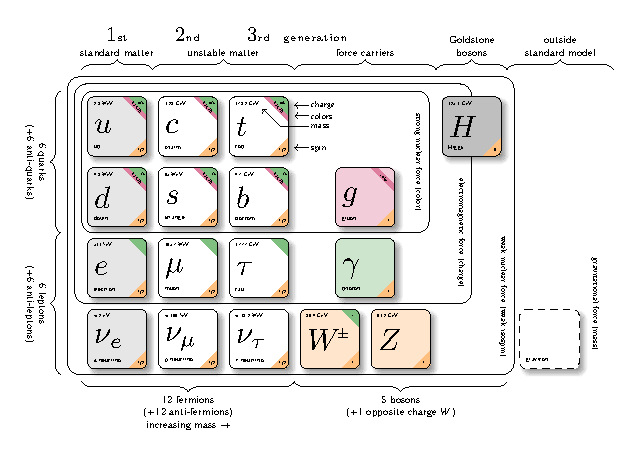
\includegraphics[width=1\textwidth]{Images/model-physics.pdf}
    \caption{Every elementary particle in the SM}
    \label{fig:SM}
\end{figure}

\subsubsection{Fermions} \label{sec:Fermions}
\input{Text/Chapters/Theory/Sections/StandardModel/Particles/Fermions}

\subsubsection{Bosons} \label{sec:Bosons}
\input{Text/Chapters/Theory/Sections/StandardModel/Particles/Bosons}

\subsection{Forces} \label{sec:Forces}

\subsubsection{The electromagnetic interaction} \label{sec:EMInteraction}
\input{Text/Chapters/Theory/Sections/StandardModel/Forces/EMInteraction}

\subsubsection{The weak interaction} \label{sec:WeakInteraction}
\input{Text/Chapters/Theory/Sections/StandardModel/Forces/WeakInteraction}

\subsubsection{The strong interaction} \label{sec:StrongInteraction}
\input{Text/Chapters/Theory/Sections/StandardModel/Forces/StrongInteraction}

\subsubsection{The Higgs field} \label{sec:Higgs}
\input{Text/Chapters/Theory/Sections/StandardModel/Particles/Higgs}

\section{Leptoquarks} \label{sec:Leptoquarks}
Many observed phenomena are conspicuously absent in the SM, confirming that while self-consistent, the SM is ultimately an incomplete theory. The gravitational force; the matter composition of the universe (including dark matter and dark energy); the matter-antimatter asymmetry in the universe; and massive, oscillating neutrinos, to name a few, all lack any prediction in the SM. Attempts to model these phenomena within the paradigm of QFT and merge them with the SM are often called extensions to the SM or beyond the SM theories. Some extensions to the SM, such as Grand Unification~\cite{gut1}\cite{gut2}, Technicolor~\cite{techni1}\cite{techni2}\cite{techni3}, composite models, and Supersymmetry~\cite{superstring}, require a new boson that would uniquely carry both baryon number $B$ and lepton number $L$, generically called a leptoquark (symbolically, \LQ). Such a boson would mediate quark-lepton transitions and answer many of the questions left in the SM, such as the remarkable symmetry of the quark and lepton generations.

\subsection{Models} \label{sec:LQModels}


Leptoquarks can be scalar (spin 0) or vector (spin 1) bosons, are color-triplets under \SUthreeC, carry fractional electric charge and weak isospin. Listed in Table~\ref{tab:LQModels} are the possible quantum numbers a leptoquark may take assuming dimensionless couplings to SM fermions and invariance under the gauge group of the SM. The first two columns list the spin and fermion quantum numbers, followed by the QCD and weak isospin representations, the weak hypercharge, and the allowed couplings to chiral SM fermions (color indices, flavor indices, and charge conjugates have been supressed). As the right-most column of Table~\ref{tab:LQModels} shows, leptoquarks may couple to only right-chiral fermions or left-chiral fermions, called chiral leptoquarks, or one left-chiral and one right-chiral fermion, called non-chiral leptoquarks. The allowed lepton and quark generations have historically been constrained to the same generation, motived by experimental limits placed on rare processes like proton decay, and FCNCs~\cite{FCNC}. However, as detailed in Section~\ref{sec:ExperimentalMotivation}, allowing intergenerational mixing can provide an explaination for phenomena like the flavor anomalies and muon magnetic moment anomaly. 

For a given leptoquark model there are also a set of free parameters, which include the mass \MLQ the Yukawa coupling at the leptoquark-quark-lepton vertex $\lambda$, and the decay branching fraction into a charged lepton $\beta$ (with $\beta-1$ the branching fraction into a neutrino). Specific to vector leptoquark models are two additional parameters $\lambda_{\text{G}}$ and $\kappa_{\text{G}}$ that correspond to the couplings of leptoquarks to SM gauge bosons at the \HepProcess{\Pgluon\LQ} and \HepProcess{\Pgluon\Pgluon\LQ} vertices. The LHC is capable of both single- and pair-production of leptoquarks through large QCD cross sections, as shown in Figs.~\ref{fig:LQsingleprod} and~\ref{fig:LQpairprod}. 

\begin{table}[H]
    \begin{center}
        \caption{List of quantum numbers and allowed couplings to quarks/leptons for different leptoquark models.}
        \begin{tabular}{cccccl}
            \hline \hline
            Spin    & $3B+L$    & \SUthreeC                                 & \SUtwoW   & \UoneY        & Allowed coupling \\ \hline
            \num{0} & \num{-2}  & \num[parse-numbers=false]{\overline{3}}   & \num{1}   & \num{1/3}     & $\antispinor{\Pquark}{L}{c}\spinor{\Plepton}{L}{}$ or $\antispinor{\Pup}{R}{c}\spinor{\Pe}{R}{}$ \\ 
            \num{0} & \num{-2}  & \num[parse-numbers=false]{\overline{3}}   & \num{1}   & \num{4/3}     & $\antispinor{\Pdown}{R}{c}\spinor{\Pe}{R}{}$ \\ 
            \num{0} & \num{-2}  & \num[parse-numbers=false]{\overline{3}}   & \num{3}   & \num{1/3}     & $\antispinor{\Pquark}{L}{c}\spinor{\Plepton}{L}{}$ \\ 
            \num{1} & \num{-2}  & \num[parse-numbers=false]{\overline{3}}   & \num{2}   & \num{5/6}     & $\antispinor{\Pquark}{L}{c}\gammamu\spinor{\Pe}{R}{}$ or $\antispinor{\Pdown}{R}{c}\gammamu\spinor{\Plepton}{L}{}$ \\ 
            \num{1} & \num{-2}  & \num[parse-numbers=false]{\overline{3}}   & \num{2}   & \num{-1/6}    & $\antispinor{\Pup}{R}{c}\gammamu\spinor{\Plepton}{L}{}$ \\ 
            \num{0} & \num{0}   & \num{3}                                   & \num{2}   & \num{7/6}     & $\antispinor{\Pquark}{L}{}\spinor{\Pe}{R}{}$ or $\antispinor{\Pup}{R}{}\spinor{\Plepton}{L}{}$ \\ 
            \num{0} & \num{0}   & \num{3}                                   & \num{2}   & \num{1/6}     & $\antispinor{\Pdown}{R}{}\spinor{\Plepton}{L}{}$ \\ 
            \num{1} & \num{0}   & \num{3}                                   & \num{1}   & \num{2/3}     & $\antispinor{\Pquark}{L}{}\gammamu\spinor{\Plepton}{L}{}$ or $\antispinor{\Pdown}{R}{}\gammamu\spinor{\Pe}{R}{}$ \\ 
            \num{1} & \num{0}   & \num{3}                                   & \num{1}   & \num{5/3}     & $\antispinor{\Pup}{R}{}\gammamu\spinor{\Pe}{R}{}$ \\ 
            \num{1} & \num{0}   & \num{3}                                   & \num{3}   & \num{2/3}     & $\antispinor{\Pquark}{L}{}\gammamu\spinor{\Plepton}{L}{}$ \\ \hline \hline
        \end{tabular}
        \label{tab:LQModels}
    \end{center}
\end{table}

\begin{figure}[H]
    \centering
    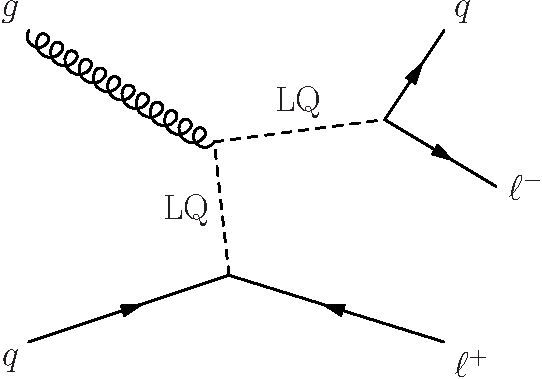
\includegraphics[width=0.3\textwidth]{Images/Theory/SingleLQProdT1.pdf}\hspace{0.1\textwidth}
    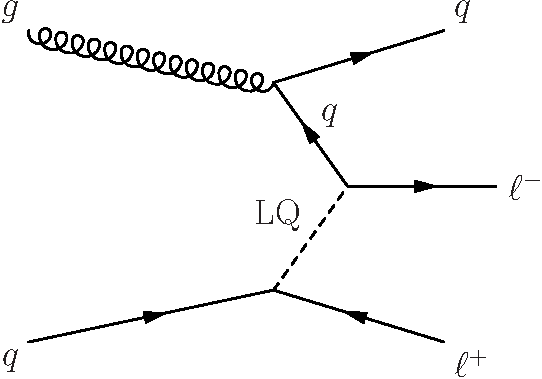
\includegraphics[width=0.3\textwidth]{Images/Theory/SingleLQProdT2.pdf}\vspace{0.05\textwidth}
    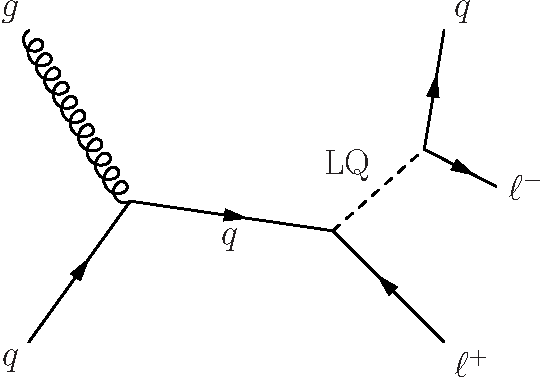
\includegraphics[width=0.3\textwidth]{Images/Theory/SingleLQProdS1.pdf}\vspace{0.05\textwidth}
    \caption{Production mechanisms of single leptoquarks at the LHC. Clockwise from top left: a t-channel processes that results in a resonant \HepProcess{\Pquark\Plepton} pair and a non-resonant \Plepton, a t-channel processes resulting in a non-resonant \HepProcess{\Plepton\Plepton\Pquark} final state, and an t-channel process resulting in a resonant \HepProcess{\Pquark\Plepton} pair and a non-resonant \Plepton.}
    \label{fig:LQsingleprod}
\end{figure}

\begin{figure}[H]
    \centering
    \includegraphics[width=0.3\textwidth]{Images/Theory/LQLQProduction_1.pdf}\hspace{0.1\textwidth}
    \includegraphics[width=0.3\textwidth]{Images/Theory/LQLQProduction_3.pdf}\vspace{0.05\textwidth}
    \includegraphics[width=0.3\textwidth]{Images/Theory/LQLQProduction_2.pdf}\hspace{0.1\textwidth}
    \includegraphics[width=0.3\textwidth]{Images/Theory/LQLQProduction_4.pdf}\vspace{0.05\textwidth}
    \caption{Production mechanisms of \HepProcess{\LQ\LQbar} pairs at the LHC. Clockwise from top-left: s-channel gluon-gluon fusion, gluon-gluon four-point interaction, t-channel gluon-gluon interaction via leptoquark exchange, and s-channel quark-antiquark annihilation.}
    \label{fig:LQpairprod}
\end{figure}

\subsection{Experimental motivation} \label{sec:ExperimentalMotivation}
% Flavor anomalies (LHCb)

The SM assumes that the weak gauge bosons couple to each lepton flavor identically (or close to it), a phenomenon called lepton flavor universality. Tests of lepton flavor universality can be performed by studying flavor-changing neutral current (FCNC) transitions, such as when a bottom quark transforms into strange quark in the decay: $B^+\rightarrow K^+\ell^+\ell^-$. As FCNC are suppressed at tree-level in the SM, occuring only via higher order electroweak processes (as shown in the left-hand diagram of Fig.~\ref{fig:FCNC}), these decays are a powerful probe into new physics. Measurements by the LHCb, BaBar, and Belle collaborations of observables such as $R_K$, $R_{K*}$, $R_D$, and $R_{D*}$---the decay branching fractions of $B$ mesons into an electron-positron pair over a muon-antimuon pair---hint at a possible violation of lepton flavor universality. Combining the flavor anomalies from each collaboration in $R_K^*$ (Fig.~\ref{fig:FlavorAnomalies}, left) yields tension between experiment and the SM at 2 standard deviations~\cite{LHCb1}, and for $R_K$ (Fig.~\ref{fig:FlavorAnomalies}, right) up to 3.1 standard deviations~\cite{LHCb2}. Leptoquarks coupling to muons and bottom quarks are prime candidates to explain these flavor anomalies at tree-level, as shown in the right-hand diagram of Fig.~\ref{fig:FCNC}.

\begin{figure}[H]
    \centering
    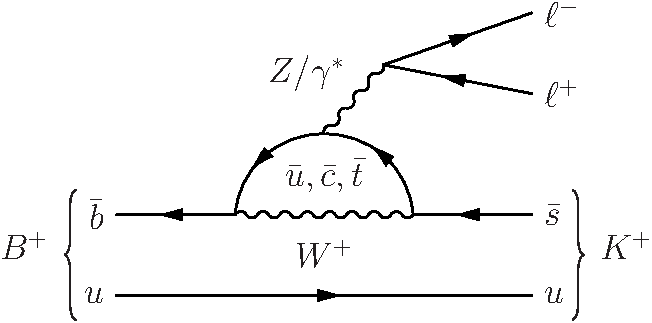
\includegraphics[width=0.4\textwidth]{Images/BplusDecayFCNC.pdf}\hspace{0.1\textwidth}
    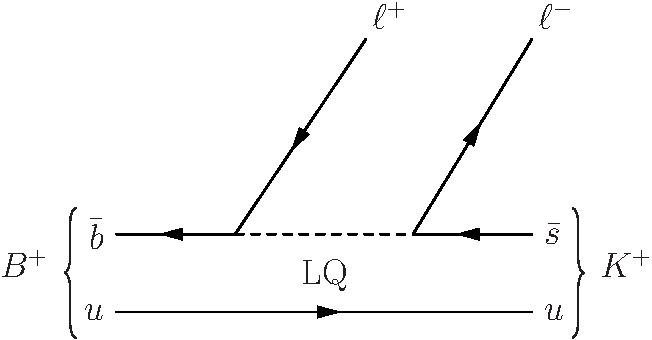
\includegraphics[width=0.4\textwidth]{Images/BplusDecayLQ.pdf}
    \caption{The decay of a charged $B$ meson into a charged kaon and a pair of opposite-sign charged leptons. Left: An example of a loop diagram FCNC process in the SM that is strongly suppressed. Right: A tree-level FCNC solution with a leptoquark mediating the transition.}
    \label{fig:FCNC}
\end{figure}

\begin{figure}[H]
    \centering
    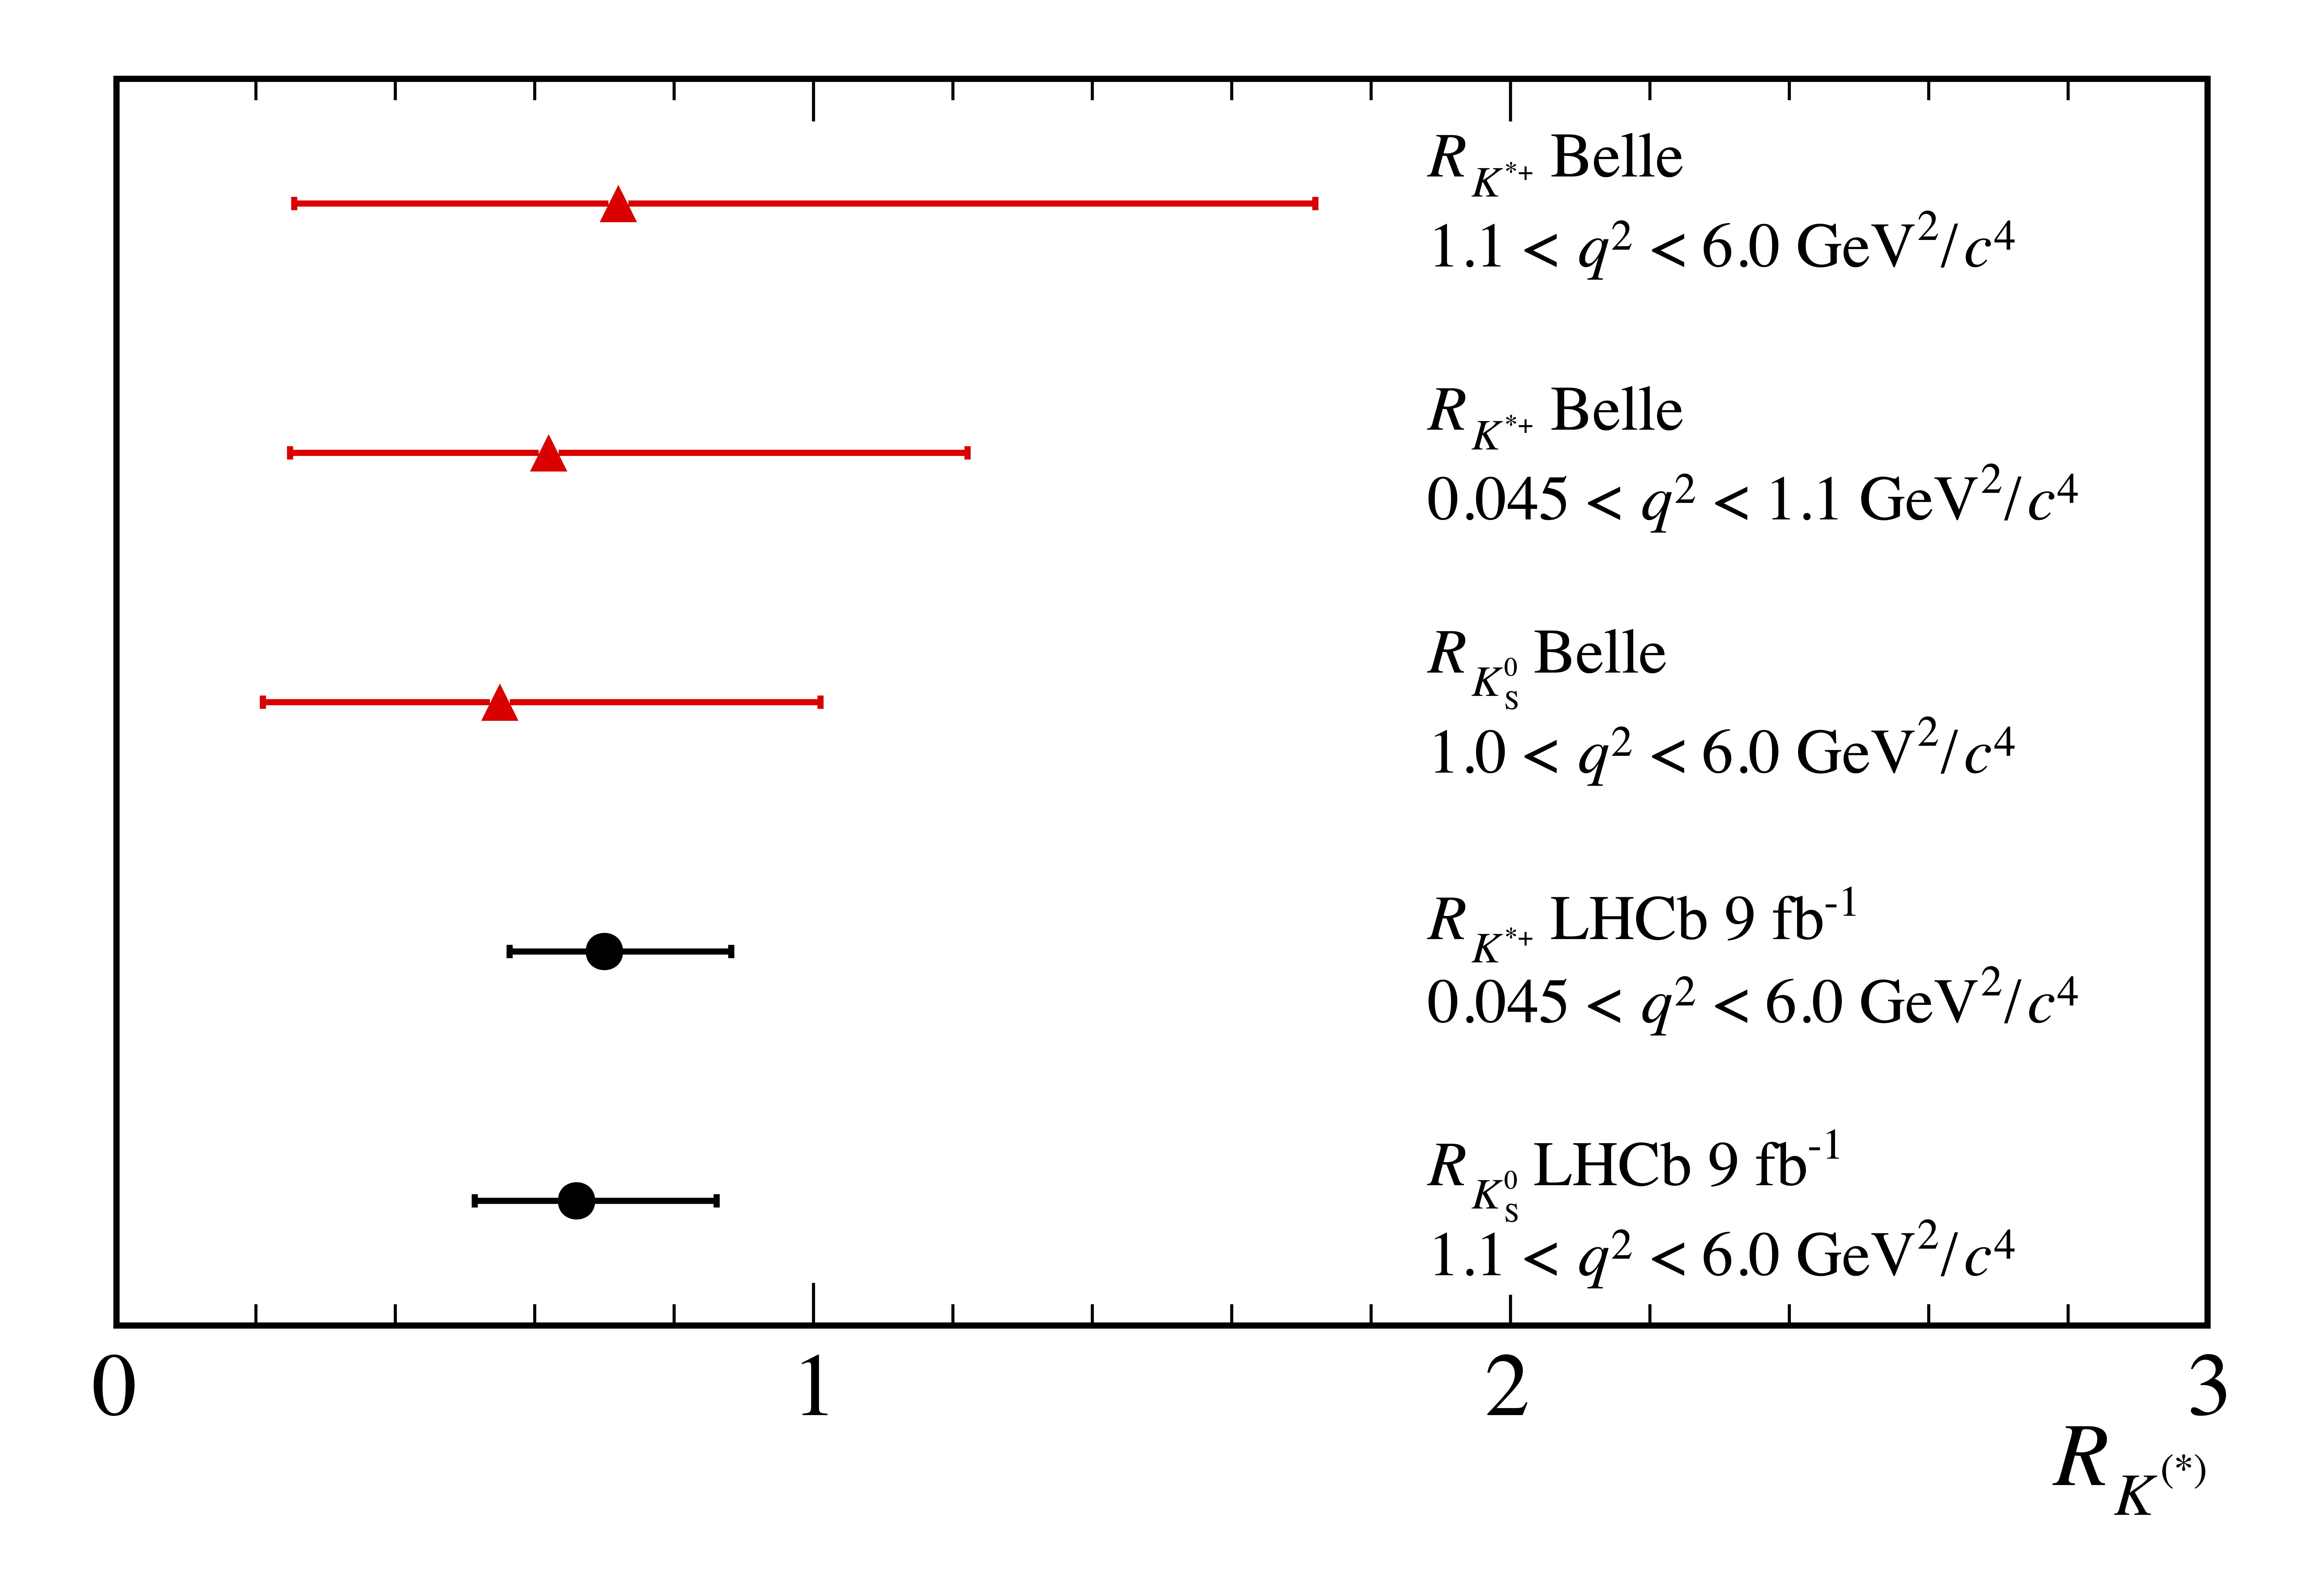
\includegraphics[width=0.49\textwidth]{Images/LHCbBelle.png}
    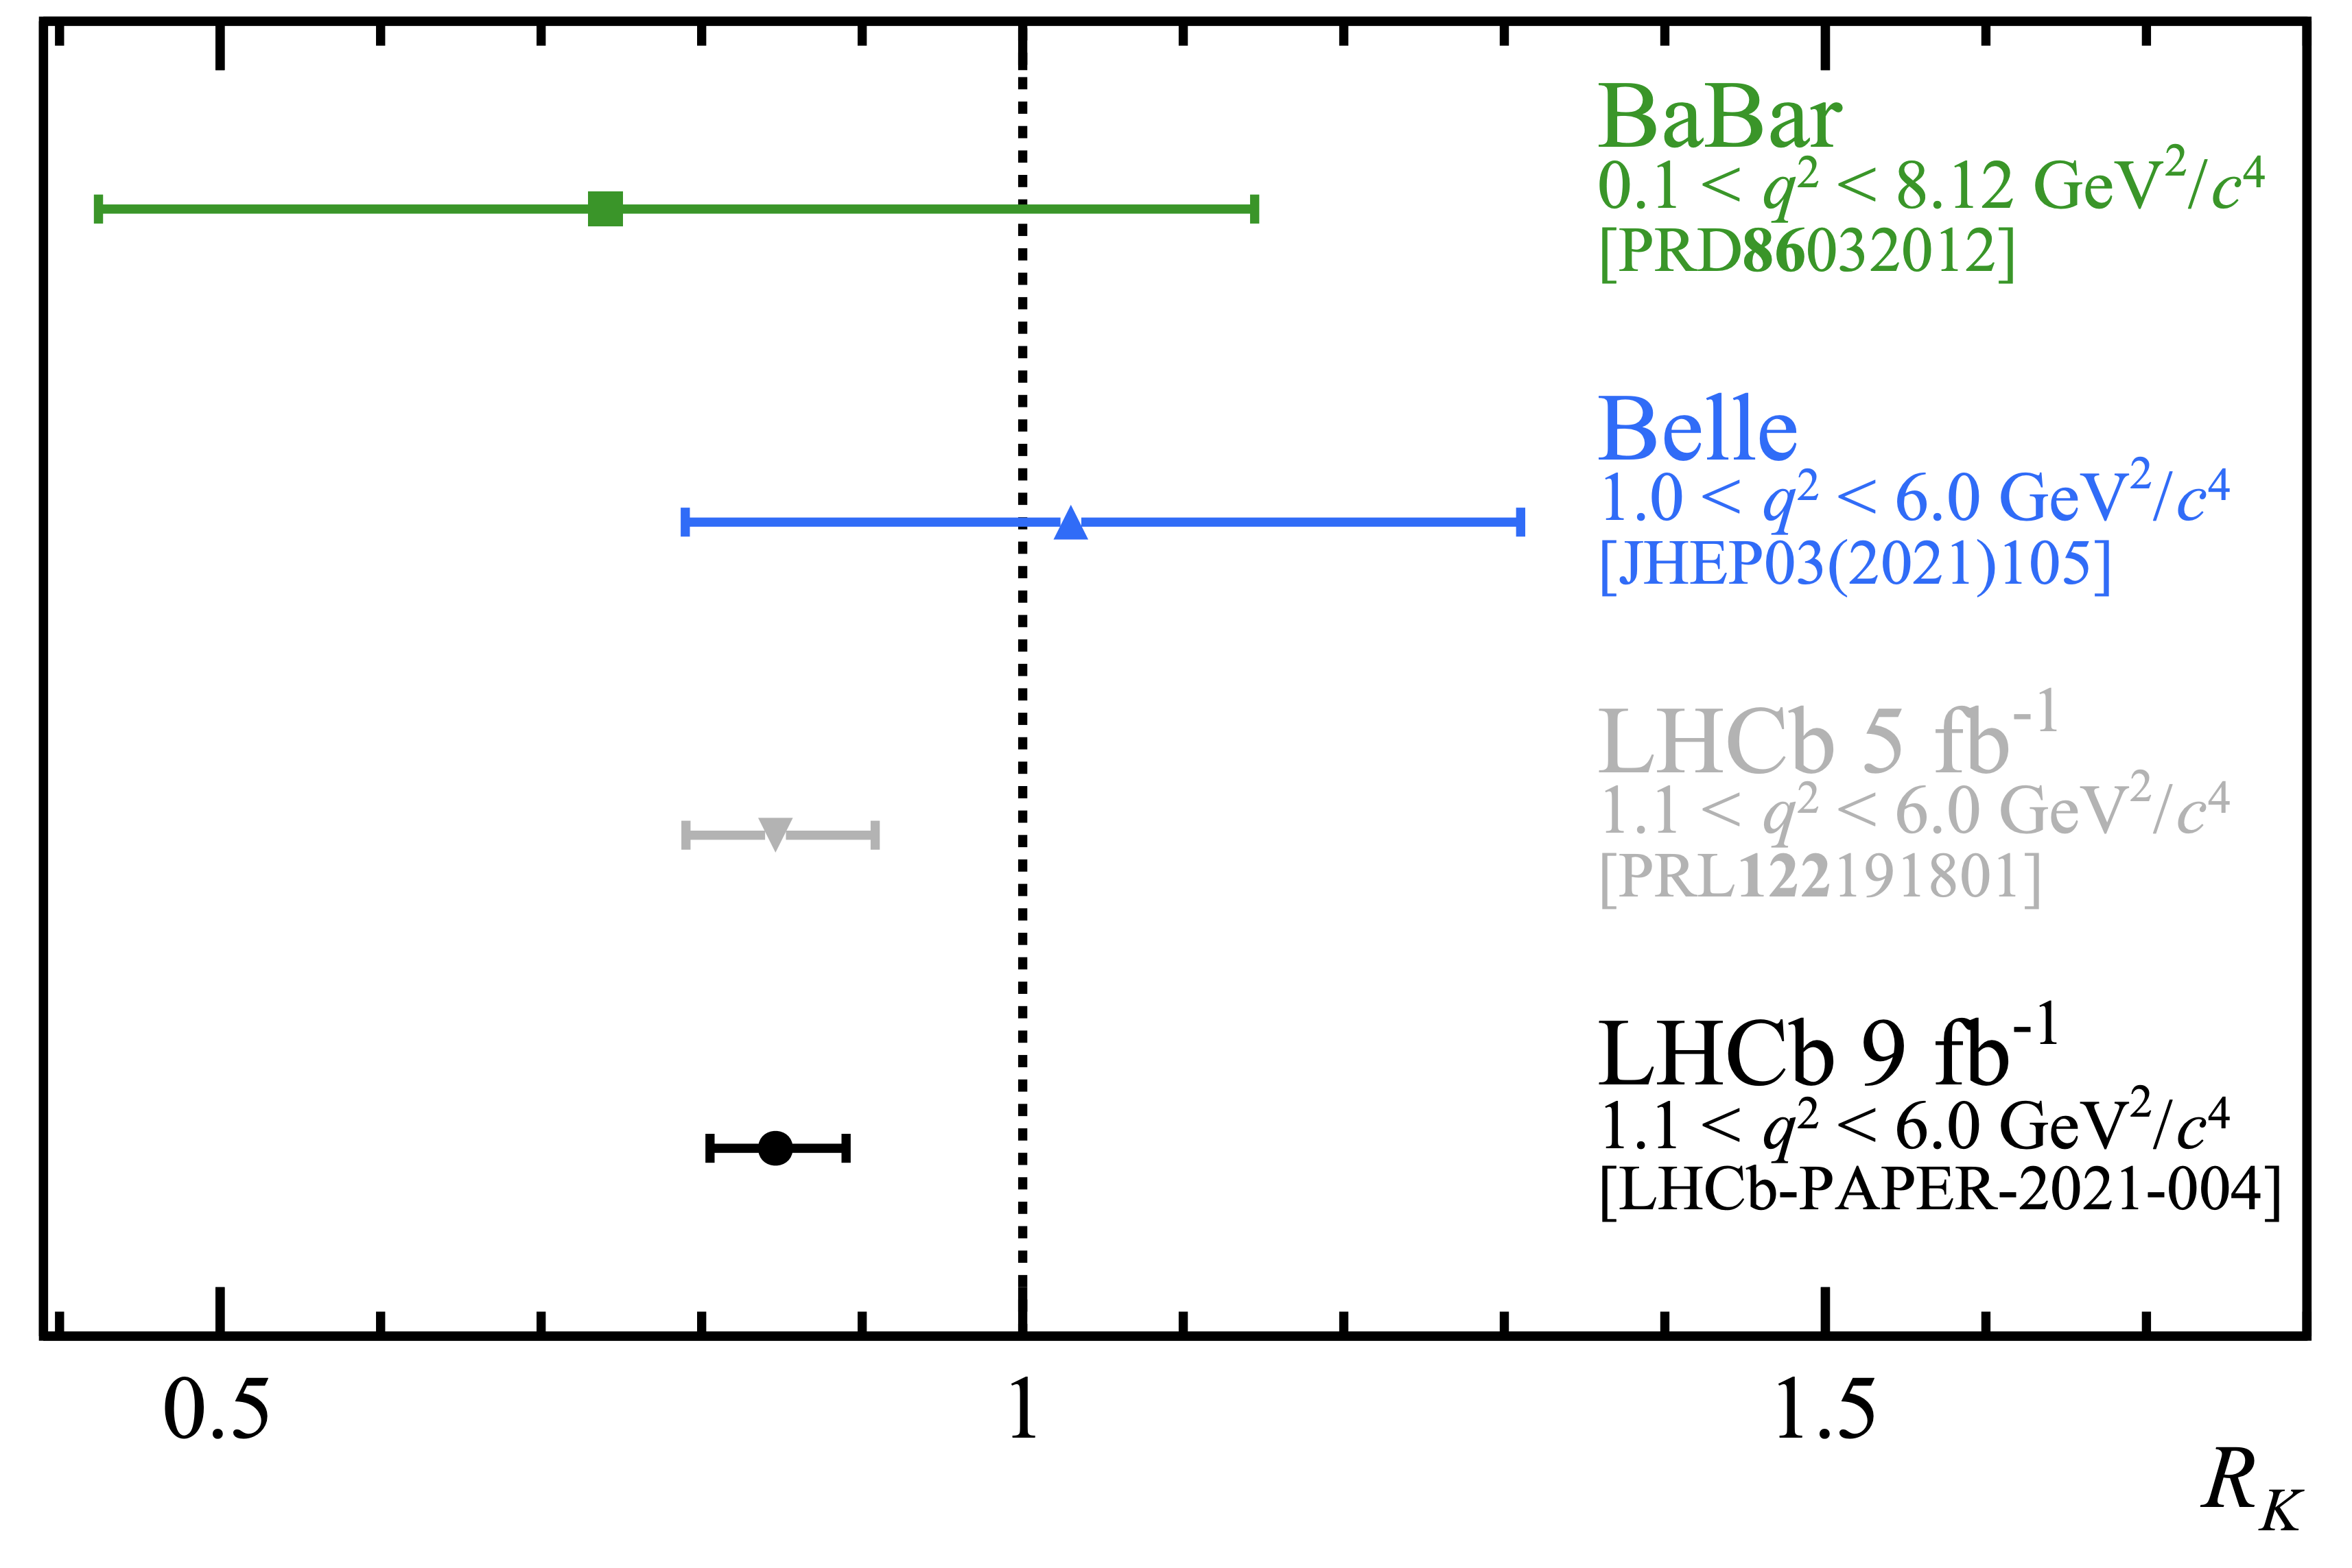
\includegraphics[width=0.49\textwidth]{Images/RKmeasurements.png}
    \caption{Left: A comparison of $R_{K*}$ measurements by the Belle and LHCb collaborations for several bands of the dilepton invariant mass squared $q^2$. Right: A comparison of $R_K$ measurements (combining $B^+\rightarrow K^+\ell^+\ell^-$ and $B^0\rightarrow K^0_s\ell^+\ell^-$ decays) by the BaBar, Belle, and LHCb collaborations for several bands of the dilepton invariant mass squared $q^2$.}
    \label{fig:FlavorAnomalies}
\end{figure}

% Muon magnetic moment anomaly (Muon g-2)

Another notable inconsistency between the SM prediction and experiment in which leptoquarks may play a role is the anomalous muon magentic dipole moment. The magnetic moment of the muon is defined as:

\begin{equation}
    \vec{\mu} = g_{\mu}\left(\frac{q}{2m_{\mu}}\right)\vec{s}
\end{equation}
where the factor $g_{\mu}$ as predicted by the Dirac equation is equal to 2. Considering a number of EM, EW, and QCD radiative corrections (a few example diagrams are shown in Fig.~\ref{fig:amu}, left), the SM value of $g_{\mu}$ is predicted with high precision to deviate from 2, encapsulated in the muon magnetic anomaly $a_{\mu} = (g_{\mu}-2)/2$. Recent calculations set the SM theoretical value $a_{\mu}(\mathrm{SM})=\num{116591810(43)e-11}$, a precision of 0.37 parts-per-million (ppm). Measurements of $a_{\mu}$ by the Muon $g-2$ experiment at Brookhaven National Laboratory (BNL) and Fermilab National Accelerator Laboratory (FNAL) found a combined experimental average of $a_{\mu}(\mathrm{Exp}) = \num{116592061(41)e-11}$, with an astonishing precision of 0.34 ppm~\cite{Muongminus2}, as shown in Fig.~\ref{fig:amuExp}. The difference between the theoretical prediction and the experimental average has a significance of 4.2 standard deviations. Introducing leptoquarks that couple to muons could explain the deviation form the SM, as seen in the diagram in Fig.~\ref{fig:amuLQ}.

\begin{figure}[H]
    \centering
    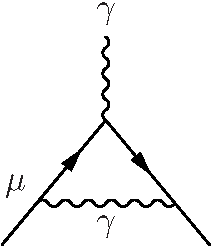
\includegraphics[width=0.2\textwidth]{Images/Muon_gminus2_photon.pdf}\hspace{0.05\textwidth}
    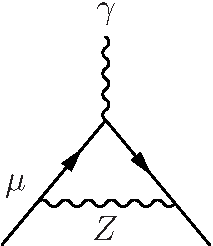
\includegraphics[width=0.2\textwidth]{Images/Muon_gminus2_Z.pdf}\hspace{0.05\textwidth}
    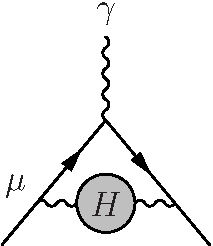
\includegraphics[width=0.2\textwidth]{Images/Muon_gminus2_Hadronic.pdf}\hspace{0.05\textwidth}
    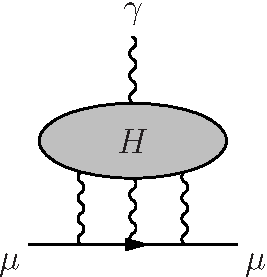
\includegraphics[width=0.2\textwidth]{Images/Muon_gminus2_Hadronic2.pdf}
    \caption{The Feynman diagrams of SM contributions to the muon anomaly. From left to right: the first-order QED and weak processes, leading-order hadronic vacuum polarization, and hadronic light-by-light contributions.}
    \label{fig:amu}
\end{figure}

\begin{figure}[H]
    \centering
    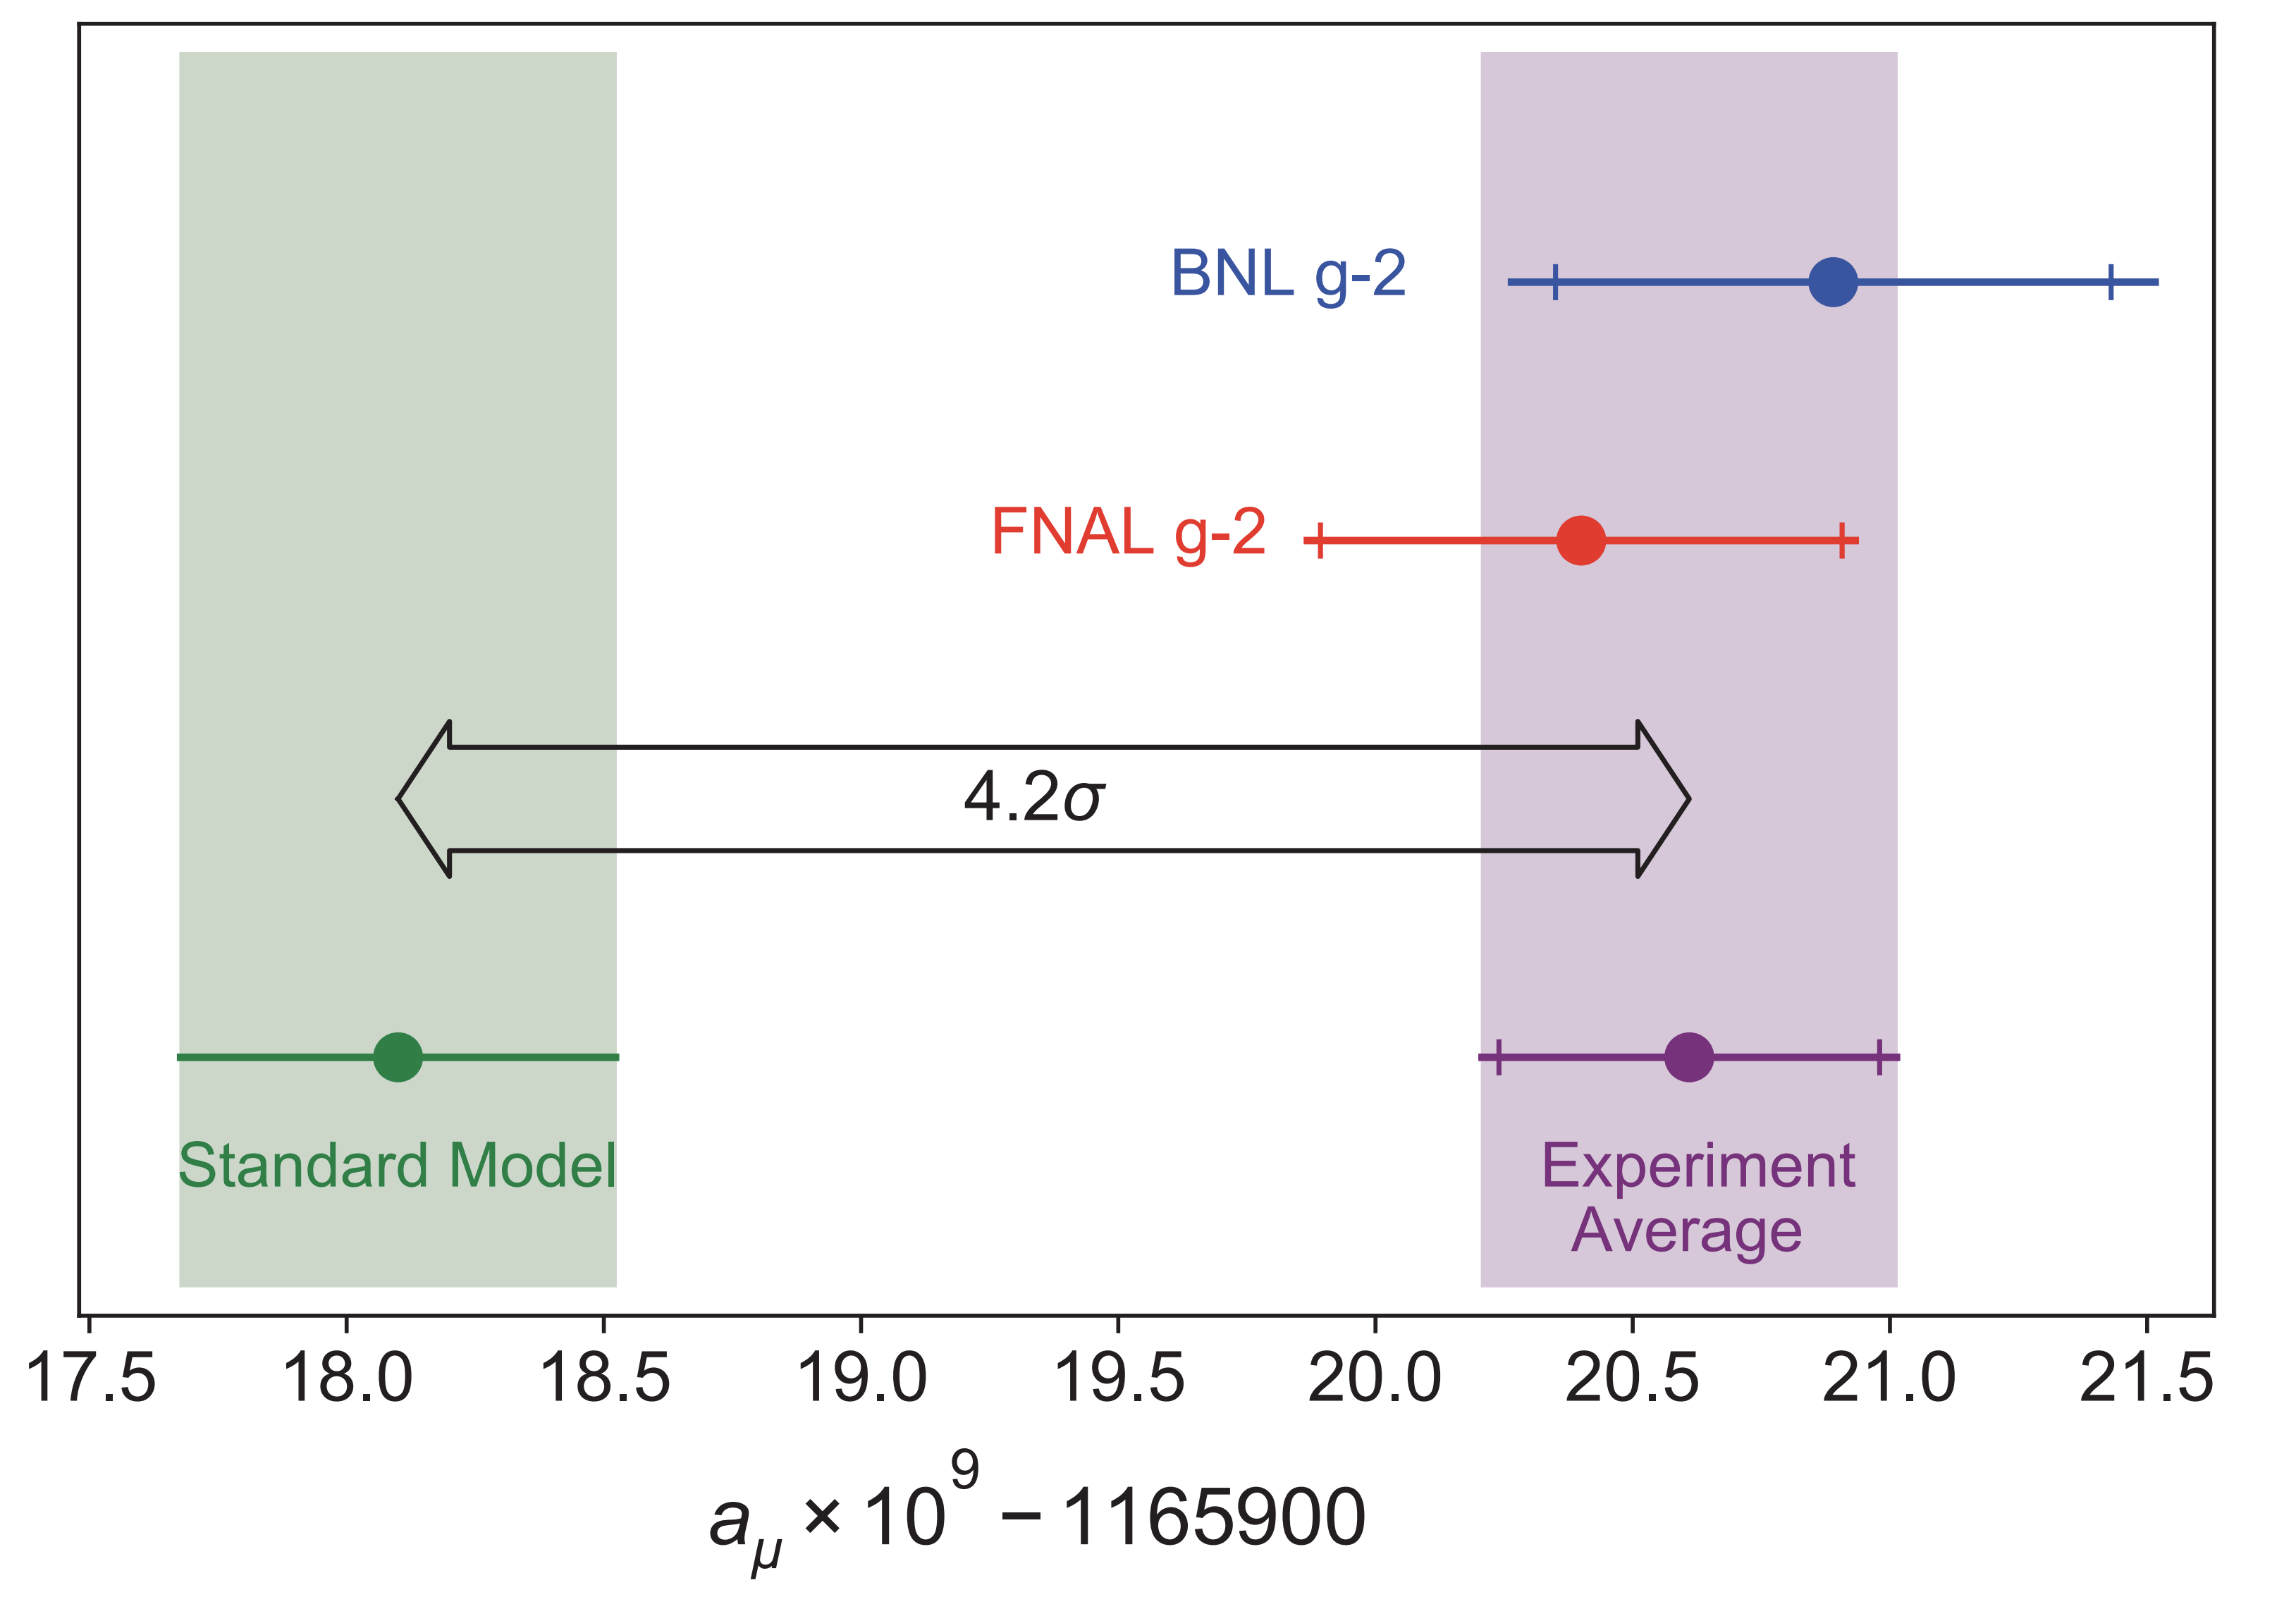
\includegraphics[width=0.7\textwidth]{Images/MuonAnomaly.png}
    \caption{A comparison of $a_\mu$ measured by BNL, FNAL, and the combined average beside the SM prediction.}
    \label{fig:amuExp}
\end{figure}

\begin{figure}[H]
    \centering
    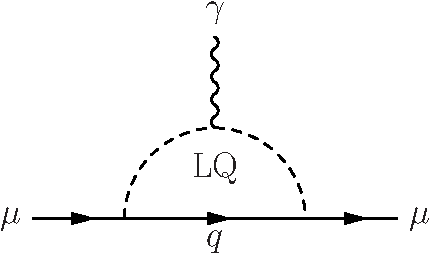
\includegraphics[width=0.5\textwidth]{Images/Muon_gminus2_LQ.pdf}
    \caption{A Feynman diagram of a leptoquark solution to the magnetic anomaly $a_{\mu}$.}
    \label{fig:amuLQ}
\end{figure}

\subsection{This search} \label{sec:ThisSearch}
The leptoquark search detailed in Chapter~\ref{chapter:LeptoquarkSearch} considers only pair-produced scalar leptoquarks that couple to a bottom quark and muon, but is otherwise model independent. These search parameters constrain $\lambda_G$ and $\kappa_G$ to zero, $\beta$ to unity, and keeps the search insensitive to $\lambda$, leaving $M_{\LQ}$ the only search variable. Previous limits on leptoquark masses~\cite{} motivate a mass scan of 30 points ranging from 300~GeV to 4000~GeV. This search is the first leptoquark search with muons in the final state to analyze the entire LHC Run II dataset collected by CMS and the first ever search for the process $\LQ\LQ\rightarrow\mu\mu bb$ by CMS.


\chapter{Experimental Setup: The LHC and the CMS Detector} \label{chapter:Experiment}
\section{The Large Hadron Collider} \label{sec:LHC}
The Large Hadron Collider (LHC) \cite{LHCTDR} is a dual-ring high-energy particle accelerator and collider located at CERN, the European Laboratory for Particle Physics, in Geneva, Switzerland. Built in the tunnel of the dismantled LEP collider $\SI{50}{m}$ below the Swiss-French border (see Fig.~\ref{fig:LHC}), the LHC spans $\SI{27}{km}$ in circumference and currently holds the world record for the highest-energy particle collisions at a center-of-mass energy $\sqrt{s} = \SI{13}{TeV}$. Four independent detectors located at points along the circumference of the LHC record the collisions: Compact Muon Solenoid (CMS), A Toroidal LHC ApparatuS (ATLAS), Large Hadron Collider beauty (LHCb), and A Lead Ion Collider Experiment (ALICE).

\begin{figure}[H]
    \centering
    \resizebox{1\textwidth}{!}{
    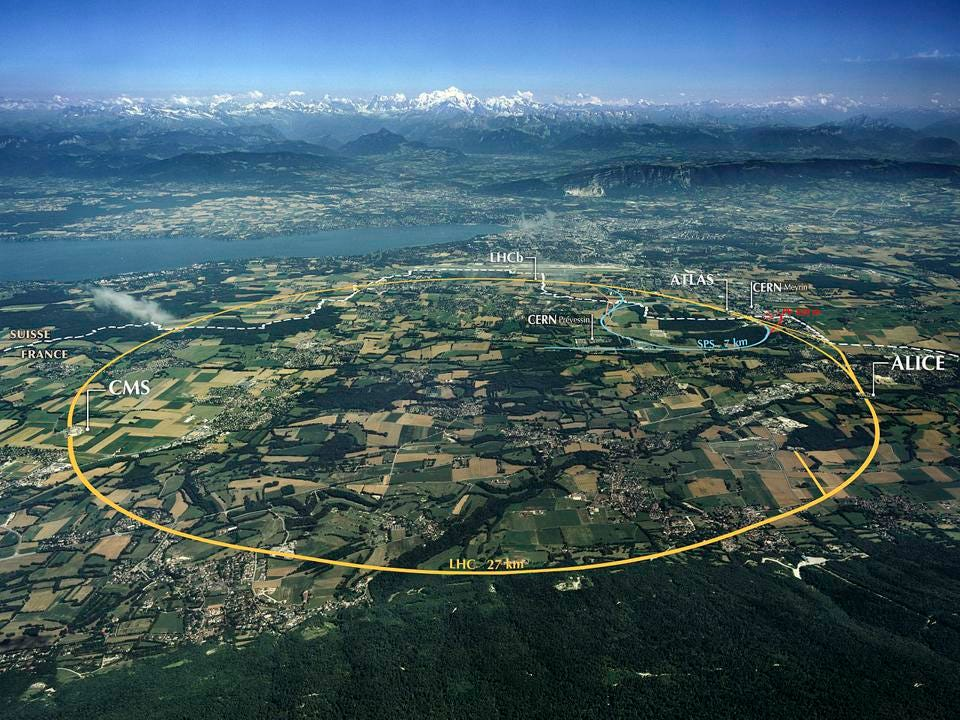
\includegraphics[height=\textwidth]{Images/CMS/LHCring.jpg}
    \quad
    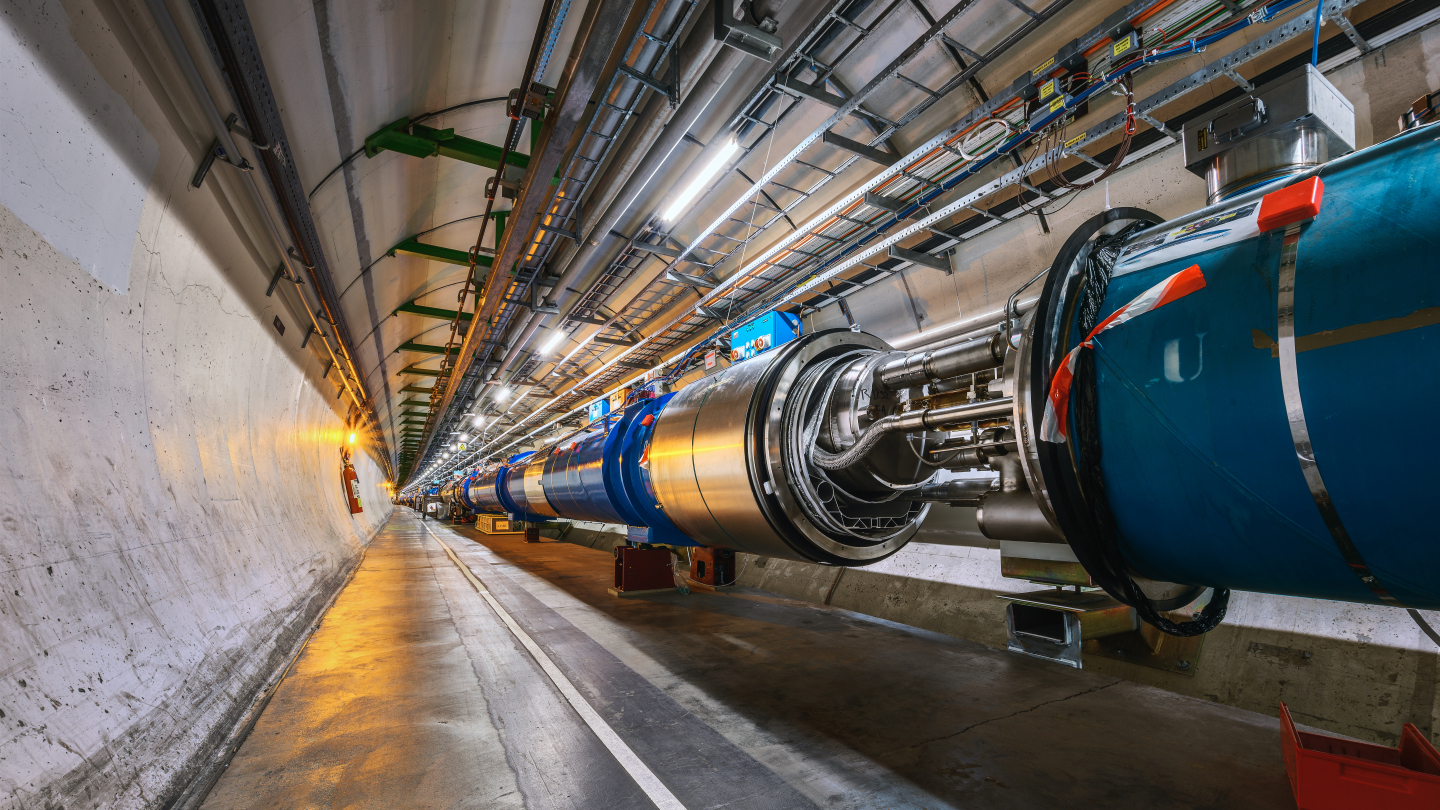
\includegraphics[height=\textwidth]{Images/CMS/LHCpipe.jpg}
    }
    \caption{Left: A tracing of the LHC tunnel over the Swiss-French border near Geneva. Right: A section of the LHC beam pipe in the underground LHC tunnel.}
    \label{fig:LHC}
\end{figure}

Within the LHC, two beams of protons or heavy ions are accelerated in opposite directions, captured and stored by $\SI{400}{MHz}$ radiofrequency (RF) cavities located at 16 points along the LHC ring that longitudinally sort the beams into 2808 bunches of $\SI{1.15e11}{}$ protons or Pb ions, with each bunch spaced $\SI{25}{ns}$ apart. The beams at the LHC are steered along each ring by 1232 $\SI{8.3}{T}$ superconducting dipole magnets, while 392 superconducting quadrupole magnets focus the beams into a narrow transverse cross section of $\SI{3.8}{\micro\meter}$. The beams cross at four insertion points along the LHC, where the proton-proton or lead ion collisions occur and are recorded by each of the four LHC experiments.

The LHC was designed to operate in several sequential phases. Phase-1 saw first collisions at $\sqrt{s}=\SI{7}{TeV}$ in 2010 which was increased to $\sqrt{s}=\SI{13}{TeV}$ in 2015. Phase-2 of the LHC will raise the instantanious luminosity by a factor of ten, called the High-Luminosity LHC (HL-LHC) era, slated to begin operation in 2027. Upgrades to the LHC and detectors are performed during long shutdown (LS) periods that separate data-taking runs.

The physics goals of the LHC could be broadly summerized with the following: to observe the last undiscovered particle in the SM, the Higgs boson; to search for evidence of beyond the SM physics; and to perform precision measurements of existing SM phenomena. On July 4th, 2012 it was announced that the ATLAS and CMS collaborations had independently observed the Higgs boson, which remains the hallmark achievement at the LHC.

\section{The CMS detector} \label{sec:CMS}
\subsection{Tracker} \label{sec:InnerTracker}

The inner-most detector, closest to the beam pipe, is the CMS tracker system, which uses two technologies: silicon pixels and silicon microstrips (photos of each shown in Fig.~\ref{fig:Tracker}). The purpose of the CMS tracking system is to reconstruct the trajectories of electromagnetically charged physics objects close to the interaction point and measure the positions of the primary vertex (PV) of collisions and secondary vertecies of displaced decays (e.g., B hadrons). Owing to its proximity to the primary-interaction point, the CMS tracker is subject to the highest dosage radiation of all the subsystems.

\begin{figure}[H]
    \centering
    \resizebox{1\textwidth}{!}{
    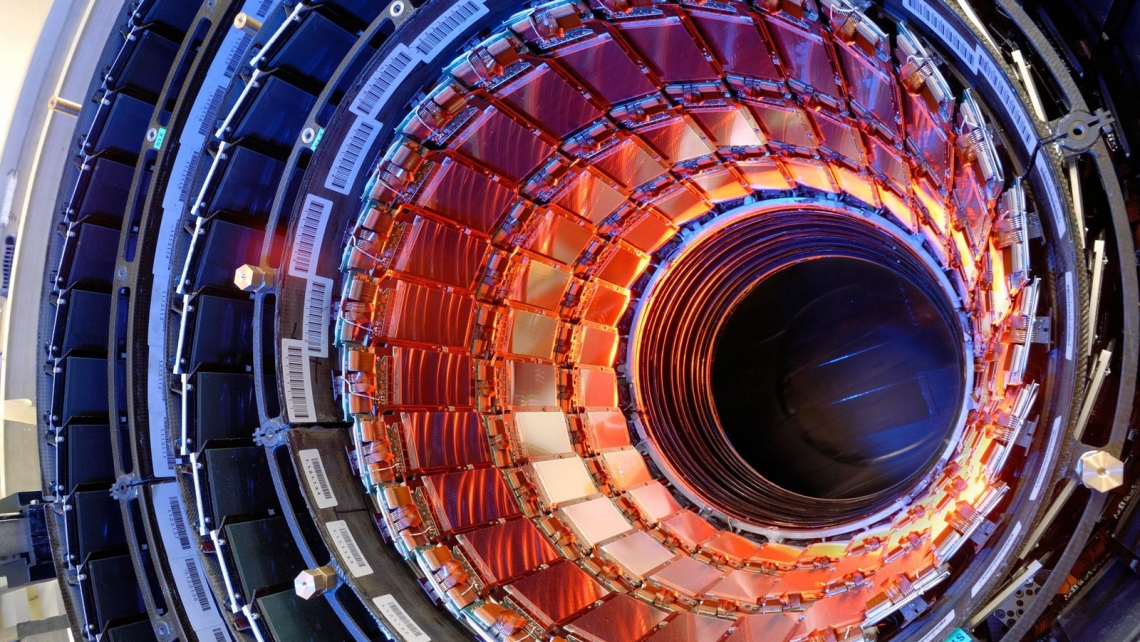
\includegraphics[height=\textwidth]{Images/CMS/SiStripTracker.jpg}
    \quad
    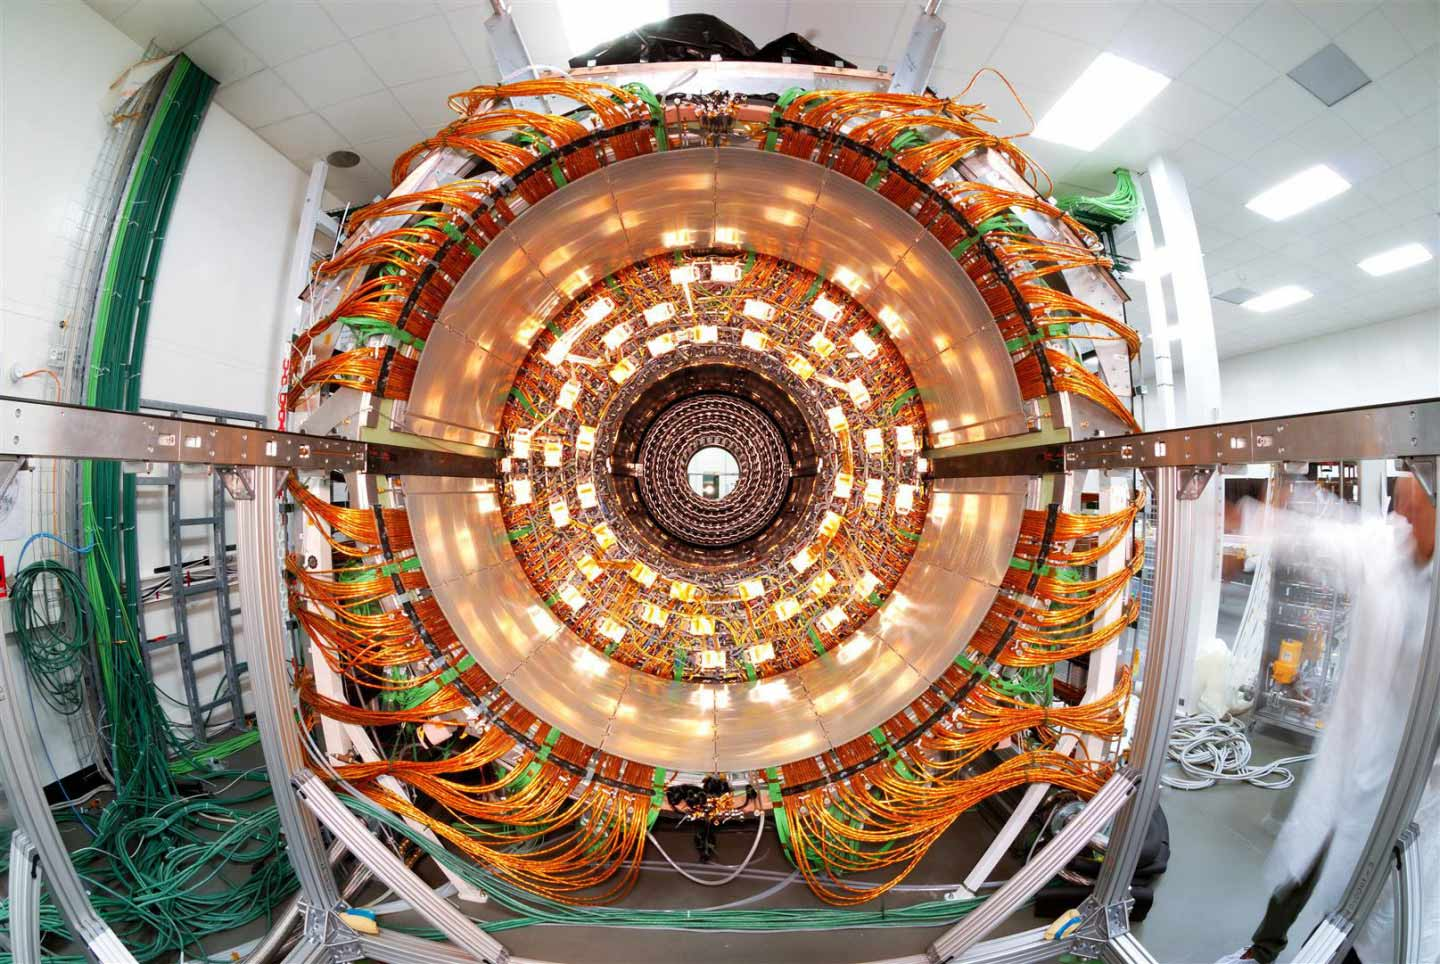
\includegraphics[height=\textwidth]{Images/CMS/PixelTracker.jpg}
    } 
    \caption{Photographs of the silicon strip detectors (left) and the pixel detectors (right) in the tracker barrel prior to installation.}
    \label{fig:Tracker}
\end{figure}

\subsubsection{Pixel tracker} \label{sec:PixelTracker}

The silicon pixel detector, upgraded to the Phase-1 pixel detector \cite{PixelUpgrade} during the 2016-2017 year-end technical stop of Run 2 to cope with higher integrated luminosities, provides a four-hit coverage in the pseudorapidity range $|\eta|<2.5$. This is accomplished through silicon sensor modules, where each module is a $160\times 416$ pixel sensor connected to 16 readout chips. The modules are arranged in two configurations: four concentric barrel pixel detectors (BPIX) with 1,184 modules, and three endcap disk pixel detectors in the forward regions (FPIX) with 672 modules, for a total of 1856 silicon sensor modules and 124 million readout channels. A schematic of the upgraded Phase-1 pixel detector is provided in Fig.~\ref{fig:PixelDiagram} showing the pseudorapidity coverage.

\begin{figure}[H]
    \centering
    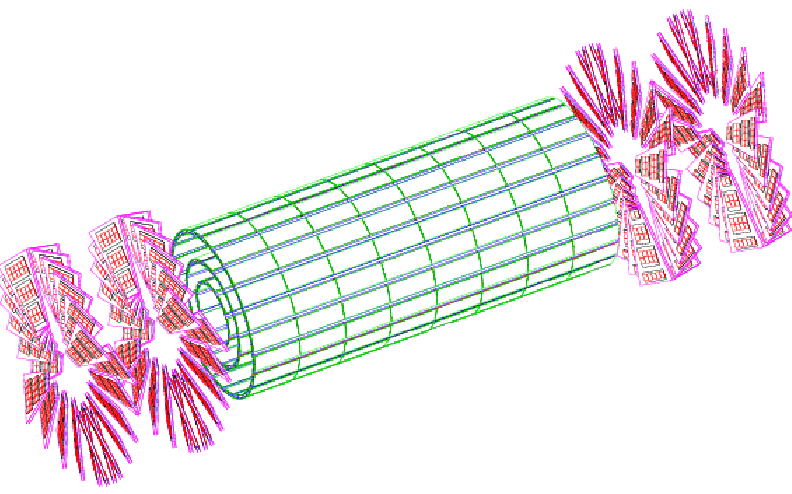
\includegraphics[width=\textwidth]{Images/CMS/PixelDiagram2.png}
    \caption{A diagram of the Phase-1 pixel detector with the BPIX drawn in green and the FPIX drawn in magenta.}
    \label{fig:PixelDiagram}
\end{figure}

\subsubsection{Strip tracker} \label{sec:StripTracker}

Surrounding the pixel detector is the silicon strip tracker \cite{SiliconStrip} which serves the same function as the pixel tracker and covers hits in the same pseudorapidity $|\eta|<2.5$ range. The silicon strip detector is also built with a modular structure, with 15,148 tracker modules each housing one or two silicon sensors totaling 24,244 strip sensors. The silicon strip tracker is divided into four sections: inner barrel (TIB), outer barrel (TOB), inner disks (TID), and outer endcaps (TEC). The TIB and TOB consist of four and six concentric shells respectively, while the TID consists of three disks in each of the forward regions, divided into three concentric rings, and the TEC consists of nine disks with four to seven concentric rings, also in the forward regions. A schematic of the silicon strip detector is provided in Fig.~\ref{fig:StripDiagram} showing the pseudorapidity coverage.

\begin{figure}[H]
    \centering
    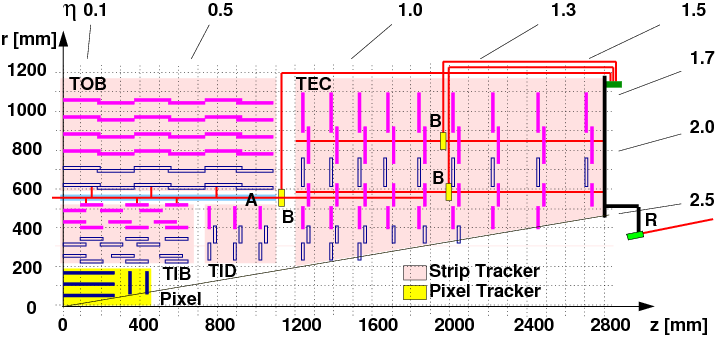
\includegraphics[width=\textwidth]{Images/CMS/TrackerQuadrant.png}
    \caption{A schematic cutaway showing one quadrant of the strip and pixel trackers.}
    \label{fig:StripDiagram}
\end{figure}

\subsection{Calorimeters} \label{sec:Calorimeters}
To measure the energy deposits of electromagnetic particles (e.g., electrons, photons) and hadrons (e.g., neutrons, mesons, jets), CMS relies on two calorimeters: the electromagnetic calorimeter and the hadronic calorimeter, both surrounding the CMS tracker and inside the solenoid magnet.

\subsubsection{The Electromagnetic Calorimeter} \label{sec:ECAL}
% Introduce detector, location, basic info (e.g., chamber count)
Immediately surrounding the CMS tracker is the CMS Electromagnetic Calorimeter (ECAL) \cite{ECALTDR}, which allows CMS to measure the energy deposits left by electrons and photons: highly-favored decay modes of the Higgs boson and critical in its discovery. To optimize performance, the ECAL was designed with the following performance goals: excellent energy and spacial resolution, hermeticity and high-granularity, fast particle identification and fast energy and isolation measurements at trigger-level, a wide energy range (\SI{5}{GeV} to \SI{5}{TeV}), and high radiation tolerance. Energy showers from electrons and photons are measured by an array of lead tungstate (PbWO$_4$) scintillating crystals (Fig.~\ref{fig:ECAL}, left). The ECAL is fully hermetic, composed of a barrel (EB) with a pseudorapidity coverage of $|\eta|<1.48$ and two endcaps (EE) that extend the range to $|\eta|<3.0$, (Cutaways of the EE and EB are shown on the right of Fig.~\ref{fig:ECAL}). Within the EB, crystals are grouped into 36 supermodules each containing 1700 crystals, and in each EE crystals are grouped into two dees with 3662 crystals in each, for a total of 75848 crystals in the ECAL. Crystals are oriented in a projective geometry, with an approximately $3^{\circ}$ tilt to avoid aligning crystal gaps with radial particle trajectories. Lining the inner faces of the EE dees in the range $1.65<|\eta|<2.6$ are preshower detectors (ES) made from lead absorbers and silicon strip sensors. A diagram of the ECAL showing the supermodule placement and pseudorapidity coverage is provided on the right of Fig.~\ref{fig:ECALDiagram}.

\begin{figure}[H]
    \centering
    \resizebox{1\textwidth}{!}{
    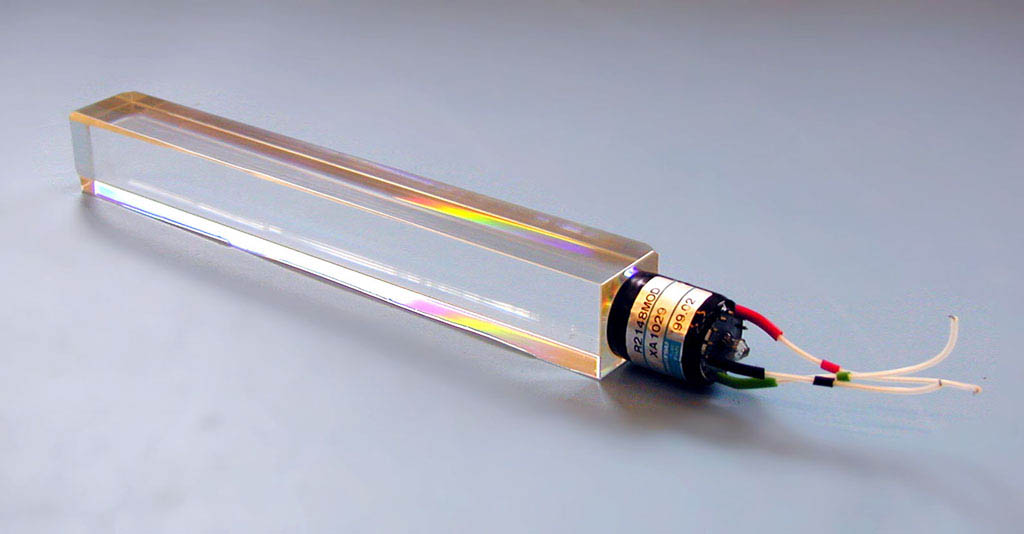
\includegraphics[height=\textwidth]{Images/CMS/ECALCrystal.jpg}
    \quad
    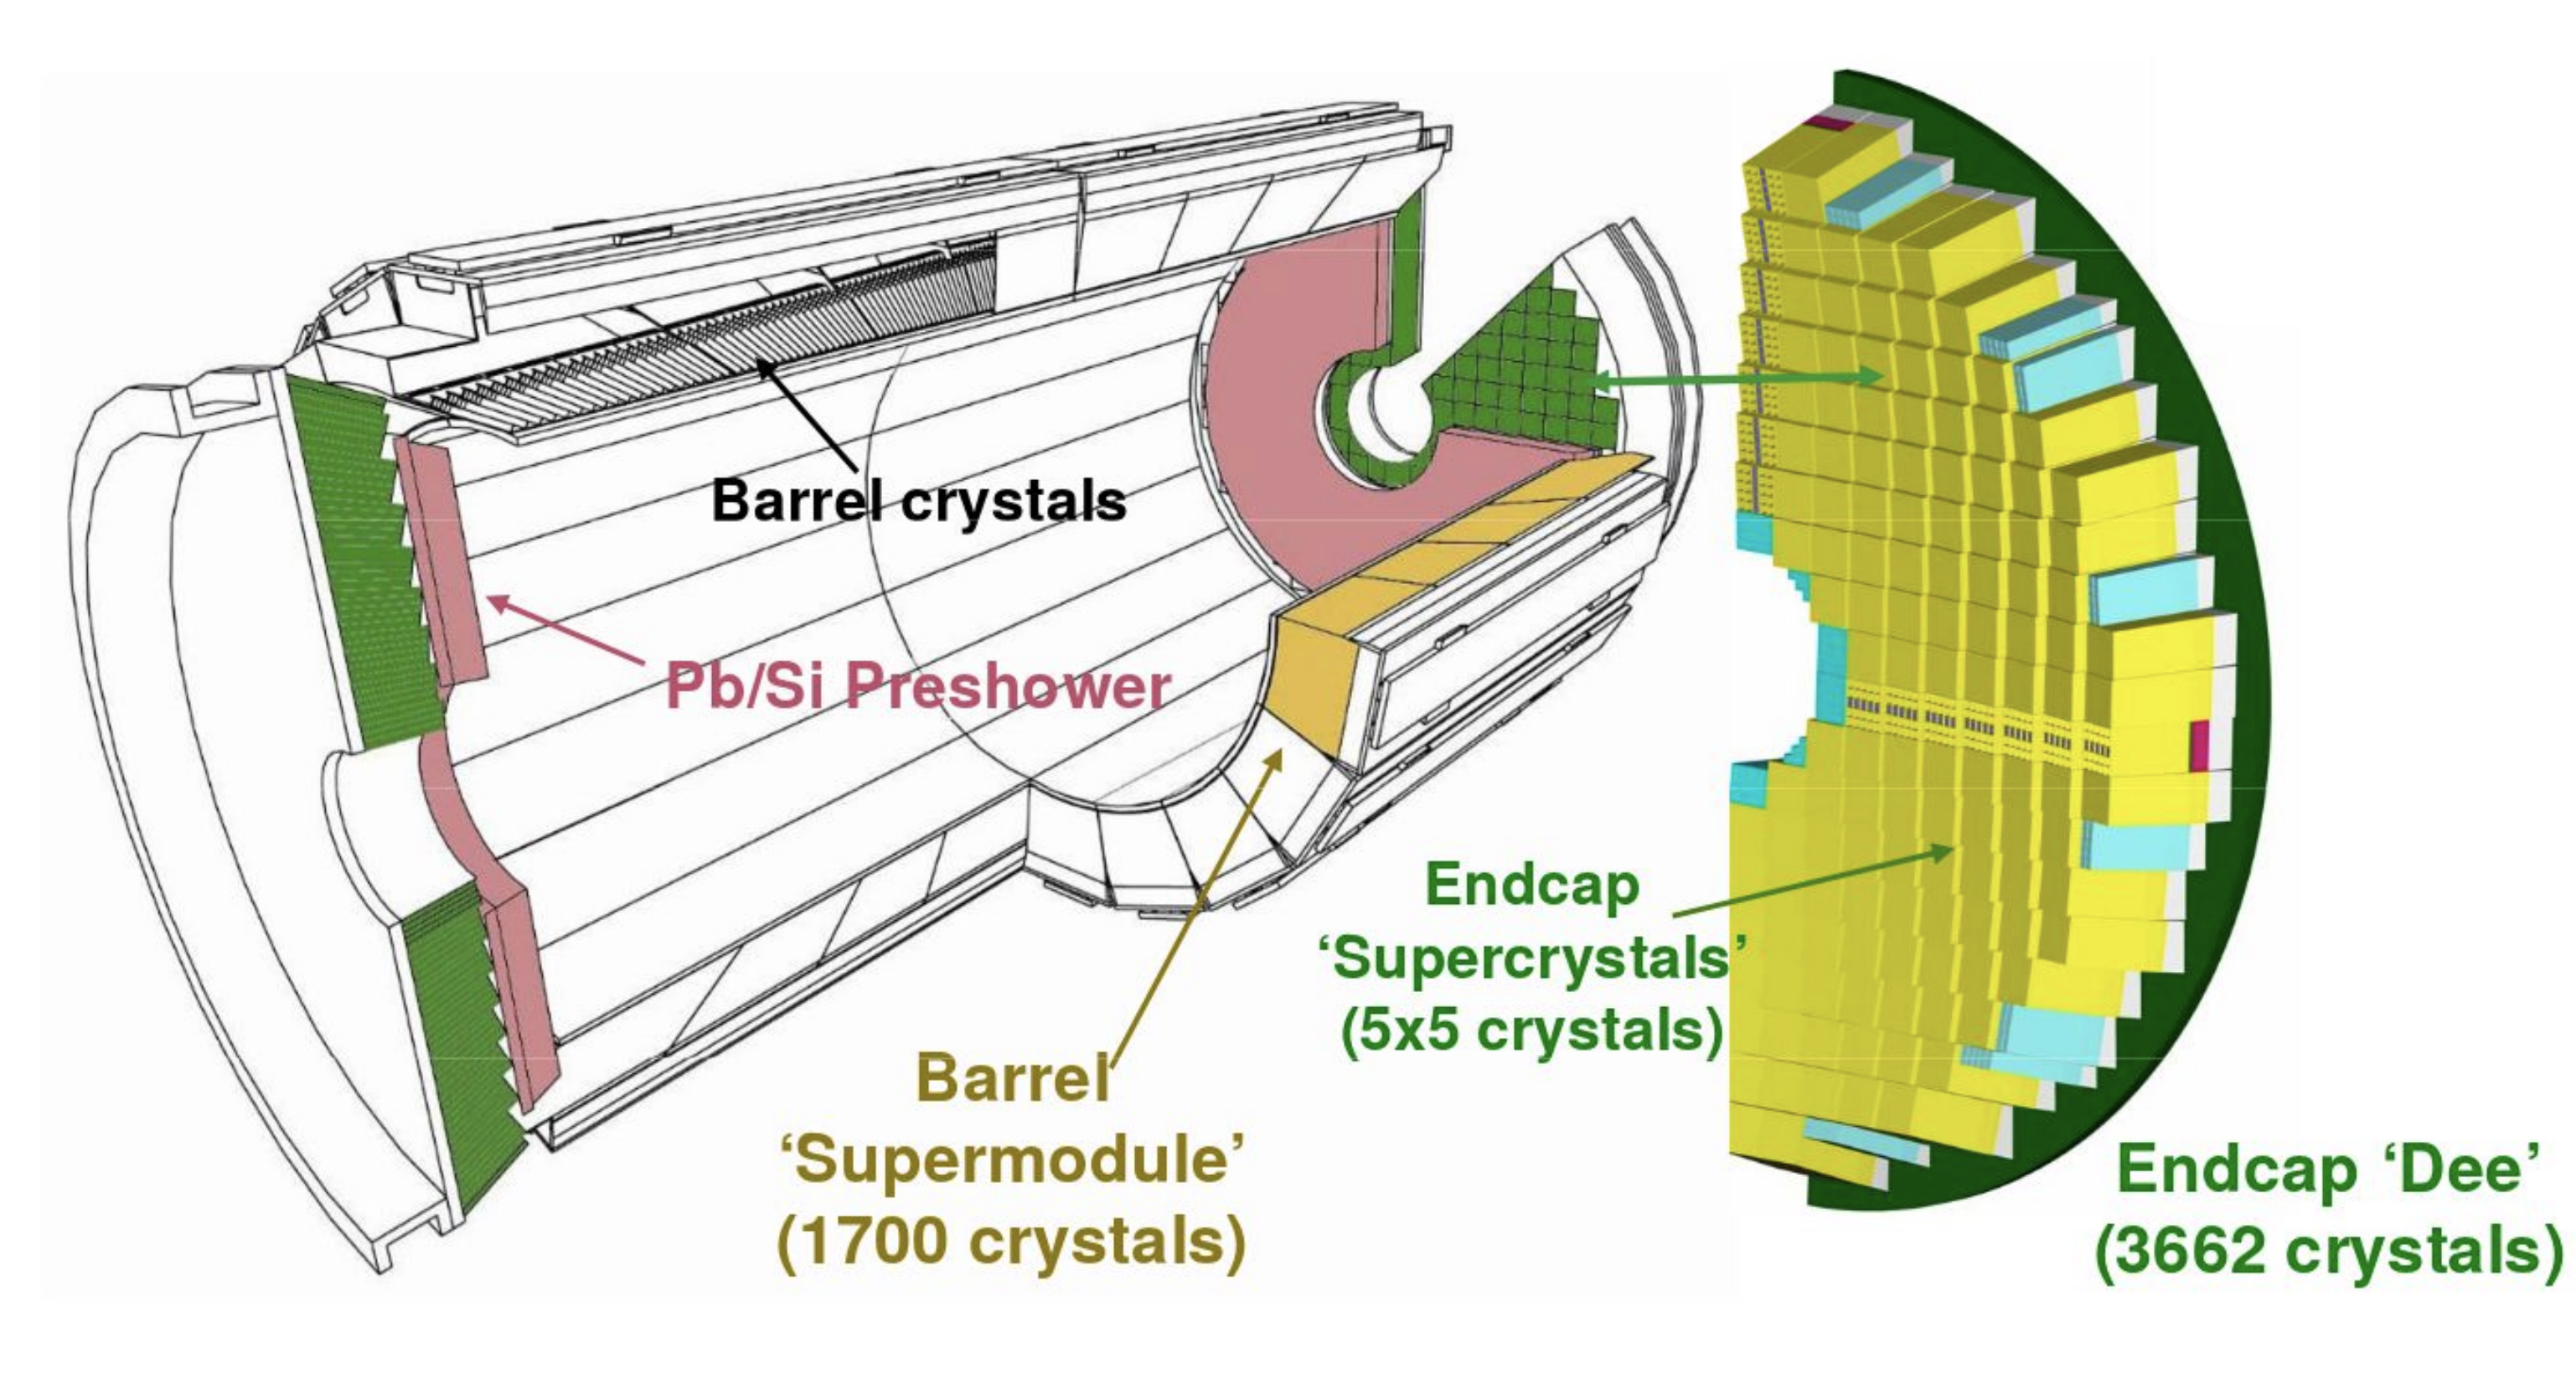
\includegraphics[height=\textwidth]{Images/CMS/ECALDiagram2.png}
    }
    \caption{Left: A photograph of an ECAL crystal. Right: A cutaway showing the orientation of the ECAL supermodules in the barrel and endcap.}
    \label{fig:ECAL}
\end{figure}

\begin{figure}[H]
    \centering
    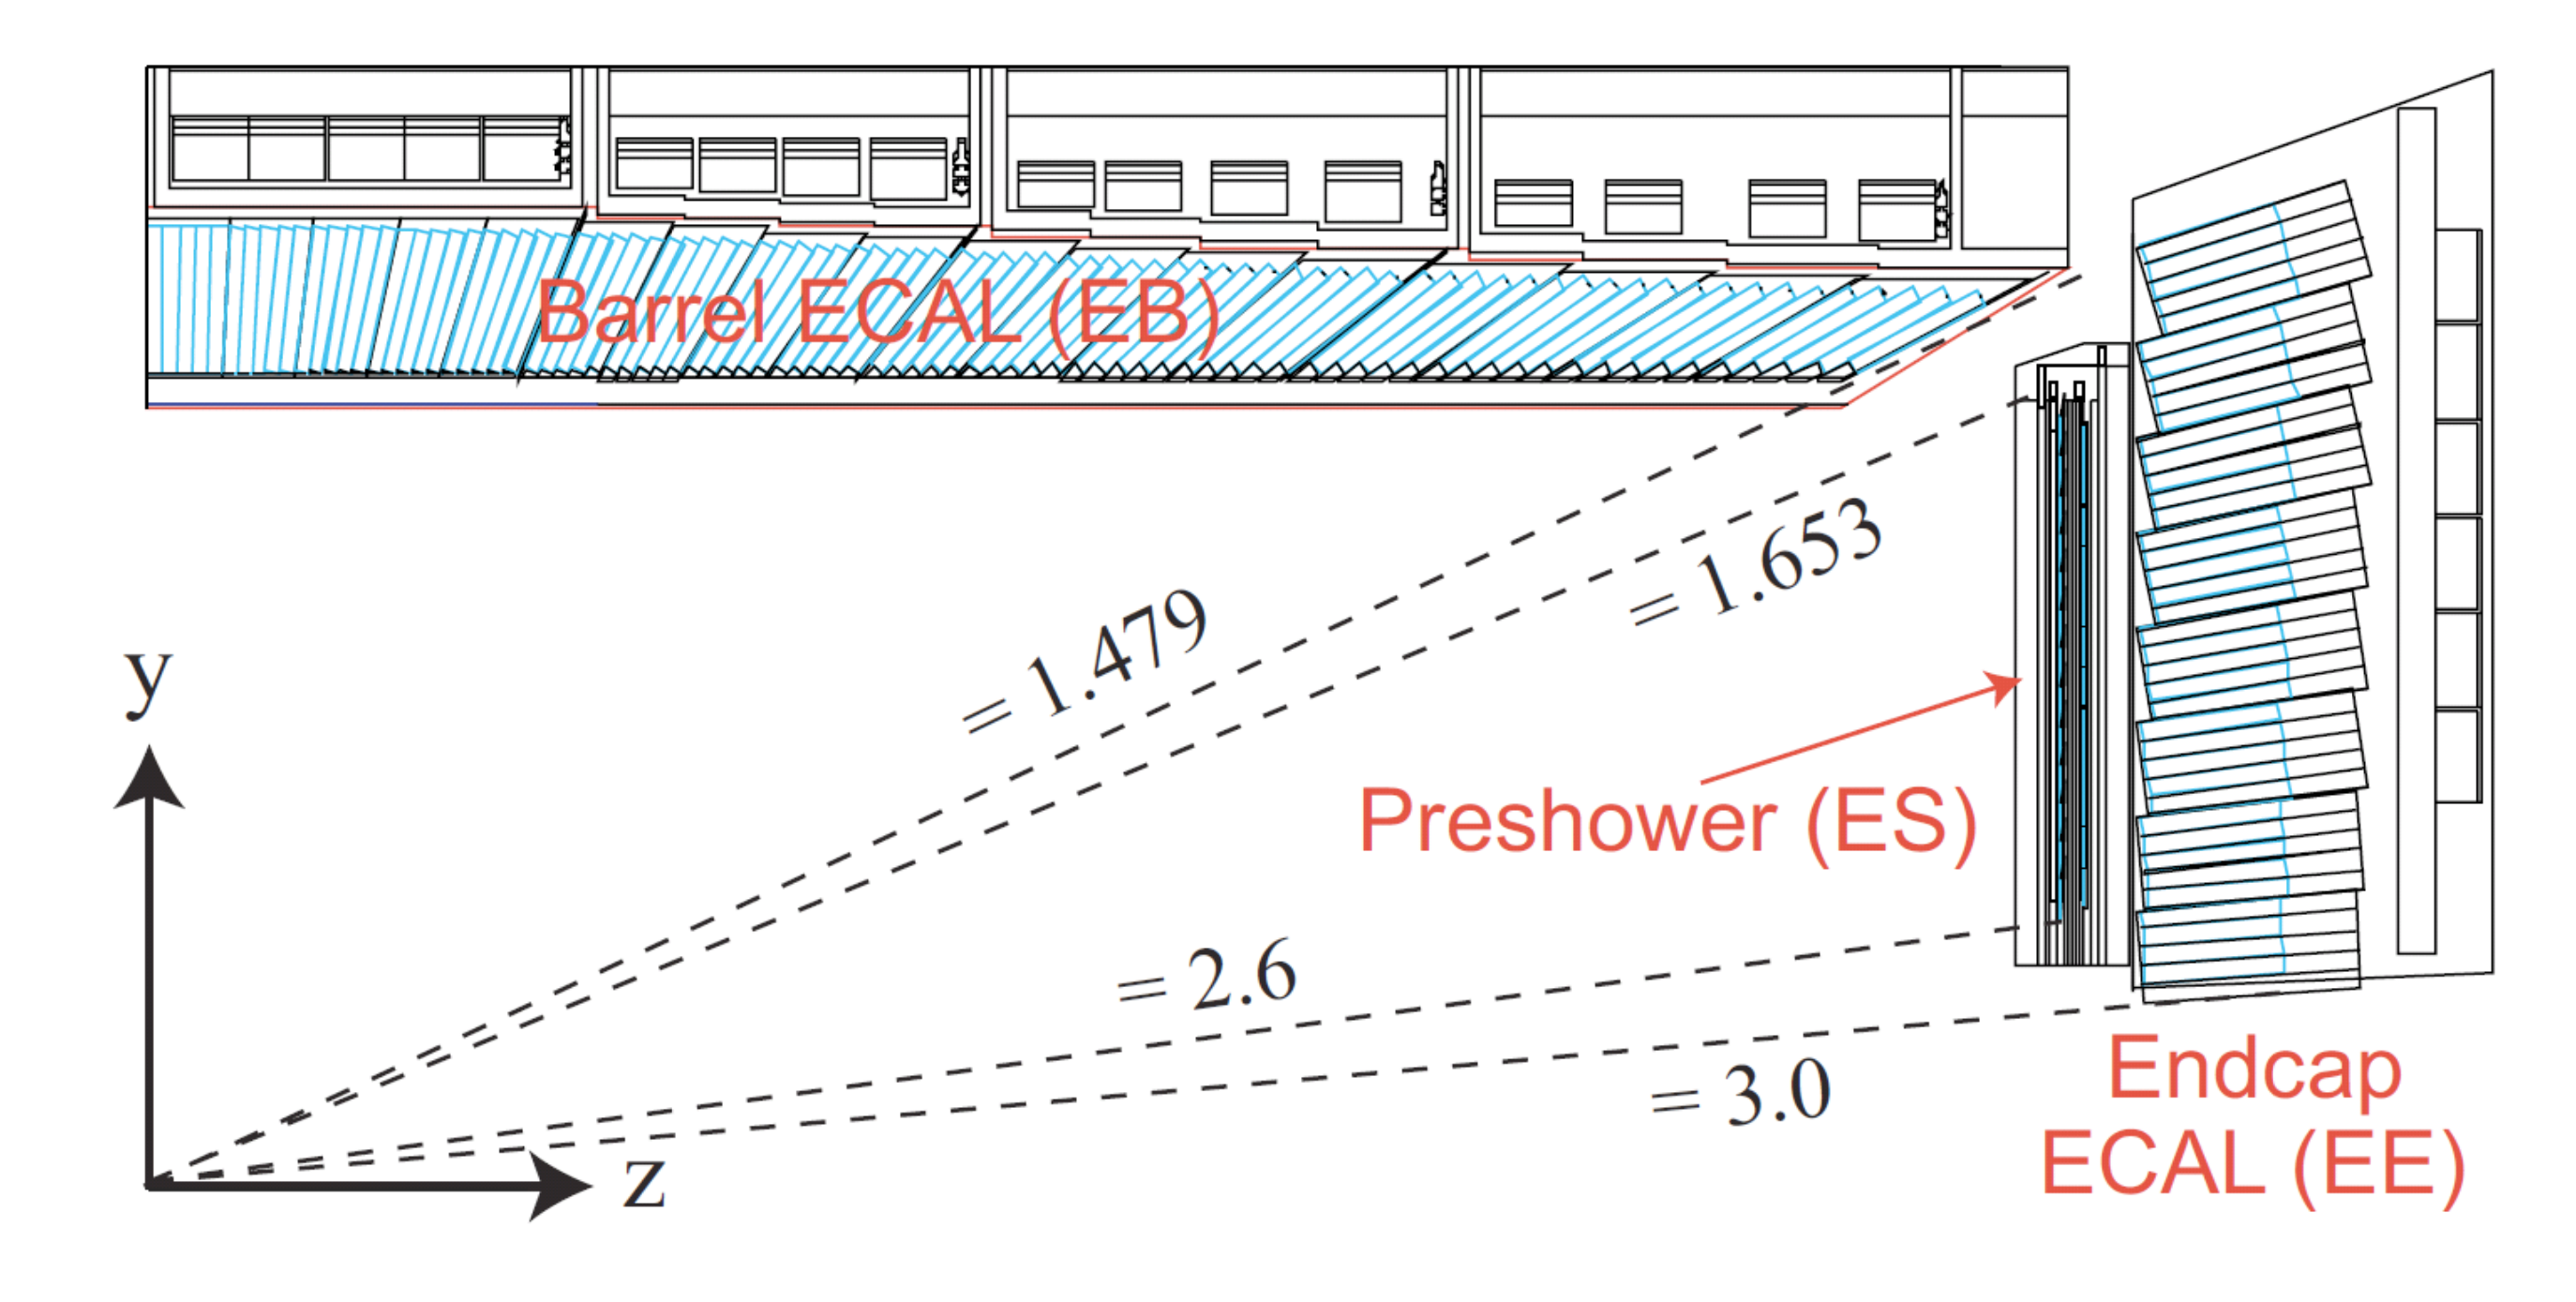
\includegraphics[width=\textwidth]{Images/CMS/ECALDiagram.png}
    \caption{A schematic cutaway showing one quadrant of the ECAL.}
    \label{fig:ECALDiagram}
\end{figure}

\subsubsection{The Hadron Calorimeter} \label{sec:HCAL}
% Introduce detector, location, basic info (e.g., chamber count)
% What is the technology
% Anatomy of a chamber
% How are they arranged in the barrel/endcap
% What do they measure
% Coverage
% Performance

The CMS Hadron Calorimeter (HCAL) \cite{HCALTDR} measures quark, gluon, and neutral particle energy and direction by observing jet energy and missing transverse energy. Within the solenoid magnet, the HCAL is separated into a barrel (HB) and two endcaps (HE), forming the ``central'' HCAL, with a combined pseudorapidity coverage of $|\eta| < 3.0$. An additional two detectors are located outside the solenoid magnet: an array of scintilators that catch the tails of hadronic showers and aid in muon identification called the HCAL Outer calorimeter (HO); and the forward calorimeter (HF), located \SI{6}{m} down the beamline from the ``central'' HCAL (one at each end) and covering the pseudorapidity range $3.0<|\eta|<5.0$, required for accurate missing transverse energy measurements (a diagram showing the arrangement and pseudorapidity coverage of the HCAL and HF is shown in Fig.~\ref{fig:HCALDiagram}). The HB is divided into two half-barrels, each housing 18 wedges ($20^{\circ}$ in $\phi$) of brass alloy absorber plates with a wavelength shifting fiber (WSF) readout. Both the HEs and HFs are composed of quartz fibers embedded in a copper absorber matrix. Optical signals are transmitted to hybrid photo diodes (HPD) in the HB and HE, and by photomultiplier tubes (PMT) in the HFs. A photograph of the HB during installation is shown in Fig.~\ref{fig:HCAL}.

\begin{figure}[H]
    \centering
    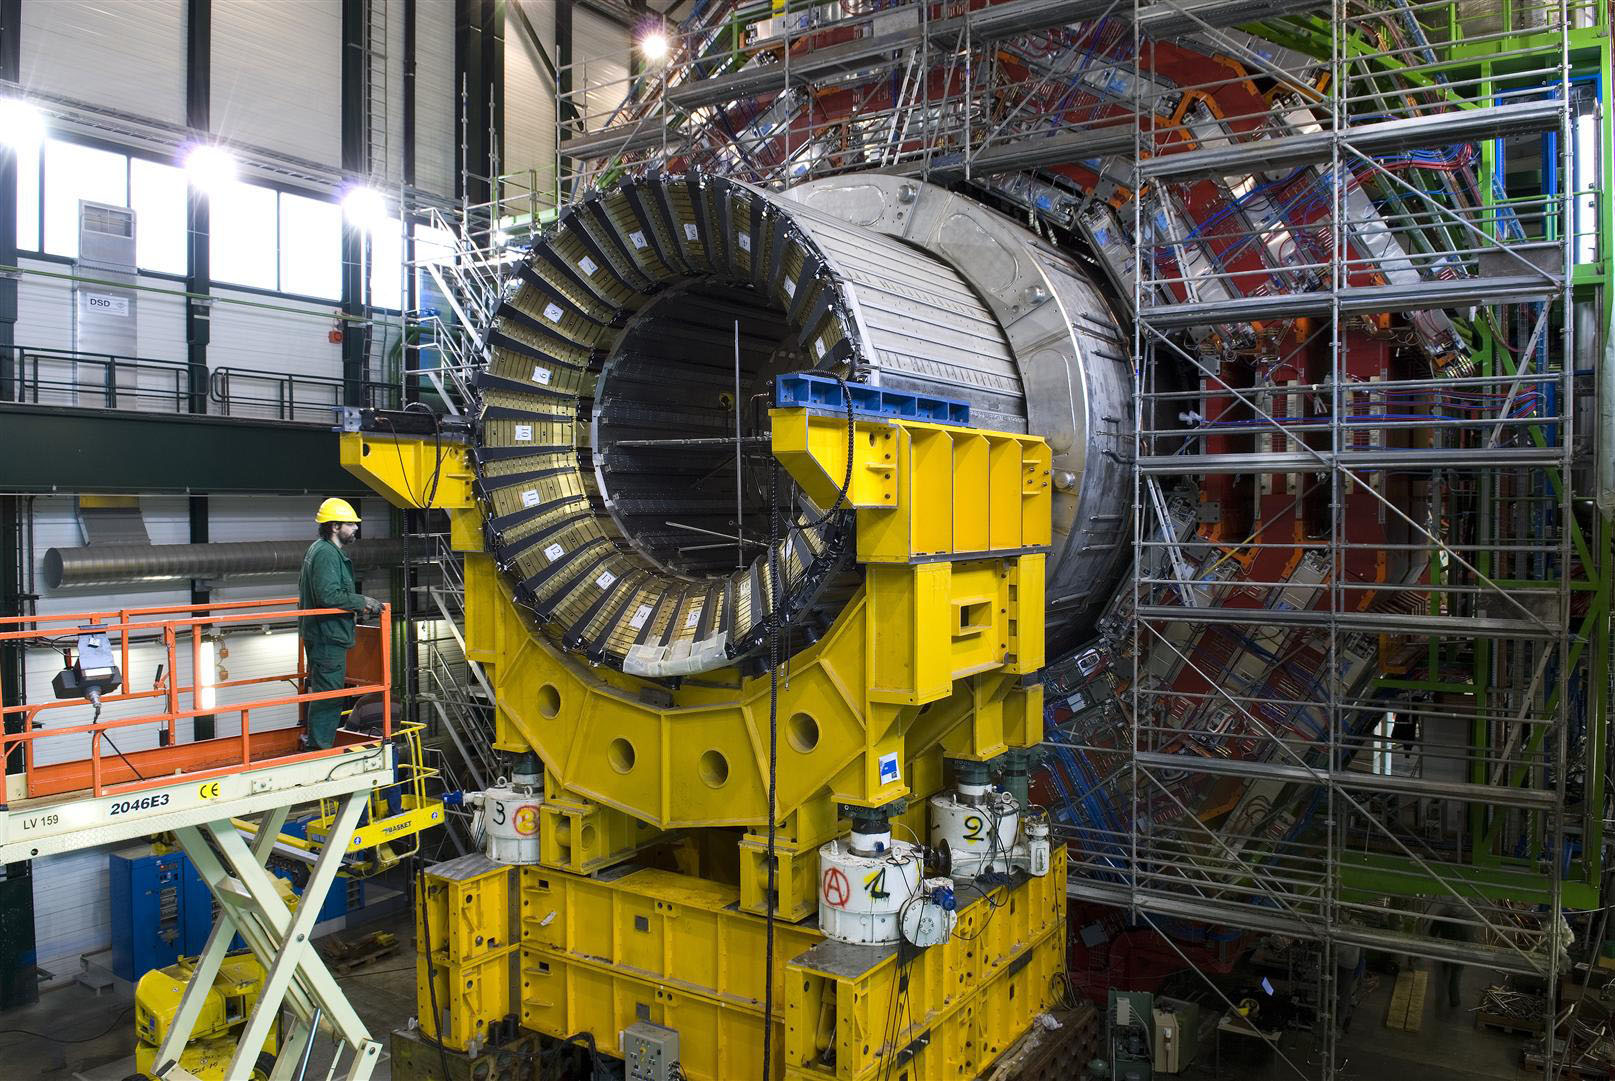
\includegraphics[width=\textwidth]{Images/CMS/HCal.jpg}
    \caption{A photograph showing the HCAL barrel during installation.}
    \label{fig:HCAL}
\end{figure}

\begin{figure}[H]
    \centering
    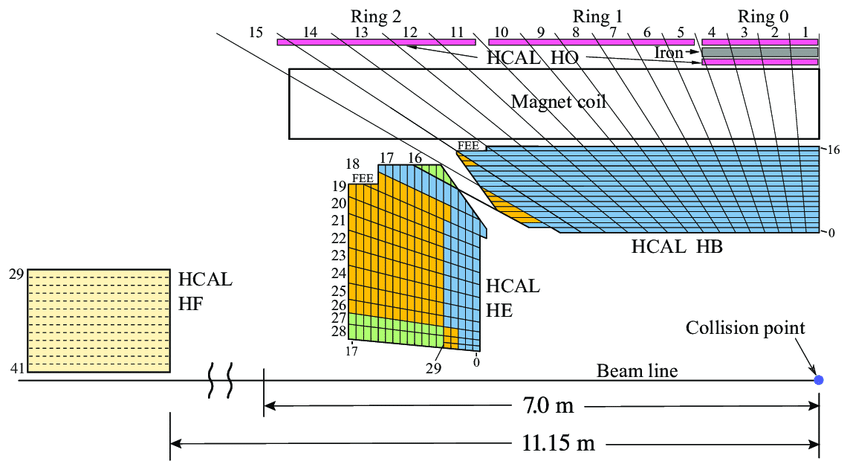
\includegraphics[width=\textwidth]{Images/CMS/HCALDiagram.png}
    \caption{A schematic cutaway showing one quadrant of the HCAL.}
    \label{fig:HCALDiagram}
\end{figure}

\subsection{Solenoid magnet} \label{sec:SolenoidMagnet}


Enclosing the CMS tracker and calorimeters is a \SI{3.8}{T} superconducting solenoid magnet---the most powerful in the world. The cylindrical structure of the solenoid measures \SI{6}{m} in internal diameter and \SI{12.5}{m} long, seen in the photograph in Fig.~\ref{fig:Magnet}. The high magnetic field inside the solenoid is necessary to induce sufficient bending of charged particle trajectories in the transverse plane so precise $p_T$ measurements can be made by the tracker. Outside the solenoid is a ferromagnetic return yoke made of construction steel, divided into five wheels in the barrel region labeled YBw and three disks n in each (positive and negative) endcap labeled YE$\pm$n. The return yoke induces a strong magnetic field within the muon system (mounted to the return yoke) that improves the $p_T$ measurements of muons. The direction of the bending of particles inside the tracker and muon systems is also used to identify the charge sign. The solenoid magnet also serves as a support structure for the \SI{10000}{ton} steel return yoke.

\begin{figure}[H]
    \centering
    {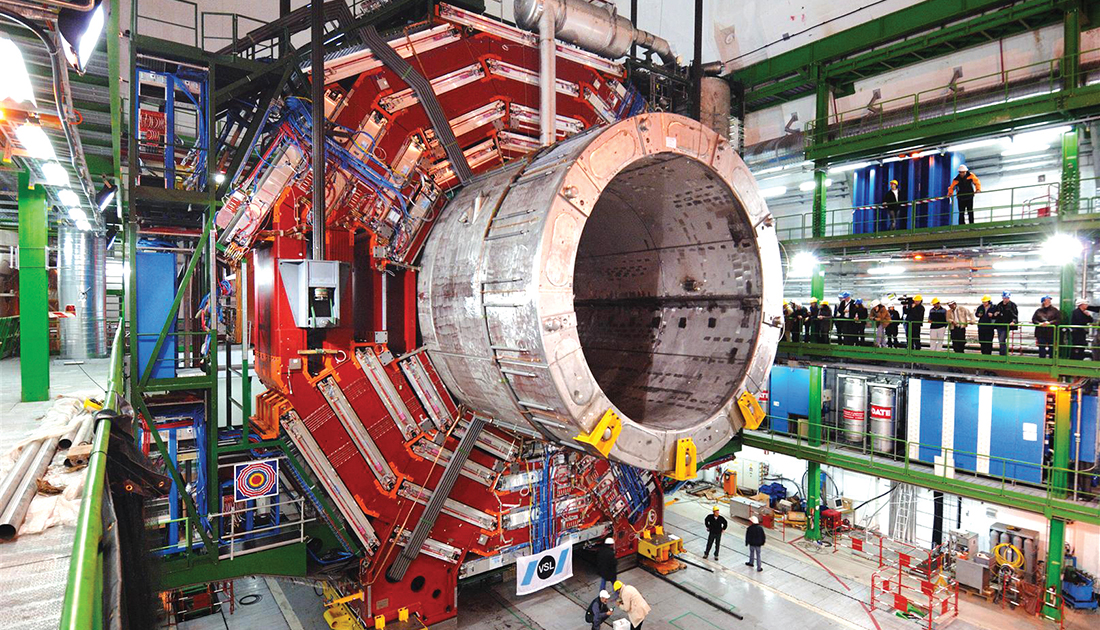
\includegraphics[width=\textwidth]{Images/CMS/Magnet.jpg}}
    \caption{The solenoid magnet of CMS together with a wheel of the steel return yoke.}
    \label{fig:Magnet}
\end{figure}


\subsection{Muon system} \label{sec:MuonSystem}
The muon system \cite{MuonTDR} is responsible for recording the momenta of muons in the outer-most layer of CMS. As muons provide a clean signature in many physics analyses, obtaining high-resolution measurements of muon momenta is critical. It comprises four separate technologies that provide redundancy in both the barrel and endcap regions. The subsystems are the Drift Tubes (DTs) in the barrel, the Cathode Strip Chambers (CSCs) in the endcap regions, the Resistive Plate Chambers (RPCs) in both the barrel and endcaps, and as of Run 3, the Gas Electon Multipliers (GEMs) located in the outer-most layer of the endcaps. Each subsytem uses a different technology and records muon hits separately, with reconstruction combining the information from all the subsystems. The muon barrel (MB) system is divided into four concentric shells, or stations, in each of the five wheels of the CMS barrel, labeled from inner-most to outer-most (along the $r$-coordinate): MB1, MB2, MB3, and MB4. Similarly, the muon endcap (ME) system is arranged into four disks in both the plus and minus endcaps, also called stations, labeled from inner-most to outer-most (along the $z$-coordinate): ME$\pm$1, ME$\pm$2, ME$\pm$3, and ME$\pm$4 ($\pm$ of course identifies the plus or minus endcap). Figure~\ref{fig:MuonSystem} shows a diagram including each subsytem and the pseudorapidity coverage of the muon system.

\begin{figure}[H]
    \centering
    {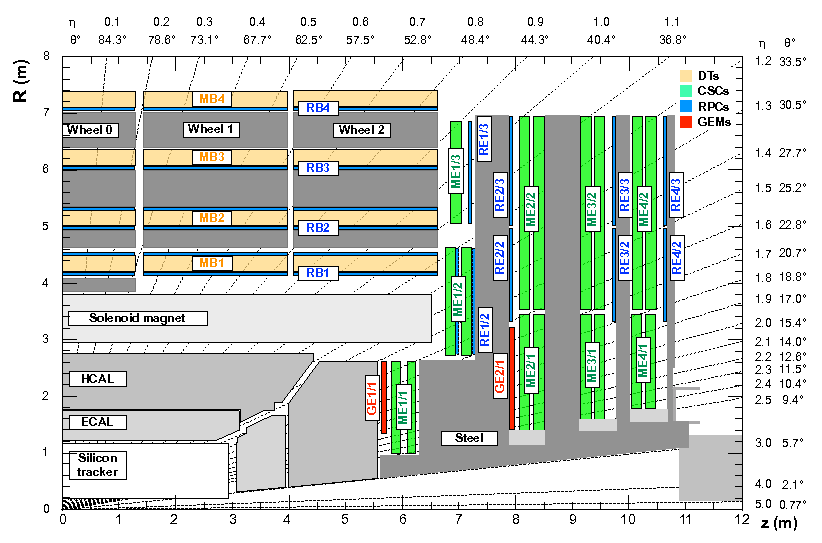
\includegraphics[width=1\textwidth]{Images/CMS/MuonSystem.png}}
    \caption{A cutaway schematic of one quadrant of the muon system. Included are the CSCs, DT chambers, RPCs, and GEM detectors.}
    \label{fig:MuonSystem}
\end{figure}

\subsubsection{Cathode Strip Chambers} \label{sec:CSC}
\input{Text/Chapters/Experiment/Sections/CMS/MuonSystem/CSC}

\subsubsection{Drift Tubes} \label{sec:DT}
\input{Text/Chapters/Experiment/Sections/CMS/MuonSystem/DT}

\subsubsection{Resistive Plate Chambers} \label{sec:RPC}
\input{Text/Chapters/Experiment/Sections/CMS/MuonSystem/RPC}

\subsubsection{Gas Electron Multipliers} \label{sec:GEM}
\input{Text/Chapters/Experiment/Sections/CMS/MuonSystem/GEM} 

\subsection{Trigger system} \label{sec:Trigger}

At the LHC's design luminosity, bunch crossings occur every \SI{25}{ns}. Most of these collisions result in low-energy multi-jet events with little potential for new physics searches. More rare are interesting physics events with smaller cross-sections (e.g., single- and pair-production of heavy bosons, top-antitop creation, digamma events, etc.), however, offline storage capacity limits the fraction of these events that can be kept. This requires CMS to include a fast trigger system \cite{Trigger} to identify events of potential interest with clean, high-quality particle signatures. The CMS trigger system is two-tiered: a low-level trigger built from custom-designed electronics and a high-level trigger that runs reconstruction and selection algorithms on comercial PCs.

\subsubsection{Level one trigger} \label{sec:L1Trigger}

The CMS Level-1 (L1) trigger makes the initial event selection to reduce the \SI{40}{MHz} collision rate. Both the muon system and the calorimeters separately generate packets of coarse-grain spatial and kinematic information of particle-candiates called trigger primitives (TPs). The L1 muon trigger is segmented into three regional track finders: the barrel muon track finder (BMTF), the overlap muon track finder (OMTF), and the endcap muon track finder (EMTF). Each muon subdetector (CSCs, DTs, and RPCs) passes hit information in the form of TPs carrying position, direction, and timing information to the regional track finders. The track finders then  separately reconstruct muon tracks and send that information to the Global Muon Trigger (GMT) which eliminates any redundant tracks based off $p_T$ and quality. The L1 calorimeter trigger combines TPs carrying energy information from the ECAL, HCAL, and HF. In the EB, a five-by-five array of ECAL crystals are combined into a trigger tower (TT), whose transverse energy sum forms a single TP (similarly in the EE, where TTs may have 5-25 crystals). Trigger Concentrator Cards (TCCs) collect TPs from the ECAL and HCAL and form electron, photon, jet, and hadronically-decaying tau candidates before they are combined in the Global Calorimeter Trigger (GCT). Reconstructed L1 trigger objects form the GMT and GCT are merged in the Global Trigger (GT), where they are compared to a ``menu'' of up to 128 algorithms (refered to as ``seeds''). If an event satisfies the criteria of at least one seed, an L1 accept (L1A) is sent upstream to the subdetectors. Upon reciept of an L1A, TPs and all detector information from the data aquisition (DAQ) system---stored in the buffers of onboard electronics---are sent downstream to be processed by the high-level trigger. The latency of the L1 trigger is fixed at approximately \SI{4}{\micro s}, a requirement set by the collision rate and the buffer sizes of the different subsytems, and sustains an output rate of \SI{100}{kHz}. A flow chart of the L1 trigger system is shown in Fig.~\ref{fig:L1TriggerMap}.

\begin{figure}[H]
    \centering
    {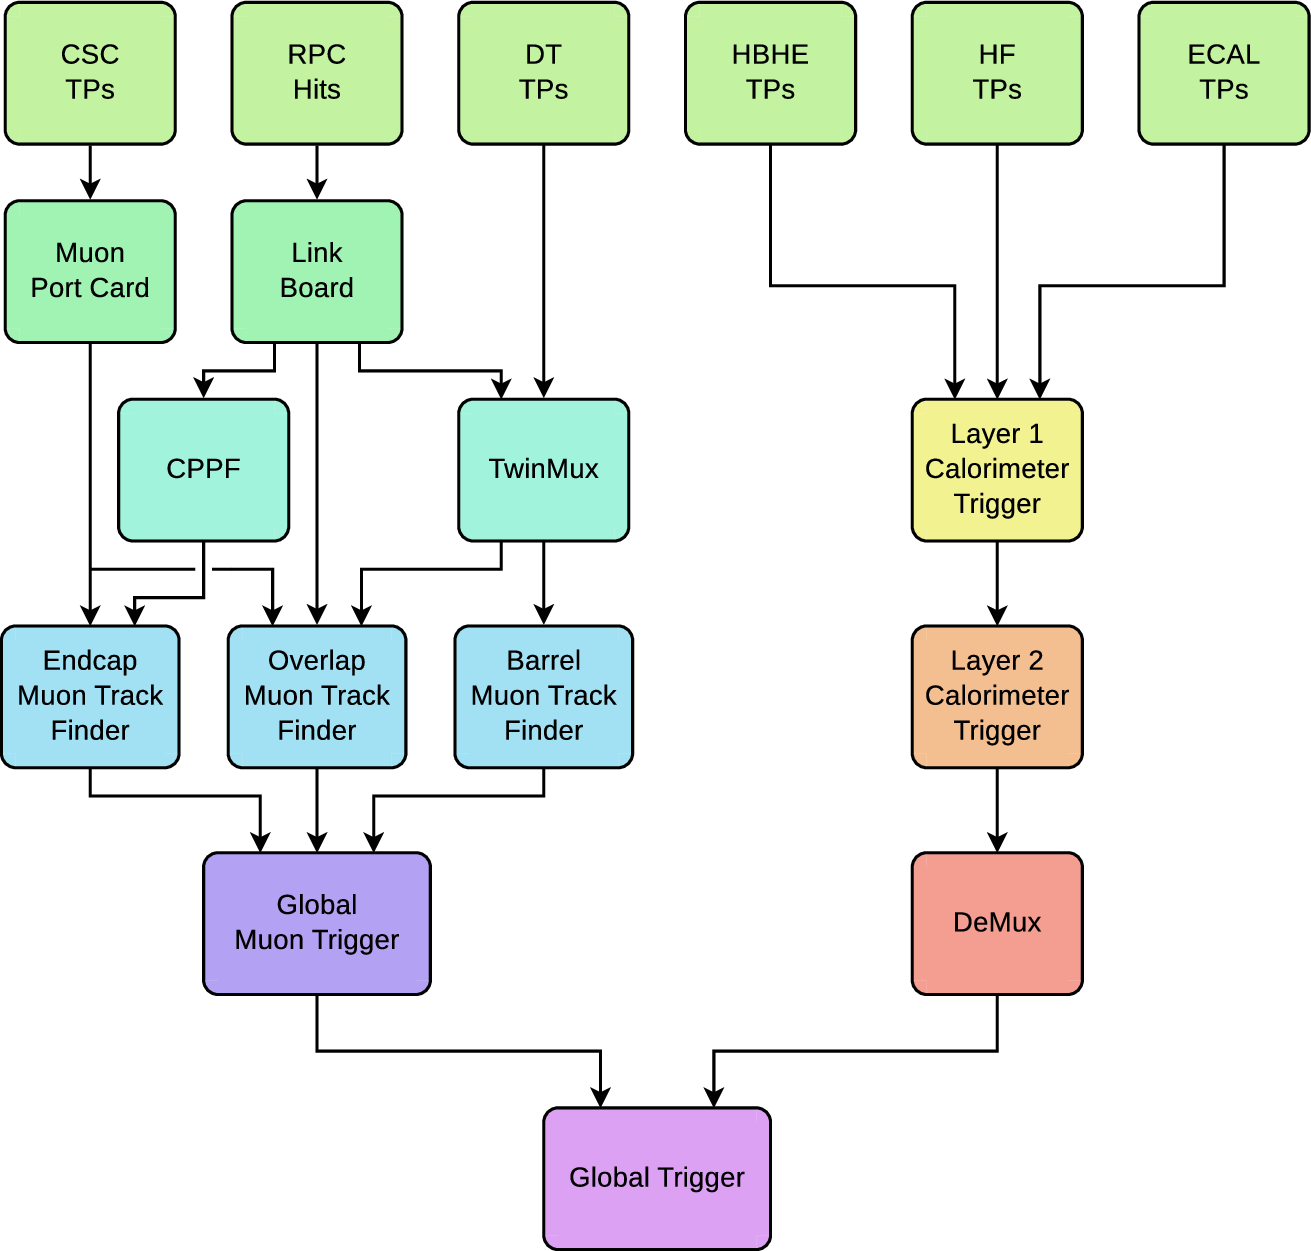
\includegraphics[width=\textwidth]{Images/CMS/L1TriggerMap.png}}
    \caption{A flow chart of the CMS L1 trigger system.}
    \label{fig:L1TriggerMap}
\end{figure}

\subsubsection{High-level trigger} \label{sec:HLT}
To further reduce the L1A output rate, the high-level trigger (HLT) makes a final selection of events with a \SI{1}{kHz} readout rate, acceptable for offline reconstruction and permanent storage. Implemented in software running on a farm of commercial computers, the HLT takes an L1A seed and performs a streamlined reconstruction with a similar efficiency to that used in offline processing. The HLT then filters events in roughly two stages: first, using only muon system and calorimeter information, and second, using full tracks. Events selected by the HLT algorithms are sent to permanent storage. A photograph of a GPU used to process the HLT algorithms is shown in Fig.~\ref{fig:HLTGPU}.

\begin{figure}[H]
    \centering
    {\includegraphics[width=\textwidth]{Images/CMS/HLTGPU.png}}
    \caption{A GPU used to process the HLT algorithms.}
    \label{fig:HLTGPU}
\end{figure}

\chapter{Phase II upgrades} \label{chapter:Phase2Upgrades}
\section{High-Luminosity LHC} \label{sec:HLLHC}
Since its commisioning in 2010, the LHC has provided experiments like CMS the opportunity to test the SM with astonishing precision. Using data collected in Runs 1 and 2, the LHC experiments have had a prolific 13 years of scientific study, boasting a combined total of roughly 3000 publications in refereed journals, with CMS contributing over 1000 physics papers to that total. Even still, theories of physics beyond the SM remain undiscovered at the LHC, with questions of Supersymmetry, Dark Matter, Grand Unification left on the table. To heighten the sensitivity of new physics searches and expand the scope of the LHC physics program, a significant upgrade to the collider is planned that will increase the integrated luminosity by a factor of ten beyond the original design. The High-Luminosity LHC (HL-LHC) is slated to begin proton-proton collisions in 2029 with the start of Run 4, kicking off Phase-2 of data-taking. Infrastructure work for the HL-LHC concluded during LS2, making way for construction of the machine in LS3 including upgrades to the quadruple magnets, cryogenics, and collimators. In addition to increased luminosity, the HL-LHC will boost the proton-proton collision energies to \SI{14}{TeV}. 

Over the next two decades, the HL-LHC is expected to deliver an integrated luminosity of \SI{3000}{\fbinv}, overshadowing the projected \SI{350}{\fbinv} for Phase-1. To accumulate this much data, the collision rate inside CMS will have to be much higher than in Phase-1, which will necessarily present challenges to each subsystem. Inside CMS, the number of overlapping secondary collisions coinciding with the primary interaction, called Pile-Up (PU), averaged about 30 interactions per bunch crossing in Run 2. Specialized algorithms, such as Pile-Up Per Particle Identification (PUPPI), are used to mitigate the effects of PU. At the HL-LHC, PU within CMS may reach up to 200 interactions per bunch crossing. To reject the abundance of unwanted particles recorded in these high-PU events will require the development of more sophisticated filtering techniques and higher granularity detectors. An event display showcasing the sheer volume of particle tracks within CMS of a high-PU event can be found in Fig.~\ref{fig:highPU}. 

\begin{figure}[H]
    \centering
    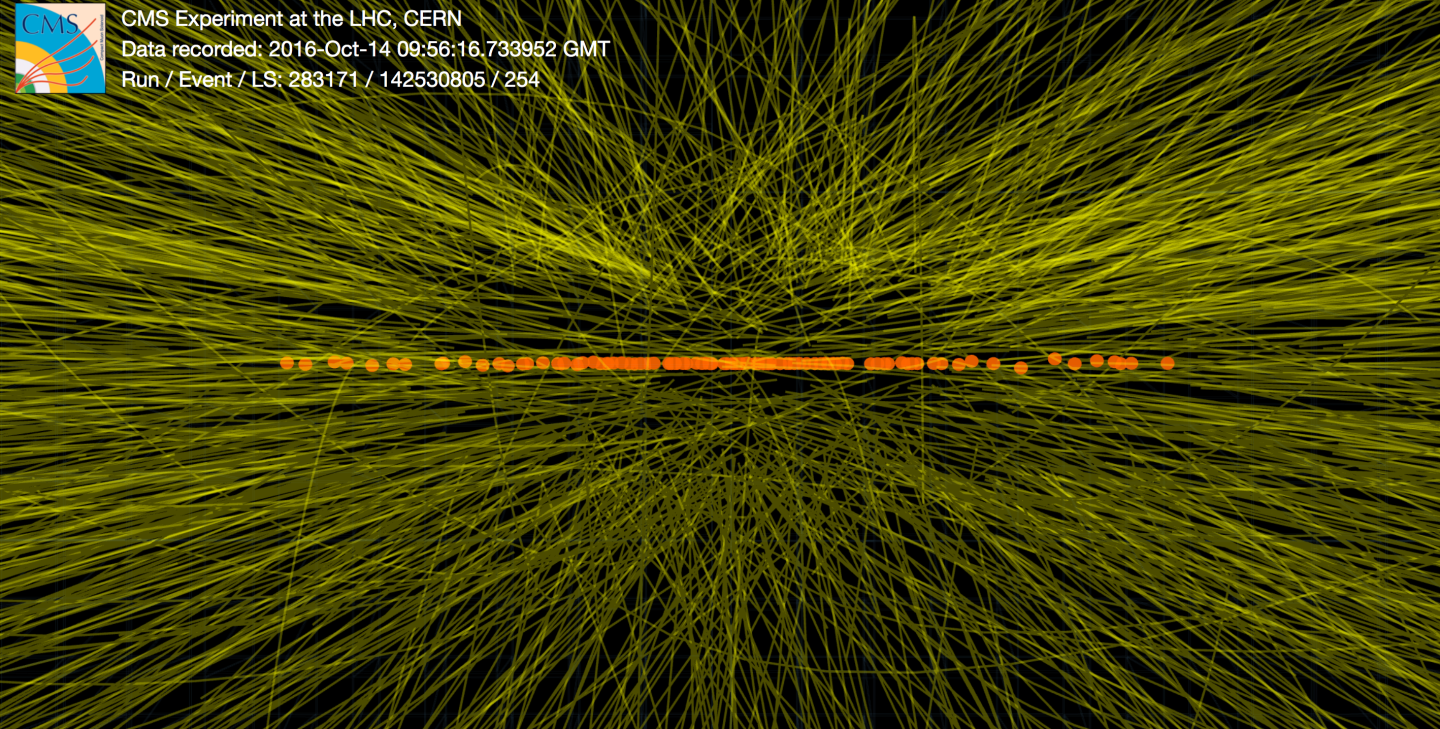
\includegraphics[width=1\textwidth]{Images/Phase2Upgrades/highpileup.png}
    \caption{An event display of a 130 PU event recorded by CMS.}
    \label{fig:highPU}
\end{figure}

The environment inside the detector throughout Phase-2 will place additional performance demands on CMS. The increase in particle flux will rapidly age current detector components, especially close to the beam pipe. Improved radiation hardness, especially of front-end detector electronics, will be required to withstand the harsh conditions. Furthermore, limited data readout bandwidth coupled with the current L1 trigger rate and latency will prove insufficient to handle the expected occupancies in Phase-2, resulting in unacceptable data loss. To cope with the challenges presented in Phase-2 of running, while profiting from the increase in luminosity, an extensive program of upgrades to the CMS subsystems was prepared and will be fully integrated prior to the first HL-LHC collisions in Run 4.


\section{CSC electronics} \label{sec:CSCElectronics}
\subsection{Phase-1 electronics} \label{sec:Phase1CSCelectronics}

CSC trigger and DAQ channels rely on a sequence of on- and off-chamber electronics for reading, storing, processing, and transmitting the analog signals from the strips and wires. Before explaining the Phase-2 upgrades to the CSCs, a more detailed description of the electronics prior to the upgrades---both on- and off-chamber---is necessary. 

Cathode strip signals are read by five Cathode Front-End Boards (CFEBs) mounted to each CSC (see Fig.~\ref{fig:CFEB}). A number of custom Application Specific Integrated Circuits (ASICs) fused to each CFEB are responsible for shaping, amplifying, and storing cathode strip signals and identifying hits: Buckeye ASICs amplify and shape the signals from each cathode strip before sending signals down trigger and DAQ streams; Comparator ASICs rapidly identify hits with half-strip resolution and send these downstream to an off-chamber Trigger Motherboard (TMB); and Switched Capacitor Arrays (SCAs) store strip charges in anolog form of up to six events while waiting for an L1A from the TMB. Upon reciept of an L1A the SCAs will send precision data to be digitized by Analog-to-Digital Converters (ADCs) before both data and trigger information is forwarded to an off-chamber DAQ Motherboard (DMB). Anode wire signals---``ganged'' into groups of 10-15 wires---are amplified by 42 on-chamber Anode Front-End Boards (AFEBs) and sent to an Anode Local Charged Track (ALCT) board, also on-chamber. A mezzanine on the ALCT baseboard identifies patterns among the anode hits in the six wire layers (a minimum of four layers is consistent with a muon). The two patterns with the most layer hits are sent off-chamber for processing by the TMB. A Low-Voltage Distribution Board (LVDB) on each chamber supplies power to all the electronics.

\begin{figure}[H]
    \centering
    {\includegraphics[width=1\textwidth]{Images/Phase2Upgrades/Electronics/CFEB.png}}
    \caption{One of five CFEBs used to read cathode strip signals on a CSC.}
    \label{fig:CFEB}
\end{figure}

The TMB reads the trigger primitives generated from the on-chamber electronics---Cathode Local Charged Tracks (CLCTs) from the CFEB Comparators and ALCTs from the ALCT board---and from these constructs 2D Local Charged Tracks (LCTs), requiring four layer hits, which are sent to the EMTF. The DMB builds data packets with cathode strip data from the CFEBs, Anode wire data from the ALCT (through the TMB), and trigger data from the TMB. CSC data packets from 15 DMBs corresponding to chambers in a different 20 degree sector in each station (to balance the readout load) are read by Detector Dependent Units (DDUs) with \SI{1.6}{Gb/s} links, unpacked in real-time, then merged and sent to CMS DAQ. DMBs are also responsible for controling on-chamber voltages via the LVMB and controls the CFEBs. Photographs of a TMB and DMB are shown in Fig.~\ref{fig:TMBDMB}.

\begin{figure}[H]
    \centering
    {\includegraphics[width=0.49\textwidth]{Images/Phase2Upgrades/Electronics/TMB.png}}
    {\includegraphics[width=0.49\textwidth]{Images/Phase2Upgrades/Electronics/DMB.png}}
    \caption{Left: A TMB for reading CSC trigger primitives and processing L1As. Right: A DMB for reading and transmitting precision data packets from CSCs.}
    \label{fig:TMBDMB}
\end{figure}

TMBs and DMBs are housed in ``peripheral'' VME crates, each supporting nine CSCs, secured to the edges of each ME disk (six peripheral crates per station). Each peripheral crate also houses the following: a Muon Port Card (MPC) that collects the LCTs from each of the nine TMBs in the crate and sends them to the muon track finder system; A Clock and Control Board (CCB) acting as an interface between the CSCs and the Trigger, Timing and Control (TTC) system of CMS, synchronizing the crate operations; and a VME Crate Controller (VCC) that distributes the VME commands recieved from the control room to the other boards in the peripheral crate.

\subsection{Phase-2 electronics} \label{sec:Phase2CSCelectronics}

Prior to LS1, cathode strips on each ME1/1 chamber had been divided into two groups based on pseudorapidity: ME1/1a covering $2.0 < |\eta|< 2.4$, and ME1/1b covering $1.5 < |\eta| < 2.0$. Issues observed during Run I with muon triggering in the triply-ganged ME1/1a cathode strips required unganging of the strips in all ME1/1 chambers and the a/b division removed. To accomodate the increase in channels and better cope with the trigger rate, ME1/1 chamber electronics underwent several upgrades. The five CFEBs were replaced by seven Digital CFEBs (DCFEBs) to read cathode strip signals. DCFEBs (shown in Fig.~\ref{fig:DCFEB}) continuously digitize strip signals with flash ADCs and store digitized signals in the deep buffers of a Virtex-6 Field Programmable Gate Array (FPGA). Trigger and data readout bandwidth on DCFEBs were upgraded to \SI{3.2}{Gb/s} Finisar optical links. To recieve the optical links from the DCFEBs, the off-chamber TMB/DMB were correspondingly upgraded to an OTMB/ODMB (see Figs.~\ref{fig:OTMB} and~\ref{fig:ODMB})with powerful Virtex-6 FPGAs and \SI{1.6}{Gb/s} output links. The LVDB was upgraded to an LVDB7 and the ALCT mezzanine was upgraded with a Spartan-6 FPGA (ALCT-S6, also ALCT-LX150) capable of improved algorithms for pattern finding. The CFEBs formerly on the ME1/1 chambers were adopted to construct the 72 ME4/2 chambers, which prior to LS1 had not been built due to a lack of funding.

\begin{figure}[H]
    \centering
    {\includegraphics[width=1\textwidth]{Images/Phase2Upgrades/Electronics/DCFEB.png}}
    \caption{DCFEBs used to upgrade the ME1/1 chambers in LS1 and ME234/1 chambers in LS2.}
    \label{fig:DCFEB}
\end{figure}

\begin{figure}[H]
    \centering
    {\includegraphics[width=1\textwidth]{Images/Phase2Upgrades/Electronics/OTMB.png}}
    \caption{Left: an OTMB mezzanine. Right: an OTMB baseboard. The OTMBs replaced the TMBs for ME1/1 chambers in LS1.}
    \label{fig:OTMB}
\end{figure}

\begin{figure}[H]
    \centering
    {\includegraphics[width=1\textwidth]{Images/Phase2Upgrades/Electronics/ODMB.png}}
    \caption{An ODMB used to upgrade the DMBs for ME1/1 chambers in LS1}
    \label{fig:ODMB}
\end{figure}

Radiation tests of CSC modules simulating a decade of HL-LHC data taking revealed that chambers are exceptionally robust, demonstrating adequite performance consitent with Phase-1. Even still, the higher radiation doses anticipated during Phase-2 are expected to cause certain electronic readout components on CSCs at high psuedorapidities to die. Along with mitigating radiation failure, higher PU scenarios will require a faster L1 trigger rate of \SI{750}{Hz} and latency of \SI{12.5}{\micro s}; without remedy, the analog readout of CFEBs on the inner CSC rings would lead to catstrophic event losses, as demonstrated in Fig.~\ref{fig:EventLosses}. To avoid these hazards during Phase-2, CSCs in the inner rings were refurbished with upgrades to their front-end electronics, installed during LS2, with minor upgrades to off-chamber electronics following in LS3. ME1/1 DCFEBs were replaced by more radiation-hard xDCFEBs with improved VTTx/VTRx optical recievers in place of the Finisars (see Fig.~\ref{fig:xDCFEB}). Both the new xDCFEBs and ALCT-LX100s (installed during LS1) provide PROM-less solutions for ME1/1 chambers that mitigate any failures from radiation damage. As for ME234/1 chambers, their ALCTs were upgraded to ALCT-LX150Ts (a picture of the mezzanine is in Fig.~\ref{fig:ALCT}) and their CFEBs were replaced with the disused DCFEBs from the ME1/1 chambers. The Finisar optical transeivers on the DCFEBs were replaced with VTTx links on the ME234/1 chambers to supply sufficient trigger and data readout speeds (\SI{3.2}{Gb/s}). To recieve the now optical trigger links from ME234/1 DCFEBs, TMBs were upgraded to OTMBv2s. 

\begin{figure}[H]
    \centering
    {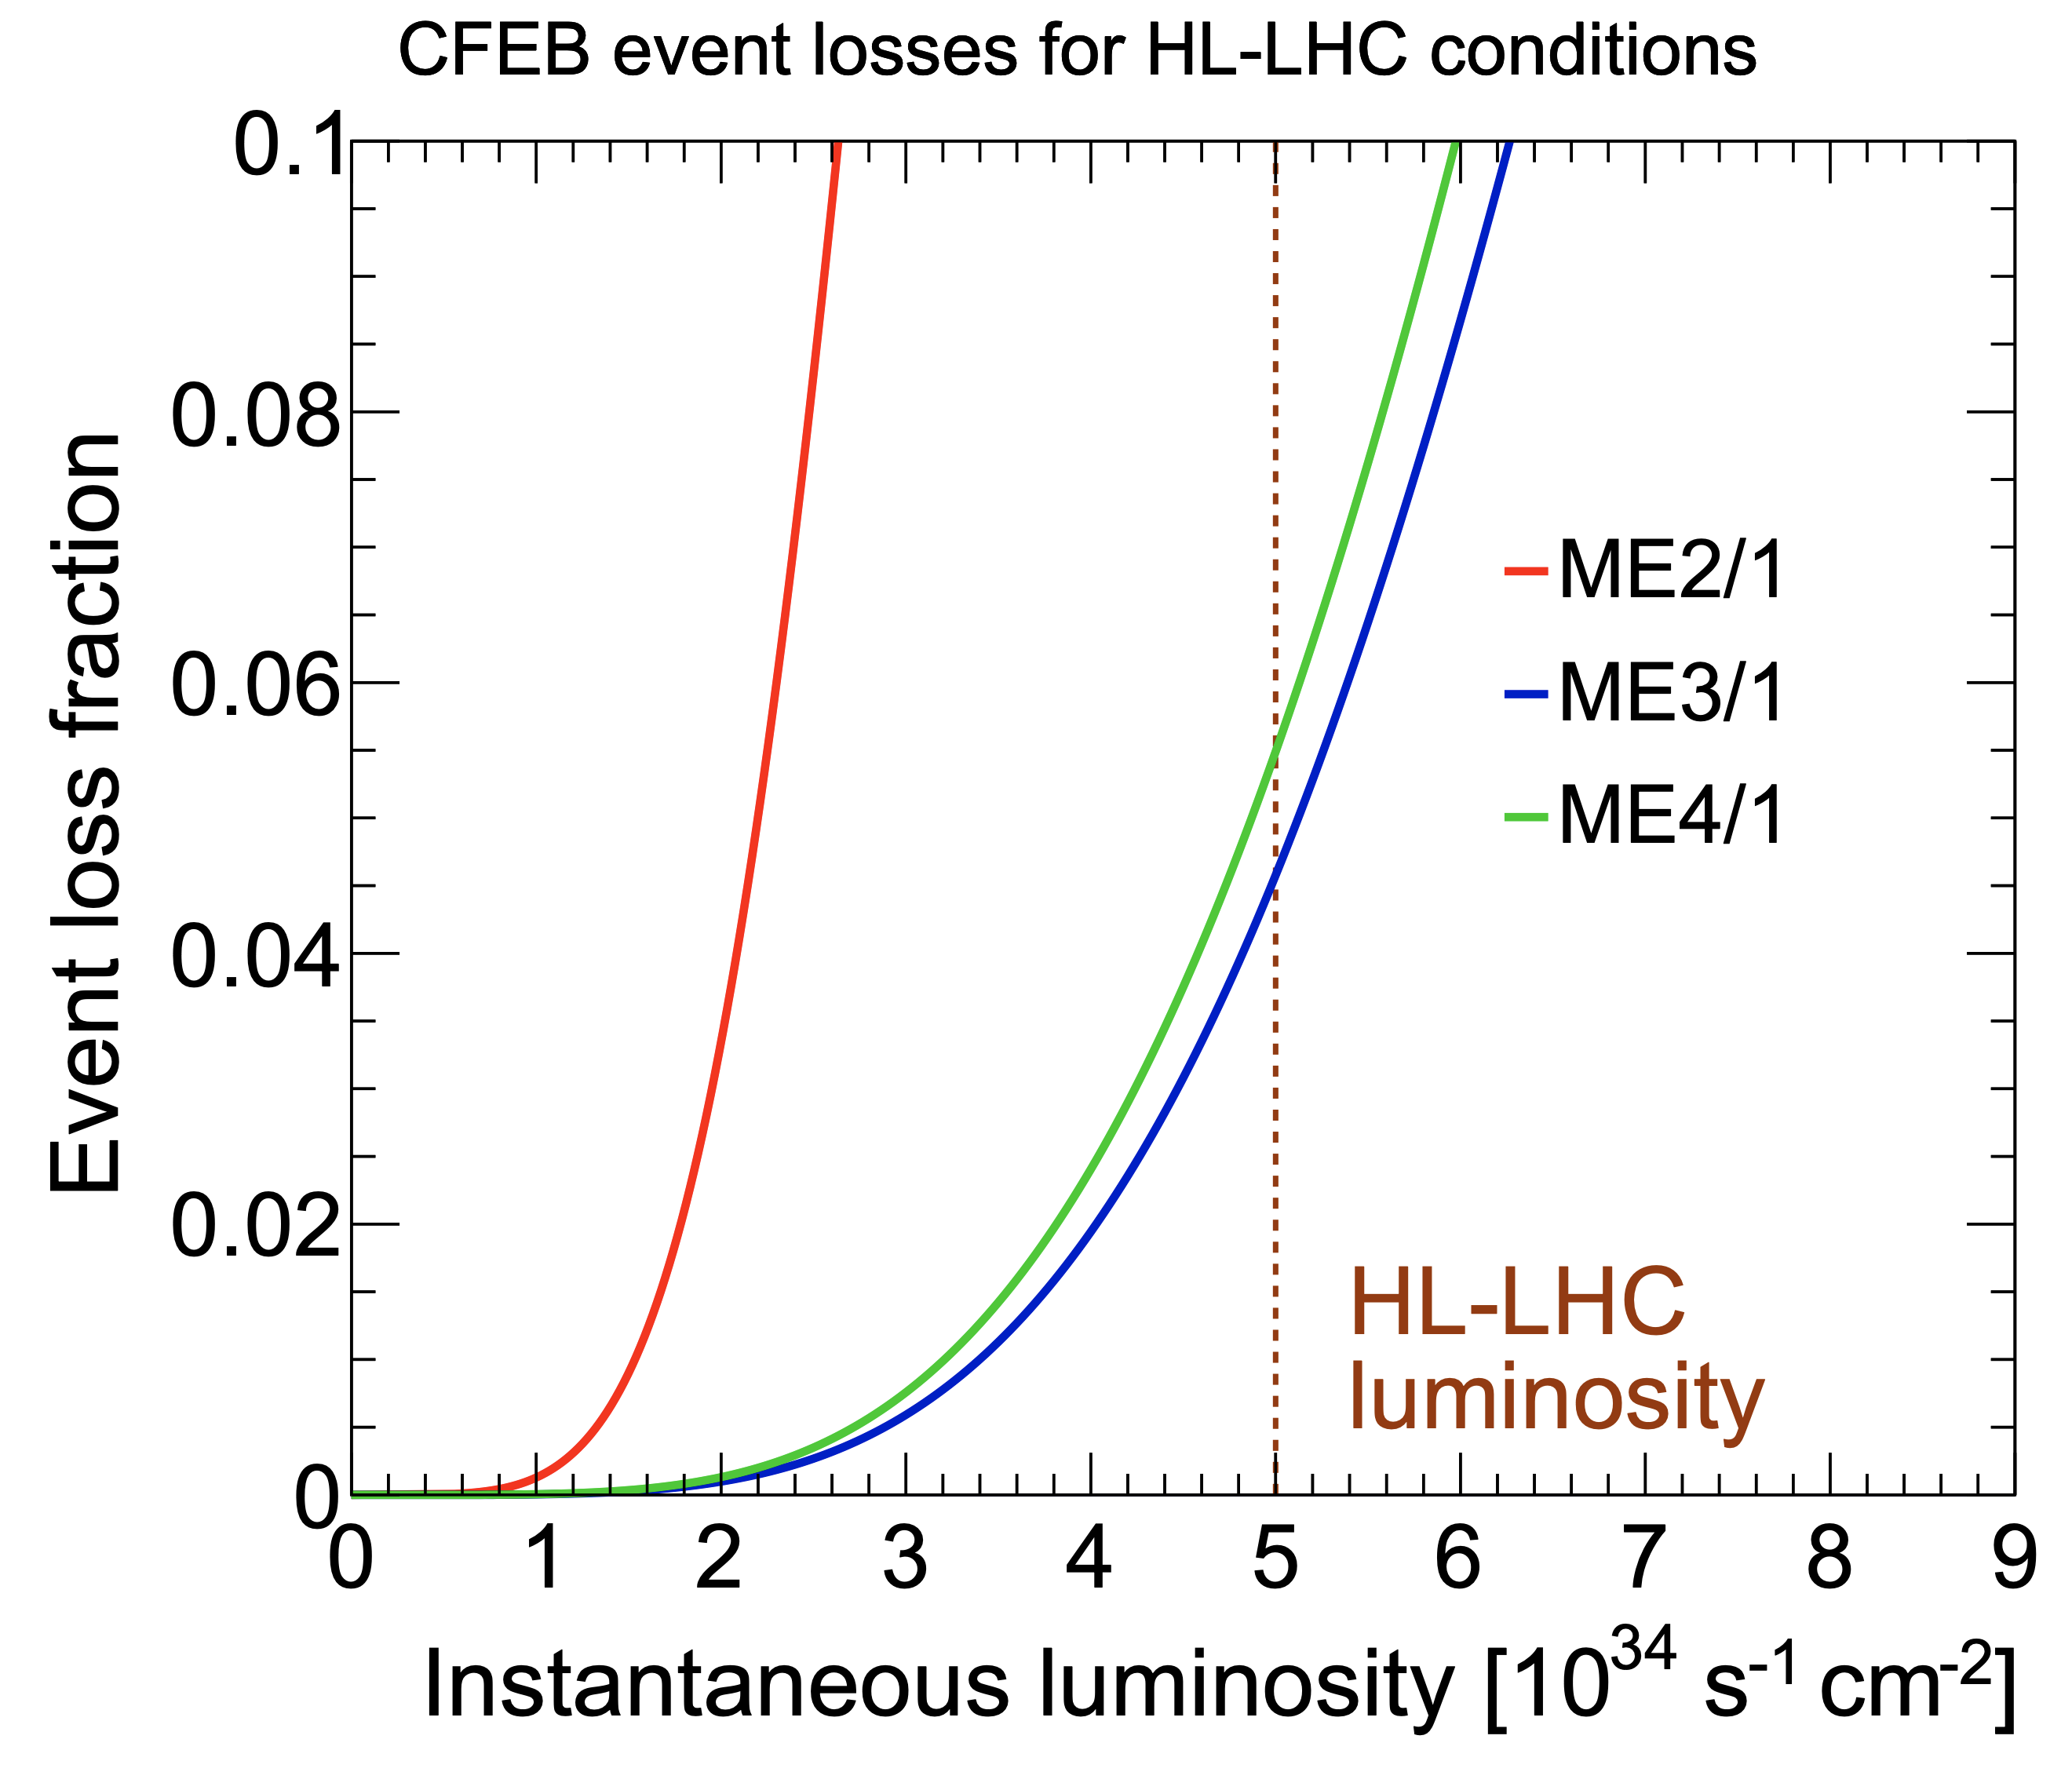
\includegraphics[width=0.49\textwidth]{Images/Phase2Upgrades/Electronics/CFEBeventlosses.png}}
    {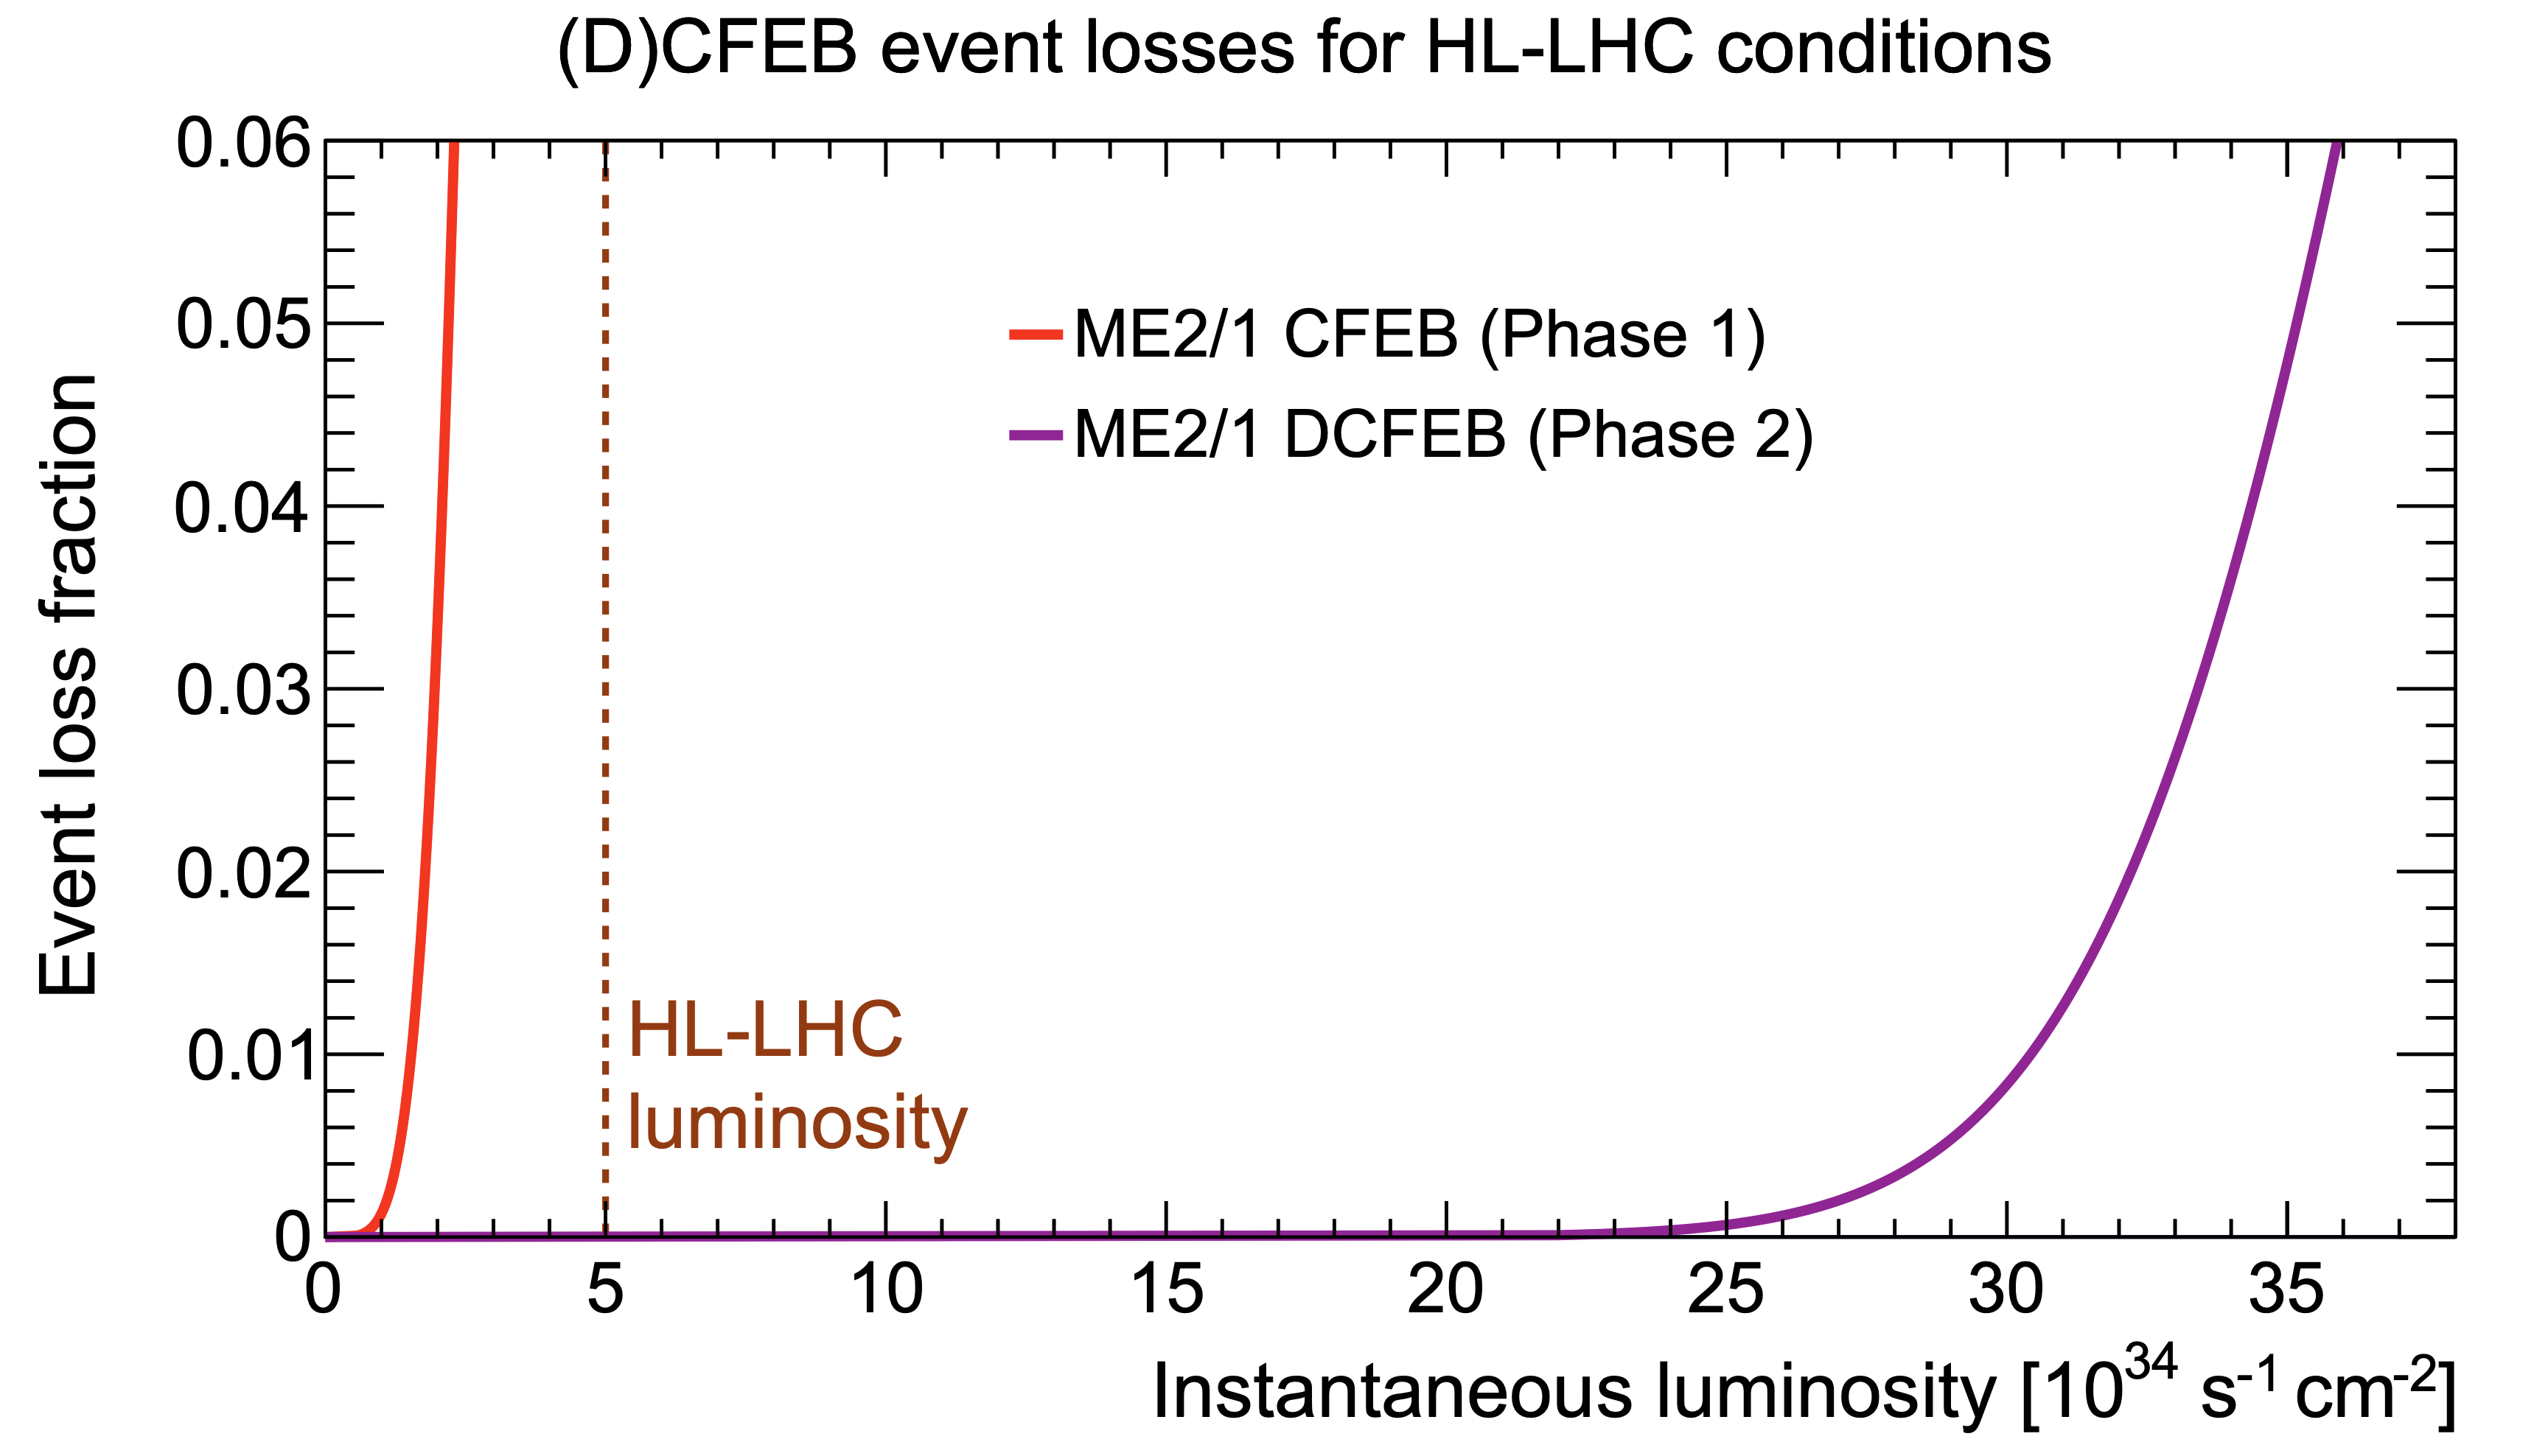
\includegraphics[width=0.49\textwidth]{Images/Phase2Upgrades/Electronics/DCFEBenetlosses.png}}
    \caption{Left: CFEB event loss fractions as a function of instantaneous luminosity on ME2/1, ME3/1, and ME4/1 chambers. Right: CFEB and DCFEB event loss fractions as a function of instantaneous luminosity on ME2/1 chambers. The plots demonstrate the need to replace the CFEBs with DCFEBs on ME234/1 chambers to avoid unacceptable data loss under HL-LHC conditions.}
    \label{fig:EventLosses}
\end{figure}

\begin{figure}[H]
    \centering
    {\includegraphics[width=1\textwidth]{Images/Phase2Upgrades/Electronics/xDCFEB.png}}
    \caption{One of seven xDCFEBs that replaced the seven DCFEBs on ME1/1 chambers in LS2.}
    \label{fig:xDCFEB}
\end{figure}

\begin{figure}[H]
    \centering
    {\includegraphics[width=1\textwidth]{Images/Phase2Upgrades/Electronics/ALCTLX150Mezz.png}}
    \caption{The ALCT-LX150 mezzanine that replaced the old ALCT mezzanines on ME1/1 chambers in LS2.}
    \label{fig:ALCT}
\end{figure}


A final set of Phase-2 upgrades will be implimented in LS3 only to off-chamber electronics. The ODMBs and DMBs of ME1/1 and ME234/1 chambers, respectively, will be replaced with ODMB7s and ODMB5s, critically increasing the output bandwidth from \SI{1.6}{Gb/s} to \SI{10}{Gb/s}. The ODMB5s will also provide optical links to the DCFEBs, replacing the legacy copper DAQ channels still in use on ME234/1 chambers throughout Run 3. An upgrade to the backend system to handle the output DAQ rates of the ODMB7 and ODMB5, featuring new FED boards for all MEx/1 chambers, will also be installed during LS3. A schematic of ME1/1 and ME234/1 CSC electronics prior to and following the Phase 2 upgrades is shown in Fig.~\ref{fig:CSCdiagram}.

\begin{figure}[H]
    \centering
    {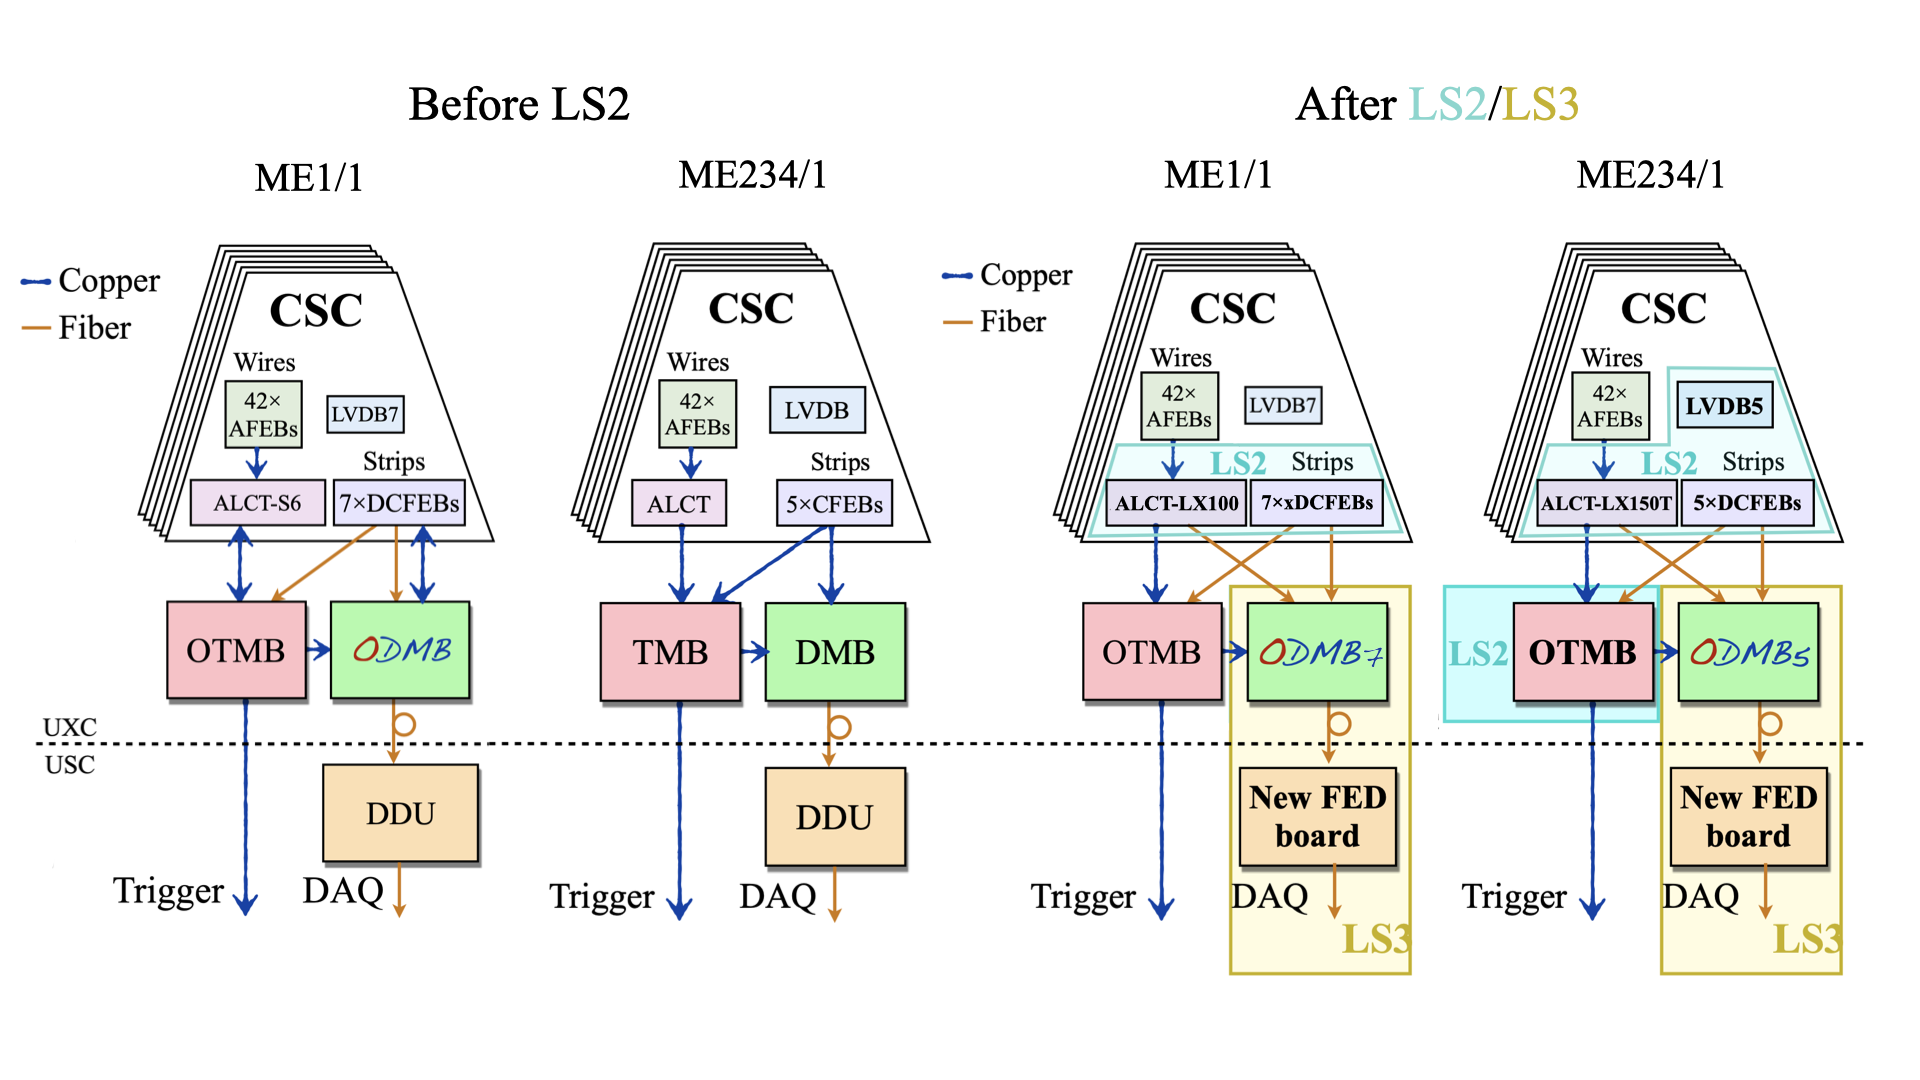
\includegraphics[width=1\textwidth]{Images/Phase2Upgrades/Electronics/CSCLS2Upgrades.png}}
    \caption{Left: Diagrams showing CSC electronics prior to LS2 on ME1/1 (far-left) and ME234/1 (second-from-left) chambers. Right: Diagrams showing CSC electronics after LS3 on ME1/1 (second-from-right) and ME234/1 (far-right) chambers. Upgrades installed during LS2 are highlighted in blue, while upgrades planned for LS3 are highlited in gold.}
    \label{fig:CSCdiagram}
\end{figure}

\section{CSC activity during LS2} \label{sec:CSCActivityDuringLS2}


Phase-2 upgrades of CMS subsytems including the replacement of the tracker, barrel ECAL and DT front-end electronics, and forward calorimeters, will be given priority during LS3. These projects require prolonged access to the CMS inner barrel and YE1 disks, so throughout LS3, CMS will remain in a configuration with both endcaps open away from the barrel. This will prevent access to the YE2 and YE3 disks on which CSCs in stations 1, 2, and 3 are mounted. Therefore, Phase-2 upgrades of the CSCs requiring the removal of chambers in those stations was scheduled for LS2, when the YE disks could be spaced apart. Upgrades of on-chamber CSC electronics would be given preference during LS2, while replacement of boards off-chamber in the peripheral crates will wait to be upgraded until LS3. Other upgrades during LS2 included Phase-1 upgrades to the HCAL and the installation of new Phase-2 GEM detectors. The full schedule of LS2 activity for CSCs upgrades followed a highly-optimized timetable of parallel chamber extraction, refurbishment, testing, installation, and commisioning of all 180 MEx/1 chambers, to be completed in just 60 weeks. The timetable was divided into four staggered workstreams based on chamber type: 1. ME+1/1, 2. ME+234/1, 3. ME-1/1, and 4. ME-234/1. Excellent progress at approximately two chambers per day was sustained throughout 2019 with workstreams 1-3, however, the outbreak of the Covid-19 pandemic presented significant setbacks to workflow and manpower, causing delays toward the end of LS2. In response, the CSC team made every effort to finish the upgrades as quickly and safely as possible, and despite a two-and-a-half month shift and a two month extension of the 4th work stream, by 2021 all CSC upgrade activity had succesfully concluded in time for Run 3 preparations.

\subsection{Chamber extraction} \label{sec:ChamberExtraction}

One at a time, chambers were disconnected from water, gas, and cabling before they were be detached from the endcap yokes. Once dismounted, CSCs were brought to the surface with an overhead crane. Inside the surface building SX5 is a CSC facility where refurbishment and testing sites are located. Extracted chambers were placed horizontally on rolling tables for in situ refurbishment and transport to each testing site within the CSC facility, while a backlog of chambers awaiting refurbishment or installation were kept vertically on storage cradles. Extraction began with the ME1/1 chambers so their DCFEBs could be harvested for the ME234/1 chambers, but parallel testing sites allowed both types to undergo refurbishment and testing simultaneously. A photograph of the CSC facility in SX5 is shown in Fig.~\ref{fig:SX5}.

\begin{figure}[H]
    \centering
    \includegraphics[width=1\textwidth]{Images/Phase2Upgrades/CSCactivity/SX5Lab.png}
    \caption{An aerial view of the CSC facility in SX5 used for the Phase-2 refurbishment and testing of CSC modules during LS1 and LS2.}
    \label{fig:SX5}
\end{figure}

\subsection{DCFEB temperature study} \label{sec:DCFEBTemperatureStudy}
The on-chamber electronics boards mounted to the face of each CSC generate a significant amount of heat while operating, a load of roughly \SI{70}{W} per chamber, and need a cooling system to prevent overheating. Beneath the (D)CFEBs, ALCTs, LVDB(5)s, and AFEBs, are copper plates, with a continuous 1/4'' copper tube brazed to each plate. Thermal pads are layered on each electronics component (ASICs, FPGAs, etc.) to provide good thermal contact with the copper plates, efficiently carrying heat away from the electronics. A photograph of a cooling cover and thermal pad strips for a DCFEB is shown in Fig.~\ref{fig:CoolingCover}. A pressurized water system flows through each chamber's copper loop and cools the plates. The supply and return ends of each chamber's copper pipe are connected via flexible hosing to neighboring CSCs forming three-chamber circuits, which are then connected to a larger cooling manifold secured to each YE disk, allowing water to flow through all the CSCs. Input water temperature is approximately 18-\SI{20}{\celsius} and is optimized to limit the temperature rise per connection to \SI{2}{\celsius}.

\begin{figure}[H]
    \centering
    \includegraphics[width=1\textwidth]{Images/Phase2Upgrades/DCFEBTempStudy/DCFEBpadding.png}
    \caption{}
    \label{fig:CoolingCover}
\end{figure}

To validate that the cooling system on ME234/1 chambers is sufficient to cool the DCFEBs that will replace the CFEBs, the efficiency of the thermal-pad-to-cooling-plate configuration was studied. An ME3/1 chamber refurbished with DCFEBs was connected to cooling and LV power using one of the FAST sites in the CSC lab at SX5 (see Sec.~\ref{sec:ChamberTesting}). With the power supply on and the DCFEBs left idle, the temperature of each DCFEBs' FPGA (using a built-in thermometer) was collected via a web-based monitor (the so-called ``yellow page'') on a minute-by-minute basis in half-hour sessions. The cooling efficiency of several configurations were studied by varying the thermal pad thickness, DCFEB location on-chamber, and type of copper cooling cover. 

It was observed that that FPGAs exibit a large temperature variation, roughly a \SI{10}{\celsius} range between DCFEBs. By swapping the location of two of the five DCFEBs on the chamber, which are arranged side-by-side, it was established that the temperature variations were an artifact of each DCFEB and that the cooling system provides a homogenous temperature map accross the DCFEBs, shown in Figs.~\ref{fig:FPGAtemp1}-\ref{fig:FPGAtemp2}. The rise in temperature of FPGA 466 in the right-hand plot of Fig.~\ref{fig:FPGAtemp1} was due to poor thermal contact with the cooling cover. DCFEBs (and CFEBs) are not actually mounted to the cooling baseplate, rather, they are secured to copper cooling covers, offset with \SI{5.0}{mm} stand-offs, and the cover is screwed to the baseplate. It is the cover that the FPGAs (and most other electronics) are in thermal contact with, while strips of thermal padding between the cover and the baseplate carry heat from the cover to the cooling system. By removing the threading in the holes of the cover it can be screwed down closer to the baseplate, providing better thermal contact, and reducing the overall temperature of the FPGAs (see Fig.~\ref{fig:FPGAtemp2}). A later study revealed that \SI{1.5}{mm}-thick thermal pads provided better thermal contact over \SI{1.0}{mm}-thick thermal pads.

\begin{figure}[H]
    \centering
    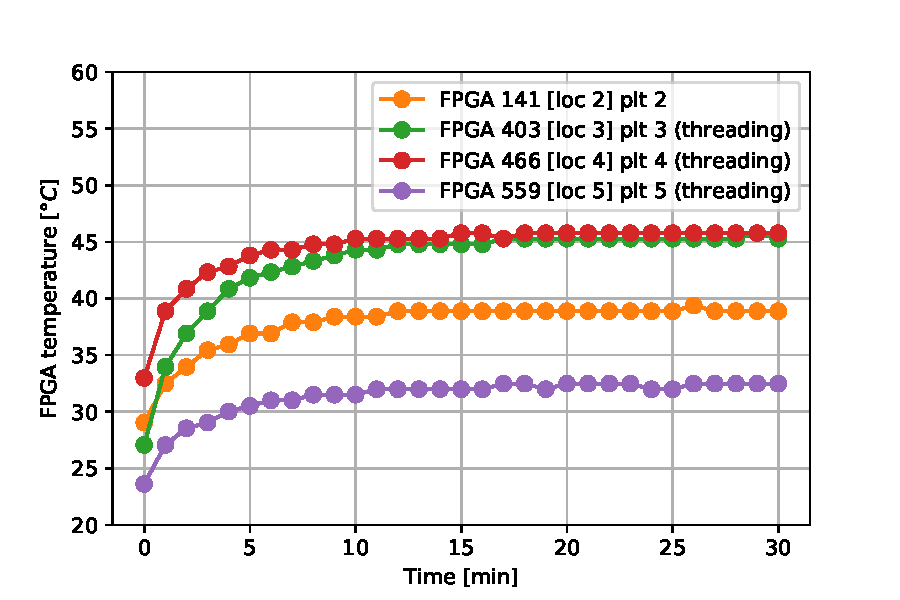
\includegraphics[width=0.49\textwidth]{Images/Phase2Upgrades/DCFEBTempStudy/TempPlot_2019_01_14_plot1-5295.pdf}
    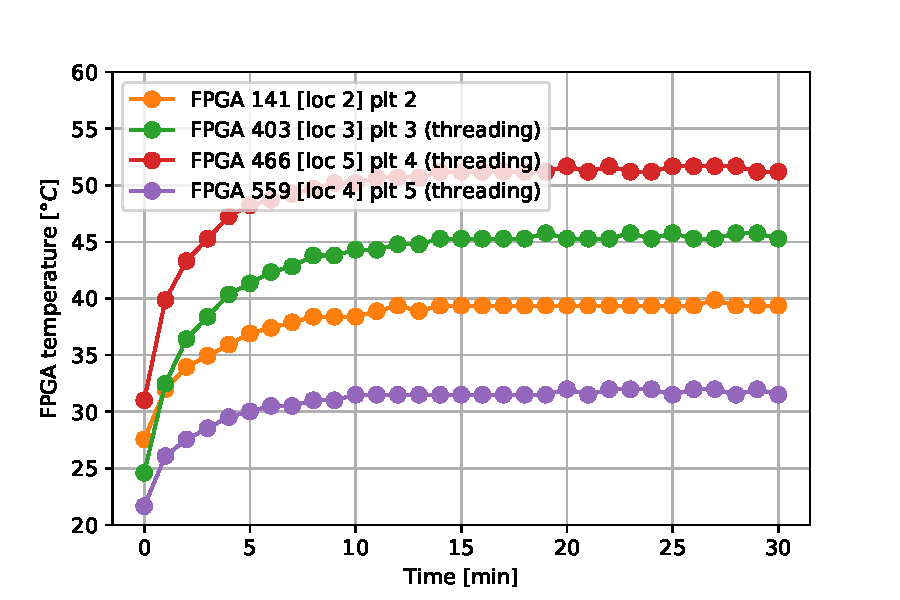
\includegraphics[width=0.49\textwidth]{Images/Phase2Upgrades/DCFEBTempStudy/TempPlot_2019_01_14_plot2-5296.pdf}
    \caption{FPGA temperature sampled every minute of five idle DCFEBs on an ME3/1 CSC. The location on-chamber of DCFEBs 466 and 559 have been swapped betweeen the two plots. The cooling plates on DCFEBs 403, 466, and 559 have threading.}
    \label{fig:FPGAtemp1}
\end{figure}

\begin{figure}[H]
    \centering
    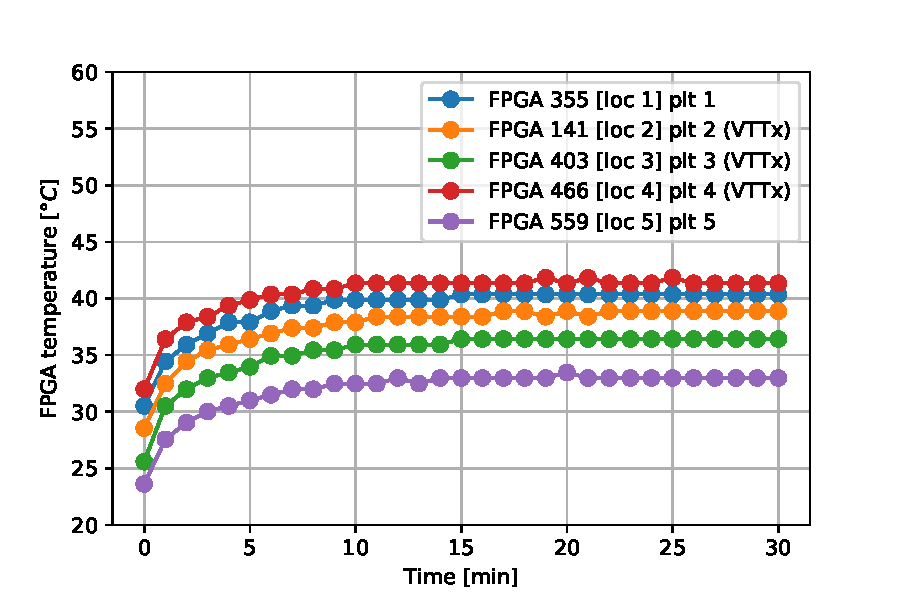
\includegraphics[width=0.49\textwidth]{Images/Phase2Upgrades/DCFEBTempStudy/TempPlot_2019_01_17_nothread12345-5433.pdf}
    \includegraphics[width=0.49\textwidth]{Images/Phase2Upgrades/DCFEBTempStudy/TempPlot_2019_01_17_nothread12354-5430.pdf}
    \caption{FPGA temperature sampled every minute of five idle DCFEBs on an ME3/1 CSC. The location on-chamber of DCFEBs 466 and 559 have been swapped betweeen the two plots. The cooling plates on all DCFEBs have no threading.}
    \label{fig:FPGAtemp2}
\end{figure}

\subsection{ME1/1 refurbishment} \label{sec:ME1/1refurbishment}

Refurbishment of each chamber was performed by a dedicated team: roughly 20 CSC group members comprised of post-docs, graduate students, and some undergraduate students, all of whom received training in the assembly and disassembly for both ME1/1 and ME234/1 chambers, as the construction and placement of the on-chamber electronics are somewhat different between the two chamber types. Chambers were refurbished at the CSC lab in SX5, following a detailed checklist. The refurbishment procedure of the ME1/1 chambers during LS2 was modeled after the ME1/1 upgrade program from LS1. A rough outline of the steps required to upgrade each electronic component is: 

\begin{itemize}
    \item LVDB7:
    \begin{enumerate}
        \item LVDB7 cover is removed and inspected for any damage
        \item LVDB7 cover is reattached (no LVDB upgrades on ME1/1)
    \end{enumerate}
    \item xDCFEBs:
    \begin{enumerate}
        \item DCFEB covers are removed, and strip cables, LV cables, and patch cables (connecting CFEBs together) are all disconnected
        \item Starting from the top of the chamber, and working down, all seven DCFEBs are unscrewed, removed, serialized and dated, and taken to temporary storage following radiation-safe guidelines
        \item Clean xDCFEBs covers with ethanol, cut and place thermal pads onto covers
        \item New xDCFEBs are installed, screwed down, and reconnected to strip, LV, and patch cables
        \item DCFEB covers are reattached
    \end{enumerate}
    \item ALCT-LX100:
    \begin{enumerate}
        \item ALCT-S6 cover is removed and all cables disconnected
        \item ALCT-S6 mezzanine is removed
        \item Thermal block with thermal pad placed on baseboard
        \item New ALCT-LX100 inserted gently to connector and secured
    \end{enumerate}
\end{itemize}

\subsection{ME234/1 refurbishment} \label{sec:ME234/1refurbishment}

As each ME1/1 chamber was refurbished, the DCFEBs harvested from that chamber were taken off-site to have their VTTx adapter boards installed. After the DCFEBs returned to the CSC lab in SX5, refurbishment of the ME234/1 chambers was carried out by the refurbishment team in situ, following a checklist similar to that used for ME1/1 chambers. The procedure is as follows: 

\begin{itemize}
    \item LVDB5:
    \begin{enumerate}
        \item LVDB cover, LVMB mezzanine, and thermal pads are removed
        \item LVDB baseboard is unscrewed and barcodes are applied to LVDB baseboard and LVMB mezzanine
        \item New thermal padding is cut and applied to LVDB5 baseboard
        \item New LVDB5 baseboard is installed and screwed down
        \item LVMB mezzanine is installed
    \end{enumerate}
    \item DCFEBs:
    \begin{enumerate}
        \item CFEB cover and individual cooling plates are removed, and strip cables, LV cables, and patch cables (connecting CFEBs together) are all disconnected
        \item All five CFEBs are unscrewed, removed, serialized and dated, and taken to storage following radiation-safe guidelines
        \item DCFEBs harvested from ME1/1 chambers are installed, screwed down, and reconnected to strip, LV, and patch cables
        \item DCFEB cooling plates and covers are reattached
    \end{enumerate}
    \item ALCT-LX150T:
    \begin{enumerate}
        \item ALCT mezzanine is removed
        \item Thermal block with thermal pad placed on baseboard
        \item New ALCT-LX150T inserted gently to connector and secured
    \end{enumerate}
    \item Optical fibers:
    \begin{enumerate}
        \item LC connectors on the optical fiber fan-out are connected to each DCFEB and ALCT, while the MTP connector is secured to the side of the chamber (more info on the optical fibers in Sec.~\ref{sec:OpticalFibers})
    \end{enumerate}
\end{itemize}

\subsection{Chamber testing} \label{sec:ChamberTesting}

Once a CSC has been refurbished but prior to reinstallation, it undergoes a series of tests designed to load firmware, validate the performance of the newly installed electronics, and identify any mistakes made during refurbishement. Chamber testing prior to reinstallation is a three-stage process: initial testing at the Final Assembly and System Testing (FAST) site, long-term testing at the Long-Term Testing (LTT) site, and final testing again at the FAST site. Both FAST and LTT sites are located inside the CSC lab at SX5 and consist of parallel testing stands (FAST 1 and FAST 2; LTT 1, LTT 2, and a third ME1/1-dedicated LTT stand) that allow 2-3 chambers to efficiently undergo testing simultaniously. A photograph of the author inspecting a CSC at the FAST testing sites in SX5 is shown in Fig.~\ref{fig:FAST}.

\begin{figure}[H]
    \centering
    \includegraphics[width=1\textwidth]{Images/Phase2Upgrades/CSCactivity/FASTsites.png}
    \caption{FAST test stands at the CSC facility in SX5. An ME1/1 chamber undergoing testing is connected to one FAST site (left-hand-side of photo), while the author inspects an ME2/1 chamber connected to the other FAST site (middle of photo).}
    \label{fig:FAST}
\end{figure}

The FAST sites are equipped to supply each CSC with high and low voltage, gas, cooling, and trigger and data links to a dedicated peripheral crate. After connecting the chamber to power, high voltage supply, trigger/DAQ readout cables to OTMB and ODMB, and both gas and water supplies, the (x)DCFEB and ALCT mezzanine firmware is uploaded and the trigger timing is synchronized. Next, a comprehensive assessment of the health of a CSC's on-chamber electronics is conducted with a suite of tests called the System Test of Endcap Peripheral crates and chamber electronics (STEP) . The STEP tests follow the sequence:
\begin{itemize}
    \item AFEB threshold and analog noise
    \item AFEB connectivity and crosstalk
    \item AFEB counting noise
    \item ALCT-AFEB time delay
    \item CFEB pedestals
    \item CFEB connectivity
    \item CFEB pulse shape and crosstalk
    \item CFEB gain
    \item Comparator thresholds and analog noise
    \item Comparator logic
    \item ALCT trigger
    \item High-statistics cosmics
\end{itemize}

Typically, all the FAST testing, including the STEP tests, takes about six hours to perform for two chambers in parallel. However, when problems with the electronics are revealed, it can take up to a day of debugging until the chamber again passes all testing at the FAST site. Common issues revealed from FAST tests include connection issues (usually fixed with reseating cables), problematic electronic boards (requires examination, repair, or replacement by experts), and chamber problems like shorted strips, broke, wires, etc., which are noted but left alone.

After finishing the STEP tests, chambers are brought to the neighboring LTT sites for 48-hour monitoring. The LTT stands supply the chambers with low voltage, gas, and cooling---no high voltage is needed. Voltage, current, and temperature stability are all monitored for a minimum of 48 hours, finishing with the low voltage portion of the STEP tests. Finally, two hours of post-LTT tests back at the FAST sites reveal if there are any gas leaks.

\subsection{Chamber installation and commissioning} \label{sec:CSCInstallationAndCommissioning}

Immediately following refurbishment and testing, each CSC was lowered back down into the experimental cavern (UXC) to be reinstalled on CMS. Chambers are reinstalled onto the YE disks in nearly the same way they are extracted, however, prior to connecting gas, water, and HV---with only LV to power the electronics---the chambers undergo initial testing of connectivity and mapping. Next, the on-board clocks of the electronics for each CSC must be configured with respect to each other to account for differences in location and cable length. After reconnecting all services, the chambers are commissioned by recording cosmic rays. Following succesfull commissioning, the upgraded CSCs are integrated with the rest of CMS and the global DAQ system, where the chambers can participate in global data taking. Hit occupancy and timing plots allow the overall functioning of the CSCs to be monitored.



\section{Optical fibers} \label{sec:OpticalFibers}

The Phase-2 transition of ME234/1 chambers from CFEBs to DCFEBs with optical links, and from DMBs to ODMBs for the corresponding chambers, requires replacing the copper connections with optical fibers for fast trigger and data readout. Throughout LS2, the muon endcaps were opened to access to the CSCs so the ME234/1 chambers could be extracted, refurbished with DCFEBs above ground, brought back down into the experimental cavern, and reinstalled. In LS3 however, acces to the CSCs will not be possible as other subsystems will have priorety access to complete Phase-2 upgrades to their detectors. However, access to the peripheral crates is possible during LS3 and that is when the ODMBs will be installed. However, this constraint meant that the optical fibers had to be installed in LS2, dispite not seeing use until LHC Run 4 after the ODMBs are in place.

Each ME234/1 chamber has five DCFEBs, each with an optical trigger and data readout, and an ALCT with data readout. In Phase-2, these readouts will be mapped to an OTMB and ODMB, with housed in a peripheral crate with OTMBs and ODMBs for three nearby chambers. ME234/1 chambers are connected to a peripheral crate with a single Sylex 48-fiber bundle trunk per peripheral crate. The chamber side of each trunk splits into four 12-fiber bundles (labeled 1-4) with MTP connections that map to eight 5- or 7- fiber bundles (labeled A-H), also with MTP connections. Specifications and for the trunk from Sylex are provided in Fig.~\ref{fig:trunkspecs}, along with a table of the channel mapping. Three of the chamber-side fiber bundles are connected to a chamber, while the fourth fiber bundle is kept as a spare. Each fiber bundle is connected to the five DCFEBs of a CSC via a 12-fiber optical ``fanout,'' with an MTP connection to the fiber bundle and LC connections to the DCFEBs. Channel mapping is as follows: one fiber for the trigger VTTx connection and the DAQ VTRx connection on each of the five DCFEBs ($2\times 5$), and two fibers for the ALCT with a trigger VTTx connection, totalling twelve channels. Figure~\ref{fig:fanouttrunkcartoon} shows a cartoon of how the 12-fiber fanout and 48-fiber bundle trunk will connect from chamber to peripheral crate.

\begin{figure}[H]
    \centering
    {\includegraphics[width=1\textwidth]{Images/Phase2Upgrades/OpticalFibers/TRUNK_C2202.pdf}}
    \caption{A technical diagram and manufacturer's specifications for a 48-fiber bundle trunk.}
    \label{fig:trunkspecs}
\end{figure}

\begin{figure}[H]
    \centering
    {\includegraphics[width=1\textwidth]{Images/Phase2Upgrades/OpticalFibers/FanoutTrunkCartoon.png}}
    \caption{A cartoon diagram depicting the fanout-to-trunk setup for three CSCs, from chamber to peripheral crate.}
    \label{fig:fanouttrunkcartoon}
\end{figure}

Functionality and mapping of the 48-fiber bundle trunks were tested in building 904 at the CERN Prevessin site. The testing setup consisted of an ME1/1 chamber, who's DCFEB acted as a constant light source. The LC ends of a 12-fiber fanout were connected to the DCFEB and the MTP end was connected to fiber bundles 1-4. The other end of the trunk, bundles A-H, were also connected to the MTP end of a second fiber fanout, and the LC connectors of those were connected to an attenuation meter. By observing light in all 48 fibers channel, one by one, the mapping of each fiber on the four-bundle-split to the eight-bindle-split of the trunk was validated. Optical attenuation measurements were consistent accross channels and within the manufacturer's specifications, shown in Fig.. At the CSC facility in SX5, mapping and attenuation of ten 12-fiber fanouts were studied, using a setup similar to the one used in bulding 904, the difference being the 48 fiber bundle trunk was replaced with a single 12-fiber bundle trunk with just one MTP connection on each end. A photograph of the SX5 setup is provided in Fig.~\ref{fig:fibertestsetup}. Optical attenuation measurements made for each of the ten 12-fiber fanouts can be found in Fig.~\ref{fig:fanoutattenuation}.

\begin{figure}[H]
    \centering
    {\includegraphics[width=0.49\textwidth]{Images/Phase2Upgrades/OpticalFibers/FanoutTesting.png}}
    \caption{The 12-fiber fanout testing setup at the CSC facility in SX5. The LC-ends of a fanout were connected to the Finnesar links on right-most DCFEB (obscured by a cooling cover). On the table in the foreground is one of the 12-fiber fanouts being tested, connnected to the the 12-fiber trunk and the optical attenuation meter.}
    \label{fig:fibertestsetup}
\end{figure}

\begin{figure}[H]
    \centering
    {\includegraphics[width=0.75\textwidth]{Images/Phase2Upgrades/OpticalFibers/FanoutAttenuation.png}}
    \caption{Optical attenuation in each channel of ten 12-fiber fanouts. Each color corresponds to a different fanout.}
    \label{fig:fanoutattenuation}
\end{figure}

Routing of the thirty-six 48-fiber bundle trunks was performed during LS2 when access to CSC stations 1, 2, and 3 was possible. As the orientation of chambers in stations alternate in each endcap, two routing configurations were used, shown in Fig.~\ref{fig:fiberrouting}. Fiber bundle trunks were secured to the sides of ME234/2 chambers with sticky pads and cable ties (the procedure is demonstrated in the two photographs of Fig.~\ref{fig:MishaGabrielRoutingFibers}), while the MTP ends on the rack-side of the trunk were bound together and wrapped in a platic bag. During LS3, the fiber bundles will be connected to each chamber and to the OTMB and ODMB in the peripheral racks. Prior to routing, labels were applied to all the trunks: two on the middle trunk near the two splits, and one near the MTP connector on each bundle. Chamber-side bundles were labeled with either the chamber (e.g., ``ME-1/1/1'') or ``SPARE,'' while crate-side bundles were labeled with the rack/crate/slot numbers, chamber, and either TRG or DAQ, depending on if the bundle was for trigger or data channels. The middle of the trunks were labeled with the chamber range/TRG+DAQ/rack/crate and a barcode.

\begin{figure}[H]
    \centering
    {\includegraphics[width=0.49\textwidth]{Images/Phase2Upgrades/OpticalFibers/FiberRouting1.png}}
    {\includegraphics[width=0.49\textwidth]{Images/Phase2Upgrades/OpticalFibers/FiberRouting2.png}}
    \caption{A schematic of the 48-fiber bundle trunk routing configurations on different endcap disks. Left: Fiber routing for clockwise-oriented stations, ME+2, ME-3, and ME-4. Right: Fiber routing for counter-clockwise-oriented stations, ME-2, ME+3, and ME+4. Chambers where the fiber bundle/trunk is connected/secured to the HV side are labeled in red, while chambers where the fiber bundle/trunk is connected/secured to the non-HV side are labeled in red.}
    \label{fig:fiberrouting}
\end{figure}

\begin{figure}[H]
    \centering
    {\includegraphics[width=0.49\textwidth]{Images/Phase2Upgrades/OpticalFibers/MishaRoutingFibers.jpeg}}
    {\includegraphics[width=0.49\textwidth]{Images/Phase2Upgrades/OpticalFibers/GabrielRoutingFibers.png}}
    \caption{Routing of the 48-fiber bundle trunks on the ME+2 disk by Misha Ignatenko (left) and the author (right).}
    \label{fig:MishaGabrielRoutingFibers}
\end{figure}

\chapter{Detector Performance} \label{chapter:DetectorPerformance}
\section{CSC conditions data} \label{sec:CSCConditionsData}



\subsection{Alignment}

 Sources of misalignment within the muon spectrometer include: chamber construction tolerances, e.g., wire-positioning; detector assembly, opening, and closing tolerances, and static deformations in the YE disks from magnetic field distortions can all result in individual chamber displacement of up to several cm from their nominal positions; and dynamic sub-millimeter misalignment from temperature fluctuations during operation. To capitalize on the \SI{100}{\micro m}-level rechit resolution in the muon system, knowledge of each sensor and module position must be aquired to an even greater precision. The Muon Alignment (MA) system continuously monitors the detector geometry with LEDs and laser beams, along with distance and angle measuring devices. All 250 DTs are continuosuly monitored, while only 12 select CSCs are monitored in each ME station are directly monitored.


\subsection{Electronics calibration}\label{sec:CSCcalib}

CSC front-end electronics require calibration to homogenize the signals in each cathode channel for HLT and offline reconstruction. Periodic tests are performed by the CSC Operations Group to configure parameters for each electronics module and extract the data needed to calibrate, usually at the start of LHC runs or after major changes to the CSCs have been made. Each CFEB on a CSC reads 96 cathode strip channels distributed accross six 16-channel amplifier-shaper ASIC chips. The shaper-amplifiers are sampled every \SI{50}{ns} and voltages are stored by the same number of 16-channel SCAs while waiting for an L1A (latency of 120 bunch crossings). The amplifier-shaper chips come equipped with internal capacitors for generating test pulses. Calibration runs inject these test pulses into all cathode channels, and by measuring the corresponding output, the constants needed to calibrate each channel can be extracted, specifically:
\begin{itemize}
    \item Strip channel electronic gains
    \item Strip pedestals
    \item Strip channel noise
    \item Strip-to-strip crosstalk
\end{itemize}
Calibrating these parameters can improve the accuracy of hit positions in recorded data reconstruction and allow for more truthful modeling of the CSCs in simulation.

\subsubsection{Gains}
Electronic gain in each strip channel is measured by incrementing the test pulse amplitude and sampling the output. During reconstruction of muon hit positions, the raw pulse heights in each channel are normalized to the average pulse-height gain accross all channels in all CSCs.

\subsubsection{Pedestals}
Pedestal values for each strip are gathered by sampling the amplifier output at \SI{20}{MHz} without any input signal and measuring the charge in each SCA bin, referred to as ``static'' pedestals. Static pedestals are used in simulation to supply a baseline for simulated signals. High-rates during normal operation can result in a baseline shift. To account for this, reconstruction instead uses ``dynamic'' pedestals, where the average charge on each strip of only the first two SCA time bins---prior to the signal arrival---are taken as the pedestal values. 

\subsubsection{Noise matrix}
As the pedestal noise (RMS) is correlated accross SCA time bins, it can be described for each strip by the covarience between the charge in each SCA time bin, forming a symmetric ``noise matrix.'' Each element of the noise matrix is defined as 
\begin{equation}
C_{ij} = \langle Q_i \cdot Q_j \rangle - \langle Q_i \rangle \cdot \langle Q_j \rangle,
\end{equation}
where $Q_i$ is the charge in SCA time bin $i$, and the average is taken over many calibration runs.

\subsubsection{Crosstalk}
Undesirable signal transfer called crosstalk can occur between neighboring strips in a CSC through inductive coupling. To measure the effect, an approximate delta-function pulse is fired into each amplifier channel. The induced charge on an adjacent strip normalized to the charge deposited on a strip are measured in each SCA time bin. This charge ratio is then convoluted with the expected ion drift time and electron arrival time distributions to model the amplifier response to a pulse shape typically seen during CSC operation (instead of a delta-function pulse). The  crosstalk fraction for each channel, per SCA time bin, is defined as the ratio of the left or right neighboring strips divided by the sum of all three adjacent strips. Crosstalk fractions ordinarily range from 5~\% to 10~\%. As the crosstalk fraction is linear in time (within \SI{160}{ns} of the charge peak), it can be encoded for each channel into just four constants: the slope and intercept of a straight line representing the crosstalk coupling to the left and right neighbors of a strip as a function of SCA time bin. For every strip and SCA time bin, these conditions are stored as a $3\times3$ matrix whose elements transform the measured charges on a strip and its two neighbors to the input charge on the strip. The matrices are used in simulated data to model crosstalk, while the inverse matrices can be applied in recorded data to remove the effect of crosstalk.

\subsection{Offline timing corrections}

In addition to supplying the muon system with precise muon track postions and directions, the CSCs assist the RPCs in determining the arrival time of muons in the endcaps. As mentioned in Sec.~\ref{sec:CSCcalib}, the CFEB amplifier channels are only sampled every \SI{50}{ns}, where the first two of the eight SCA time bins are used to measure the dynamic pedestal. To obtain a precise measurement of the arrival time of a signal peak, the signal shape is compared to the known analytical form of the pulse shaped by the CFEB amplifier-shaper ASICs. The resulting rechit time resolution in each CSC is measured to be \SI{5}{ns}. The average cathode rechit times in each chamber are shifted to zero using ``heuristic'' corrections that are data-derived using muons from collisions. Anode clocks are more coarse-grain than the cathode timing, defined by identifying the closest cathode time bin with a \SI{12.5}{ns} resolution, modulo a roughly \SI{205}{ns} offset. Cathode hit times and anode hit times are combined to arrive at CSC segment times. A Gaussian fit to the segment time distribution in each chamber provides a segment timing resolution of roughly \SI{3}{ns}.

\subsection{Dead channels and chambers}

During operation, it is possible for CSC strip and wire channels to die, and in more extreme cases, entire chambers. These can sometimes be recovered, but often the chamber is inaccessible, preventing any hands-on intervention to revive it. Dead chambers are identified when CSC data quality monitoring does not see rechits in the chamber. A catalogue of dead channels and chambers for a given period of running are classified as CSC conditions data. While not needed for processing real data, these conditions data are important to accurately model the state of the real CSCs in simulation. In practice, the CSC group only used a list of ``bad'' chambers, represented in simulation by not generating rechits in the channels of those chambers.

\subsection{Mapping, geometry, and gas gain}

Other CSC conditions data are stored in the conditions database but are never updated. Electronics cable mapping (for crates, chambers, and DDUs) are used in real data as hardware labels to geometric values. CSC strip and wire geometry information is used in simulation for digitization and in real data during local reconstruction. Chamber parameters traditionally associated with strip and wire geometry are likewise used in simulation and real data. Precise corrections to the system gas gain were derived in a detailed analysis during Run I.
  

\section{CSC Validation} \label{sec:CSCValidation}
\input{Text/Chapters/DetectorPerformance/Sections/CSCValidation}

\chapter{Search for pair-produced leptoquarks decaying to bottom quarks and muons} \label{chapter:LeptoquarkSearch}
\section{Introduction} \label{sec:Introduction}
% Introduce HEP and collider physics, SM




The ultimate aim of particle physics is to build a complete theoretical model consistent with all observed natural phenomena at the smallest size-scales. Experiments over the past century have revealed that matter is composite in nature, formed from irreducible constituants called elementary particles. Particles are also responsible for three of the four fundamental forces in the universe. The mathematical framework to describe the catalog of observed particles was developed is called the Standard Model (SM) of particle physics. The SM has been hugely succesful in describing the properties and behavior of elementary particles, and made accurate predictions for new particles that were subsequently discovered. The massive particles composing matter are six leptons: the electrically charged electron, muon, and tau, and their neutral counterparts, neutrinos; and six quarks: up, down, top, bottom, charm, and strange. The force carrying particles are the gauge bosons: a massless photon responsible for electromagnetism (or light), the charged \PW and neutral \PZ bosons responsible for the weak nuclear force (causing neutron decay) and eight massless gluons responsible for the strong nuclear force (this binds quarks together to form hadrons, e.g., protons and neutrons, and similarly binds protons and neutrons together inside atomic nuclei). The remaining particle in the SM is the Higgs boson, which through a phenomena called the Higgs mechanism is responsible for providing masses to all the SM particles.
 
Most elementary particles at rest are not stable; heavier particles rapidly decay into lighter particles like electrons found in atomic orbitals, up or down quarks that form stable nuclei, or the photons we observe as light or radiation. To study the more massive, unstable elementary particles rarely found in nature, particle physicists produce them by generating a sufficient quantity of energy. High Energy Physics (HEP) experiments accomplish this feat by accelerating particles---either along a ring or a linear tunnel---until they are brought into contact in spectacular head-on collisions. In rare instances, a heavy particle is created from the energy of the collision before decaying back into lighter constituants. Extremely sensitive detectors surrounding the collision points record the particles that emerge from the collisions. By studying the species of particles that emerge from each collision and their kinematics, the properties of the original heavy particle can be deduced.

Many particle accelerators have been built that vary in the particles they collide and the center-of-mass collision energies they can generate. The current highest energy collisions belong to the Large Hadron Collider (LHC) at CERN in Geneva Switzerland. The LHC is a \SI{27}{\km} ring that delivers nearly a billion proton-proton collisions per second to a number of experiments along its circumference, reaching collision energies of \SI{13}{\TeV}. The CMS experiment is one of two general purpose detectors at the LHC that has succesfully tested a wide range of SM phenomena with astonishing precision, and most noteably codiscovered the Higgs boson with the ATLAS experiment in 2012.

% Gaps in the SM and possible solution
Although the SM has continued to hold up against the most stringent experiemental tests, the theory still suffers from a number of shortcomings, such as: the remarkable symmetry between the lepton and quark generations lacks any explaination; the electromagnetic and weak forces unite at high energy scales into a single electroweak force (verified at the LHC), but the strong force remains separate at all energy scales; and the measured hierarchy of the electroweak force and gravity---spanning 24 orders of magnitude---requires excessive fine-tuning to model. Supersymmetry (SUSY), Grand Unified Theories (GUTs), composite models with lepton and quark substructure, and Technicolor schemes are several extensions to the SM put forward to explain these some of these limitations. Predicted in these theories are new heavy bosons that would couple to both a lepton and quark. Such leptoquarks (an obvious portmanteau) are color-triplet spin 0 or spin 1 bosons, carrying both baryon and lepton quantum numbers, and fractional electric charge. The values of these parameters classify each leptoquark model, while other parameters including the mass \MLQ, coupling strength at a leptoquark-lepton-quark vertex \lambdaLQ, and decay branching fraction into charged leptons \bfu are model independent. Leptoquarks remain excellent candidates to test theories of new physics, as they can be readily produced in hadron colliders.

Searches by the CDF and \DZERO collaborations at Fermilab's Tevetron collider in the 1990's and 2000's looked for pair-produced leptoquarks constrained to decays into quarks and leptons of the same generation. Proton-antiproton collision energies at the Tevetron reaching \SI{1.96}{\TeV} allowed the experiments to place lower bounds on the masses of first-, second-, and third-generation scalar leptoquarks, assuming decays into two charged leptons or one charged lepton and one neutrino.

Overlapping with this time period, the H1 and ZEUS collaborations at the DESY HERA collider searched for both single- and pair-produced leptoquarks in \SI{300}{\GeV} electron-proton collisions. Searches similarly looked for leptoquarks by fermion generation, but also included searches that allowed mixing of quark-lepton generations. In 1997, the H1 and ZEUS collaborations reported a data excess corresponding to a  first-generation leptoquark with a mass of roughly \SI{200}{\GeV}, known as the HERA anomaly. This was ultimately ruled out with the accumulation of more data.

% Current limits
With data collected during Run I of the LHC, the CMS and ATLAS collaborations brought the hunt for leptoquarks into a new energy regime with 7 and \SI{8}{\TeV} proton-proton collisions. The wide-ranging scope of both collaborations' leptoquark search programs led to numerous publications placeing exclusion limits on single- and pair-production leptoquarks in a host of search channels. Run II of the LHC increased collision energies to \SI{13}{\TeV}, opening up sensitivity to higher kinematic regimes. In October 2022, the ATLAS experiment published results in a single paper covering searches for pair-produced scalar and vector leptoquarks decaying into third generation quarks (\Ptop and \Pbottom) and first or second generation leptons (\Pe, \Pmu, and \Pnu). The extensive analysis placed lower bounds on leptoquark masses in eight final state channels. The most rigorous experimental limits to date on scalar leptoquarks decaying into muons have been set by the CMS collaboration. Using \SI{35.9}{\invfb} of data recorded by the CMS detector in 2016, leptoquarks in the \mumujj channel with masses below \SI{1530}{\GeV} were excluded with a \SI{95}{\%} \CL. Interest in leptoquarks has grown in recent years; flavor anomalies observed by the LHCb collaboration and measurements of the muon anomaly in tension with the SM by the Muon~$g-2$ collaboration both hint at new physics for which leptoquarks (especially second-generation) remain ideal contenders to explain.

% Proposed search
Presented is a thesis detailing a novel search for pair-produced scalar leptoquarks decaying to a pair of muons and two jets, with at least one jet identified as orginating from a bottom quark. Proton-proton collision data at \SI{13}{\TeV} collected with the CMS detector in 2016, 2017, and 2018 are used, corresponding to an integrated luminosity of \SI{138}{\invfb}. Leptoquark searches requiring two muons are well motivated as they leave a clean signature in the detector. While past leptoquark searches by the CMS collaboration have confined couplings to leptons and quarks of the same generation, the inclusion of a b-tag requirement in association with muons targets leptoquark models that allow intergenerational mixing, motivated by the flavor anomalies. This represents the first analysis of CMS data targeting leptoquarks decaying to muons and b quarks, and the first leptoquark search with a muon in the final state to make use of the entire Run II dataset recorded by the CMS detector. 30 mass hypotheses will be tested from 300 to \SI{4000}{\GeV}, guided by limits from previous searches. The analysis will place expected and observed upper limits on leptoquark pair-production cross sections for each mass hypothesis, and by comparing results to the theoretical cross sections, these limits can be tranlated into an experimental lower bound on the leptoquark mass.

% Chapters overview 

Following the introduction, this thesis opens with a primer on the SM of particle physics in Chapter~\ref{chapter:Theory}: how elementary particles interact via fundamental forces and how spontanious breaking of symmetry in the equations governing their kinematics provides them with the masses we observe. This is followed by a description of leptoquark models and the experimental motivation for this thesis. Chapter~\ref{chapter:Experiment} covers the design of the the LHC and an overview of each CMS subdetector. The program of upgrades to the CMS muon detectors in which I participated, lasting from 2018 to 2022, is recounted in Chapter~\ref{chapter:Phase2Upgrades}. The performance of the CMS muon detectors is studied in Chapter~\ref{chapter:DetectorPerformance}, including: data processing, reconstruction of muon objects from detector information, and the alignment and calibration of the CMS muon detectors. Activity I performed during my Ph.D. studies related to the calibration of the CMS muon system concludes the detector-focused chapters. Chapter~\ref{chapter:LeptoquarkSearch} contains the analysis I carried out with CMS collision data in search of leptoquarks, including: the recorded and simulated datasets analyzed, the event selection, the data-to-simulation corrections, the estimation of SM background processes, the machine learning techniques used to separate signal-like events from background-like events, the sources of systematic uncertainty accounted for, and the results of the search. Closing remarks summarizing the results of the leptoquark search and exploring possible future studies are provided in Chapter~\ref{chapter:Conclusion}.  

\section{Samples} \label{sec:Samples}
\subsection{Data samples} \label{sec:Data}

\subsection{Simulated signal samples} \label{sec:SimSignal}

\subsection{Simulated background samples} \label{sec:SimBackground}

\section{Corrections} \label{sec:Corrections}
\subsection{Muon momentum scale} \label{sec:MES}

\subsection{Muon momentum resolution} \label{sec:MER}

\subsection{Muon ID and isolation efficiency} \label{sec:MuonIDIsoEff}

\subsection{Muon reconstruction efficiency} \label{sec:MuonRecoEff}

\subsection{Trigger efficiency} \label{sec:MuonHLTEff}

\subsection{Jet corrections} \label{sec:JEC}

\subsection{MET corrections} \label{sec:METCorr}

\subsection{b-Jet identification} \label{sec:BJetID}

\subsection{HEM 15/16 failure} \label{sec:HEM1516Failure}

\subsection{Top \texorpdfstring{$p_T$}{pT} reweighting} \label{sec:TopPtReweighting}



\section{Event selection} \label{sec:EventSelection}
\subsection{Muon reconstruction and identification} \label{sec:MuonRecoID}

\subsection{Jet reconstruction and identification} \label{sec:JetRecoID}

\subsection{MET Reconstruction} \label{sec:METReco}

\subsection{Preselection} \label{sec:Preselection}

\subsection{b-Jet tagging} \label{sec:BJetTagging}

\section{Background estimation} \label{sec:Backgrounds}
\subsection{Estimation of \texorpdfstring{$Z/\gamma*$}{Z/y*}+jets and \texorpdfstring{$t\overline{t}$}{tt-bar} backgrounds} \label{sec:ZTTbkg}

\subsection{Data comparison} \label{sec:DataComparison}


\section{Final selection} \label{sec:FinalSelection}

After preselection, a final selection is required to optimize signal-to-background efficiency. A boosted decision tree (BDT) is trained and tested on signal and background MC, with one BDT per signal hypothesis, and a final cut is applied to each BDT discriminator. 

Training samples are constructed by randomly selecting events from the combined 2016, 2017, and 2018 MC datasets detailed in Section~\ref{sec:Samples}. The same background normalization scale factors, data and MC corrections, b-jet requirement, and preselection described in Sections~\ref{sec:EventSelection} and~\ref{sec:Corrections} are applied to the corresponding year's MC. Additional cuts of $\Muu > \SI{250}{\GeV}$ and $\Muujj > \MLQ$ are applied, to reduce training bias in background-enriched and low-signal regions. After training, a separate sample is constructed from the same MC and in the same way, and tested on each BDT to verify there is no overfitting (there is no overlap in training and testing events). A set of 11 kinematic variables---identified for their strong signal-to-background separation power---are used as input variables to the BDTs: 
\begin{itemize}
    \item Invariant masses: \Muu, \Muujj, \MujOne, \MujTwo
    \item Final state object momenta: \ptof{\PmuOne}, \ptof{\PmuTwo}, \ptof{\PjOne}, \ptof{\PjTwo}
    \item Combined momenta: \ST, \MET
    \item Spatial separation between the combined (vectorially-summed) momenta of the dimuon pair and the leading-\pt jet: \DRof{\PmuOne+\PmuTwo}{\PjOne}
\end{itemize}
Further details, including a number of studies, can be found in Appendix~\ref{app:BDTPerformance}.

To extract the highest possible signal, a cut on the BDT response is optimized using the Punzi significance~\cite{Punzi} as a figure of merit, defined here:

\begin{equation}
    \frac{\epsilon(t)}{a/2+\sqrt{B(t)}}
    \label{eq:punzi}
\end{equation}

where $\epsilon(t)$ is the signal efficiency for a cut $t$, $a$ is the chosen sigma significance ($a = 5$ in this analysis), and $B(t)$ is the number of background events after applying a cut $t$.

A comparison between observed and expected data at preselection in the BDT score at every leptoquark mass point is shown in Figures~\ref{figapp:BDT300to1400}--\ref{figapp:BDT2700to4000}. Final selection cuts are optimized and applied to the BDT score for each leptoquark mass, while the same cut value is used accross all years. A cut log is listed in Table~\ref{tab:cutlog}. To ensure all events at final selection are contained within the signal region (SR) and do not overlap with events in the background normalization CRs (where the SR and CRs are defined in Table~\ref{tab:srcrdefs}), an additional cut of $\Muu > \SI{250}{\GeV}$ is applied. Additionally, the same \MLQ-dependent cut used in the BDT training is applied at final selection: $\Muujj > \MLQ$. Efficiency in signal and background from applying each final selection cut is shown in Fig.~\ref{figapp:efficiency} for all three years of data-taking. Efficiency here is defined as the number of events passing the final selection (optimized BDT score, $\Muu > \SI{250}{\GeV}$, and $\Muujj > \MLQ$ cuts) divided by the number of events present at preselection (in both the numerator and denominator, the b-jet tag requirement, normalization scale factors, and MC corrections are applied). Event yields at final selection are provided for each year of data taking in Tables~\ref{tab:eventyields2016}--\ref{tab:eventyields2018}. W+Jets has been ommited from the tables as no events pass the final selection---it is kept in the analysis for the background normalization estimation, BDT training, systematic uncertainty estimation, etc. Figures~\ref{figapp:finalSelMuu}--\ref{figapp:finalSelDRuuj1} show the BDT input variables at final selection in 2016, 2017, and 2018 signal and background simulation for several representative leptoquark mass points. Plots showing the Punzi significance as a function of the BDT score, for each BDT, are shown in Figs.~\ref{figapp:punzivsbdt1}--\ref{figapp:punzivsbdt2}.

\begin{table}[H]
    \caption{The \ZJETS (A), \ttbar (B), and $\VV + \TTV$ (C) background normalization CR, and SR definitions.}
    \begin{center}
           %\scriptsize
           \begin{tabular}{cccc}\hline\hline
                Region      & Mass window [\GeV]                 & Additional selection \\ \hline
                Control A   & $80 < \Muu < 100$     & $N_{\jets} = 2$, $N_{\jets} = 3$, $N_{\jets} = 4$, or $N_{\jets} \geq 5$ \\ 
                Control B   & $100 < \Muu < 250$    & - \\ 
                Control C   & $80 < \Muu < 100$     & $N_{\text{leptons}}\geq 3$, $N_{\text{b-jets}}\geq 0$ \\
                Signal      & $250 < \Muu$          & - \\ \hline\hline
           \end{tabular}
           \label{tab:srcrdefs}
    \end{center}
\end{table}


%%%%%%%%%%%%%%%%%%%%%%%%%%%%%%%%%%%%%%%%%%%%%%%%%%%%%%%%%%%%%%%%%%%%%%%%%%%%%%%%%%%%%%%%%%
%%%%%%%%%%%%%%%%%%%%%%%%%%%%%%%%%%%%%%%%%% 2016 %%%%%%%%%%%%%%%%%%%%%%%%%%%%%%%%%%%%%%%%%%
%%%%%%%%%%%%%%%%%%%%%%%%%%%%%%%%%%%%%%%%%%%%%%%%%%%%%%%%%%%%%%%%%%%%%%%%%%%%%%%%%%%%%%%%%%




% 2016 final sel + pt20 veto

\begin{table}[H]
	\tiny
	\begin{center}
		\caption{Event yields in 2016 data at the final selection level. Uncertainties are statistical unless otherwise indicated.}
		\begin{tabular}{ccccccccc}
			\hline \hline
            \MLQ  &     Signal &              	 \ZJETS &                       \ttbar &                    \TTV &           	    \VV &                       Single Top &            All BG (stat + syst)&                               Data \\ \hline	
            300  &      18810 $\pm$ 240  &    	 0.686 $\pm$ 0.089  &           0.13 $\pm$ 0.13  &          0.0423 $\pm$ 0.0061  &  0.242 $\pm$ 0.059  &        0.0 $\pm$ 0.0  &        1.1 $\pm$ 0.16  $\pm$ 0.11  &                       0 \\
            400  &      5501 $\pm$ 59  &      	 0.79 $\pm$ 0.11  &             0.0 $ _{-0.0}^{+0.13}$   &  0.012 $\pm$ 0.003  &    0.0 $ _{-0.0}^{+0.014}$   & 0.378 $\pm$ 0.267  &    1.18 $ _{-0.29}^{+0.32}$   $\pm$ 0.13  &            0 \\
            500  &      3405 $\pm$ 24  &      	 0.719 $\pm$ 0.078  &           0.586 $\pm$ 0.338  &        0.025 $\pm$ 0.005  &    0.0537 $\pm$ 0.019  &       0.407 $\pm$ 0.288  &    1.79 $\pm$ 0.45  $\pm$ 0.12  &                      2 \\
            600  &      1379.9 $\pm$ 8.9  &   	 0.218 $\pm$ 0.031  &           0.0 $ _{-0.0}^{+0.13}$   &  0.018 $\pm$ 0.005  &    0.0462 $\pm$ 0.0207  &      0.0 $\pm$ 0.0  &        0.282 $ _{-0.037}^{+0.131}$   $\pm$ 0.037  &        0 \\
            700  &      706.9 $\pm$ 4.0  &    	 0.283 $\pm$ 0.035  &           0.0 $ _{-0.0}^{+0.13}$   &  0.021 $\pm$ 0.004  &    0.0 $ _{-0.0}^{+0.014}$   & 0.0 $\pm$ 0.0  &        0.304 $ _{-0.035}^{+0.132}$   $\pm$ 0.053  &        0 \\
            800  &      333.1 $\pm$ 1.7  &    	 0.0 $ _{-0.0}^{+0.011}$   &    0.0 $ _{-0.0}^{+0.13}$   &  0.0057 $\pm$ 0.0015  &  0.0063 $\pm$ 0.0032  &      0.0 $\pm$ 0.0  &        0.012 $ _{-0.003}^{+0.127}$   $\pm$ 0.001  &        0 \\
            900  &      165.48 $\pm$ 0.81  &  	 0.103 $\pm$ 0.013  &           0.0 $ _{-0.0}^{+0.13}$   &  0.011 $\pm$ 0.004  &    0.065 $\pm$ 0.026  &        0.0 $\pm$ 0.0  &        0.179 $ _{-0.03}^{+0.129}$   $\pm$ 0.018  &         0 \\
            1000  &     83.44 $\pm$ 0.46  &   	 0.15 $\pm$ 0.018  &            0.0 $ _{-0.0}^{+0.13}$   &  0.01 $\pm$ 0.004  &     0.058 $\pm$ 0.026  &        0.0 $\pm$ 0.0  &        0.219 $ _{-0.032}^{+0.13}$   $\pm$ 0.024  &         1 \\
            1100  &     45.57 $\pm$ 0.2  &    	 0.4 $\pm$ 0.047  &             0.0 $ _{-0.0}^{+0.13}$   &  0.0181 $\pm$ 0.0064  &  0.0415 $\pm$ 0.0207  &      0.0 $\pm$ 0.0  &        0.46 $ _{-0.052}^{+0.136}$   $\pm$ 0.086  &         1 \\
            1200  &     21.345 $\pm$ 0.098  & 	 0.086 $\pm$ 0.016  &           0.0 $ _{-0.0}^{+0.13}$   &  0.0053 $\pm$ 0.0027  &  0.0 $ _{-0.0}^{+0.014}$   & 0.19 $\pm$ 0.19  &      0.282 $ _{-0.191}^{+0.229}$   $\pm$ 0.03  &         1 \\
            1300  &     11.244 $\pm$ 0.051  & 	 0.0466 $\pm$ 0.0113  &         0.0 $ _{-0.0}^{+0.13}$   &  0.0 $\pm$ 0.0  &        0.0 $ _{-0.0}^{+0.014}$   & 0.0 $\pm$ 0.0  &        0.0478 $ _{-0.0113}^{+0.1274}$   $\pm$ 0.0078  &    0 \\
            1400  &     7.011 $\pm$ 0.029  &  	 0.186 $\pm$ 0.028  &           0.0 $ _{-0.0}^{+0.13}$   &  0.0 $\pm$ 0.0  &        0.0 $ _{-0.0}^{+0.014}$   & 0.19 $\pm$ 0.19  &      0.376 $ _{-0.192}^{+0.23}$   $\pm$ 0.042  &         0 \\
            1500  &     3.384 $\pm$ 0.015  &  	 0.0221 $\pm$ 0.0052  &         0.0 $ _{-0.0}^{+0.13}$   &  0.0 $\pm$ 0.0  &        0.013 $\pm$ 0.013  &        0.0 $\pm$ 0.0  &        0.037 $ _{-0.014}^{+0.127}$   $\pm$ 0.005  &        0 \\
            1600  &     1.9368 $\pm$ 0.0081  &	 0.174 $\pm$ 0.038  &           0.0 $ _{-0.0}^{+0.13}$   &  0.0 $\pm$ 0.0  &        0.0 $ _{-0.0}^{+0.014}$   & 0.0 $\pm$ 0.0  &        0.174 $ _{-0.038}^{+0.132}$   $\pm$ 0.032  &        0 \\
            1700  &     1.0235 $\pm$ 0.0052  &	 0.0306 $\pm$ 0.0092  &         0.0 $ _{-0.0}^{+0.13}$   &  0.0 $\pm$ 0.0  &        0.0 $ _{-0.0}^{+0.014}$   & 0.0 $\pm$ 0.0  &        0.0306 $ _{-0.0092}^{+0.1272}$   $\pm$ 0.0058  &    0 \\
            1800  &     0.56 $\pm$ 0.0  &     	 0.0 $\pm$ 0.0  &               0.0 $ _{-0.0}^{+0.13}$   &  0.0 $\pm$ 0.0  &        0.0 $ _{-0.0}^{+0.014}$   & 0.0 $\pm$ 0.0  &        0.0 $ _{-0.0}^{+0.13}$   $\pm$ 0.0  &               0 \\
            1900  &     0.33 $\pm$ 0.0  &     	 0.088 $\pm$ 0.018  &           0.0 $ _{-0.0}^{+0.13}$   &  0.0 $\pm$ 0.0  &        0.0 $ _{-0.0}^{+0.014}$   & 0.0 $\pm$ 0.0  &        0.088 $ _{-0.018}^{+0.128}$   $\pm$ 0.02  &         0 \\
            2000  &     0.185 $\pm$ 0.001  &  	 0.062 $\pm$ 0.019  &           0.0 $ _{-0.0}^{+0.13}$   &  0.0 $\pm$ 0.0  &        0.013 $\pm$ 0.013  &        0.0 $\pm$ 0.0  &        0.075 $ _{-0.024}^{+0.128}$   $\pm$ 0.017  &        0 \\
            2100  &     0.102 $\pm$ 0.0  &    	 0.072 $\pm$ 0.02  &            0.0 $ _{-0.0}^{+0.13}$   &  0.0 $\pm$ 0.0  &        0.0 $ _{-0.0}^{+0.014}$   & 0.0 $\pm$ 0.0  &        0.072 $ _{-0.02}^{+0.128}$   $\pm$ 0.027  &         0 \\
            2200  &     0.053 $\pm$ 0.0  &    	 0.0291 $\pm$ 0.0168  &         0.0 $ _{-0.0}^{+0.13}$   &  0.0 $\pm$ 0.0  &        0.0 $ _{-0.0}^{+0.014}$   & 0.0 $\pm$ 0.0  &        0.0291 $ _{-0.0168}^{+0.128}$   $\pm$ 0.0084  &     0 \\
            2300  &     0.03 $\pm$ 0.0  &     	 0.038 $\pm$ 0.016  &           0.0 $ _{-0.0}^{+0.13}$   &  0.0 $\pm$ 0.0  &        0.0 $ _{-0.0}^{+0.014}$   & 0.0 $\pm$ 0.0  &        0.038 $ _{-0.016}^{+0.128}$   $\pm$ 0.012  &        0 \\
            2400  &     0.017 $\pm$ 0.0  &    	 0.0149 $\pm$ 0.0056  &         0.0 $ _{-0.0}^{+0.13}$   &  0.0 $\pm$ 0.0  &        0.0 $ _{-0.0}^{+0.014}$   & 0.0 $\pm$ 0.0  &        0.0149 $ _{-0.0056}^{+0.127}$   $\pm$ 0.0061  &     0 \\
            2500  &     0.0099 $\pm$ 0.0  &   	 0.0 $\pm$ 0.0  &               0.0 $ _{-0.0}^{+0.13}$   &  0.0 $\pm$ 0.0  &        0.0 $ _{-0.0}^{+0.014}$   & 0.0 $\pm$ 0.0  &        0.0 $ _{-0.0}^{+0.13}$   $\pm$ 0.0  &               0 \\
            2600  &     0.0055 $\pm$ 0.0  &   	 0.0 $\pm$ 0.0  &               0.0 $ _{-0.0}^{+0.13}$   &  0.0 $\pm$ 0.0  &        0.0 $ _{-0.0}^{+0.014}$   & 0.0 $\pm$ 0.0  &        0.0 $ _{-0.0}^{+0.13}$   $\pm$ 0.0  &               0 \\
            2700  &     0.0 $\pm$ 0.0  &      	 0.036 $\pm$ 0.016  &           0.0 $ _{-0.0}^{+0.13}$   &  0.0 $\pm$ 0.0  &        0.0 $ _{-0.0}^{+0.014}$   & 0.0 $\pm$ 0.0  &        0.036 $ _{-0.016}^{+0.128}$   $\pm$ 0.018  &        0 \\
            2800  &     0.0 $\pm$ 0.0  &      	 0.0 $ _{-0.0}^{+0.011}$   &    0.0 $ _{-0.0}^{+0.13}$   &  0.0 $\pm$ 0.0  &        0.0 $ _{-0.0}^{+0.014}$   & 0.0 $\pm$ 0.0  &        0.0 $ _{-0.0}^{+0.13}$   $\pm$ 0.0  &               0 \\
            2900  &     0.0 $\pm$ 0.0  &      	 0.0 $ _{-0.0}^{+0.011}$   &    0.0 $ _{-0.0}^{+0.13}$   &  0.0 $\pm$ 0.0  &        0.0 $ _{-0.0}^{+0.014}$   & 0.0 $\pm$ 0.0  &        0.0 $ _{-0.0}^{+0.13}$   $\pm$ 0.0  &               0 \\
            3000  &     0.0 $\pm$ 0.0  &      	 0.0 $\pm$ 0.0  &               0.0 $ _{-0.0}^{+0.13}$   &  0.0 $\pm$ 0.0  &        0.0 $ _{-0.0}^{+0.014}$   & 0.0 $\pm$ 0.0  &        0.0 $ _{-0.0}^{+0.13}$   $\pm$ 0.0  &               0 \\
            3500  &     0.0 $\pm$ 0.0  &      	 0.028 $\pm$ 0.016  &           0.0 $ _{-0.0}^{+0.13}$   &  0.0 $\pm$ 0.0  &        0.0 $ _{-0.0}^{+0.014}$   & 0.0 $\pm$ 0.0  &        0.028 $ _{-0.016}^{+0.128}$   $\pm$ 0.034  &        0 \\
            4000  &     0.0 $\pm$ 0.0  &      	 0.0 $\pm$ 0.0  &               0.0 $ _{-0.0}^{+0.13}$   &  0.0 $\pm$ 0.0  &        0.0 $ _{-0.0}^{+0.014}$   & 0.0 $\pm$ 0.0  &        0.0 $ _{-0.0}^{+0.13}$   $\pm$ 0.0  &               0 \\
            \hline \hline
        \end{tabular}
        \label{tab:eventyields2016}
    \end{center}
\end{table}





% 2017 final sel + pt20 veto

\begin{table}[H]
	\tiny
	\begin{center}
		\caption{Event yields in 2017 data at the final selection level. Uncertainties are statistical unless otherwise indicated.}
		\begin{tabular}{ccccccccc}
			\hline \hline
            \MLQ  &     Signal &              	 \ZJETS &                       \ttbar &                    \TTV &           	    \VV &                       Single Top &                All BG (stat + syst)&                               Data \\ \hline	
            300  &      20990 $\pm$ 260  &    	 1.45 $\pm$ 0.2  &              0.59 $\pm$ 0.17  &          0.026 $\pm$ 0.005  &  	 0.0 $\pm$ 0.0  &           0.241 $\pm$ 0.17  &         2.31 $\pm$ 0.31  $\pm$ 0.23  &                      5 \\
            400  &      5952 $\pm$ 64  &      	 0.0491 $\pm$ 0.0091  &         0.093 $\pm$ 0.066  &        0.0351 $\pm$ 0.0083  &	 0.014 $\pm$ 0.005  &       0.0 $ _{-0.0}^{+0.12}$   &  0.191 $ _{-0.067}^{+0.138}$   $\pm$ 0.01  &         0 \\
            500  &      3834 $\pm$ 27  &      	 1.59 $\pm$ 0.19  &             0.258 $\pm$ 0.097  &        0.0481 $\pm$ 0.0093  &	 0.097 $\pm$ 0.028  &       0.384 $\pm$ 0.271  &        2.38 $\pm$ 0.35  $\pm$ 0.26  &                      2 \\
            600  &      1547 $\pm$ 10  &      	 0.516 $\pm$ 0.077  &           0.068 $\pm$ 0.048  &        0.012 $\pm$ 0.003  &  	 0.0 $\pm$ 0.0  &           0.0 $ _{-0.0}^{+0.12}$   &  0.597 $ _{-0.091}^{+0.151}$   $\pm$ 0.085  &        1 \\
            700  &      792.8 $\pm$ 4.4  &    	 0.558 $\pm$ 0.055  &           0.055 $\pm$ 0.055  &        0.0 $\pm$ 0.0  &      	 0.0263 $\pm$ 0.0118  &     0.0 $\pm$ 0.0  &            0.644 $\pm$ 0.078  $\pm$ 0.089  &                   0 \\
            800  &      376.3 $\pm$ 1.9  &    	 0.322 $\pm$ 0.031  &           0.056 $\pm$ 0.056  &        0.0426 $\pm$ 0.0093  &	 0.065 $\pm$ 0.029  &       0.0 $ _{-0.0}^{+0.12}$   &  0.486 $ _{-0.071}^{+0.14}$   $\pm$ 0.061  &         1 \\
            900  &      186.01 $\pm$ 0.91  &  	 0.0 $ _{-0.0}^{+0.027}$   &    0.0 $ _{-0.0}^{+0.049}$  &  0.012 $\pm$ 0.004  &  	 0.0357 $\pm$ 0.0206  &     0.0 $ _{-0.0}^{+0.12}$   &  0.0477 $ _{-0.021}^{+0.1345}$   $\pm$ 0.0094  &     0 \\
            1000  &     94.65 $\pm$ 0.44  &   	 0.178 $\pm$ 0.018  &           0.0 $ _{-0.0}^{+0.049}$  &  0.0063 $\pm$ 0.0024  &	 0.0357 $\pm$ 0.0206  &     0.0 $ _{-0.0}^{+0.12}$   &  0.22 $ _{-0.027}^{+0.133}$   $\pm$ 0.031  &         1 \\
            1100  &     51.05 $\pm$ 0.23  &   	 0.155 $\pm$ 0.016  &           0.0 $ _{-0.0}^{+0.049}$  &  0.014 $\pm$ 0.005  &  	 0.021 $\pm$ 0.012  &       0.0 $ _{-0.0}^{+0.12}$   &  0.19 $ _{-0.02}^{+0.132}$   $\pm$ 0.027  &          0 \\
            1200  &     24.26 $\pm$ 0.15  &   	 0.0 $ _{-0.0}^{+0.027}$   &    0.0 $ _{-0.0}^{+0.049}$  &  0.011 $\pm$ 0.005  &  	 0.067 $\pm$ 0.047  &       0.0 $ _{-0.0}^{+0.12}$   &  0.077 $ _{-0.047}^{+0.141}$   $\pm$ 0.014  &        0 \\
            1300  &     12.752 $\pm$ 0.08  &  	 0.0 $ _{-0.0}^{+0.027}$   &    0.0 $ _{-0.0}^{+0.049}$  &  0.0 $\pm$ 0.0  &      	 0.0258 $\pm$ 0.0258  &     0.0 $ _{-0.0}^{+0.12}$   &  0.0285 $ _{-0.0258}^{+0.1353}$   $\pm$ 0.0059  &    1 \\
            1400  &     7.961 $\pm$ 0.032  &  	 0.0709 $\pm$ 0.0082  &         0.0 $ _{-0.0}^{+0.049}$  &  0.01 $\pm$ 0.004  &   	 0.153 $\pm$ 0.088  &       0.0 $ _{-0.0}^{+0.12}$   &  0.234 $ _{-0.089}^{+0.157}$   $\pm$ 0.035  &        1 \\
            1500  &     3.851 $\pm$ 0.016  &  	 0.062 $\pm$ 0.01  &            0.0 $ _{-0.0}^{+0.049}$  &  0.0104 $\pm$ 0.0052  &	 0.0 $\pm$ 0.0  &           0.0 $ _{-0.0}^{+0.12}$   &  0.073 $ _{-0.012}^{+0.13}$   $\pm$ 0.014  &         0 \\
            1600  &     2.2027 $\pm$ 0.0091  &	 0.0234 $\pm$ 0.0043  &         0.0 $ _{-0.0}^{+0.049}$  &  0.0068 $\pm$ 0.0039  &	 0.0259 $\pm$ 0.0183  &     0.0 $ _{-0.0}^{+0.12}$   &  0.056 $ _{-0.0192}^{+0.1314}$   $\pm$ 0.0097  &     1 \\
            1700  &     1.16 $\pm$ 0.0  &     	 0.0248 $\pm$ 0.005  &          0.0 $ _{-0.0}^{+0.049}$  &  0.0068 $\pm$ 0.0039  &	 0.0 $\pm$ 0.0  &           0.0 $ _{-0.0}^{+0.12}$   &  0.0316 $ _{-0.0063}^{+0.1301}$   $\pm$ 0.0064  &    0 \\
            1800  &     0.64 $\pm$ 0.0  &     	 0.0332 $\pm$ 0.0076  &         0.0 $ _{-0.0}^{+0.049}$  &  0.0 $\pm$ 0.0  &      	 0.0 $\pm$ 0.0  &           0.0 $ _{-0.0}^{+0.12}$   &  0.0367 $ _{-0.008}^{+0.1302}$   $\pm$ 0.0093  &     0 \\
            1900  &     0.39 $\pm$ 0.0  &     	 0.0202 $\pm$ 0.0032  &         0.0 $ _{-0.0}^{+0.049}$  &  0.0104 $\pm$ 0.0052  &	 0.0259 $\pm$ 0.0183  &     0.0 $ _{-0.0}^{+0.12}$   &  0.0565 $ _{-0.0193}^{+0.1314}$   $\pm$ 0.0087  &    0 \\
            2000  &     0.22 $\pm$ 0.0  &     	 0.0371 $\pm$ 0.0069  &         0.0 $ _{-0.0}^{+0.049}$  &  0.0104 $\pm$ 0.0052  &	 0.0 $\pm$ 0.0  &           0.0 $ _{-0.0}^{+0.12}$   &  0.0477 $ _{-0.0086}^{+0.1302}$   $\pm$ 0.0135  &    0 \\
            2100  &     0.12 $\pm$ 0.0  &     	 0.0 $\pm$ 0.0  &               0.0 $ _{-0.0}^{+0.049}$  &  0.0 $\pm$ 0.0  &      	 0.0 $\pm$ 0.0  &           0.0 $ _{-0.0}^{+0.12}$   &  0.0078 $ _{-0.0024}^{+0.13}$   $\pm$ 0.0017  &      1 \\
            2200  &     0.063 $\pm$ 0.0  &    	 0.0 $ _{-0.0}^{+0.027}$   &    0.0 $ _{-0.0}^{+0.049}$  &  0.0 $\pm$ 0.0  &      	 0.0 $\pm$ 0.0  &           0.0 $ _{-0.0}^{+0.12}$   &  0.0 $ _{-0.0}^{+0.13}$   $\pm$ 0.0  &               0 \\
            2300  &     0.036 $\pm$ 0.0  &    	 0.0 $\pm$ 0.0  &               0.0 $ _{-0.0}^{+0.049}$  &  0.0 $\pm$ 0.0  &      	 0.0 $\pm$ 0.0  &           0.0 $ _{-0.0}^{+0.12}$   &  0.007 $ _{-0.0034}^{+0.13}$   $\pm$ 0.0022  &       0 \\
            2400  &     0.021 $\pm$ 0.0  &    	 0.014 $\pm$ 0.0038  &          0.0 $ _{-0.0}^{+0.049}$  &  0.0071 $\pm$ 0.0041  &	 0.0 $\pm$ 0.0  &           0.0 $ _{-0.0}^{+0.12}$   &  0.0212 $ _{-0.0056}^{+0.1301}$   $\pm$ 0.0089  &    0 \\
            2500  &     0.012 $\pm$ 0.0  &    	 0.0178 $\pm$ 0.004  &          0.0 $ _{-0.0}^{+0.049}$  &  0.0 $\pm$ 0.0  &      	 0.0 $\pm$ 0.0  &           0.0 $ _{-0.0}^{+0.12}$   &  0.0178 $ _{-0.004}^{+0.13}$   $\pm$ 0.0077  &       1 \\
            2600  &     0.0066 $\pm$ 0.0  &   	 0.0 $ _{-0.0}^{+0.027}$   &    0.0 $ _{-0.0}^{+0.049}$  &  0.0 $\pm$ 0.0  &      	 0.0 $\pm$ 0.0  &           0.0 $ _{-0.0}^{+0.12}$   &  0.0 $ _{-0.0}^{+0.13}$   $\pm$ 0.0  &               0 \\
            2700  &     0.0 $\pm$ 0.0  &      	 0.0067 $\pm$ 0.0019  &         0.0 $ _{-0.0}^{+0.049}$  &  0.0 $\pm$ 0.0  &      	 0.0 $\pm$ 0.0  &           0.0 $ _{-0.0}^{+0.12}$   &  0.0067 $ _{-0.0019}^{+0.13}$   $\pm$ 0.0037  &      0 \\
            2800  &     0.0 $\pm$ 0.0  &      	 0.0 $\pm$ 0.0  &               0.0 $ _{-0.0}^{+0.049}$  &  0.0 $\pm$ 0.0  &      	 0.0 $\pm$ 0.0  &           0.0 $ _{-0.0}^{+0.12}$   &  0.0 $ _{-0.0}^{+0.13}$   $\pm$ 0.0  &               1 \\
            2900  &     0.0 $\pm$ 0.0  &      	 0.006 $\pm$ 0.0019  &          0.0 $ _{-0.0}^{+0.049}$  &  0.0 $\pm$ 0.0  &      	 0.0 $\pm$ 0.0  &           0.0 $ _{-0.0}^{+0.12}$   &  0.006 $ _{-0.0019}^{+0.13}$   $\pm$ 0.0033  &       1 \\
            3000  &     0.0 $\pm$ 0.0  &      	 0.0 $\pm$ 0.0  &               0.0 $ _{-0.0}^{+0.049}$  &  0.0 $\pm$ 0.0  &      	 0.0 $\pm$ 0.0  &           0.0 $ _{-0.0}^{+0.12}$   &  0.0 $ _{-0.0}^{+0.13}$   $\pm$ 0.0  &               0 \\
            3500  &     0.0 $\pm$ 0.0  &      	 0.0 $ _{-0.0}^{+0.027}$   &    0.0 $ _{-0.0}^{+0.049}$  &  0.0 $\pm$ 0.0  &      	 0.0 $\pm$ 0.0  &           0.0 $ _{-0.0}^{+0.12}$   &  0.0 $ _{-0.0}^{+0.13}$   $\pm$ 0.0  &               0 \\
            4000  &     0.0 $\pm$ 0.0  &      	 0.0 $ _{-0.0}^{+0.027}$   &    0.0 $ _{-0.0}^{+0.049}$  &  0.0 $\pm$ 0.0  &      	 0.0 $\pm$ 0.0  &           0.0 $ _{-0.0}^{+0.12}$   &  0.0 $ _{-0.0}^{+0.13}$   $\pm$ 0.0  &               1 \\
            \hline \hline
        \end{tabular}
        \label{tab:eventyields2017}
    \end{center}
\end{table}



% 2018 final sel + pt20 veto

\begin{table}[H]
	\tiny
	\begin{center}
		\caption{Event yields in 2018 data at the final selection level. Uncertainties are statistical unless otherwise indicated.}
		\begin{tabular}{ccccccccc}
			\hline \hline
            \MLQ  & 	Signal &              	 \ZJETS &                   	 \ttbar &                 	     \TTV &           	     \VV &                          Single Top &                    All BG (stat + syst)&                          	    Data \\ \hline	
            300  &      32440 $\pm$ 560  &    	 1.5 $\pm$ 0.23  &          	 0.928 $\pm$ 0.28  &        	 0.11 $\pm$ 0.016  &   	 0.393 $\pm$ 0.088  &           0.464 $\pm$ 0.328  &            3.4 $\pm$ 0.5  $\pm$ 0.25  &                        0 \\
            400  &      8860 $\pm$ 140  &     	 0.0 $\pm$ 0.0  &           	 0.1387 $\pm$ 0.0801  &     	 0.0215 $\pm$ 0.0051  &	 0.0 $ _{-0.0}^{+0.02}$   &     0.0 $ _{-0.0}^{+0.23}$   &      0.163 $ _{-0.0802}^{+0.2462}$   $\pm$ 0.006  &      1 \\
            500  &      5692 $\pm$ 57  &      	 0.0 $ _{-0.0}^{+0.037}$   &	 0.276 $\pm$ 0.123  &       	 0.108 $\pm$ 0.017  &  	 0.099 $\pm$ 0.025  &           0.334 $\pm$ 0.334  &            0.818 $ _{-0.357}^{+0.359}$   $\pm$ 0.037  &        2 \\
            600  &      2288 $\pm$ 21  &      	 0.0 $ _{-0.0}^{+0.037}$   &	 0.211 $\pm$ 0.1218  &      	 0.0662 $\pm$ 0.0121  &	 0.083 $\pm$ 0.028  &           0.0 $ _{-0.0}^{+0.23}$   &      0.36 $ _{-0.126}^{+0.266}$   $\pm$ 0.016  &         3 \\
            700  &      1169.6 $\pm$ 9.2  &   	 0.302 $\pm$ 0.038  &       	 0.22 $\pm$ 0.127  &        	 0.017 $\pm$ 0.004  &  	 0.0134 $\pm$ 0.006  &          0.0 $ _{-0.0}^{+0.23}$   &      0.553 $ _{-0.133}^{+0.267}$   $\pm$ 0.046  &        1 \\
            800  &      568.8 $\pm$ 4.1  &    	 0.127 $\pm$ 0.016  &       	 0.22 $\pm$ 0.127  &        	 0.0 $\pm$ 0.0  &      	 0.085 $\pm$ 0.028  &           0.0 $ _{-0.0}^{+0.23}$   &      0.432 $ _{-0.131}^{+0.266}$   $\pm$ 0.027  &        0 \\
            900  &      282.1 $\pm$ 1.9  &    	 0.338 $\pm$ 0.041  &       	 0.0 $ _{-0.0}^{+0.084}$   &	 0.026 $\pm$ 0.0072  & 	 0.0435 $\pm$ 0.0177  &         0.0 $ _{-0.0}^{+0.23}$   &      0.407 $ _{-0.045}^{+0.251}$   $\pm$ 0.057  &        0 \\
            1000  &    	143.72 $\pm$ 0.94  &  	 0.0 $ _{-0.0}^{+0.037}$   &	 0.0687 $\pm$ 0.0687  &     	 0.007 $\pm$ 0.0019  & 	 0.0056 $\pm$ 0.0056  &         0.0 $ _{-0.0}^{+0.23}$   &      0.0813 $ _{-0.069}^{+0.2447}$   $\pm$ 0.0074  &     0 \\
            1100  &    	78.21 $\pm$ 0.49  &   	 0.175 $\pm$ 0.023  &       	 0.0759 $\pm$ 0.0759  &     	 0.0217 $\pm$ 0.006  & 	 0.0627 $\pm$ 0.0362  &         0.0 $ _{-0.0}^{+0.23}$   &      0.335 $ _{-0.087}^{+0.248}$   $\pm$ 0.032  &        0 \\
            1200  &    	37.27 $\pm$ 0.24  &   	 0.0 $ _{-0.0}^{+0.037}$   &	 0.0 $ _{-0.0}^{+0.084}$   &	 0.0147 $\pm$ 0.0073  &	 0.0056 $\pm$ 0.0056  &         0.0 $ _{-0.0}^{+0.23}$   &      0.0203 $ _{-0.0092}^{+0.2496}$   $\pm$ 0.0021  &    0 \\
            1300  &    	19.64 $\pm$ 0.12  &   	 0.0285 $\pm$ 0.0064  &     	 0.0 $ _{-0.0}^{+0.084}$   &	 0.0 $\pm$ 0.0  &      	 0.0 $ _{-0.0}^{+0.02}$   &     0.0 $ _{-0.0}^{+0.23}$   &      0.0285 $ _{-0.0064}^{+0.2476}$   $\pm$ 0.0054  &    0 \\
            1400  &    	12.419 $\pm$ 0.071  & 	 0.176 $\pm$ 0.026  &       	 0.0 $ _{-0.0}^{+0.084}$   &	 0.0213 $\pm$ 0.0081  &	 0.025 $\pm$ 0.025  &           0.0 $ _{-0.0}^{+0.23}$   &      0.223 $ _{-0.037}^{+0.25}$   $\pm$ 0.033  &         0 \\
            1500  &    	6.054 $\pm$ 0.036  &  	 0.0 $ _{-0.0}^{+0.037}$   &	 0.0 $ _{-0.0}^{+0.084}$   &	 0.0 $\pm$ 0.0  &      	 0.018 $\pm$ 0.018  &           0.0 $ _{-0.0}^{+0.23}$   &      0.02 $ _{-0.018}^{+0.25}$   $\pm$ 0.003  &          0 \\
            1600  &    	3.486 $\pm$ 0.02  &   	 0.0 $\pm$ 0.0  &           	 0.0 $ _{-0.0}^{+0.084}$   &	 0.0 $\pm$ 0.0  &      	 0.0 $ _{-0.0}^{+0.02}$   &     0.0 $ _{-0.0}^{+0.23}$   &      0.0 $ _{-0.0}^{+0.25}$   $\pm$ 0.0  &               0 \\
            1700  &    	1.878 $\pm$ 0.011  &  	 0.0374 $\pm$ 0.0132  &     	 0.0 $ _{-0.0}^{+0.084}$   &	 0.0 $\pm$ 0.0  &      	 0.0 $ _{-0.0}^{+0.02}$   &     0.0 $ _{-0.0}^{+0.23}$   &      0.0374 $ _{-0.0132}^{+0.2479}$   $\pm$ 0.0087  &    0 \\
            1800  &    	1.0336 $\pm$ 0.0061  &	 0.0 $ _{-0.0}^{+0.037}$   &	 0.0 $ _{-0.0}^{+0.084}$   &	 0.0 $\pm$ 0.0  &      	 0.0 $ _{-0.0}^{+0.02}$   &     0.0 $ _{-0.0}^{+0.23}$   &      0.0 $ _{-0.0}^{+0.25}$   $\pm$ 0.0  &               0 \\
            1900  &    	0.63 $\pm$ 0.0  &     	 0.0 $ _{-0.0}^{+0.037}$   &	 0.105 $\pm$ 0.105  &       	 0.015 $\pm$ 0.011  &  	 0.018 $\pm$ 0.018  &           0.0 $ _{-0.0}^{+0.23}$   &      0.138 $ _{-0.107}^{+0.258}$   $\pm$ 0.028  &        0 \\
            2000  &    	0.35 $\pm$ 0.0  &     	 0.0 $ _{-0.0}^{+0.037}$   &	 0.0 $ _{-0.0}^{+0.084}$   &	 0.0 $\pm$ 0.0  &      	 0.0 $ _{-0.0}^{+0.02}$   &     0.0 $ _{-0.0}^{+0.23}$   &      0.0 $ _{-0.0}^{+0.25}$   $\pm$ 0.0  &               0 \\
            2100  &    	0.2 $\pm$ 0.0  &      	 0.0 $ _{-0.0}^{+0.037}$   &	 0.0 $ _{-0.0}^{+0.084}$   &	 0.0 $\pm$ 0.0  &      	 0.0 $ _{-0.0}^{+0.02}$   &     0.0 $ _{-0.0}^{+0.23}$   &      0.0 $ _{-0.0}^{+0.25}$   $\pm$ 0.0  &               0 \\
            2200  &    	0.105 $\pm$ 0.001  &  	 0.0 $ _{-0.0}^{+0.037}$   &	 0.0 $ _{-0.0}^{+0.084}$   &	 0.0 $\pm$ 0.0  &      	 0.0178 $\pm$ 0.0178  &         0.0 $ _{-0.0}^{+0.23}$   &      0.0178 $ _{-0.0178}^{+0.2501}$   $\pm$ 0.0058  &    0 \\
            2300  &    	0.06 $\pm$ 0.0  &     	 0.0 $ _{-0.0}^{+0.037}$   &	 0.0 $ _{-0.0}^{+0.084}$   &	 0.0 $\pm$ 0.0  &      	 0.0 $ _{-0.0}^{+0.02}$   &     0.0 $ _{-0.0}^{+0.23}$   &      0.0 $ _{-0.0}^{+0.25}$   $\pm$ 0.0  &               0 \\
            2400  &    	0.035 $\pm$ 0.0  &    	 0.0 $ _{-0.0}^{+0.037}$   &	 0.0 $ _{-0.0}^{+0.084}$   &	 0.0 $\pm$ 0.0  &      	 0.018 $\pm$ 0.018  &           0.0 $ _{-0.0}^{+0.23}$   &      0.018 $ _{-0.018}^{+0.25}$   $\pm$ 0.011  &         0 \\
            2500  &    	0.02 $\pm$ 0.0  &     	 0.0 $ _{-0.0}^{+0.037}$   &	 0.0 $ _{-0.0}^{+0.084}$   &	 0.0 $\pm$ 0.0  &      	 0.0 $ _{-0.0}^{+0.02}$   &     0.0 $ _{-0.0}^{+0.23}$   &      0.0 $ _{-0.0}^{+0.25}$   $\pm$ 0.0  &               0 \\
            2600  &    	0.011 $\pm$ 0.0  &    	 0.0 $ _{-0.0}^{+0.037}$   &	 0.0 $ _{-0.0}^{+0.084}$   &	 0.0 $\pm$ 0.0  &      	 0.0178 $\pm$ 0.0178  &         0.0 $ _{-0.0}^{+0.23}$   &      0.0178 $ _{-0.0178}^{+0.2501}$   $\pm$ 0.0083  &    0 \\
            2700  &    	0.0064 $\pm$ 0.0  &   	 0.0 $ _{-0.0}^{+0.037}$   &	 0.0 $ _{-0.0}^{+0.084}$   &	 0.0 $\pm$ 0.0  &      	 0.024 $\pm$ 0.017  &           0.0 $ _{-0.0}^{+0.23}$   &      0.024 $ _{-0.017}^{+0.25}$   $\pm$ 0.024  &         0 \\
            2800  &    	0.0 $\pm$ 0.0  &      	 0.0 $ _{-0.0}^{+0.037}$   &	 0.0 $ _{-0.0}^{+0.084}$   &	 0.0 $\pm$ 0.0  &      	 0.0063 $\pm$ 0.0063  &         0.0 $ _{-0.0}^{+0.23}$   &      0.0063 $ _{-0.0063}^{+0.2496}$   $\pm$ 0.0031  &    0 \\
            2900  &    	0.0 $\pm$ 0.0  &      	 0.0 $ _{-0.0}^{+0.037}$   &	 0.0 $ _{-0.0}^{+0.084}$   &	 0.0 $\pm$ 0.0  &      	 0.0178 $\pm$ 0.0178  &         0.0 $ _{-0.0}^{+0.23}$   &      0.0178 $ _{-0.0178}^{+0.2501}$   $\pm$ 0.009  &     0 \\
            3000  &    	0.0 $\pm$ 0.0  &      	 0.0 $ _{-0.0}^{+0.037}$   &	 0.0 $ _{-0.0}^{+0.084}$   &	 0.0 $\pm$ 0.0  &      	 0.0 $ _{-0.0}^{+0.02}$   &     0.0 $ _{-0.0}^{+0.23}$   &      0.0 $ _{-0.0}^{+0.25}$   $\pm$ 0.0  &               0 \\
            3500  &    	0.0 $\pm$ 0.0  &      	 0.0 $ _{-0.0}^{+0.037}$   &	 0.0 $ _{-0.0}^{+0.084}$   &	 0.0 $\pm$ 0.0  &      	 0.0063 $\pm$ 0.0063  &         0.0 $ _{-0.0}^{+0.23}$   &      0.0063 $ _{-0.0063}^{+0.2496}$   $\pm$ 0.0074  &    0 \\
            4000  &    	0.0 $\pm$ 0.0  &      	 0.0 $ _{-0.0}^{+0.037}$   &	 0.0 $ _{-0.0}^{+0.084}$   &	 0.0 $\pm$ 0.0  &      	 0.0063 $\pm$ 0.0063  &         0.0 $ _{-0.0}^{+0.23}$   &      0.0063 $ _{-0.0063}^{+0.2496}$   $\pm$ 0.0169  &    0 \\
            \hline \hline
        \end{tabular}
        \label{tab:eventyields2018}
    \end{center}
\end{table}


\begin{figure}[H]
    \centering
    {\includegraphics[width=.32\textwidth]{Images/Analysis/Results_combined_Unblinded/Plots/Preselection/BasicLQ_uujj_LQToBMu_pair_uubj_BDT_discrim_M300_standard.pdf}}
    {\includegraphics[width=.32\textwidth]{Images/Analysis/Results_combined_Unblinded/Plots/Preselection/BasicLQ_uujj_LQToBMu_pair_uubj_BDT_discrim_M400_standard.pdf}}
    {\includegraphics[width=.32\textwidth]{Images/Analysis/Results_combined_Unblinded/Plots/Preselection/BasicLQ_uujj_LQToBMu_pair_uubj_BDT_discrim_M500_standard.pdf}}
    {\includegraphics[width=.32\textwidth]{Images/Analysis/Results_combined_Unblinded/Plots/Preselection/BasicLQ_uujj_LQToBMu_pair_uubj_BDT_discrim_M600_standard.pdf}}
    {\includegraphics[width=.32\textwidth]{Images/Analysis/Results_combined_Unblinded/Plots/Preselection/BasicLQ_uujj_LQToBMu_pair_uubj_BDT_discrim_M700_standard.pdf}}
    {\includegraphics[width=.32\textwidth]{Images/Analysis/Results_combined_Unblinded/Plots/Preselection/BasicLQ_uujj_LQToBMu_pair_uubj_BDT_discrim_M800_standard.pdf}}
    {\includegraphics[width=.32\textwidth]{Images/Analysis/Results_combined_Unblinded/Plots/Preselection/BasicLQ_uujj_LQToBMu_pair_uubj_BDT_discrim_M900_standard.pdf}}
    {\includegraphics[width=.32\textwidth]{Images/Analysis/Results_combined_Unblinded/Plots/Preselection/BasicLQ_uujj_LQToBMu_pair_uubj_BDT_discrim_M1000_standard.pdf}}
    {\includegraphics[width=.32\textwidth]{Images/Analysis/Results_combined_Unblinded/Plots/Preselection/BasicLQ_uujj_LQToBMu_pair_uubj_BDT_discrim_M1100_standard.pdf}}
    {\includegraphics[width=.32\textwidth]{Images/Analysis/Results_combined_Unblinded/Plots/Preselection/BasicLQ_uujj_LQToBMu_pair_uubj_BDT_discrim_M1200_standard.pdf}}
    {\includegraphics[width=.32\textwidth]{Images/Analysis/Results_combined_Unblinded/Plots/Preselection/BasicLQ_uujj_LQToBMu_pair_uubj_BDT_discrim_M1300_standard.pdf}}
    {\includegraphics[width=.32\textwidth]{Images/Analysis/Results_combined_Unblinded/Plots/Preselection/BasicLQ_uujj_LQToBMu_pair_uubj_BDT_discrim_M1400_standard.pdf}}

    \caption{A comparison between observed and expected events in BDT responses at preselection level with the combination of 2016, 2017, and 2018 data. The leptoquark mass of the signal in each plot corresponds to the leptoquark mass used in the BDT training. Error bars represent statistical uncertainties, while the shaded area represents systematic uncertainties.
    \label{figapp:BDT300to1400}}
\end{figure}

\begin{figure}[H]
    \centering
    {\includegraphics[width=.32\textwidth]{Images/Analysis/Results_combined_Unblinded/Plots/Preselection/BasicLQ_uujj_LQToBMu_pair_uubj_BDT_discrim_M1500_standard.pdf}}
    {\includegraphics[width=.32\textwidth]{Images/Analysis/Results_combined_Unblinded/Plots/Preselection/BasicLQ_uujj_LQToBMu_pair_uubj_BDT_discrim_M1600_standard.pdf}}
    {\includegraphics[width=.32\textwidth]{Images/Analysis/Results_combined_Unblinded/Plots/Preselection/BasicLQ_uujj_LQToBMu_pair_uubj_BDT_discrim_M1700_standard.pdf}}
    {\includegraphics[width=.32\textwidth]{Images/Analysis/Results_combined_Unblinded/Plots/Preselection/BasicLQ_uujj_LQToBMu_pair_uubj_BDT_discrim_M1800_standard.pdf}}
    {\includegraphics[width=.32\textwidth]{Images/Analysis/Results_combined_Unblinded/Plots/Preselection/BasicLQ_uujj_LQToBMu_pair_uubj_BDT_discrim_M1900_standard.pdf}}
    {\includegraphics[width=.32\textwidth]{Images/Analysis/Results_combined_Unblinded/Plots/Preselection/BasicLQ_uujj_LQToBMu_pair_uubj_BDT_discrim_M2000_standard.pdf}}
    {\includegraphics[width=.32\textwidth]{Images/Analysis/Results_combined_Unblinded/Plots/Preselection/BasicLQ_uujj_LQToBMu_pair_uubj_BDT_discrim_M2100_standard.pdf}}
    {\includegraphics[width=.32\textwidth]{Images/Analysis/Results_combined_Unblinded/Plots/Preselection/BasicLQ_uujj_LQToBMu_pair_uubj_BDT_discrim_M2200_standard.pdf}}
    {\includegraphics[width=.32\textwidth]{Images/Analysis/Results_combined_Unblinded/Plots/Preselection/BasicLQ_uujj_LQToBMu_pair_uubj_BDT_discrim_M2300_standard.pdf}}
    {\includegraphics[width=.32\textwidth]{Images/Analysis/Results_combined_Unblinded/Plots/Preselection/BasicLQ_uujj_LQToBMu_pair_uubj_BDT_discrim_M2400_standard.pdf}}
    {\includegraphics[width=.32\textwidth]{Images/Analysis/Results_combined_Unblinded/Plots/Preselection/BasicLQ_uujj_LQToBMu_pair_uubj_BDT_discrim_M2500_standard.pdf}}
    {\includegraphics[width=.32\textwidth]{Images/Analysis/Results_combined_Unblinded/Plots/Preselection/BasicLQ_uujj_LQToBMu_pair_uubj_BDT_discrim_M2600_standard.pdf}}

    \caption{A comparison between observed and expected events of BDT responses at preselection level in the combination of 2016, 2017, and 2018 data. The leptoquark mass of the signal in each plot corresponds to the leptoquark mass used in the BDT training. Error bars represent statistical uncertainties, while the shaded area represents systematic uncertainties.
    \label{figapp:BDT1500to2600}}
\end{figure}

\begin{figure}[H]
    \centering
    {\includegraphics[width=.32\textwidth]{Images/Analysis/Results_combined_Unblinded/Plots/Preselection/BasicLQ_uujj_LQToBMu_pair_uubj_BDT_discrim_M2700_standard.pdf}}
    {\includegraphics[width=.32\textwidth]{Images/Analysis/Results_combined_Unblinded/Plots/Preselection/BasicLQ_uujj_LQToBMu_pair_uubj_BDT_discrim_M2800_standard.pdf}}
    {\includegraphics[width=.32\textwidth]{Images/Analysis/Results_combined_Unblinded/Plots/Preselection/BasicLQ_uujj_LQToBMu_pair_uubj_BDT_discrim_M2900_standard.pdf}}
    {\includegraphics[width=.32\textwidth]{Images/Analysis/Results_combined_Unblinded/Plots/Preselection/BasicLQ_uujj_LQToBMu_pair_uubj_BDT_discrim_M3000_standard.pdf}}
    {\includegraphics[width=.32\textwidth]{Images/Analysis/Results_combined_Unblinded/Plots/Preselection/BasicLQ_uujj_LQToBMu_pair_uubj_BDT_discrim_M3500_standard.pdf}}
    {\includegraphics[width=.32\textwidth]{Images/Analysis/Results_combined_Unblinded/Plots/Preselection/BasicLQ_uujj_LQToBMu_pair_uubj_BDT_discrim_M4000_standard.pdf}}

    \caption{A comparison between observed and expected events of BDT responses at preselection level in the combination of 2016, 2017, and 2018 data. The leptoquark mass of the signal in each plot corresponds to the leptoquark mass used in the BDT training. Error bars represent statistical uncertainties, while the shaded area represents systematic uncertainties.
    \label{figapp:BDT2700to4000}}
\end{figure}

\begin{figure}[H]
    \centering
    {\includegraphics[width=.49\textwidth]{Images/Analysis/finalSelectionEfficiencies_TGraphAsymmErrors_Signal.pdf}}
    {\includegraphics[width=.49\textwidth]{Images/Analysis/finalSelectionEfficiencies_TGraphAsymmErrors_Background.pdf}}
    \caption{The signal (left) and background (right) efficiencies in 2016, 2017, and 2018 MC after applying each final selection cut as a function of leptoquark mass. Dashed lines are error bands that combine systematic and statistical uncertainties.
    \label{figapp:efficiency}}
\end{figure}

\begin{table}[H]
    \caption{Final selection cuts are defined for each leptoquark mass point consisting of the optimized cut on the BDT discriminant, a flat cut on \Muu, and a LQ-mass-dependent cut \Muujj.}
    \begin{center}
        \begin{scriptsize}
            \begin{tabular}{lccc} \hline\hline
                Leptoquark mass [\GeV]  & \multicolumn{3}{c}{Final selection cuts} \\
                                & BDT score & \Muujj [\GeV]  & \Muu [\GeV] \\ \hline
                300             & 0.978     & 300           & 250 \\
                400             & 0.99      & 400           & 250 \\
                500             & 0.99      & 500           & 250 \\
                600             & 0.994     & 600           & 250 \\
                700             & 0.994     & 700           & 250 \\
                800             & 0.994     & 800           & 250 \\
                900             & 0.993     & 900           & 250 \\
                1000            & 0.993     & 1000          & 250 \\
                1100            & 0.989     & 1100          & 250 \\
                1200            & 0.996     & 1200          & 250 \\
                1300            & 0.996     & 1300          & 250 \\
                1400            & 0.978     & 1400          & 250 \\
                1500            & 0.993     & 1500          & 250 \\
                1600            & 0.987     & 1600          & 250 \\
                1700            & 0.991     & 1700          & 250 \\
                1800            & 0.995     & 1800          & 250 \\
                1900            & 0.964     & 1900          & 250 \\
                2000            & 0.987     & 2000          & 250 \\
                2100            & 0.992     & 2100          & 250 \\
                2200            & 0.998     & 2200          & 250 \\
                2300            & 0.998     & 2300          & 250 \\
                2400            & 0.998     & 2400          & 250 \\
                2500            & 0.969     & 2500          & 250 \\
                2600            & 0.949     & 2600          & 250 \\
                2700            & 0.977     & 2700          & 250 \\
                2800            & 0.982     & 2800          & 250 \\
                2900            & 0.996     & 2900          & 250 \\
                3000            & 0.998     & 3000          & 250 \\
                3500            & 0.989     & 3500          & 250 \\
                4000            & 0.999     & 4000          & 250 \\ \hline\hline
            \end{tabular}
            \label{tab:cutlog}
        \end{scriptsize}
    \end{center}
\end{table}

\begin{figure}[H]
    \centering
    {\includegraphics[width=.32\textwidth]{Images/Analysis/Results_2016_Unblinded/Plots/Final_selection/BasicLQ_uujj_M_uu_final1500.pdf}}
    {\includegraphics[width=.32\textwidth]{Images/Analysis/Results_2017_Unblinded/Plots/Final_selection/BasicLQ_uujj_M_uu_final1500.pdf}}
    {\includegraphics[width=.32\textwidth]{Images/Analysis/Results_2018_Unblinded/Plots/Final_selection/BasicLQ_uujj_M_uu_final1500.pdf}}
    {\includegraphics[width=.32\textwidth]{Images/Analysis/Results_2016_Unblinded/Plots/Final_selection/BasicLQ_uujj_M_uu_final1800.pdf}}
    {\includegraphics[width=.32\textwidth]{Images/Analysis/Results_2017_Unblinded/Plots/Final_selection/BasicLQ_uujj_M_uu_final1800.pdf}}
    {\includegraphics[width=.32\textwidth]{Images/Analysis/Results_2018_Unblinded/Plots/Final_selection/BasicLQ_uujj_M_uu_final1800.pdf}}
    {\includegraphics[width=.32\textwidth]{Images/Analysis/Results_2016_Unblinded/Plots/Final_selection/BasicLQ_uujj_M_uu_final2100.pdf}}
    {\includegraphics[width=.32\textwidth]{Images/Analysis/Results_2017_Unblinded/Plots/Final_selection/BasicLQ_uujj_M_uu_final2100.pdf}}
    {\includegraphics[width=.32\textwidth]{Images/Analysis/Results_2018_Unblinded/Plots/Final_selection/BasicLQ_uujj_M_uu_final2100.pdf}}
    \caption{BDT input variable \Muu at final selection in 2016 (left), 2017 (middle), and 2018 (right) simulation. Final selection cuts correspond to \SI{1500}{GeV} (top), \SI{1800}{GeV} (middle), and \SI{2100}{GeV} (bottom) leptoquark signal samples. Error bars represent statistical uncertainties, while the shaded area represents systematic uncertainties.
    \label{figapp:finalSelMuu}}
\end{figure}
\begin{figure}[H]
    \centering
    {\includegraphics[width=.32\textwidth]{Images/Analysis/Results_2016_Unblinded/Plots/Final_selection/BasicLQ_uujj_M_uujj_final1500.pdf}}
    {\includegraphics[width=.32\textwidth]{Images/Analysis/Results_2017_Unblinded/Plots/Final_selection/BasicLQ_uujj_M_uujj_final1500.pdf}}
    {\includegraphics[width=.32\textwidth]{Images/Analysis/Results_2018_Unblinded/Plots/Final_selection/BasicLQ_uujj_M_uujj_final1500.pdf}}
    {\includegraphics[width=.32\textwidth]{Images/Analysis/Results_2016_Unblinded/Plots/Final_selection/BasicLQ_uujj_M_uujj_final1800.pdf}}
    {\includegraphics[width=.32\textwidth]{Images/Analysis/Results_2017_Unblinded/Plots/Final_selection/BasicLQ_uujj_M_uujj_final1800.pdf}}
    {\includegraphics[width=.32\textwidth]{Images/Analysis/Results_2018_Unblinded/Plots/Final_selection/BasicLQ_uujj_M_uujj_final1800.pdf}}
    {\includegraphics[width=.32\textwidth]{Images/Analysis/Results_2016_Unblinded/Plots/Final_selection/BasicLQ_uujj_M_uujj_final2100.pdf}}
    {\includegraphics[width=.32\textwidth]{Images/Analysis/Results_2017_Unblinded/Plots/Final_selection/BasicLQ_uujj_M_uujj_final2100.pdf}}
    {\includegraphics[width=.32\textwidth]{Images/Analysis/Results_2018_Unblinded/Plots/Final_selection/BasicLQ_uujj_M_uujj_final2100.pdf}}
    \caption{BDT input variable \Muujj at final selection in 2016 (left), 2017 (middle), and 2018 (right) simulation. Final selection cuts correspond to \SI{1500}{GeV} (top), \SI{1800}{GeV} (middle), and \SI{2100}{GeV} (bottom) leptoquark signal samples. Error bars represent statistical uncertainties, while the shaded area represents systematic uncertainties.
    \label{figapp:finalSelMuujj}}
\end{figure}
\begin{figure}[H]
    \centering
    {\includegraphics[width=.32\textwidth]{Images/Analysis/Results_2016_Unblinded/Plots/Final_selection/BasicLQ_uujj_M_uujj1_final1500.pdf}}
    {\includegraphics[width=.32\textwidth]{Images/Analysis/Results_2017_Unblinded/Plots/Final_selection/BasicLQ_uujj_M_uujj1_final1500.pdf}}
    {\includegraphics[width=.32\textwidth]{Images/Analysis/Results_2018_Unblinded/Plots/Final_selection/BasicLQ_uujj_M_uujj1_final1500.pdf}}
    {\includegraphics[width=.32\textwidth]{Images/Analysis/Results_2016_Unblinded/Plots/Final_selection/BasicLQ_uujj_M_uujj1_final1800.pdf}}
    {\includegraphics[width=.32\textwidth]{Images/Analysis/Results_2017_Unblinded/Plots/Final_selection/BasicLQ_uujj_M_uujj1_final1800.pdf}}
    {\includegraphics[width=.32\textwidth]{Images/Analysis/Results_2018_Unblinded/Plots/Final_selection/BasicLQ_uujj_M_uujj1_final1800.pdf}}
    {\includegraphics[width=.32\textwidth]{Images/Analysis/Results_2016_Unblinded/Plots/Final_selection/BasicLQ_uujj_M_uujj1_final2100.pdf}}
    {\includegraphics[width=.32\textwidth]{Images/Analysis/Results_2017_Unblinded/Plots/Final_selection/BasicLQ_uujj_M_uujj1_final2100.pdf}}
    {\includegraphics[width=.32\textwidth]{Images/Analysis/Results_2018_Unblinded/Plots/Final_selection/BasicLQ_uujj_M_uujj1_final2100.pdf}}
    \caption{BDT input variable \MujOne at final selection in 2016 (left), 2017 (middle), and 2018 (right) simulation. Final selection cuts correspond to \SI{1500}{GeV} (top), \SI{1800}{GeV} (middle), and \SI{2100}{GeV} (bottom) leptoquark signal samples. Error bars represent statistical uncertainties, while the shaded area represents systematic uncertainties.
    \label{figapp:finalSelMuujj1}}
\end{figure}
\begin{figure}[H]
    \centering
    {\includegraphics[width=.32\textwidth]{Images/Analysis/Results_2016_Unblinded/Plots/Final_selection/BasicLQ_uujj_M_uujj2_final1500.pdf}}
    {\includegraphics[width=.32\textwidth]{Images/Analysis/Results_2017_Unblinded/Plots/Final_selection/BasicLQ_uujj_M_uujj2_final1500.pdf}}
    {\includegraphics[width=.32\textwidth]{Images/Analysis/Results_2018_Unblinded/Plots/Final_selection/BasicLQ_uujj_M_uujj2_final1500.pdf}}
    {\includegraphics[width=.32\textwidth]{Images/Analysis/Results_2016_Unblinded/Plots/Final_selection/BasicLQ_uujj_M_uujj2_final1800.pdf}}
    {\includegraphics[width=.32\textwidth]{Images/Analysis/Results_2017_Unblinded/Plots/Final_selection/BasicLQ_uujj_M_uujj2_final1800.pdf}}
    {\includegraphics[width=.32\textwidth]{Images/Analysis/Results_2018_Unblinded/Plots/Final_selection/BasicLQ_uujj_M_uujj2_final1800.pdf}}
    {\includegraphics[width=.32\textwidth]{Images/Analysis/Results_2016_Unblinded/Plots/Final_selection/BasicLQ_uujj_M_uujj2_final2100.pdf}}
    {\includegraphics[width=.32\textwidth]{Images/Analysis/Results_2017_Unblinded/Plots/Final_selection/BasicLQ_uujj_M_uujj2_final2100.pdf}}
    {\includegraphics[width=.32\textwidth]{Images/Analysis/Results_2018_Unblinded/Plots/Final_selection/BasicLQ_uujj_M_uujj2_final2100.pdf}}
    \caption{BDT input variable \MujTwo at final selection in 2016 (left), 2017 (middle), and 2018 (right) simulation. Final selection cuts correspond to \SI{1500}{GeV} (top), \SI{1800}{GeV} (middle), and \SI{2100}{GeV} (bottom) leptoquark signal samples. Error bars represent statistical uncertainties, while the shaded area represents systematic uncertainties.
    \label{figapp:finalSelMuujj2}}
\end{figure}
\begin{figure}[H]
    \centering
    {\includegraphics[width=.32\textwidth]{Images/Analysis/Results_2016_Unblinded/Plots/Final_selection/BasicLQ_uujj_St_uujj_final1500.pdf}}
    {\includegraphics[width=.32\textwidth]{Images/Analysis/Results_2017_Unblinded/Plots/Final_selection/BasicLQ_uujj_St_uujj_final1500.pdf}}
    {\includegraphics[width=.32\textwidth]{Images/Analysis/Results_2018_Unblinded/Plots/Final_selection/BasicLQ_uujj_St_uujj_final1500.pdf}}
    {\includegraphics[width=.32\textwidth]{Images/Analysis/Results_2016_Unblinded/Plots/Final_selection/BasicLQ_uujj_St_uujj_final1800.pdf}}
    {\includegraphics[width=.32\textwidth]{Images/Analysis/Results_2017_Unblinded/Plots/Final_selection/BasicLQ_uujj_St_uujj_final1800.pdf}}
    {\includegraphics[width=.32\textwidth]{Images/Analysis/Results_2018_Unblinded/Plots/Final_selection/BasicLQ_uujj_St_uujj_final1800.pdf}}
    {\includegraphics[width=.32\textwidth]{Images/Analysis/Results_2016_Unblinded/Plots/Final_selection/BasicLQ_uujj_St_uujj_final2100.pdf}}
    {\includegraphics[width=.32\textwidth]{Images/Analysis/Results_2017_Unblinded/Plots/Final_selection/BasicLQ_uujj_St_uujj_final2100.pdf}}
    {\includegraphics[width=.32\textwidth]{Images/Analysis/Results_2018_Unblinded/Plots/Final_selection/BasicLQ_uujj_St_uujj_final2100.pdf}}
    \caption{BDT input variable \ST at final selection in 2016 (left), 2017 (middle), and 2018 (right) simulation. Final selection cuts correspond to \SI{1500}{GeV} (top), \SI{1800}{GeV} (middle), and \SI{2100}{GeV} (bottom) leptoquark signal samples. Error bars represent statistical uncertainties, while the shaded area represents systematic uncertainties.
    \label{figapp:finalSelST}}
\end{figure}
\begin{figure}[H]
    \centering
    {\includegraphics[width=.32\textwidth]{Images/Analysis/Results_2016_Unblinded/Plots/Final_selection/BasicLQ_uujj_Pt_miss_final1500.pdf}}
    {\includegraphics[width=.32\textwidth]{Images/Analysis/Results_2017_Unblinded/Plots/Final_selection/BasicLQ_uujj_Pt_miss_final1500.pdf}}
    {\includegraphics[width=.32\textwidth]{Images/Analysis/Results_2018_Unblinded/Plots/Final_selection/BasicLQ_uujj_Pt_miss_final1500.pdf}}
    {\includegraphics[width=.32\textwidth]{Images/Analysis/Results_2016_Unblinded/Plots/Final_selection/BasicLQ_uujj_Pt_miss_final1800.pdf}}
    {\includegraphics[width=.32\textwidth]{Images/Analysis/Results_2017_Unblinded/Plots/Final_selection/BasicLQ_uujj_Pt_miss_final1800.pdf}}
    {\includegraphics[width=.32\textwidth]{Images/Analysis/Results_2018_Unblinded/Plots/Final_selection/BasicLQ_uujj_Pt_miss_final1800.pdf}}
    {\includegraphics[width=.32\textwidth]{Images/Analysis/Results_2016_Unblinded/Plots/Final_selection/BasicLQ_uujj_Pt_miss_final2100.pdf}}
    {\includegraphics[width=.32\textwidth]{Images/Analysis/Results_2017_Unblinded/Plots/Final_selection/BasicLQ_uujj_Pt_miss_final2100.pdf}}
    {\includegraphics[width=.32\textwidth]{Images/Analysis/Results_2018_Unblinded/Plots/Final_selection/BasicLQ_uujj_Pt_miss_final2100.pdf}}
    \caption{BDT input variable \ptmiss at final selection in 2016 (left), 2017 (middle), and 2018 (right) simulation. Final selection cuts correspond to \SI{1500}{GeV} (top), \SI{1800}{GeV} (middle), and \SI{2100}{GeV} (bottom) leptoquark signal samples. Error bars represent statistical uncertainties, while the shaded area represents systematic uncertainties.
    \label{figapp:finalSelMET}}
\end{figure}
\begin{figure}[H]
    \centering
    {\includegraphics[width=.32\textwidth]{Images/Analysis/Results_2016_Unblinded/Plots/Final_selection/BasicLQ_uujj_Pt_muon1_final1500.pdf}}
    {\includegraphics[width=.32\textwidth]{Images/Analysis/Results_2017_Unblinded/Plots/Final_selection/BasicLQ_uujj_Pt_muon1_final1500.pdf}}
    {\includegraphics[width=.32\textwidth]{Images/Analysis/Results_2018_Unblinded/Plots/Final_selection/BasicLQ_uujj_Pt_muon1_final1500.pdf}}
    {\includegraphics[width=.32\textwidth]{Images/Analysis/Results_2016_Unblinded/Plots/Final_selection/BasicLQ_uujj_Pt_muon1_final1800.pdf}}
    {\includegraphics[width=.32\textwidth]{Images/Analysis/Results_2017_Unblinded/Plots/Final_selection/BasicLQ_uujj_Pt_muon1_final1800.pdf}}
    {\includegraphics[width=.32\textwidth]{Images/Analysis/Results_2018_Unblinded/Plots/Final_selection/BasicLQ_uujj_Pt_muon1_final1800.pdf}}
    {\includegraphics[width=.32\textwidth]{Images/Analysis/Results_2016_Unblinded/Plots/Final_selection/BasicLQ_uujj_Pt_muon1_final2100.pdf}}
    {\includegraphics[width=.32\textwidth]{Images/Analysis/Results_2017_Unblinded/Plots/Final_selection/BasicLQ_uujj_Pt_muon1_final2100.pdf}}
    {\includegraphics[width=.32\textwidth]{Images/Analysis/Results_2018_Unblinded/Plots/Final_selection/BasicLQ_uujj_Pt_muon1_final2100.pdf}}
    \caption{BDT input variable \ptof{\PmuOne} at final selection in 2016 (left), 2017 (middle), and 2018 (right) simulation. Final selection cuts correspond to \SI{1500}{GeV} (top), \SI{1800}{GeV} (middle), and \SI{2100}{GeV} (bottom) leptoquark signal samples. Error bars represent statistical uncertainties, while the shaded area represents systematic uncertainties.
    \label{figapp:finalSelptu1}}
\end{figure}
\begin{figure}[H]
    \centering
    {\includegraphics[width=.32\textwidth]{Images/Analysis/Results_2016_Unblinded/Plots/Final_selection/BasicLQ_uujj_Pt_muon2_final1500.pdf}}
    {\includegraphics[width=.32\textwidth]{Images/Analysis/Results_2017_Unblinded/Plots/Final_selection/BasicLQ_uujj_Pt_muon2_final1500.pdf}}
    {\includegraphics[width=.32\textwidth]{Images/Analysis/Results_2018_Unblinded/Plots/Final_selection/BasicLQ_uujj_Pt_muon2_final1500.pdf}}
    {\includegraphics[width=.32\textwidth]{Images/Analysis/Results_2016_Unblinded/Plots/Final_selection/BasicLQ_uujj_Pt_muon2_final1800.pdf}}
    {\includegraphics[width=.32\textwidth]{Images/Analysis/Results_2017_Unblinded/Plots/Final_selection/BasicLQ_uujj_Pt_muon2_final1800.pdf}}
    {\includegraphics[width=.32\textwidth]{Images/Analysis/Results_2018_Unblinded/Plots/Final_selection/BasicLQ_uujj_Pt_muon2_final1800.pdf}}
    {\includegraphics[width=.32\textwidth]{Images/Analysis/Results_2016_Unblinded/Plots/Final_selection/BasicLQ_uujj_Pt_muon2_final2100.pdf}}
    {\includegraphics[width=.32\textwidth]{Images/Analysis/Results_2017_Unblinded/Plots/Final_selection/BasicLQ_uujj_Pt_muon2_final2100.pdf}}
    {\includegraphics[width=.32\textwidth]{Images/Analysis/Results_2018_Unblinded/Plots/Final_selection/BasicLQ_uujj_Pt_muon2_final2100.pdf}}
    \caption{BDT input variable \ptof{\PmuTwo} at final selection in 2016 (left), 2017 (middle), and 2018 (right) simulation. Final selection cuts correspond to \SI{1500}{GeV} (top), \SI{1800}{GeV} (middle), and \SI{2100}{GeV} (bottom) leptoquark signal samples. Error bars represent statistical uncertainties, while the shaded area represents systematic uncertainties.
    \label{figapp:finalSelptu2}}
\end{figure}
\begin{figure}[H]
    \centering
    {\includegraphics[width=.32\textwidth]{Images/Analysis/Results_2016_Unblinded/Plots/Final_selection/BasicLQ_uujj_Pt_jet1_final1500.pdf}}
    {\includegraphics[width=.32\textwidth]{Images/Analysis/Results_2017_Unblinded/Plots/Final_selection/BasicLQ_uujj_Pt_jet1_final1500.pdf}}
    {\includegraphics[width=.32\textwidth]{Images/Analysis/Results_2018_Unblinded/Plots/Final_selection/BasicLQ_uujj_Pt_jet1_final1500.pdf}}
    {\includegraphics[width=.32\textwidth]{Images/Analysis/Results_2016_Unblinded/Plots/Final_selection/BasicLQ_uujj_Pt_jet1_final1800.pdf}}
    {\includegraphics[width=.32\textwidth]{Images/Analysis/Results_2017_Unblinded/Plots/Final_selection/BasicLQ_uujj_Pt_jet1_final1800.pdf}}
    {\includegraphics[width=.32\textwidth]{Images/Analysis/Results_2018_Unblinded/Plots/Final_selection/BasicLQ_uujj_Pt_jet1_final1800.pdf}}
    {\includegraphics[width=.32\textwidth]{Images/Analysis/Results_2016_Unblinded/Plots/Final_selection/BasicLQ_uujj_Pt_jet1_final2100.pdf}}
    {\includegraphics[width=.32\textwidth]{Images/Analysis/Results_2017_Unblinded/Plots/Final_selection/BasicLQ_uujj_Pt_jet1_final2100.pdf}}
    {\includegraphics[width=.32\textwidth]{Images/Analysis/Results_2018_Unblinded/Plots/Final_selection/BasicLQ_uujj_Pt_jet1_final2100.pdf}}
    \caption{BDT input variable \ptof{\jetOne} at final selection in 2016 (left), 2017 (middle), and 2018 (right) simulation. Final selection cuts correspond to \SI{1500}{GeV} (top), \SI{1800}{GeV} (middle), and \SI{2100}{GeV} (bottom) leptoquark signal samples. Error bars represent statistical uncertainties, while the shaded area represents systematic uncertainties.
    \label{figapp:finalSelptj1}}
\end{figure}
\begin{figure}[H]
    \centering
    {\includegraphics[width=.32\textwidth]{Images/Analysis/Results_2016_Unblinded/Plots/Final_selection/BasicLQ_uujj_Pt_jet2_final1500.pdf}}
    {\includegraphics[width=.32\textwidth]{Images/Analysis/Results_2017_Unblinded/Plots/Final_selection/BasicLQ_uujj_Pt_jet2_final1500.pdf}}
    {\includegraphics[width=.32\textwidth]{Images/Analysis/Results_2018_Unblinded/Plots/Final_selection/BasicLQ_uujj_Pt_jet2_final1500.pdf}}
    {\includegraphics[width=.32\textwidth]{Images/Analysis/Results_2016_Unblinded/Plots/Final_selection/BasicLQ_uujj_Pt_jet2_final1800.pdf}}
    {\includegraphics[width=.32\textwidth]{Images/Analysis/Results_2017_Unblinded/Plots/Final_selection/BasicLQ_uujj_Pt_jet2_final1800.pdf}}
    {\includegraphics[width=.32\textwidth]{Images/Analysis/Results_2018_Unblinded/Plots/Final_selection/BasicLQ_uujj_Pt_jet2_final1800.pdf}}
    {\includegraphics[width=.32\textwidth]{Images/Analysis/Results_2016_Unblinded/Plots/Final_selection/BasicLQ_uujj_Pt_jet2_final2100.pdf}}
    {\includegraphics[width=.32\textwidth]{Images/Analysis/Results_2017_Unblinded/Plots/Final_selection/BasicLQ_uujj_Pt_jet2_final2100.pdf}}
    {\includegraphics[width=.32\textwidth]{Images/Analysis/Results_2018_Unblinded/Plots/Final_selection/BasicLQ_uujj_Pt_jet2_final2100.pdf}}
    \caption{BDT input variable \ptof{\jetTwo} at final selection in 2016 (left), 2017 (middle), and 2018 (right) simulation. Final selection cuts correspond to \SI{1500}{GeV} (top), \SI{1800}{GeV} (middle), and \SI{2100}{GeV} (bottom) leptoquark signal samples. Error bars represent statistical uncertainties, while the shaded area represents systematic uncertainties.
    \label{figapp:finalSelptj2}}
\end{figure}
\begin{figure}[H]
    \centering
    {\includegraphics[width=.32\textwidth]{Images/Analysis/Results_2016_Unblinded/Plots/Final_selection/BasicLQ_uujj_DR_dimuonjet1_final1500.pdf}}
    {\includegraphics[width=.32\textwidth]{Images/Analysis/Results_2017_Unblinded/Plots/Final_selection/BasicLQ_uujj_DR_dimuonjet1_final1500.pdf}}
    {\includegraphics[width=.32\textwidth]{Images/Analysis/Results_2018_Unblinded/Plots/Final_selection/BasicLQ_uujj_DR_dimuonjet1_final1500.pdf}}
    {\includegraphics[width=.32\textwidth]{Images/Analysis/Results_2016_Unblinded/Plots/Final_selection/BasicLQ_uujj_DR_dimuonjet1_final1800.pdf}}
    {\includegraphics[width=.32\textwidth]{Images/Analysis/Results_2017_Unblinded/Plots/Final_selection/BasicLQ_uujj_DR_dimuonjet1_final1800.pdf}}
    {\includegraphics[width=.32\textwidth]{Images/Analysis/Results_2018_Unblinded/Plots/Final_selection/BasicLQ_uujj_DR_dimuonjet1_final1800.pdf}}
    {\includegraphics[width=.32\textwidth]{Images/Analysis/Results_2016_Unblinded/Plots/Final_selection/BasicLQ_uujj_DR_dimuonjet1_final2100.pdf}}
    {\includegraphics[width=.32\textwidth]{Images/Analysis/Results_2017_Unblinded/Plots/Final_selection/BasicLQ_uujj_DR_dimuonjet1_final2100.pdf}}
    {\includegraphics[width=.32\textwidth]{Images/Analysis/Results_2018_Unblinded/Plots/Final_selection/BasicLQ_uujj_DR_dimuonjet1_final2100.pdf}}
    \caption{BDT input variable \DRof{\Muu}{\PjOne} at final selection in 2016 (left), 2017 (middle), and 2018 (right) simulation. Final selection cuts correspond to \SI{1500}{GeV} (top), \SI{1800}{GeV} (middle), and \SI{2100}{GeV} (bottom) leptoquark signal samples. Error bars represent statistical uncertainties, while the shaded area represents systematic uncertainties.
    \label{figapp:finalSelDRuuj1}}
\end{figure}

\begin{figure}[H]
    \centering
    {\includegraphics[width=.32\textwidth]{Images/Analysis/Results_combined_Unblinded/Plots/Optimization/Opt_BDT_M300.pdf}}
    {\includegraphics[width=.32\textwidth]{Images/Analysis/Results_combined_Unblinded/Plots/Optimization/Opt_BDT_M400.pdf}}
    {\includegraphics[width=.32\textwidth]{Images/Analysis/Results_combined_Unblinded/Plots/Optimization/Opt_BDT_M500.pdf}}
    {\includegraphics[width=.32\textwidth]{Images/Analysis/Results_combined_Unblinded/Plots/Optimization/Opt_BDT_M600.pdf}}
    {\includegraphics[width=.32\textwidth]{Images/Analysis/Results_combined_Unblinded/Plots/Optimization/Opt_BDT_M700.pdf}}
    {\includegraphics[width=.32\textwidth]{Images/Analysis/Results_combined_Unblinded/Plots/Optimization/Opt_BDT_M800.pdf}}
    {\includegraphics[width=.32\textwidth]{Images/Analysis/Results_combined_Unblinded/Plots/Optimization/Opt_BDT_M900.pdf}}
    {\includegraphics[width=.32\textwidth]{Images/Analysis/Results_combined_Unblinded/Plots/Optimization/Opt_BDT_M1000.pdf}}
    {\includegraphics[width=.32\textwidth]{Images/Analysis/Results_combined_Unblinded/Plots/Optimization/Opt_BDT_M1100.pdf}}
    {\includegraphics[width=.32\textwidth]{Images/Analysis/Results_combined_Unblinded/Plots/Optimization/Opt_BDT_M1200.pdf}}
    {\includegraphics[width=.32\textwidth]{Images/Analysis/Results_combined_Unblinded/Plots/Optimization/Opt_BDT_M1300.pdf}}
    {\includegraphics[width=.32\textwidth]{Images/Analysis/Results_combined_Unblinded/Plots/Optimization/Opt_BDT_M1400.pdf}}
    {\includegraphics[width=.32\textwidth]{Images/Analysis/Results_combined_Unblinded/Plots/Optimization/Opt_BDT_M1500.pdf}}
    {\includegraphics[width=.32\textwidth]{Images/Analysis/Results_combined_Unblinded/Plots/Optimization/Opt_BDT_M1600.pdf}}
    {\includegraphics[width=.32\textwidth]{Images/Analysis/Results_combined_Unblinded/Plots/Optimization/Opt_BDT_M1700.pdf}}
    \caption{The Punzi significance as a function of the BDT score (blue) corresponding to BDT trainings on 300 to \SI{1700}{GeV} leptoquark signal samples. The optimized cut on the BDT score is marked with a vertical line (orange).
    \label{figapp:punzivsbdt1}}
\end{figure}

\begin{figure}[H]
    \centering
    {\includegraphics[width=.32\textwidth]{Images/Analysis/Results_combined_Unblinded/Plots/Optimization/Opt_BDT_M1800.pdf}}
    {\includegraphics[width=.32\textwidth]{Images/Analysis/Results_combined_Unblinded/Plots/Optimization/Opt_BDT_M1900.pdf}}
    {\includegraphics[width=.32\textwidth]{Images/Analysis/Results_combined_Unblinded/Plots/Optimization/Opt_BDT_M2000.pdf}}
    {\includegraphics[width=.32\textwidth]{Images/Analysis/Results_combined_Unblinded/Plots/Optimization/Opt_BDT_M2100.pdf}}
    {\includegraphics[width=.32\textwidth]{Images/Analysis/Results_combined_Unblinded/Plots/Optimization/Opt_BDT_M2200.pdf}}
    {\includegraphics[width=.32\textwidth]{Images/Analysis/Results_combined_Unblinded/Plots/Optimization/Opt_BDT_M2300.pdf}}
    {\includegraphics[width=.32\textwidth]{Images/Analysis/Results_combined_Unblinded/Plots/Optimization/Opt_BDT_M2400.pdf}}
    {\includegraphics[width=.32\textwidth]{Images/Analysis/Results_combined_Unblinded/Plots/Optimization/Opt_BDT_M2500.pdf}}
    {\includegraphics[width=.32\textwidth]{Images/Analysis/Results_combined_Unblinded/Plots/Optimization/Opt_BDT_M2600.pdf}}
    {\includegraphics[width=.32\textwidth]{Images/Analysis/Results_combined_Unblinded/Plots/Optimization/Opt_BDT_M2700.pdf}}
    {\includegraphics[width=.32\textwidth]{Images/Analysis/Results_combined_Unblinded/Plots/Optimization/Opt_BDT_M2800.pdf}}
    {\includegraphics[width=.32\textwidth]{Images/Analysis/Results_combined_Unblinded/Plots/Optimization/Opt_BDT_M2900.pdf}}
    {\includegraphics[width=.32\textwidth]{Images/Analysis/Results_combined_Unblinded/Plots/Optimization/Opt_BDT_M3000.pdf}}
    {\includegraphics[width=.32\textwidth]{Images/Analysis/Results_combined_Unblinded/Plots/Optimization/Opt_BDT_M3500.pdf}}
    {\includegraphics[width=.32\textwidth]{Images/Analysis/Results_combined_Unblinded/Plots/Optimization/Opt_BDT_M4000.pdf}}
    \caption{The Punzi significance as a function of the BDT score (blue) for corresponding to BDT trainings on 1800 to \SI{4000}{GeV} leptoquark signal samples. The optimized cut on the BDT score is marked with a vertical line (orange).
    \label{figapp:punzivsbdt2}}
\end{figure}





\section{Systematic uncertainties} \label{sec:Systematics}
Sources of systematic uncertainty are bulleted, below, with a detailed description for how each systematic is estimated.

\begin{itemize}
\item \textbf{Jet Energy Scale and Resolution - }
Uncertainties on JES and JER are estimated by shifting the corrections up and down by one standard deviation, provided by the JME POG, and taking the difference in shape between the shifted and nominal distributions as the systematic uncertainty.

\item \textbf{Muon Momentum Scale - }
Uncertainty on MES calibration with the Rochester method originates from several sources. Statistical uncertainty is estimated with the standard deviation of 100 pre-generated statistical replicas, provided in the RoccoR package~\cite{RoccoR}. Other uncertainty sources associated with corrections to the reference model MC used to derive the Rochester corrections (``Zpt,'' ``Ewk,'' ``deltaM,'' and ``Ewk2'') are availible as sets of variations in the RoccoR package. Each uncertainty is estimated by taking the difference betweeen the varied and central muon \pt. The quadrature sum of all the uncertainties (including statistical) is taken as the total. To propogate this uncertainty to final results, the analysis is repeated with muon \pt (below \SI{200}{\GeV}) shifted up and down by the total uncertainty, and the difference between the shifted and nominal distributions is taken as the systematic uncertainty on MES from Rochester corrections.

For high-\pt muons, the GE method is used to an estimate uncertainty on MES bias. A detailed study of the estimation and assignment is provided in Appendix~\ref{app:GEScaleSyst}. 


\item \textbf{Muon Momentum Resolution - }
Uncertainty on MER from Rochester corrections is factored into the MES uncertainty (detailed above). For the additional resolution smearing, an uncertainty of \SI{10}{\%} on MER is obtained by varying the binning and fit window when measuring the resolution in MC and data at the Z mass. To propogate this resolution uncertainty to final results, a muon \mom- and \pseudorap-dependent smearing is applied in the same manner as the MER corrections detailed in Section~\ref{sec:EventSelection}. Muon momenta are corrected like $\mom \rightarrow p(1 + \mathrm{Gauss}(0, \sigma(\mom,\pseudorap)0.46))$, where the 0.46 factor corresponds to a \SI{10}{\%} shift uncertainty, and $\sigma(\mom,\pseudorap)$ is the same momentum resolution parametrization as in Section~\ref{sec:EventSelection}. The analysis is then repeated with the shifted momenta, and the difference between the shifted and nominal distributions is taken as the systematic uncertainty on MER.

\item \textbf{Muon Reconstruction, Identification, Isolation, and Trigger Efficiency - }
Uncertainty on muon efficiency is estimated by shifting the muon efficiency scale factors up and down by their uncertainties, provided by the Muon POG, and taking the difference between the shifted and nominal distributions as the systematic uncertainty.


\item \textbf{B-Jet Identification Efficiency - }
Uncertainty on the b-jet identification efficiency is estimated by shifting the efficiency scale factors up and down by their uncertainty, provided the BTV POG, and taking the difference in shape between the shifted and nominal distributions as the systematic uncertainty. 

\item \textbf{Prefire Weighting - }
Uncertainty on the L1 prefire weighting in 2016 and 2017 is estimated by shifting the weights up and down by their uncertainty and taking the difference between the shifted and nominal distributions as the systematic uncertainty.

\item \textbf{Top \pt Reweighting - }
Uncertainty on the top \pt NNLO-reweighting is estimated by shifting the top \pt weight down to 1 and up the square of the nominal top \pt event weight, and taking the difference between the shifted and nominal distributions as the systematic uncertainty.  

\item \textbf{Background Normalization - }
Uncertainties in the \ZJETS, \ttbar, and diboson MC normalization factors are obtained by varying results up and down by the statistical uncertainties of the scale factors.

\item \textbf{Background Shape - }
Uncertainties in \ZJETS, \ttbar, and diboson shape are determined by varying the factorization and renormalization scale in simulation by half and twice their nominal values, which are embedded in the MC samples as weights (in total, there are eight renormalization and factorization scale variation weights, respectively: 0.5 and 0.5, 0.5 and 1.0, 0.5 and 2.0, 1.0 and 0.5, 1.0 and 2.0, 2.0 and 0.5, 2.0 and 1.0, 2.0 and 2.0). The \ZJETS, \ttbar, and diboson background normalization SFs are recomputed at preselection, within the CRs defined in Section~\ref{sec:BkgNorm}, with the scale-varied weights applied. At final selection for each leptoquark mass, event yields using the scale-varied weights (and corresponding scale-varied normalization SFs) are compared to the event yields of the central samples in the analysis by taking the percent difference. The greatest percent difference is selected as the total shape uncertainty.

\item \textbf{Luminosity - }
There are year-to-year uncorrelated, fully-correlated, and partially-correlated sources of uncertainty on the determination of the integrated luminosities~\cite{CMS:LUM-17-003}\cite{CMS:LUM-17-004}\cite{CMS:LUM-18-002} of pp collisions at \sqrtsTeV{13} in 2016, 2017, and 2018 datasets. Uncorrelated uncertainties are \SI{1.0}{\%}, \SI{2.0}{\%}, and \SI{1.5}{\%} in 2016, 2017, and 2018, respectively. Fully-correlated uncertainties are \SI{0.6}{\%}, \SI{0.9}{\%}, and \SI{2.0}{\%} in 2016, 2017, and 2018, respectively. Partially-correlated uncertainties are only correlated between 2017 and 2018, and are \SI{0.6}{\%} and \SI{0.2}{\%} in 2017 and 2018, respectively.

\item \textbf{Pile Up - }
Uncertainty on PU modelling is \SI{4.6}{\%} of the centrally approved 69200~microbarns. 
\end{itemize}

Figure~\ref{fig:totalSyst} shows the total systematic uncartainty on signal and background MC for each year as a function of leptoquark signal mass. Table~\ref{tab:SysRangesAll} lists the range of each systematic uncertainty on signal and background in each year, while Tables~\ref{tab:SysUncertainties_300}--\ref{tab:SysUncertainties_4000} show the contributions to the total uncertainty from each source of systematic in each year, for a given leptoquark mass.

\begin{figure}[H]
    \centering
    {\includegraphics[width=0.8\textwidth]{Images/Analysis/TotalSysVsLQMass.pdf}}
    \caption{The total systematic uncertainty at each signal mass point in signal and background MC for 2016, 2017, and 2018.}
    \label{fig:totalSyst}
\end{figure}

\begin{table}[H]
	\begin{center}
        \begin{footnotesize}
			\caption{Range of systematic uncertainties on signal (Sig.) and background (Bkg.) in 2016, 2017, and 2018.}
			\begin{tabular}{lcccccc} \hline\hline
				 & \multicolumn{2}{c}{2016 (min--max)} & \multicolumn{2}{c}{2017 (min--max)} & \multicolumn{2}{c}{2018 (min--max)} \\
				Systematic & Sig. (\%) & Bkg. (\%) & Sig. (\%) & Bkg. (\%) & Sig. (\%) & Bkg. (\%) \\ \hline
				b-jet tagging efficiency & 0.96--7.4 & 0.3--22.79 & 1.92--6.68 & 0.39--6.97 & 0.9--14.97 & 0.37--15.31 \\
				Jet energy resolution & 0.0--0.14 & 0.25--9.39 & 0.0--0.21 & 0.31--13.2 & 0.0--0.17 & 0.17--20.66 \\
				Jet energy scale & 0.02--0.74 & 0.58--10.79 & 0.01--0.64 & 0.56--16.08 & 0.02--1.24 & 0.7--51.76 \\
				Luminosity & 1.17--1.17 & 0.14--0.44 & 2.27--2.27 & 0.27--0.91 & 2.51--2.51 & 0.33--0.65 \\
				Muon energy resolution & 0.0--0.05 & 0.08--7.64 & 0.0--0.03 & 0.09--12.62 & 0.0--0.06 & 0.15--31.86 \\
				Muon energy scale & 0.81--242.68 & 0.81--242.68 & 2.85--242.4 & 2.85--242.4 & 0.76--245.47 & 0.76--245.47 \\
				Muon identification & 1.57--1.64 & 0.07--0.55 & 0.67--0.74 & 0.11--0.38 & 0.47--0.52 & 0.07--0.16 \\
				Muon isolation & 0.31--0.31 & 0.03--0.18 & 0.23--0.24 & 0.03--0.15 & 0.16--0.17 & 0.05--0.08 \\
				Muon reconstruction & 0.55--70.62 & 0.16--33.9 & 0.38--18.78 & 0.1--3.08 & 0.31--17.37 & 0.08--2.03 \\
				Muon trigger & 0.05--0.78 & 0.02--0.52 & 0.05--0.91 & 0.02--0.83 & 0.02--0.3 & 0.03--0.08 \\
				PDF & 8.28--100.0 & 2.25--9.78 & 7.78--100.0 & 2.71--12.67 & 9.72--100.0 & 2.83--13.78 \\
				Pileup & 0.01--0.18 & 0.35--15.97 & 0.06--0.39 & 0.13--8.42 & 0.03--0.34 & 0.13--8.46 \\
				Prefire reweighting & 0.59--0.83 & 0.19--3.76 & 0.56--0.84 & 0.15--2.39 & -- & -- \\
				Top \pt reweighting & 0.0--0.0 & 0.14--1.7 & 0.0--0.0 & 0.26--2.48 & 0.0--0.0 & 0.68--2.87 \\
				TT normalization & -- & 0.07--1.31 & -- & 0.28--1.06 & -- & 0.23--0.92 \\
				TT shape & -- & 0.0--12.03 & -- & 1.73--15.59 & -- & 1.64--17.9 \\
				VV normalization & -- & 0.1--5.66 & -- & 0.19--2.34 & -- & 0.21--1.66 \\
				VV shape & -- & 0.04--6.06 & -- & 0.02--5.99 & -- & 0.09--2.98 \\
				Z normalization & -- & 0.55--15.37 & -- & 0.31--11.31 & -- & 0.33--10.16 \\
				Z shape & -- & 0.2--18.37 & -- & 0.2--4.55 & -- & 0.21--9.26 \\ \hline \hline
			\end{tabular}
			\label{tab:SysRangesAll}
        \end{footnotesize}
	\end{center}
\end{table}

%300
\begin{table}[H]
	\begin{center}
        \begin{footnotesize}
			\caption{Systematic uncertainties and their effects on signal (Sig.) and background (Bkg.) in 2016, 2017, and 2018 for $\MLQ = \SI{300}{GeV}$ final selection. All uncertainties are symmetric.}
			\begin{tabular}{lcccccc} \hline \hline
				& \multicolumn{2}{c}{2016} & \multicolumn{2}{c}{2017} & \multicolumn{2}{c}{2018} \\
				Systematic & Sig. (\%) & Bkg. (\%) & Sig. (\%) & Bkg. (\%) & Sig. (\%) & Bkg. (\%) \\ \hline
				BTAG &  0.96  &  0.3 &  1.92  &  0.42 &  0.9  &  0.38 \\
				GE &  0.02  &  0.01 &  0.02  &  0.01 &  0.02  &  0.02 \\
				JER &  0.1  &  0.3 &  0.12  &  0.57 &  0.16  &  0.44 \\
				JES &  0.74  &  0.74 &  0.64  &  0.93 &  1.24  &  1.19 \\
				LUMI16Uncorr &  1.0  &  0.11 & -- & -- & -- & -- \\
				LUMI1718 & -- & -- &  0.6  &  0.07 &  0.2  &  0.05 \\
				LUMI17Uncorr & -- & -- &  2.0  &  0.24 & -- & -- \\
				LUMI18Uncorr & -- & -- & -- & -- &  1.5  &  0.21 \\
				LUMICorr &  0.6  &  0.08 &  0.9  &  0.1 &  2.0  &  0.25 \\
				MER &  0.03  &  0.08 &  0.02  &  0.09 &  0.06  &  0.27 \\
				MES &  0.45  &  0.81 &  2.41  &  2.85 &  0.66  &  0.76 \\
				MUONHLT &  0.05  &  0.02 &  0.05  &  0.02 &  0.02  &  0.03 \\
				MUONID &  1.57  &  0.12 &  0.74  &  0.13 &  0.47  &  0.07 \\
				MUONISO &  0.31  &  0.03 &  0.24  &  0.03 &  0.17  &  0.05 \\
				MUONRECO &  0.55  &  0.16 &  0.38  &  0.1 &  0.31  &  0.08 \\
				PDF &  8.28  &  2.25 &  7.78  &  2.71 &  9.72  &  2.83 \\
				PREFIRE &  0.73  &  0.19 &  0.69  &  0.15 & -- & -- \\
				PU &  0.02  &  0.35 &  0.12  &  0.15 &  0.05  &  0.13 \\
				SHAPETT & -- &  1.58 & -- &  1.73 & -- &  1.66 \\
				SHAPEVV & -- &  0.04 & -- &  0.02 & -- &  0.09 \\
				SHAPEZ & -- &  0.25 & -- &  0.2 & -- &  0.22 \\
				TOPPT & -- &  1.38 & -- &  1.76 & -- &  1.7 \\
				TTNORM & -- &  1.31 & -- &  1.06 & -- &  0.92 \\
				VVNORM & -- &  0.2 & -- &  0.2 & -- &  0.21 \\
				ZNORM & -- &  0.55 & -- &  0.31 & -- &  0.33 \\
				Total &  8.66  &  3.63 &  8.77  &  4.94 &  10.19  &  4.15 \\ \hline \hline
			\end{tabular}
			\label{tab:SysUncertainties_300}
        \end{footnotesize}
	\end{center}
\end{table}


%400
\begin{table}[H]
	\begin{center}
        \begin{footnotesize}
			\caption{Systematic uncertainties and their effects on signal (Sig.) and background (Bkg.) in 2016, 2017, and 2018 for $\MLQ = \SI{400}{GeV}$ final selection. All uncertainties are symmetric.}
			\begin{tabular}{lcccccc} \hline \hline
				& \multicolumn{2}{c}{2016} & \multicolumn{2}{c}{2017} & \multicolumn{2}{c}{2018} \\
				Systematic & Sig. (\%) & Bkg. (\%) & Sig. (\%) & Bkg. (\%) & Sig. (\%) & Bkg. (\%) \\ \hline
				BTAG &  1.05  &  0.3 &  2.04  &  0.42 &  1.04  &  0.38 \\
				GE &  0.02  &  0.01 &  0.02  &  0.01 &  0.02  &  0.02 \\
				JER &  0.14  &  0.25 &  0.21  &  0.54 &  0.17  &  0.44 \\
				JES &  0.4  &  0.66 &  0.45  &  0.94 &  0.62  &  1.23 \\
				LUMI16Uncorr &  1.0  &  0.11 & -- & -- & -- & -- \\
				LUMI1718 & -- & -- &  0.6  &  0.07 &  0.2  &  0.05 \\
				LUMI17Uncorr & -- & -- &  2.0  &  0.24 & -- & -- \\
				LUMI18Uncorr & -- & -- & -- & -- &  1.5  &  0.21 \\
				LUMICorr &  0.6  &  0.08 &  0.9  &  0.1 &  2.0  &  0.26 \\
				MER &  0.03  &  0.09 &  0.02  &  0.1 &  0.04  &  0.27 \\
				MES &  0.25  &  0.8 &  1.27  &  2.89 &  0.36  &  0.78 \\
				MUONHLT &  0.07  &  0.02 &  0.07  &  0.02 &  0.03  &  0.03 \\
				MUONID &  1.58  &  0.12 &  0.72  &  0.13 &  0.48  &  0.07 \\
				MUONISO &  0.31  &  0.03 &  0.24  &  0.03 &  0.17  &  0.05 \\
				MUONRECO &  0.69  &  0.16 &  0.47  &  0.1 &  0.37  &  0.08 \\
				PDF &  8.28  &  2.26 &  7.78  &  2.72 &  9.72  &  2.84 \\
				PREFIRE &  0.79  &  0.2 &  0.75  &  0.15 & -- & -- \\
				PU &  0.04  &  0.36 &  0.1  &  0.15 &  0.08  &  0.13 \\
				SHAPETT & -- &  1.58 & -- &  1.73 & -- &  1.67 \\
				SHAPEVV & -- &  0.04 & -- &  0.02 & -- &  0.09 \\
				SHAPEZ & -- &  0.24 & -- &  0.2 & -- &  0.22 \\
				TOPPT & -- &  1.38 & -- &  1.77 & -- &  1.71 \\
				TTNORM & -- &  1.31 & -- &  1.06 & -- &  0.92 \\
				VVNORM & -- &  0.2 & -- &  0.2 & -- &  0.21 \\
				ZNORM & -- &  0.55 & -- &  0.31 & -- &  0.33 \\
				Total &  8.66  &  3.62 &  8.55  &  4.97 &  10.14  &  4.18 \\ \hline \hline
			\end{tabular}
			\label{tab:SysUncertainties_400}
        \end{footnotesize}
	\end{center}
\end{table}


%500
\begin{table}[H]
	\begin{center}
        \begin{footnotesize}
			\caption{Systematic uncertainties and their effects on signal (Sig.) and background (Bkg.) in 2016, 2017, and 2018 for $\MLQ = \SI{500}{GeV}$ final selection. All uncertainties are symmetric.}
			\begin{tabular}{lcccccc} \hline \hline
				& \multicolumn{2}{c}{2016} & \multicolumn{2}{c}{2017} & \multicolumn{2}{c}{2018} \\
				Systematic & Sig. (\%) & Bkg. (\%) & Sig. (\%) & Bkg. (\%) & Sig. (\%) & Bkg. (\%) \\ \hline
				BTAG &  1.2  &  0.31 &  2.15  &  0.39 &  1.28  &  0.37 \\
				GE &  0.04  &  0.03 &  0.04  &  0.02 &  0.04  &  0.04 \\
				JER &  0.06  &  0.27 &  0.13  &  0.38 &  0.06  &  0.35 \\
				JES &  0.23  &  0.71 &  0.26  &  0.73 &  0.31  &  1.04 \\
				LUMI16Uncorr &  1.0  &  0.11 & -- & -- & -- & -- \\
				LUMI1718 & -- & -- &  0.6  &  0.07 &  0.2  &  0.05 \\
				LUMI17Uncorr & -- & -- &  2.0  &  0.24 & -- & -- \\
				LUMI18Uncorr & -- & -- & -- & -- &  1.5  &  0.22 \\
				LUMICorr &  0.6  &  0.08 &  0.9  &  0.1 &  2.0  &  0.26 \\
				MER &  0.02  &  0.17 &  0.02  &  0.17 &  0.05  &  0.19 \\
				MES &  0.14  &  0.83 &  0.73  &  3.02 &  0.18  &  0.81 \\
				MUONHLT &  0.1  &  0.02 &  0.1  &  0.02 &  0.04  &  0.03 \\
				MUONID &  1.59  &  0.12 &  0.72  &  0.13 &  0.48  &  0.07 \\
				MUONISO &  0.31  &  0.03 &  0.24  &  0.03 &  0.16  &  0.05 \\
				MUONRECO &  0.89  &  0.17 &  0.58  &  0.11 &  0.45  &  0.09 \\
				PDF &  8.28  &  2.34 &  7.87  &  2.94 &  9.72  &  3.07 \\
				PREFIRE &  0.8  &  0.24 &  0.79  &  0.19 & -- & -- \\
				PU &  0.1  &  0.4 &  0.06  &  0.13 &  0.11  &  0.17 \\
				SHAPETT & -- &  1.6 & -- &  1.8 & -- &  1.72 \\
				SHAPEVV & -- &  0.04 & -- &  0.02 & -- &  0.09 \\
				SHAPEZ & -- &  0.2 & -- &  0.22 & -- &  0.23 \\
				TOPPT & -- &  1.47 & -- &  1.91 & -- &  1.84 \\
				TTNORM & -- &  1.3 & -- &  1.05 & -- &  0.91 \\
				VVNORM & -- &  0.21 & -- &  0.21 & -- &  0.22 \\
				ZNORM & -- &  0.56 & -- &  0.34 & -- &  0.37 \\
				Total &  8.69  &  3.74 &  8.6  &  5.19 &  10.15  &  4.36 \\ \hline \hline
			\end{tabular}
			\label{tab:SysUncertainties_500}
        \end{footnotesize}
	\end{center}
\end{table}


%600
\begin{table}[H]
	\begin{center}
        \begin{footnotesize}
			\caption{Systematic uncertainties and their effects on signal (Sig.) and background (Bkg.) in 2016, 2017, and 2018 for $\MLQ = \SI{600}{GeV}$ final selection. All uncertainties are symmetric.}
			\begin{tabular}{lcccccc} \hline \hline
				& \multicolumn{2}{c}{2016} & \multicolumn{2}{c}{2017} & \multicolumn{2}{c}{2018} \\
				Systematic & Sig. (\%) & Bkg. (\%) & Sig. (\%) & Bkg. (\%) & Sig. (\%) & Bkg. (\%) \\ \hline
				BTAG &  1.35  &  0.3 &  2.25  &  0.44 &  1.57  &  0.37 \\
				GE &  0.04  &  0.06 &  0.04  &  0.05 &  0.04  &  0.07 \\
				JER &  0.03  &  0.47 &  0.07  &  0.4 &  0.06  &  0.17 \\
				JES &  0.14  &  0.68 &  0.16  &  0.67 &  0.25  &  0.83 \\
				LUMI16Uncorr &  1.0  &  0.12 & -- & -- & -- & -- \\
				LUMI1718 & -- & -- &  0.6  &  0.08 &  0.2  &  0.05 \\
				LUMI17Uncorr & -- & -- &  2.0  &  0.26 & -- & -- \\
				LUMI18Uncorr & -- & -- & -- & -- &  1.5  &  0.23 \\
				LUMICorr &  0.6  &  0.08 &  0.9  &  0.11 &  2.0  &  0.28 \\
				MER &  0.01  &  0.11 &  0.02  &  0.25 &  0.02  &  0.15 \\
				MES &  0.09  &  0.95 &  0.43  &  3.09 &  0.12  &  0.72 \\
				MUONHLT &  0.14  &  0.02 &  0.13  &  0.02 &  0.06  &  0.03 \\
				MUONID &  1.59  &  0.13 &  0.71  &  0.12 &  0.49  &  0.08 \\
				MUONISO &  0.31  &  0.03 &  0.24  &  0.04 &  0.16  &  0.05 \\
				MUONRECO &  1.15  &  0.2 &  0.69  &  0.13 &  0.55  &  0.1 \\
				PDF &  8.28  &  2.53 &  7.87  &  3.42 &  9.72  &  3.57 \\
				PREFIRE &  0.83  &  0.33 &  0.8  &  0.29 & -- & -- \\
				PU &  0.18  &  0.53 &  0.16  &  0.18 &  0.08  &  0.26 \\
				SHAPETT & -- &  2.57 & -- &  1.81 & -- &  1.64 \\
				SHAPEVV & -- &  0.04 & -- &  0.04 & -- &  0.1 \\
				SHAPEZ & -- &  0.35 & -- &  0.32 & -- &  0.21 \\
				TOPPT & -- &  1.57 & -- &  2.09 & -- &  2.01 \\
				TTNORM & -- &  1.27 & -- &  1.03 & -- &  0.89 \\
				VVNORM & -- &  0.24 & -- &  0.24 & -- &  0.24 \\
				ZNORM & -- &  0.68 & -- &  0.41 & -- &  0.45 \\
				Total &  8.74  &  4.46 &  8.61  &  5.6 &  10.19  &  4.71 \\ \hline \hline
			\end{tabular}
			\label{tab:SysUncertainties_600}
        \end{footnotesize}
	\end{center}
\end{table}


%700
\begin{table}[H]
	\begin{center}
        \begin{footnotesize}
			\caption{Systematic uncertainties and their effects on signal (Sig.) and background (Bkg.) in 2016, 2017, and 2018 for $\MLQ = \SI{700}{GeV}$ final selection. All uncertainties are symmetric.}
			\begin{tabular}{lcccccc} \hline \hline
				& \multicolumn{2}{c}{2016} & \multicolumn{2}{c}{2017} & \multicolumn{2}{c}{2018} \\
				Systematic & Sig. (\%) & Bkg. (\%) & Sig. (\%) & Bkg. (\%) & Sig. (\%) & Bkg. (\%) \\ \hline
				BTAG &  1.53  &  0.49 &  2.34  &  0.66 &  1.91  &  0.51 \\
				GE &  0.05  &  0.08 &  0.05  &  0.07 &  0.05  &  0.09 \\
				JER &  0.01  &  0.51 &  0.05  &  0.31 &  0.03  &  0.28 \\
				JES &  0.1  &  0.58 &  0.12  &  0.56 &  0.17  &  0.7 \\
				LUMI16Uncorr &  1.0  &  0.13 & -- & -- & -- & -- \\
				LUMI1718 & -- & -- &  0.6  &  0.08 &  0.2  &  0.05 \\
				LUMI17Uncorr & -- & -- &  2.0  &  0.28 & -- & -- \\
				LUMI18Uncorr & -- & -- & -- & -- &  1.5  &  0.24 \\
				LUMICorr &  0.6  &  0.09 &  0.9  &  0.12 &  2.0  &  0.3 \\
				MER &  0.05  &  0.24 &  0.01  &  0.22 &  0.01  &  0.19 \\
				MES &  0.06  &  1.27 &  0.27  &  3.01 &  0.07  &  0.73 \\
				MUONHLT &  0.19  &  0.02 &  0.18  &  0.02 &  0.08  &  0.03 \\
				MUONID &  1.59  &  0.15 &  0.7  &  0.12 &  0.49  &  0.09 \\
				MUONISO &  0.31  &  0.04 &  0.24  &  0.04 &  0.16  &  0.05 \\
				MUONRECO &  1.44  &  0.24 &  0.81  &  0.15 &  0.66  &  0.12 \\
				PDF &  8.28  &  2.83 &  7.87  &  4.11 &  9.72  &  4.2 \\
				PREFIRE &  0.82  &  0.46 &  0.81  &  0.42 & -- & -- \\
				PU &  0.02  &  0.58 &  0.14  &  0.2 &  0.06  &  0.19 \\
				SHAPETT & -- &  3.55 & -- &  1.93 & -- &  1.84 \\
				SHAPEVV & -- &  0.05 & -- &  0.04 & -- &  0.12 \\
				SHAPEZ & -- &  0.43 & -- &  0.32 & -- &  0.27 \\
				TOPPT & -- &  1.64 & -- &  2.22 & -- &  2.14 \\
				TTNORM & -- &  1.25 & -- &  1.01 & -- &  0.87 \\
				VVNORM & -- &  0.29 & -- &  0.27 & -- &  0.29 \\
				ZNORM & -- &  0.72 & -- &  0.51 & -- &  0.54 \\
				Total &  8.81  &  5.37 &  8.64  &  6.11 &  10.26  &  5.33 \\ \hline \hline
			\end{tabular}
			\label{tab:SysUncertainties_700}
        \end{footnotesize}
	\end{center}
\end{table}


%800
\begin{table}[H]
	\begin{center}
        \begin{footnotesize}
			\caption{Systematic uncertainties and their effects on signal (Sig.) and background (Bkg.) in 2016, 2017, and 2018 for $\MLQ = \SI{800}{GeV}$ final selection. All uncertainties are symmetric.}
			\begin{tabular}{lcccccc} \hline \hline
				& \multicolumn{2}{c}{2016} & \multicolumn{2}{c}{2017} & \multicolumn{2}{c}{2018} \\
				Systematic & Sig. (\%) & Bkg. (\%) & Sig. (\%) & Bkg. (\%) & Sig. (\%) & Bkg. (\%) \\ \hline
				BTAG &  1.69  &  0.62 &  2.42  &  0.92 &  2.31  &  0.74 \\
				GE &  0.07  &  0.16 &  0.07  &  0.15 &  0.07  &  0.17 \\
				JER &  0.01  &  1.57 &  0.05  &  0.46 &  0.01  &  0.26 \\
				JES &  0.06  &  0.74 &  0.09  &  0.85 &  0.13  &  0.78 \\
				LUMI16Uncorr &  1.0  &  0.15 & -- & -- & -- & -- \\
				LUMI1718 & -- & -- &  0.6  &  0.09 &  0.2  &  0.06 \\
				LUMI17Uncorr & -- & -- &  2.0  &  0.3 & -- & -- \\
				LUMI18Uncorr & -- & -- & -- & -- &  1.5  &  0.26 \\
				LUMICorr &  0.6  &  0.1 &  0.9  &  0.13 &  2.0  &  0.32 \\
				MER &  0.0  &  0.27 &  0.02  &  0.55 &  0.02  &  0.4 \\
				MES &  0.04  &  0.75 &  0.16  &  3.03 &  0.06  &  0.8 \\
				MUONHLT &  0.24  &  0.03 &  0.22  &  0.02 &  0.1  &  0.03 \\
				MUONID &  1.6  &  0.17 &  0.7  &  0.11 &  0.5  &  0.1 \\
				MUONISO &  0.31  &  0.04 &  0.24  &  0.05 &  0.16  &  0.06 \\
				MUONRECO &  1.86  &  0.29 &  0.94  &  0.18 &  0.81  &  0.14 \\
				PDF &  8.28  &  3.17 &  7.87  &  4.75 &  10.59  &  4.82 \\
				PREFIRE &  0.83  &  0.63 &  0.83  &  0.56 & -- & -- \\
				PU &  0.11  &  0.52 &  0.14  &  0.35 &  0.04  &  0.31 \\
				SHAPETT & -- &  4.59 & -- &  3.27 & -- &  3.16 \\
				SHAPEVV & -- &  0.04 & -- &  0.04 & -- &  0.19 \\
				SHAPEZ & -- &  0.39 & -- &  0.37 & -- &  0.31 \\
				TOPPT & -- &  1.64 & -- &  2.3 & -- &  2.19 \\
				TTNORM & -- &  1.21 & -- &  0.98 & -- &  0.84 \\
				VVNORM & -- &  0.32 & -- &  0.31 & -- &  0.36 \\
				ZNORM & -- &  0.76 & -- &  0.65 & -- &  0.64 \\
				Total &  8.93  &  6.4 &  8.67  &  7.21 &  11.17  &  6.46 \\ \hline \hline
			\end{tabular}
			\label{tab:SysUncertainties_800}
        \end{footnotesize}
	\end{center}
\end{table}


%900
\begin{table}[H]
	\begin{center}
        \begin{footnotesize}
			\caption{Systematic uncertainties and their effects on signal (Sig.) and background (Bkg.) in 2016, 2017, and 2018 for $\MLQ = \SI{900}{GeV}$ final selection. All uncertainties are symmetric.}
			\begin{tabular}{lcccccc} \hline \hline
				& \multicolumn{2}{c}{2016} & \multicolumn{2}{c}{2017} & \multicolumn{2}{c}{2018} \\
				Systematic & Sig. (\%) & Bkg. (\%) & Sig. (\%) & Bkg. (\%) & Sig. (\%) & Bkg. (\%) \\ \hline
				BTAG &  1.86  &  0.78 &  2.53  &  1.19 &  2.73  &  0.99 \\
				GE &  0.12  &  0.18 &  0.12  &  0.16 &  0.12  &  0.18 \\
				JER &  0.01  &  0.54 &  0.02  &  0.72 &  0.06  &  0.78 \\
				JES &  0.07  &  0.77 &  0.09  &  0.89 &  0.12  &  1.32 \\
				LUMI16Uncorr &  1.0  &  0.16 & -- & -- & -- & -- \\
				LUMI1718 & -- & -- &  0.6  &  0.1 &  0.2  &  0.06 \\
				LUMI17Uncorr & -- & -- &  2.0  &  0.33 & -- & -- \\
				LUMI18Uncorr & -- & -- & -- & -- &  1.5  &  0.27 \\
				LUMICorr &  0.6  &  0.11 &  0.9  &  0.14 &  2.0  &  0.34 \\
				MER &  0.01  &  0.34 &  0.01  &  0.36 &  0.02  &  0.66 \\
				MES &  0.02  &  0.8 &  0.11  &  3.27 &  0.02  &  1.1 \\
				MUONHLT &  0.29  &  0.03 &  0.27  &  0.03 &  0.12  &  0.03 \\
				MUONID &  1.6  &  0.2 &  0.69  &  0.11 &  0.5  &  0.11 \\
				MUONISO &  0.31  &  0.05 &  0.23  &  0.05 &  0.16  &  0.06 \\
				MUONRECO &  2.4  &  0.34 &  1.12  &  0.21 &  1.0  &  0.16 \\
				PDF &  8.28  &  3.57 &  7.87  &  5.44 &  11.96  &  5.4 \\
				PREFIRE &  0.8  &  0.79 &  0.84  &  0.71 & -- & -- \\
				PU &  0.06  &  0.5 &  0.16  &  0.43 &  0.04  &  0.3 \\
				SHAPETT & -- &  5.77 & -- &  4.99 & -- &  4.6 \\
				SHAPEVV & -- &  0.05 & -- &  0.06 & -- &  0.21 \\
				SHAPEZ & -- &  0.33 & -- &  0.25 & -- &  0.42 \\
				TOPPT & -- &  1.65 & -- &  2.34 & -- &  2.2 \\
				TTNORM & -- &  1.19 & -- &  0.95 & -- &  0.82 \\
				VVNORM & -- &  0.37 & -- &  0.36 & -- &  0.41 \\
				ZNORM & -- &  0.72 & -- &  0.74 & -- &  0.82 \\
				Total &  9.09  &  7.37 &  8.73  &  8.72 &  12.57  &  7.89 \\ \hline \hline
			\end{tabular}
			\label{tab:SysUncertainties_900}
        \end{footnotesize}
	\end{center}
\end{table}


%1000
\begin{table}[H]
	\begin{center}
        \begin{footnotesize}
			\caption{Systematic uncertainties and their effects on signal (Sig.) and background (Bkg.) in 2016, 2017, and 2018 for $\MLQ = \SI{1000}{GeV}$ final selection. All uncertainties are symmetric.}
			\begin{tabular}{lcccccc} \hline \hline
				& \multicolumn{2}{c}{2016} & \multicolumn{2}{c}{2017} & \multicolumn{2}{c}{2018} \\
				Systematic & Sig. (\%) & Bkg. (\%) & Sig. (\%) & Bkg. (\%) & Sig. (\%) & Bkg. (\%) \\ \hline
				BTAG &  2.07  &  1.0 &  2.63  &  1.49 &  3.2  &  1.26 \\
				GE &  0.23  &  0.28 &  0.23  &  0.26 &  0.23  &  0.28 \\
				JER &  0.01  &  0.44 &  0.02  &  0.58 &  0.01  &  1.39 \\
				JES &  0.06  &  1.13 &  0.06  &  0.92 &  0.11  &  1.81 \\
				LUMI16Uncorr &  1.0  &  0.18 & -- & -- & -- & -- \\
				LUMI1718 & -- & -- &  0.6  &  0.11 &  0.2  &  0.06 \\
				LUMI17Uncorr & -- & -- &  2.0  &  0.36 & -- & -- \\
				LUMI18Uncorr & -- & -- & -- & -- &  1.5  &  0.28 \\
				LUMICorr &  0.6  &  0.12 &  0.9  &  0.16 &  2.0  &  0.35 \\
				MER &  0.02  &  0.5 &  0.0  &  0.23 &  0.02  &  0.46 \\
				MES &  0.01  &  1.18 &  0.08  &  3.61 &  0.05  &  1.04 \\
				MUONHLT &  0.33  &  0.03 &  0.33  &  0.03 &  0.14  &  0.03 \\
				MUONID &  1.61  &  0.23 &  0.69  &  0.12 &  0.5  &  0.11 \\
				MUONISO &  0.31  &  0.06 &  0.23  &  0.06 &  0.16  &  0.06 \\
				MUONRECO &  3.01  &  0.39 &  1.35  &  0.25 &  1.23  &  0.19 \\
				PDF &  9.43  &  3.95 &  9.26  &  6.13 &  13.41  &  6.03 \\
				PREFIRE &  0.82  &  0.94 &  0.82  &  0.83 & -- & -- \\
				PU &  0.09  &  0.8 &  0.22  &  0.5 &  0.03  &  0.34 \\
				SHAPETT & -- &  6.87 & -- &  6.35 & -- &  6.38 \\
				SHAPEVV & -- &  0.09 & -- &  0.08 & -- &  0.26 \\
				SHAPEZ & -- &  0.41 & -- &  0.33 & -- &  0.39 \\
				TOPPT & -- &  1.62 & -- &  2.35 & -- &  2.25 \\
				TTNORM & -- &  1.15 & -- &  0.91 & -- &  0.79 \\
				VVNORM & -- &  0.43 & -- &  0.42 & -- &  0.43 \\
				ZNORM & -- &  0.82 & -- &  0.85 & -- &  1.03 \\
				Total &  10.35  &  8.59 &  10.05  &  10.15 &  14.08  &  9.63 \\ \hline \hline
			\end{tabular}
			\label{tab:SysUncertainties_1000}
        \end{footnotesize}
	\end{center}
\end{table}


%1100
\begin{table}[H]
	\begin{center}
        \begin{footnotesize}
			\caption{Systematic uncertainties and their effects on signal (Sig.) and background (Bkg.) in 2016, 2017, and 2018 for $\MLQ = \SI{1100}{GeV}$ final selection. All uncertainties are symmetric.}
			\begin{tabular}{lcccccc} \hline \hline
				& \multicolumn{2}{c}{2016} & \multicolumn{2}{c}{2017} & \multicolumn{2}{c}{2018} \\
				Systematic & Sig. (\%) & Bkg. (\%) & Sig. (\%) & Bkg. (\%) & Sig. (\%) & Bkg. (\%) \\ \hline
				BTAG &  2.28  &  1.37 &  2.76  &  1.77 &  3.63  &  1.58 \\
				GE &  0.28  &  0.46 &  0.28  &  0.44 &  0.28  &  0.46 \\
				JER &  0.01  &  0.82 &  0.01  &  0.9 &  0.02  &  0.63 \\
				JES &  0.05  &  1.66 &  0.05  &  0.93 &  0.11  &  1.88 \\
				LUMI16Uncorr &  1.0  &  0.2 & -- & -- & -- & -- \\
				LUMI1718 & -- & -- &  0.6  &  0.12 &  0.2  &  0.06 \\
				LUMI17Uncorr & -- & -- &  2.0  &  0.38 & -- & -- \\
				LUMI18Uncorr & -- & -- & -- & -- &  1.5  &  0.28 \\
				LUMICorr &  0.6  &  0.13 &  0.9  &  0.17 &  2.0  &  0.35 \\
				MER &  0.04  &  0.97 &  0.0  &  0.41 &  0.01  &  0.54 \\
				MES &  0.01  &  1.4 &  0.04  &  3.29 &  0.02  &  1.21 \\
				MUONHLT &  0.39  &  0.04 &  0.38  &  0.04 &  0.16  &  0.04 \\
				MUONID &  1.61  &  0.27 &  0.69  &  0.15 &  0.5  &  0.11 \\
				MUONISO &  0.31  &  0.07 &  0.23  &  0.06 &  0.16  &  0.06 \\
				MUONRECO &  3.9  &  0.46 &  1.58  &  0.28 &  1.54  &  0.21 \\
				PDF &  9.51  &  4.44 &  10.06  &  6.72 &  15.17  &  6.59 \\
				PREFIRE &  0.79  &  1.13 &  0.81  &  0.95 & -- & -- \\
				PU &  0.06  &  1.17 &  0.14  &  0.71 &  0.12  &  0.37 \\
				SHAPETT & -- &  8.15 & -- &  7.58 & -- &  7.46 \\
				SHAPEVV & -- &  0.15 & -- &  0.11 & -- &  0.28 \\
				SHAPEZ & -- &  0.8 & -- &  0.46 & -- &  0.53 \\
				TOPPT & -- &  1.62 & -- &  2.37 & -- &  2.27 \\
				TTNORM & -- &  1.13 & -- &  0.88 & -- &  0.77 \\
				VVNORM & -- &  0.49 & -- &  0.51 & -- &  0.47 \\
				ZNORM & -- &  0.62 & -- &  1.02 & -- &  1.32 \\
				Total &  10.76  &  10.14 &  10.86  &  11.32 &  15.89  &  10.77 \\ \hline \hline
			\end{tabular}
			\label{tab:SysUncertainties_1100}
        \end{footnotesize}
	\end{center}
\end{table}


%1200
\begin{table}[H]
	\begin{center}
        \begin{footnotesize}
			\caption{Systematic uncertainties and their effects on signal (Sig.) and background (Bkg.) in 2016, 2017, and 2018 for $\MLQ = \SI{1200}{GeV}$ final selection. All uncertainties are symmetric.}
			\begin{tabular}{lcccccc} \hline \hline
				& \multicolumn{2}{c}{2016} & \multicolumn{2}{c}{2017} & \multicolumn{2}{c}{2018} \\
				Systematic & Sig. (\%) & Bkg. (\%) & Sig. (\%) & Bkg. (\%) & Sig. (\%) & Bkg. (\%) \\ \hline
				BTAG &  2.49  &  1.56 &  2.87  &  2.03 &  4.19  &  1.8 \\
				GE &  0.41  &  0.61 &  0.41  &  0.59 &  0.41  &  0.61 \\
				JER &  0.0  &  1.7 &  0.01  &  1.27 &  0.0  &  0.73 \\
				JES &  0.05  &  2.86 &  0.06  &  1.97 &  0.08  &  2.06 \\
				LUMI16Uncorr &  1.0  &  0.21 & -- & -- & -- & -- \\
				LUMI1718 & -- & -- &  0.6  &  0.13 &  0.2  &  0.06 \\
				LUMI17Uncorr & -- & -- &  2.0  &  0.42 & -- & -- \\
				LUMI18Uncorr & -- & -- & -- & -- &  1.5  &  0.3 \\
				LUMICorr &  0.6  &  0.14 &  0.9  &  0.19 &  2.0  &  0.37 \\
				MER &  0.01  &  0.76 &  0.01  &  0.86 &  0.01  &  0.94 \\
				MES &  0.01  &  1.11 &  0.04  &  3.3 &  0.01  &  1.09 \\
				MUONHLT &  0.42  &  0.04 &  0.43  &  0.04 &  0.18  &  0.04 \\
				MUONID &  1.61  &  0.28 &  0.69  &  0.18 &  0.5  &  0.12 \\
				MUONISO &  0.31  &  0.07 &  0.23  &  0.07 &  0.16  &  0.07 \\
				MUONRECO &  4.75  &  0.54 &  1.86  &  0.32 &  1.84  &  0.24 \\
				PDF &  10.19  &  4.77 &  10.06  &  7.32 &  17.69  &  7.14 \\
				PREFIRE &  0.78  &  1.19 &  0.81  &  1.05 & -- & -- \\
				PU &  0.08  &  1.11 &  0.23  &  1.04 &  0.24  &  0.69 \\
				SHAPETT & -- &  9.2 & -- &  8.76 & -- &  8.48 \\
				SHAPEVV & -- &  0.17 & -- &  0.17 & -- &  0.23 \\
				SHAPEZ & -- &  0.61 & -- &  0.63 & -- &  0.54 \\
				TOPPT & -- &  1.57 & -- &  2.37 & -- &  2.27 \\
				TTNORM & -- &  1.05 & -- &  0.84 & -- &  0.75 \\
				VVNORM & -- &  0.54 & -- &  0.62 & -- &  0.43 \\
				ZNORM & -- &  1.28 & -- &  1.07 & -- &  1.49 \\
				Total &  11.73  &  11.49 &  10.94  &  12.76 &  18.46  &  11.94 \\ \hline \hline
			\end{tabular}
			\label{tab:SysUncertainties_1200}
        \end{footnotesize}
	\end{center}
\end{table}


%1300
\begin{table}[H]
	\begin{center}
        \begin{footnotesize}
			\caption{Systematic uncertainties and their effects on signal (Sig.) and background (Bkg.) in 2016, 2017, and 2018 for $\MLQ = \SI{1300}{GeV}$ final selection. All uncertainties are symmetric.}
			\begin{tabular}{lcccccc} \hline \hline
				& \multicolumn{2}{c}{2016} & \multicolumn{2}{c}{2017} & \multicolumn{2}{c}{2018} \\
				Systematic & Sig. (\%) & Bkg. (\%) & Sig. (\%) & Bkg. (\%) & Sig. (\%) & Bkg. (\%) \\ \hline
				BTAG &  2.72  &  1.88 &  3.05  &  2.44 &  4.71  &  2.12 \\
				GE &  0.53  &  0.77 &  0.53  &  0.75 &  0.53  &  0.77 \\
				JER &  0.0  &  0.63 &  0.02  &  2.3 &  0.01  &  0.9 \\
				JES &  0.04  &  2.23 &  0.05  &  3.16 &  0.07  &  2.25 \\
				LUMI16Uncorr &  1.0  &  0.22 & -- & -- & -- & -- \\
				LUMI1718 & -- & -- &  0.6  &  0.13 &  0.2  &  0.06 \\
				LUMI17Uncorr & -- & -- &  2.0  &  0.45 & -- & -- \\
				LUMI18Uncorr & -- & -- & -- & -- &  1.5  &  0.31 \\
				LUMICorr &  0.6  &  0.14 &  0.9  &  0.2 &  2.0  &  0.39 \\
				MER &  0.01  &  0.7 &  0.03  &  0.79 &  0.02  &  1.5 \\
				MES &  0.01  &  1.28 &  0.04  &  3.93 &  0.02  &  2.76 \\
				MUONHLT &  0.47  &  0.04 &  0.47  &  0.05 &  0.19  &  0.04 \\
				MUONID &  1.62  &  0.27 &  0.69  &  0.21 &  0.5  &  0.11 \\
				MUONISO &  0.31  &  0.07 &  0.23  &  0.08 &  0.16  &  0.07 \\
				MUONRECO &  6.02  &  0.63 &  2.2  &  0.36 &  2.23  &  0.26 \\
				PDF &  13.61  &  5.01 &  10.06  &  7.84 &  21.05  &  7.73 \\
				PREFIRE &  0.77  &  1.26 &  0.8  &  1.22 & -- & -- \\
				PU &  0.14  &  1.72 &  0.18  &  1.28 &  0.12  &  0.67 \\
				SHAPETT & -- &  9.69 & -- &  9.43 & -- &  9.65 \\
				SHAPEVV & -- &  0.17 & -- &  0.25 & -- &  0.21 \\
				SHAPEZ & -- &  0.74 & -- &  0.98 & -- &  0.75 \\
				TOPPT & -- &  1.56 & -- &  2.35 & -- &  2.36 \\
				TTNORM & -- &  1.02 & -- &  0.81 & -- &  0.74 \\
				VVNORM & -- &  0.57 & -- &  0.77 & -- &  0.43 \\
				ZNORM & -- &  1.46 & -- &  1.09 & -- &  1.48 \\
				Total &  15.3  &  11.93 &  11.06  &  14.17 &  21.84  &  13.55 \\ \hline \hline
			\end{tabular}
			\label{tab:SysUncertainties_1300}
        \end{footnotesize}
	\end{center}
\end{table}


%1400
\begin{table}[H]
	\begin{center}
        \begin{footnotesize}
			\caption{Systematic uncertainties and their effects on signal (Sig.) and background (Bkg.) in 2016, 2017, and 2018 for $\MLQ = \SI{1400}{GeV}$ final selection. All uncertainties are symmetric.}
			\begin{tabular}{lcccccc} \hline \hline
				& \multicolumn{2}{c}{2016} & \multicolumn{2}{c}{2017} & \multicolumn{2}{c}{2018} \\
				Systematic & Sig. (\%) & Bkg. (\%) & Sig. (\%) & Bkg. (\%) & Sig. (\%) & Bkg. (\%) \\ \hline
				BTAG &  2.94  &  2.25 &  3.2  &  2.61 &  5.27  &  2.59 \\
				GE &  0.69  &  1.26 &  0.69  &  1.25 &  0.69  &  1.26 \\
				JER &  0.01  &  1.48 &  0.01  &  1.29 &  0.01  &  1.16 \\
				JES &  0.04  &  2.57 &  0.03  &  1.49 &  0.06  &  2.62 \\
				LUMI16Uncorr &  1.0  &  0.24 & -- & -- & -- & -- \\
				LUMI1718 & -- & -- &  0.6  &  0.14 &  0.2  &  0.06 \\
				LUMI17Uncorr & -- & -- &  2.0  &  0.48 & -- & -- \\
				LUMI18Uncorr & -- & -- & -- & -- &  1.5  &  0.32 \\
				LUMICorr &  0.6  &  0.15 &  0.9  &  0.22 &  2.0  &  0.4 \\
				MER &  0.0  &  1.14 &  0.01  &  0.93 &  0.01  &  1.3 \\
				MES &  0.0  &  1.18 &  0.01  &  3.15 &  0.01  &  1.79 \\
				MUONHLT &  0.5  &  0.05 &  0.52  &  0.06 &  0.21  &  0.04 \\
				MUONID &  1.62  &  0.32 &  0.68  &  0.23 &  0.51  &  0.11 \\
				MUONISO &  0.31  &  0.08 &  0.23  &  0.08 &  0.16  &  0.07 \\
				MUONRECO &  7.46  &  0.73 &  2.63  &  0.41 &  2.63  &  0.3 \\
				PDF &  15.84  &  5.55 &  16.42  &  8.47 &  25.09  &  8.33 \\
				PREFIRE &  0.75  &  1.41 &  0.8  &  1.34 & -- & -- \\
				PU &  0.04  &  2.05 &  0.18  &  1.3 &  0.11  &  1.08 \\
				SHAPETT & -- &  9.4 & -- &  9.6 & -- &  10.44 \\
				SHAPEVV & -- &  0.21 & -- &  0.35 & -- &  0.22 \\
				SHAPEZ & -- &  0.89 & -- &  1.1 & -- &  0.9 \\
				TOPPT & -- &  1.53 & -- &  2.33 & -- &  2.36 \\
				TTNORM & -- &  0.94 & -- &  0.76 & -- &  0.7 \\
				VVNORM & -- &  0.61 & -- &  0.8 & -- &  0.46 \\
				ZNORM & -- &  1.83 & -- &  1.42 & -- &  1.82 \\
				Total &  17.9  &  12.33 &  17.14  &  14.18 &  25.91  &  14.55 \\ \hline \hline
			\end{tabular}
			\label{tab:SysUncertainties_1400}
        \end{footnotesize}
	\end{center}
\end{table}


%1500
\begin{table}[H]
	\begin{center}
        \begin{footnotesize}
			\caption{Systematic uncertainties and their effects on signal (Sig.) and background (Bkg.) in 2016, 2017, and 2018 for $\MLQ = \SI{1500}{GeV}$ final selection. All uncertainties are symmetric.}
			\begin{tabular}{lcccccc} \hline \hline
				& \multicolumn{2}{c}{2016} & \multicolumn{2}{c}{2017} & \multicolumn{2}{c}{2018} \\
				Systematic & Sig. (\%) & Bkg. (\%) & Sig. (\%) & Bkg. (\%) & Sig. (\%) & Bkg. (\%) \\ \hline
				BTAG &  3.17  &  2.44 &  3.36  &  2.89 &  5.72  &  2.75 \\
				GE &  0.87  &  1.65 &  0.87  &  1.63 &  0.87  &  1.64 \\
				JER &  0.01  &  2.07 &  0.01  &  1.54 &  0.02  &  1.65 \\
				JES &  0.04  &  3.41 &  0.03  &  2.17 &  0.05  &  3.43 \\
				LUMI16Uncorr &  1.0  &  0.26 & -- & -- & -- & -- \\
				LUMI1718 & -- & -- &  0.6  &  0.15 &  0.2  &  0.06 \\
				LUMI17Uncorr & -- & -- &  2.0  &  0.51 & -- & -- \\
				LUMI18Uncorr & -- & -- & -- & -- &  1.5  &  0.33 \\
				LUMICorr &  0.6  &  0.16 &  0.9  &  0.23 &  2.0  &  0.41 \\
				MER &  0.0  &  1.81 &  0.0  &  1.15 &  0.01  &  1.01 \\
				MES &  0.0  &  1.31 &  0.02  &  3.3 &  0.0  &  2.42 \\
				MUONHLT &  0.53  &  0.05 &  0.55  &  0.07 &  0.22  &  0.04 \\
				MUONID &  1.62  &  0.34 &  0.68  &  0.25 &  0.51  &  0.11 \\
				MUONISO &  0.31  &  0.09 &  0.23  &  0.09 &  0.16  &  0.07 \\
				MUONRECO &  8.92  &  0.83 &  3.11  &  0.46 &  3.16  &  0.31 \\
				PDF &  17.74  &  5.81 &  20.19  &  8.88 &  29.32  &  9.02 \\
				PREFIRE &  0.74  &  1.48 &  0.81  &  1.51 & -- & -- \\
				PU &  0.14  &  2.26 &  0.17  &  1.7 &  0.12  &  0.53 \\
				SHAPETT & -- &  10.96 & -- &  9.89 & -- &  11.89 \\
				SHAPEVV & -- &  0.17 & -- &  0.45 & -- &  0.26 \\
				SHAPEZ & -- &  1.05 & -- &  0.84 & -- &  0.9 \\
				TOPPT & -- &  1.51 & -- &  2.22 & -- &  2.39 \\
				TTNORM & -- &  0.91 & -- &  0.72 & -- &  0.7 \\
				VVNORM & -- &  0.58 & -- &  0.95 & -- &  0.49 \\
				ZNORM & -- &  2.02 & -- &  1.51 & -- &  1.81 \\
				Total &  20.25  &  14.15 &  20.88  &  14.91 &  30.16  &  16.3 \\ \hline \hline
			\end{tabular}
			\label{tab:SysUncertainties_1500}
        \end{footnotesize}
	\end{center}
\end{table}


%1600
\begin{table}[H]
	\begin{center}
        \begin{footnotesize}
			\caption{Systematic uncertainties and their effects on signal (Sig.) and background (Bkg.) in 2016, 2017, and 2018 for $\MLQ = \SI{1600}{GeV}$ final selection. All uncertainties are symmetric.}
			\begin{tabular}{lcccccc} \hline \hline
				& \multicolumn{2}{c}{2016} & \multicolumn{2}{c}{2017} & \multicolumn{2}{c}{2018} \\
				Systematic & Sig. (\%) & Bkg. (\%) & Sig. (\%) & Bkg. (\%) & Sig. (\%) & Bkg. (\%) \\ \hline
				BTAG &  3.41  &  2.77 &  3.54  &  3.18 &  6.3  &  2.94 \\
				GE &  1.02  &  2.88 &  1.02  &  2.86 &  1.02  &  2.87 \\
				JER &  0.02  &  1.69 &  0.01  &  3.48 &  0.0  &  1.95 \\
				JES &  0.04  &  1.27 &  0.04  &  4.75 &  0.06  &  2.99 \\
				LUMI16Uncorr &  1.0  &  0.26 & -- & -- & -- & -- \\
				LUMI1718 & -- & -- &  0.6  &  0.16 &  0.2  &  0.06 \\
				LUMI17Uncorr & -- & -- &  2.0  &  0.53 & -- & -- \\
				LUMI18Uncorr & -- & -- & -- & -- &  1.5  &  0.34 \\
				LUMICorr &  0.6  &  0.17 &  0.9  &  0.24 &  2.0  &  0.42 \\
				MER &  0.0  &  1.2 &  0.0  &  2.23 &  0.01  &  2.21 \\
				MES &  0.0  &  0.99 &  0.01  &  6.04 &  0.01  &  2.16 \\
				MUONHLT &  0.56  &  0.06 &  0.58  &  0.08 &  0.23  &  0.04 \\
				MUONID &  1.62  &  0.35 &  0.68  &  0.25 &  0.51  &  0.12 \\
				MUONISO &  0.31  &  0.09 &  0.23  &  0.1 &  0.16  &  0.07 \\
				MUONRECO &  10.9  &  0.95 &  3.65  &  0.52 &  3.68  &  0.32 \\
				PDF &  22.37  &  6.34 &  25.03  &  9.49 &  35.0  &  10.07 \\
				PREFIRE &  0.71  &  1.36 &  0.76  &  1.49 & -- & -- \\
				PU &  0.1  &  2.42 &  0.19  &  1.44 &  0.09  &  1.5 \\
				SHAPETT & -- &  12.03 & -- &  10.11 & -- &  12.51 \\
				SHAPEVV & -- &  0.17 & -- &  0.54 & -- &  0.31 \\
				SHAPEZ & -- &  1.17 & -- &  1.01 & -- &  0.95 \\
				TOPPT & -- &  1.47 & -- &  2.19 & -- &  2.56 \\
				TTNORM & -- &  0.89 & -- &  0.68 & -- &  0.7 \\
				VVNORM & -- &  0.51 & -- &  1.08 & -- &  0.54 \\
				ZNORM & -- &  2.16 & -- &  1.71 & -- &  1.42 \\
				Total &  25.24  &  15.03 &  25.69  &  17.39 &  35.86  &  17.61 \\ \hline \hline
			\end{tabular}
			\label{tab:SysUncertainties_1600}
        \end{footnotesize}
	\end{center}
\end{table}


%1700
\begin{table}[H]
	\begin{center}
        \begin{footnotesize}
			\caption{Systematic uncertainties and their effects on signal (Sig.) and background (Bkg.) in 2016, 2017, and 2018 for $\MLQ = \SI{1700}{GeV}$ final selection. All uncertainties are symmetric.}
			\begin{tabular}{lcccccc} \hline \hline
				& \multicolumn{2}{c}{2016} & \multicolumn{2}{c}{2017} & \multicolumn{2}{c}{2018} \\
				Systematic & Sig. (\%) & Bkg. (\%) & Sig. (\%) & Bkg. (\%) & Sig. (\%) & Bkg. (\%) \\ \hline
				BTAG &  3.66  &  3.1 &  3.7  &  3.2 &  6.92  &  3.68 \\
				GE &  1.14  &  2.95 &  1.14  &  2.93 &  1.14  &  2.95 \\
				JER &  0.01  &  1.51 &  0.0  &  3.62 &  0.02  &  1.52 \\
				JES &  0.03  &  1.13 &  0.02  &  3.72 &  0.08  &  4.64 \\
				LUMI16Uncorr &  1.0  &  0.29 & -- & -- & -- & -- \\
				LUMI1718 & -- & -- &  0.6  &  0.16 &  0.2  &  0.07 \\
				LUMI17Uncorr & -- & -- &  2.0  &  0.54 & -- & -- \\
				LUMI18Uncorr & -- & -- & -- & -- &  1.5  &  0.34 \\
				LUMICorr &  0.6  &  0.18 &  0.9  &  0.25 &  2.0  &  0.42 \\
				MER &  0.02  &  1.48 &  0.01  &  2.11 &  0.0  &  2.09 \\
				MES &  0.0  &  0.9 &  0.01  &  4.4 &  0.01  &  3.0 \\
				MUONHLT &  0.59  &  0.06 &  0.61  &  0.09 &  0.24  &  0.05 \\
				MUONID &  1.62  &  0.4 &  0.68  &  0.21 &  0.51  &  0.13 \\
				MUONISO &  0.31  &  0.1 &  0.23  &  0.09 &  0.16  &  0.07 \\
				MUONRECO &  13.23  &  1.17 &  4.24  &  0.38 &  4.33  &  0.34 \\
				PDF &  24.66  &  6.51 &  28.57  &  9.95 &  41.74  &  10.35 \\
				PREFIRE &  0.7  &  1.19 &  0.76  &  1.54 & -- & -- \\
				PU &  0.02  &  2.45 &  0.15  &  2.61 &  0.19  &  2.14 \\
				SHAPETT & -- &  11.31 & -- &  10.35 & -- &  13.01 \\
				SHAPEVV & -- &  0.25 & -- &  0.25 & -- &  0.74 \\
				SHAPEZ & -- &  1.42 & -- &  1.28 & -- &  1.06 \\
				TOPPT & -- &  1.39 & -- &  2.19 & -- &  2.52 \\
				TTNORM & -- &  0.81 & -- &  0.66 & -- &  0.68 \\
				VVNORM & -- &  0.6 & -- &  0.91 & -- &  0.77 \\
				ZNORM & -- &  2.54 & -- &  2.15 & -- &  1.36 \\
				Total &  28.33  &  14.69 &  29.26  &  17.26 &  42.62  &  18.76 \\ \hline \hline
			\end{tabular}
			\label{tab:SysUncertainties_1700}
        \end{footnotesize}
	\end{center}
\end{table}


%1800
\begin{table}[H]
	\begin{center}
        \begin{footnotesize}
			\caption{Systematic uncertainties and their effects on signal (Sig.) and background (Bkg.) in 2016, 2017, and 2018 for $\MLQ = \SI{1800}{GeV}$ final selection. All uncertainties are symmetric.}
			\begin{tabular}{lcccccc} \hline \hline
				& \multicolumn{2}{c}{2016} & \multicolumn{2}{c}{2017} & \multicolumn{2}{c}{2018} \\
				Systematic & Sig. (\%) & Bkg. (\%) & Sig. (\%) & Bkg. (\%) & Sig. (\%) & Bkg. (\%) \\ \hline
				BTAG &  3.89  &  3.19 &  3.89  &  3.3 &  7.38  &  4.17 \\
				GE &  1.29  &  7.46 &  1.29  &  7.42 &  1.29  &  7.46 \\
				JER &  0.01  &  2.67 &  0.01  &  3.86 &  0.01  &  3.11 \\
				JES &  0.03  &  4.93 &  0.03  &  4.29 &  0.08  &  5.91 \\
				LUMI16Uncorr &  1.0  &  0.3 & -- & -- & -- & -- \\
				LUMI1718 & -- & -- &  0.6  &  0.17 &  0.2  &  0.06 \\
				LUMI17Uncorr & -- & -- &  2.0  &  0.57 & -- & -- \\
				LUMI18Uncorr & -- & -- & -- & -- &  1.5  &  0.32 \\
				LUMICorr &  0.6  &  0.19 &  0.9  &  0.26 &  2.0  &  0.4 \\
				MER &  0.0  &  2.55 &  0.01  &  2.54 &  0.0  &  3.04 \\
				MES &  0.0  &  1.04 &  0.0  &  8.69 &  0.0  &  2.7 \\
				MUONHLT &  0.6  &  0.07 &  0.65  &  0.1 &  0.25  &  0.05 \\
				MUONID &  1.63  &  0.4 &  0.68  &  0.25 &  0.51  &  0.13 \\
				MUONISO &  0.31  &  0.11 &  0.23  &  0.1 &  0.16  &  0.07 \\
				MUONRECO &  15.24  &  1.41 &  5.0  &  0.42 &  4.97  &  0.37 \\
				PDF &  33.73  &  6.81 &  35.85  &  10.64 &  48.16  &  10.33 \\
				PREFIRE &  0.69  &  1.24 &  0.76  &  1.57 & -- & -- \\
				PU &  0.11  &  2.78 &  0.17  &  1.62 &  0.16  &  1.6 \\
				SHAPETT & -- &  9.91 & -- &  10.16 & -- &  12.65 \\
				SHAPEVV & -- &  0.27 & -- &  0.66 & -- &  0.92 \\
				SHAPEZ & -- &  1.47 & -- &  1.75 & -- &  1.43 \\
				TOPPT & -- &  1.32 & -- &  2.17 & -- &  2.5 \\
				TTNORM & -- &  0.76 & -- &  0.62 & -- &  0.66 \\
				VVNORM & -- &  0.62 & -- &  1.02 & -- &  0.87 \\
				ZNORM & -- &  2.84 & -- &  2.3 & -- &  1.72 \\
				Total &  37.31  &  16.55 &  36.52  &  20.45 &  49.06  &  20.43 \\ \hline \hline
			\end{tabular}
			\label{tab:SysUncertainties_1800}
        \end{footnotesize}
	\end{center}
\end{table}


%1900
\begin{table}[H]
	\begin{center}
        \begin{footnotesize}
			\caption{Systematic uncertainties and their effects on signal (Sig.) and background (Bkg.) in 2016, 2017, and 2018 for $\MLQ = \SI{1900}{GeV}$ final selection. All uncertainties are symmetric.}
			\begin{tabular}{lcccccc} \hline \hline
				& \multicolumn{2}{c}{2016} & \multicolumn{2}{c}{2017} & \multicolumn{2}{c}{2018} \\
				Systematic & Sig. (\%) & Bkg. (\%) & Sig. (\%) & Bkg. (\%) & Sig. (\%) & Bkg. (\%) \\ \hline
				BTAG &  4.13  &  3.51 &  4.05  &  3.46 &  7.83  &  4.28 \\
				GE &  1.38  &  10.97 &  1.38  &  10.93 &  1.38  &  10.97 \\
				JER &  0.01  &  1.38 &  0.0  &  3.76 &  0.01  &  3.49 \\
				JES &  0.03  &  5.25 &  0.03  &  2.52 &  0.03  &  8.26 \\
				LUMI16Uncorr &  1.0  &  0.33 & -- & -- & -- & -- \\
				LUMI1718 & -- & -- &  0.6  &  0.15 &  0.2  &  0.07 \\
				LUMI17Uncorr & -- & -- &  2.0  &  0.49 & -- & -- \\
				LUMI18Uncorr & -- & -- & -- & -- &  1.5  &  0.34 \\
				LUMICorr &  0.6  &  0.2 &  0.9  &  0.23 &  2.0  &  0.42 \\
				MER &  0.0  &  3.59 &  0.03  &  1.62 &  0.02  &  3.81 \\
				MES &  0.0  &  0.68 &  0.01  &  4.91 &  0.02  &  2.72 \\
				MUONHLT &  0.62  &  0.08 &  0.67  &  0.12 &  0.26  &  0.06 \\
				MUONID &  1.63  &  0.44 &  0.68  &  0.22 &  0.51  &  0.14 \\
				MUONISO &  0.31  &  0.12 &  0.23  &  0.09 &  0.16  &  0.08 \\
				MUONRECO &  17.95  &  1.67 &  5.69  &  0.44 &  5.71  &  0.41 \\
				PDF &  39.05  &  6.84 &  42.13  &  10.51 &  55.45  &  10.56 \\
				PREFIRE &  0.68  &  1.12 &  0.74  &  1.57 & -- & -- \\
				PU &  0.05  &  3.28 &  0.24  &  1.33 &  0.15  &  1.37 \\
				SHAPETT & -- &  10.7 & -- &  10.85 & -- &  13.1 \\
				SHAPEVV & -- &  0.31 & -- &  0.83 & -- &  0.73 \\
				SHAPEZ & -- &  1.81 & -- &  2.15 & -- &  1.65 \\
				TOPPT & -- &  1.2 & -- &  2.23 & -- &  2.67 \\
				TTNORM & -- &  0.69 & -- &  0.62 & -- &  0.66 \\
				VVNORM & -- &  0.62 & -- &  1.17 & -- &  0.85 \\
				ZNORM & -- &  3.21 & -- &  2.8 & -- &  1.55 \\
				Total &  43.26  &  19.18 &  42.81  &  20.77 &  56.37  &  23.25 \\ \hline \hline
			\end{tabular}
			\label{tab:SysUncertainties_1900}
        \end{footnotesize}
	\end{center}
\end{table}


%2000
\begin{table}[H]
	\begin{center}
        \begin{footnotesize}
			\caption{Systematic uncertainties and their effects on signal (Sig.) and background (Bkg.) in 2016, 2017, and 2018 for $\MLQ = \SI{2000}{GeV}$ final selection. All uncertainties are symmetric.}
			\begin{tabular}{lcccccc} \hline \hline
				& \multicolumn{2}{c}{2016} & \multicolumn{2}{c}{2017} & \multicolumn{2}{c}{2018} \\
				Systematic & Sig. (\%) & Bkg. (\%) & Sig. (\%) & Bkg. (\%) & Sig. (\%) & Bkg. (\%) \\ \hline
				BTAG &  4.37  &  3.48 &  4.22  &  3.66 &  8.31  &  5.32 \\
				GE &  1.47  &  14.6 &  1.47  &  14.55 &  1.47  &  14.6 \\
				JER &  0.01  &  2.42 &  0.0  &  4.9 &  0.03  &  4.12 \\
				JES &  0.03  &  2.74 &  0.02  &  2.86 &  0.06  &  6.84 \\
				LUMI16Uncorr &  1.0  &  0.32 & -- & -- & -- & -- \\
				LUMI1718 & -- & -- &  0.6  &  0.15 &  0.2  &  0.07 \\
				LUMI17Uncorr & -- & -- &  2.0  &  0.52 & -- & -- \\
				LUMI18Uncorr & -- & -- & -- & -- &  1.5  &  0.36 \\
				LUMICorr &  0.6  &  0.2 &  0.9  &  0.24 &  2.0  &  0.44 \\
				MER &  0.01  &  2.39 &  0.0  &  1.58 &  0.0  &  2.07 \\
				MES &  0.0  &  0.55 &  0.02  &  7.66 &  0.01  &  2.69 \\
				MUONHLT &  0.64  &  0.09 &  0.69  &  0.13 &  0.26  &  0.06 \\
				MUONID &  1.63  &  0.46 &  0.68  &  0.28 &  0.51  &  0.15 \\
				MUONISO &  0.31  &  0.12 &  0.23  &  0.1 &  0.16  &  0.08 \\
				MUONRECO &  20.52  &  1.96 &  6.5  &  0.49 &  6.4  &  0.42 \\
				PDF &  47.41  &  7.06 &  49.23  &  10.67 &  63.75  &  11.46 \\
				PREFIRE &  0.66  &  1.03 &  0.72  &  1.64 & -- & -- \\
				PU &  0.1  &  4.4 &  0.19  &  1.16 &  0.17  &  1.72 \\
				SHAPETT & -- &  9.68 & -- &  11.03 & -- &  12.37 \\
				SHAPEVV & -- &  0.49 & -- &  0.98 & -- &  1.22 \\
				SHAPEZ & -- &  2.16 & -- &  2.73 & -- &  1.31 \\
				TOPPT & -- &  1.3 & -- &  2.13 & -- &  2.69 \\
				TTNORM & -- &  0.65 & -- &  0.57 & -- &  0.62 \\
				VVNORM & -- &  0.72 & -- &  1.24 & -- &  0.97 \\
				ZNORM & -- &  3.61 & -- &  3.26 & -- &  1.88 \\
				Total &  51.91  &  20.82 &  49.93  &  24.17 &  64.68  &  24.9 \\ \hline \hline
			\end{tabular}
			\label{tab:SysUncertainties_2000}
        \end{footnotesize}
	\end{center}
\end{table}


%2100
\begin{table}[H]
	\begin{center}
        \begin{footnotesize}
			\caption{Systematic uncertainties and their effects on signal (Sig.) and background (Bkg.) in 2016, 2017, and 2018 for $\MLQ = \SI{2100}{GeV}$ final selection. All uncertainties are symmetric.}
			\begin{tabular}{lcccccc} \hline \hline
				& \multicolumn{2}{c}{2016} & \multicolumn{2}{c}{2017} & \multicolumn{2}{c}{2018} \\
				Systematic & Sig. (\%) & Bkg. (\%) & Sig. (\%) & Bkg. (\%) & Sig. (\%) & Bkg. (\%) \\ \hline
				BTAG &  4.54  &  3.6 &  4.39  &  3.88 &  8.8  &  5.74 \\
				GE &  1.5  &  16.64 &  1.5  &  16.59 &  1.5  &  16.64 \\
				JER &  0.0  &  3.59 &  0.01  &  11.68 &  0.0  &  6.54 \\
				JES &  0.03  &  10.79 &  0.03  &  10.27 &  0.04  &  12.04 \\
				LUMI16Uncorr &  1.0  &  0.37 & -- & -- & -- & -- \\
				LUMI1718 & -- & -- &  0.6  &  0.17 &  0.2  &  0.07 \\
				LUMI17Uncorr & -- & -- &  2.0  &  0.57 & -- & -- \\
				LUMI18Uncorr & -- & -- & -- & -- &  1.5  &  0.38 \\
				LUMICorr &  0.6  &  0.23 &  0.9  &  0.26 &  2.0  &  0.47 \\
				MER &  0.0  &  7.64 &  0.01  &  12.62 &  0.0  &  4.46 \\
				MES &  0.0  &  1.59 &  0.01  &  13.65 &  0.0  &  4.26 \\
				MUONHLT &  0.64  &  0.1 &  0.7  &  0.13 &  0.27  &  0.07 \\
				MUONID &  1.63  &  0.55 &  0.67  &  0.31 &  0.52  &  0.16 \\
				MUONISO &  0.31  &  0.14 &  0.23  &  0.11 &  0.16  &  0.08 \\
				MUONRECO &  23.44  &  2.24 &  7.27  &  0.52 &  7.24  &  0.47 \\
				PDF &  53.81  &  7.63 &  56.8  &  11.07 &  77.67  &  11.36 \\
				PREFIRE &  0.65  &  0.98 &  0.69  &  1.8 & -- & -- \\
				PU &  0.08  &  5.41 &  0.24  &  1.65 &  0.12  &  2.72 \\
				SHAPETT & -- &  10.09 & -- &  10.07 & -- &  12.99 \\
				SHAPEVV & -- &  0.49 & -- &  1.12 & -- &  1.97 \\
				SHAPEZ & -- &  1.76 & -- &  2.64 & -- &  1.41 \\
				TOPPT & -- &  1.27 & -- &  1.83 & -- &  2.66 \\
				TTNORM & -- &  0.59 & -- &  0.49 & -- &  0.62 \\
				VVNORM & -- &  0.72 & -- &  1.26 & -- &  1.17 \\
				ZNORM & -- &  3.42 & -- &  3.93 & -- &  1.25 \\
				Total &  58.93  &  26.33 &  57.51  &  33.72 &  78.56  &  29.29 \\ \hline \hline
			\end{tabular}
			\label{tab:SysUncertainties_2100}
        \end{footnotesize}
	\end{center}
\end{table}


%2200
\begin{table}[H]
	\begin{center}
        \begin{footnotesize}
			\caption{Systematic uncertainties and their effects on signal (Sig.) and background (Bkg.) in 2016, 2017, and 2018 for $\MLQ = \SI{2200}{GeV}$ final selection. All uncertainties are symmetric.}
			\begin{tabular}{lcccccc} \hline \hline
				& \multicolumn{2}{c}{2016} & \multicolumn{2}{c}{2017} & \multicolumn{2}{c}{2018} \\
				Systematic & Sig. (\%) & Bkg. (\%) & Sig. (\%) & Bkg. (\%) & Sig. (\%) & Bkg. (\%) \\ \hline
				BTAG &  4.79  &  4.09 &  4.57  &  3.86 &  9.28  &  6.4 \\
				GE &  1.59  &  20.33 &  1.59  &  20.27 &  1.59  &  20.33 \\
				JER &  0.0  &  0.79 &  0.01  &  8.34 &  0.01  &  7.25 \\
				JES &  0.03  &  3.83 &  0.04  &  6.57 &  0.06  &  6.71 \\
				LUMI16Uncorr &  1.0  &  0.28 & -- & -- & -- & -- \\
				LUMI1718 & -- & -- &  0.6  &  0.18 &  0.2  &  0.07 \\
				LUMI17Uncorr & -- & -- &  2.0  &  0.61 & -- & -- \\
				LUMI18Uncorr & -- & -- & -- & -- &  1.5  &  0.4 \\
				LUMICorr &  0.6  &  0.17 &  0.9  &  0.28 &  2.0  &  0.51 \\
				MER &  0.0  &  0.21 &  0.0  &  4.85 &  0.01  &  4.29 \\
				MES &  0.0  &  0.51 &  0.01  &  9.83 &  0.01  &  7.45 \\
				MUONHLT &  0.67  &  0.11 &  0.72  &  0.16 &  0.27  &  0.06 \\
				MUONID &  1.63  &  0.42 &  0.68  &  0.23 &  0.52  &  0.15 \\
				MUONISO &  0.31  &  0.11 &  0.23  &  0.1 &  0.16  &  0.08 \\
				MUONRECO &  26.51  &  2.73 &  8.09  &  0.61 &  7.87  &  0.62 \\
				PDF &  62.91  &  6.13 &  63.7  &  11.34 &  87.35  &  11.85 \\
				PREFIRE &  0.63  &  1.17 &  0.69  &  1.84 & -- & -- \\
				PU &  0.01  &  6.54 &  0.25  &  3.45 &  0.25  &  1.43 \\
				SHAPETT & -- &  11.2 & -- &  11.2 & -- &  13.98 \\
				SHAPEVV & -- &  0.7 & -- &  0.38 & -- &  0.82 \\
				SHAPEZ & -- &  1.71 & -- &  2.14 & -- &  2.05 \\
				TOPPT & -- &  1.59 & -- &  2.11 & -- &  2.87 \\
				TTNORM & -- &  0.69 & -- &  0.54 & -- &  0.62 \\
				VVNORM & -- &  0.88 & -- &  0.78 & -- &  0.77 \\
				ZNORM & -- &  4.01 & -- &  3.25 & -- &  1.41 \\
				Total &  68.49  &  26.15 &  64.45  &  30.81 &  88.25  &  31.31 \\ \hline \hline
			\end{tabular}
			\label{tab:SysUncertainties_2200}
        \end{footnotesize}
	\end{center}
\end{table}


%2300
\begin{table}[H]
	\begin{center}
        \begin{footnotesize}
			\caption{Systematic uncertainties and their effects on signal (Sig.) and background (Bkg.) in 2016, 2017, and 2018 for $\MLQ = \SI{2300}{GeV}$ final selection. All uncertainties are symmetric.}
			\begin{tabular}{lcccccc} \hline \hline
				& \multicolumn{2}{c}{2016} & \multicolumn{2}{c}{2017} & \multicolumn{2}{c}{2018} \\
				Systematic & Sig. (\%) & Bkg. (\%) & Sig. (\%) & Bkg. (\%) & Sig. (\%) & Bkg. (\%) \\ \hline
				BTAG &  4.98  &  4.14 &  4.69  &  4.0 &  9.69  &  6.82 \\
				GE &  1.69  &  22.06 &  1.69  &  22.01 &  1.69  &  22.07 \\
				JER &  0.01  &  0.57 &  0.03  &  11.76 &  0.01  &  7.78 \\
				JES &  0.03  &  3.2 &  0.04  &  6.58 &  0.05  &  11.65 \\
				LUMI16Uncorr &  1.0  &  0.25 & -- & -- & -- & -- \\
				LUMI1718 & -- & -- &  0.6  &  0.18 &  0.2  &  0.07 \\
				LUMI17Uncorr & -- & -- &  2.0  &  0.62 & -- & -- \\
				LUMI18Uncorr & -- & -- & -- & -- &  1.5  &  0.35 \\
				LUMICorr &  0.6  &  0.16 &  0.9  &  0.28 &  2.0  &  0.43 \\
				MER &  0.0  &  6.79 &  0.01  &  2.52 &  0.02  &  4.18 \\
				MES &  0.0  &  0.64 &  0.01  &  13.28 &  0.01  &  4.27 \\
				MUONHLT &  0.67  &  0.1 &  0.74  &  0.18 &  0.28  &  0.05 \\
				MUONID &  1.63  &  0.38 &  0.67  &  0.25 &  0.52  &  0.15 \\
				MUONISO &  0.31  &  0.1 &  0.23  &  0.11 &  0.16  &  0.07 \\
				MUONRECO &  28.81  &  3.16 &  8.8  &  0.65 &  8.56  &  0.69 \\
				PDF &  67.83  &  5.81 &  49.7  &  11.67 &  94.71  &  12.06 \\
				PREFIRE &  0.63  &  1.24 &  0.66  &  1.63 & -- & -- \\
				PU &  0.13  &  7.76 &  0.17  &  3.84 &  0.13  &  2.46 \\
				SHAPETT & -- &  11.58 & -- &  12.3 & -- &  13.2 \\
				SHAPEVV & -- &  0.76 & -- &  0.58 & -- &  0.86 \\
				SHAPEZ & -- &  2.07 & -- &  1.95 & -- &  2.44 \\
				TOPPT & -- &  1.7 & -- &  2.18 & -- &  2.87 \\
				TTNORM & -- &  0.73 & -- &  0.52 & -- &  0.56 \\
				VVNORM & -- &  0.96 & -- &  0.92 & -- &  0.86 \\
				ZNORM & -- &  4.03 & -- &  3.28 & -- &  2.74 \\
				Total &  73.92  &  28.74 &  50.78  &  34.52 &  95.64  &  33.4 \\ \hline \hline
			\end{tabular}
			\label{tab:SysUncertainties_2300}
        \end{footnotesize}
	\end{center}
\end{table}


%2400
\begin{table}[H]
	\begin{center}
        \begin{footnotesize}
			\caption{Systematic uncertainties and their effects on signal (Sig.) and background (Bkg.) in 2016, 2017, and 2018 for $\MLQ = \SI{2400}{GeV}$ final selection. All uncertainties are symmetric.}
			\begin{tabular}{lcccccc} \hline \hline
				& \multicolumn{2}{c}{2016} & \multicolumn{2}{c}{2017} & \multicolumn{2}{c}{2018} \\
				Systematic & Sig. (\%) & Bkg. (\%) & Sig. (\%) & Bkg. (\%) & Sig. (\%) & Bkg. (\%) \\ \hline
				BTAG &  5.15  &  4.04 &  4.84  &  4.48 &  10.06  &  7.95 \\
				GE &  1.88  &  33.96 &  1.88  &  33.9 &  1.88  &  33.97 \\
				JER &  0.0  &  7.24 &  0.01  &  8.83 &  0.02  &  4.64 \\
				JES &  0.03  &  3.61 &  0.03  &  4.74 &  0.04  &  10.65 \\
				LUMI16Uncorr &  1.0  &  0.29 & -- & -- & -- & -- \\
				LUMI1718 & -- & -- &  0.6  &  0.2 &  0.2  &  0.07 \\
				LUMI17Uncorr & -- & -- &  2.0  &  0.65 & -- & -- \\
				LUMI18Uncorr & -- & -- & -- & -- &  1.5  &  0.35 \\
				LUMICorr &  0.6  &  0.19 &  0.9  &  0.3 &  2.0  &  0.43 \\
				MER &  0.0  &  1.0 &  0.0  &  3.02 &  0.0  &  1.86 \\
				MES &  0.0  &  0.56 &  0.0  &  16.75 &  0.01  &  6.21 \\
				MUONHLT &  0.69  &  0.11 &  0.75  &  0.2 &  0.28  &  0.06 \\
				MUONID &  1.64  &  0.49 &  0.67  &  0.29 &  0.52  &  0.15 \\
				MUONISO &  0.31  &  0.12 &  0.23  &  0.12 &  0.16  &  0.08 \\
				MUONRECO &  31.73  &  3.75 &  9.53  &  0.71 &  9.2  &  0.7 \\
				PDF &  74.65  &  6.49 &  78.7  &  12.14 &  100.0  &  12.53 \\
				PREFIRE &  0.61  &  1.18 &  0.66  &  1.61 & -- & -- \\
				PU &  0.08  &  8.31 &  0.2  &  1.64 &  0.23  &  3.86 \\
				SHAPETT & -- &  8.08 & -- &  12.76 & -- &  11.46 \\
				SHAPEVV & -- &  0.57 & -- &  0.48 & -- &  1.64 \\
				SHAPEZ & -- &  1.93 & -- &  2.91 & -- &  2.7 \\
				TOPPT & -- &  1.61 & -- &  2.11 & -- &  2.44 \\
				TTNORM & -- &  0.67 & -- &  0.5 & -- &  0.51 \\
				VVNORM & -- &  0.6 & -- &  1.0 & -- &  1.18 \\
				ZNORM & -- &  4.34 & -- &  3.02 & -- &  2.91 \\
				Total &  81.33  &  38.14 &  79.49  &  43.58 &  100.98  &  41.52 \\ \hline \hline
			\end{tabular}
			\label{tab:SysUncertainties_2400}
        \end{footnotesize}
	\end{center}
\end{table}


%2500
\begin{table}[H]
	\begin{center}
        \begin{footnotesize}
			\caption{Systematic uncertainties and their effects on signal (Sig.) and background (Bkg.) in 2016, 2017, and 2018 for $\MLQ = \SI{2500}{GeV}$ final selection. All uncertainties are symmetric.}
			\begin{tabular}{lcccccc} \hline \hline
				& \multicolumn{2}{c}{2016} & \multicolumn{2}{c}{2017} & \multicolumn{2}{c}{2018} \\
				Systematic & Sig. (\%) & Bkg. (\%) & Sig. (\%) & Bkg. (\%) & Sig. (\%) & Bkg. (\%) \\ \hline
				BTAG &  5.34  &  4.61 &  4.97  &  4.48 &  10.47  &  7.71 \\
				GE &  2.11  &  36.53 &  2.11  &  36.47 &  2.11  &  36.55 \\
				JER &  0.01  &  2.52 &  0.01  &  11.04 &  0.01  &  4.57 \\
				JES &  0.02  &  5.41 &  0.02  &  10.4 &  0.03  &  8.61 \\
				LUMI16Uncorr &  1.0  &  0.22 & -- & -- & -- & -- \\
				LUMI1718 & -- & -- &  0.6  &  0.24 &  0.2  &  0.06 \\
				LUMI17Uncorr & -- & -- &  2.0  &  0.79 & -- & -- \\
				LUMI18Uncorr & -- & -- & -- & -- &  1.5  &  0.26 \\
				LUMICorr &  0.6  &  0.15 &  0.9  &  0.37 &  2.0  &  0.32 \\
				MER &  0.01  &  1.1 &  0.0  &  1.64 &  0.01  &  6.02 \\
				MES &  0.0  &  0.62 &  0.0  &  9.21 &  0.01  &  4.51 \\
				MUONHLT &  0.69  &  0.13 &  0.76  &  0.22 &  0.29  &  0.07 \\
				MUONID &  1.64  &  0.33 &  0.67  &  0.37 &  0.52  &  0.12 \\
				MUONISO &  0.31  &  0.1 &  0.23  &  0.14 &  0.16  &  0.07 \\
				MUONRECO &  34.47  &  4.41 &  10.29  &  0.71 &  9.87  &  0.52 \\
				PDF &  81.78  &  6.91 &  85.7  &  12.67 &  100.0  &  12.27 \\
				PREFIRE &  0.61  &  1.24 &  0.64  &  1.92 & -- & -- \\
				PU &  0.05  &  11.22 &  0.22  &  2.1 &  0.21  &  3.71 \\
				SHAPETT & -- &  7.37 & -- &  11.4 & -- &  13.4 \\
				SHAPEVV & -- &  0.68 & -- &  0.42 & -- &  1.98 \\
				SHAPEZ & -- &  3.92 & -- &  1.96 & -- &  3.11 \\
				TOPPT & -- &  1.66 & -- &  1.97 & -- &  2.53 \\
				TTNORM & -- &  0.68 & -- &  0.46 & -- &  0.52 \\
				VVNORM & -- &  0.67 & -- &  1.03 & -- &  1.35 \\
				ZNORM & -- &  5.23 & -- &  2.28 & -- &  3.36 \\
				Total &  88.96  &  41.1 &  86.52  &  44.52 &  101.09  &  43.87 \\ \hline \hline
			\end{tabular}
			\label{tab:SysUncertainties_2500}
        \end{footnotesize}
	\end{center}
\end{table}


%2600
\begin{table}[H]
	\begin{center}
        \begin{footnotesize}
			\caption{Systematic uncertainties and their effects on signal (Sig.) and background (Bkg.) in 2016, 2017, and 2018 for $\MLQ = \SI{2600}{GeV}$ final selection. All uncertainties are symmetric.}
			\begin{tabular}{lcccccc} \hline \hline
				& \multicolumn{2}{c}{2016} & \multicolumn{2}{c}{2017} & \multicolumn{2}{c}{2018} \\
				Systematic & Sig. (\%) & Bkg. (\%) & Sig. (\%) & Bkg. (\%) & Sig. (\%) & Bkg. (\%) \\ \hline
				BTAG &  5.43  &  5.42 &  5.1  &  4.89 &  10.83  &  8.28 \\
				GE &  2.39  &  36.58 &  2.39  &  36.5 &  2.39  &  36.6 \\
				JER &  0.0  &  3.38 &  0.02  &  13.04 &  0.01  &  5.59 \\
				JES &  0.02  &  4.44 &  0.04  &  3.5 &  0.06  &  8.3 \\
				LUMI16Uncorr &  1.0  &  0.23 & -- & -- & -- & -- \\
				LUMI1718 & -- & -- &  0.6  &  0.24 &  0.2  &  0.05 \\
				LUMI17Uncorr & -- & -- &  2.0  &  0.8 & -- & -- \\
				LUMI18Uncorr & -- & -- & -- & -- &  1.5  &  0.17 \\
				LUMICorr &  0.6  &  0.17 &  0.9  &  0.37 &  2.0  &  0.19 \\
				MER &  0.01  &  7.38 &  0.0  &  3.27 &  0.0  &  7.29 \\
				MES &  0.0  &  3.5 &  0.01  &  12.25 &  0.01  &  4.39 \\
				MUONHLT &  0.7  &  0.18 &  0.78  &  0.26 &  0.29  &  0.08 \\
				MUONID &  1.64  &  0.35 &  0.67  &  0.38 &  0.52  &  0.1 \\
				MUONISO &  0.31  &  0.1 &  0.23  &  0.15 &  0.16  &  0.07 \\
				MUONRECO &  37.24  &  6.66 &  11.06  &  0.8 &  10.48  &  0.58 \\
				PDF &  88.43  &  7.28 &  92.8  &  12.65 &  100.0  &  11.9 \\
				PREFIRE &  0.6  &  1.67 &  0.62  &  1.75 & -- & -- \\
				PU &  0.04  &  12.52 &  0.33  &  2.99 &  0.25  &  5.76 \\
				SHAPETT & -- &  9.93 & -- &  11.6 & -- &  14.34 \\
				SHAPEVV & -- &  1.12 & -- &  0.83 & -- &  2.98 \\
				SHAPEZ & -- &  3.45 & -- &  2.91 & -- &  3.41 \\
				TOPPT & -- &  1.38 & -- &  1.96 & -- &  2.4 \\
				TTNORM & -- &  0.59 & -- &  0.44 & -- &  0.54 \\
				VVNORM & -- &  0.89 & -- &  1.26 & -- &  1.66 \\
				ZNORM & -- &  6.12 & -- &  2.31 & -- &  3.28 \\
				Total &  96.16  &  43.3 &  93.66  &  45.03 &  101.19  &  44.74 \\ \hline \hline
			\end{tabular}
			\label{tab:SysUncertainties_2600}
        \end{footnotesize}
	\end{center}
\end{table}


%2700
\begin{table}[H]
	\begin{center}
        \begin{footnotesize}
			\caption{Systematic uncertainties and their effects on signal (Sig.) and background (Bkg.) in 2016, 2017, and 2018 for $\MLQ = \SI{2700}{GeV}$ final selection. All uncertainties are symmetric.}
			\begin{tabular}{lcccccc} \hline \hline
				& \multicolumn{2}{c}{2016} & \multicolumn{2}{c}{2017} & \multicolumn{2}{c}{2018} \\
				Systematic & Sig. (\%) & Bkg. (\%) & Sig. (\%) & Bkg. (\%) & Sig. (\%) & Bkg. (\%) \\ \hline
				BTAG &  5.64  &  5.35 &  5.25  &  5.13 &  11.14  &  7.95 \\
				GE &  2.66  &  39.28 &  2.66  &  39.2 &  2.66  &  39.3 \\
				JER &  0.01  &  9.39 &  0.02  &  6.17 &  0.02  &  14.55 \\
				JES &  0.02  &  10.18 &  0.03  &  5.24 &  0.05  &  14.06 \\
				LUMI16Uncorr &  1.0  &  0.23 & -- & -- & -- & -- \\
				LUMI1718 & -- & -- &  0.6  &  0.21 &  0.2  &  0.05 \\
				LUMI17Uncorr & -- & -- &  2.0  &  0.69 & -- & -- \\
				LUMI18Uncorr & -- & -- & -- & -- &  1.5  &  0.21 \\
				LUMICorr &  0.6  &  0.16 &  0.9  &  0.32 &  2.0  &  0.23 \\
				MER &  0.0  &  0.13 &  0.01  &  5.64 &  0.01  &  12.29 \\
				MES &  0.01  &  4.0 &  0.01  &  6.7 &  0.0  &  8.37 \\
				MUONHLT &  0.71  &  0.18 &  0.78  &  0.27 &  0.29  &  0.08 \\
				MUONID &  1.64  &  0.29 &  0.67  &  0.33 &  0.52  &  0.14 \\
				MUONISO &  0.31  &  0.11 &  0.23  &  0.14 &  0.16  &  0.07 \\
				MUONRECO &  39.77  &  7.17 &  11.77  &  0.9 &  11.14  &  0.63 \\
				PDF &  93.78  &  6.67 &  71.6  &  12.15 &  100.0  &  12.16 \\
				PREFIRE &  0.59  &  1.68 &  0.6  &  2.18 & -- & -- \\
				PU &  0.01  &  11.89 &  0.23  &  5.55 &  0.34  &  8.46 \\
				SHAPETT & -- &  7.97 & -- &  14.13 & -- &  17.9 \\
				SHAPEVV & -- &  1.37 & -- &  0.61 & -- &  0.93 \\
				SHAPEZ & -- &  4.38 & -- &  2.54 & -- &  3.68 \\
				TOPPT & -- &  1.23 & -- &  2.3 & -- &  2.72 \\
				TTNORM & -- &  0.53 & -- &  0.46 & -- &  0.58 \\
				VVNORM & -- &  1.17 & -- &  1.28 & -- &  1.22 \\
				ZNORM & -- &  6.47 & -- &  2.74 & -- &  2.91 \\
				Total &  102.08  &  46.36 &  72.85  &  45.95 &  101.3  &  53.02 \\ \hline \hline
			\end{tabular}
			\label{tab:SysUncertainties_2700}
        \end{footnotesize}
	\end{center}
\end{table}


%2800
\begin{table}[H]
	\begin{center}
        \begin{footnotesize}
			\caption{Systematic uncertainties and their effects on signal (Sig.) and background (Bkg.) in 2016, 2017, and 2018 for $\MLQ = \SI{2800}{GeV}$ final selection. All uncertainties are symmetric.}
			\begin{tabular}{lcccccc} \hline \hline
				& \multicolumn{2}{c}{2016} & \multicolumn{2}{c}{2017} & \multicolumn{2}{c}{2018} \\
				Systematic & Sig. (\%) & Bkg. (\%) & Sig. (\%) & Bkg. (\%) & Sig. (\%) & Bkg. (\%) \\ \hline
				BTAG &  5.83  &  5.03 &  5.38  &  4.73 &  11.39  &  9.71 \\
				GE &  3.05  &  39.89 &  3.05  &  39.79 &  3.05  &  39.9 \\
				JER &  0.0  &  2.18 &  0.02  &  4.74 &  0.01  &  20.66 \\
				JES &  0.02  &  4.21 &  0.03  &  3.12 &  0.05  &  21.25 \\
				LUMI16Uncorr &  1.0  &  0.21 & -- & -- & -- & -- \\
				LUMI1718 & -- & -- &  0.6  &  0.19 &  0.2  &  0.07 \\
				LUMI17Uncorr & -- & -- &  2.0  &  0.63 & -- & -- \\
				LUMI18Uncorr & -- & -- & -- & -- &  1.5  &  0.23 \\
				LUMICorr &  0.6  &  0.14 &  0.9  &  0.3 &  2.0  &  0.28 \\
				MER &  0.0  &  1.73 &  0.0  &  0.85 &  0.0  &  3.14 \\
				MES &  0.0  &  0.62 &  0.01  &  11.99 &  0.01  &  22.12 \\
				MUONHLT &  0.71  &  0.25 &  0.79  &  0.26 &  0.29  &  0.06 \\
				MUONID &  1.64  &  0.19 &  0.67  &  0.3 &  0.52  &  0.11 \\
				MUONISO &  0.31  &  0.13 &  0.23  &  0.13 &  0.16  &  0.06 \\
				MUONRECO &  42.4  &  11.09 &  12.32  &  1.09 &  11.78  &  0.73 \\
				PDF &  99.26  &  6.11 &  100.0  &  11.83 &  100.0  &  12.72 \\
				PREFIRE &  0.59  &  2.26 &  0.61  &  2.08 & -- & -- \\
				PU &  0.02  &  15.39 &  0.27  &  5.53 &  0.2  &  5.88 \\
				SHAPETT & -- &  6.22 & -- &  13.77 & -- &  15.02 \\
				SHAPEVV & -- &  2.38 & -- &  0.68 & -- &  0.44 \\
				SHAPEZ & -- &  6.55 & -- &  1.72 & -- &  4.84 \\
				TOPPT & -- &  0.69 & -- &  2.22 & -- &  2.34 \\
				TTNORM & -- &  0.26 & -- &  0.46 & -- &  0.48 \\
				VVNORM & -- &  1.83 & -- &  1.25 & -- &  0.93 \\
				ZNORM & -- &  9.11 & -- &  3.3 & -- &  5.69 \\
				Total &  108.16  &  47.11 &  100.98  &  46.58 &  101.41  &  59.57 \\ \hline \hline
			\end{tabular}
			\label{tab:SysUncertainties_2800}
        \end{footnotesize}
	\end{center}
\end{table}


%2900
\begin{table}[H]
	\begin{center}
        \begin{footnotesize}
			\caption{Systematic uncertainties and their effects on signal (Sig.) and background (Bkg.) in 2016, 2017, and 2018 for $\MLQ = \SI{2900}{GeV}$ final selection. All uncertainties are symmetric.}
			\begin{tabular}{lcccccc} \hline \hline
				& \multicolumn{2}{c}{2016} & \multicolumn{2}{c}{2017} & \multicolumn{2}{c}{2018} \\
				Systematic & Sig. (\%) & Bkg. (\%) & Sig. (\%) & Bkg. (\%) & Sig. (\%) & Bkg. (\%) \\ \hline
				BTAG &  5.93  &  5.25 &  5.46  &  5.16 &  11.72  &  9.46 \\
				GE &  3.36  &  44.48 &  3.36  &  44.37 &  3.36  &  44.49 \\
				JER &  0.01  &  0.71 &  0.01  &  4.28 &  0.01  &  3.66 \\
				JES &  0.03  &  1.72 &  0.02  &  6.61 &  0.03  &  3.59 \\
				LUMI16Uncorr &  1.0  &  0.22 & -- & -- & -- & -- \\
				LUMI1718 & -- & -- &  0.6  &  0.17 &  0.2  &  0.07 \\
				LUMI17Uncorr & -- & -- &  2.0  &  0.55 & -- & -- \\
				LUMI18Uncorr & -- & -- & -- & -- &  1.5  &  0.24 \\
				LUMICorr &  0.6  &  0.14 &  0.9  &  0.26 &  2.0  &  0.29 \\
				MER &  0.01  &  1.5 &  0.01  &  2.52 &  0.0  &  1.24 \\
				MES &  0.0  &  0.6 &  0.01  &  5.5 &  0.0  &  2.84 \\
				MUONHLT &  0.73  &  0.26 &  0.81  &  0.29 &  0.29  &  0.05 \\
				MUONID &  1.64  &  0.21 &  0.67  &  0.28 &  0.52  &  0.12 \\
				MUONISO &  0.31  &  0.13 &  0.23  &  0.13 &  0.16  &  0.06 \\
				MUONRECO &  45.06  &  12.27 &  13.06  &  1.14 &  12.37  &  0.74 \\
				PDF &  100.0  &  6.56 &  100.0  &  11.41 &  100.0  &  12.74 \\
				PREFIRE &  0.59  &  2.5 &  0.6  &  2.3 & -- & -- \\
				PU &  0.03  &  15.31 &  0.33  &  5.6 &  0.16  &  5.59 \\
				SHAPETT & -- &  6.85 & -- &  13.06 & -- &  15.21 \\
				SHAPEVV & -- &  2.68 & -- &  0.78 & -- &  0.32 \\
				SHAPEZ & -- &  5.85 & -- &  2.69 & -- &  4.92 \\
				TOPPT & -- &  0.75 & -- &  2.22 & -- &  2.25 \\
				TTNORM & -- &  0.29 & -- &  0.45 & -- &  0.47 \\
				VVNORM & -- &  2.14 & -- &  1.47 & -- &  0.88 \\
				ZNORM & -- &  8.2 & -- &  3.86 & -- &  5.78 \\
				Total &  109.92  &  51.06 &  101.09  &  49.63 &  101.53  &  50.93 \\ \hline \hline
			\end{tabular}
			\label{tab:SysUncertainties_2900}
        \end{footnotesize}
	\end{center}
\end{table}


%3000
\begin{table}[H]
	\begin{center}
        \begin{footnotesize}
			\caption{Systematic uncertainties and their effects on signal (Sig.) and background (Bkg.) in 2016, 2017, and 2018 for $\MLQ = \SI{3000}{GeV}$ final selection. All uncertainties are symmetric.}
			\begin{tabular}{lcccccc} \hline \hline
				& \multicolumn{2}{c}{2016} & \multicolumn{2}{c}{2017} & \multicolumn{2}{c}{2018} \\
				Systematic & Sig. (\%) & Bkg. (\%) & Sig. (\%) & Bkg. (\%) & Sig. (\%) & Bkg. (\%) \\ \hline
				BTAG &  6.13  &  5.93 &  5.6  &  4.93 &  12.19  &  10.03 \\
				GE &  3.79  &  45.84 &  3.79  &  45.75 &  3.79  &  45.87 \\
				JER &  0.0  &  4.57 &  0.01  &  13.2 &  0.01  &  2.31 \\
				JES &  0.02  &  4.03 &  0.01  &  11.85 &  0.02  &  2.63 \\
				LUMI16Uncorr &  1.0  &  0.13 & -- & -- & -- & -- \\
				LUMI1718 & -- & -- &  0.6  &  0.2 &  0.2  &  0.07 \\
				LUMI17Uncorr & -- & -- &  2.0  &  0.65 & -- & -- \\
				LUMI18Uncorr & -- & -- & -- & -- &  1.5  &  0.25 \\
				LUMICorr &  0.6  &  0.09 &  0.9  &  0.3 &  2.0  &  0.31 \\
				MER &  0.01  &  2.53 &  0.0  &  7.54 &  0.0  &  2.51 \\
				MES &  0.0  &  0.67 &  0.02  &  9.85 &  0.01  &  3.84 \\
				MUONHLT &  0.72  &  0.39 &  0.82  &  0.27 &  0.29  &  0.06 \\
				MUONID &  1.64  &  0.07 &  0.67  &  0.27 &  0.52  &  0.12 \\
				MUONISO &  0.31  &  0.13 &  0.23  &  0.13 &  0.16  &  0.06 \\
				MUONRECO &  47.35  &  16.1 &  13.56  &  1.16 &  12.78  &  0.74 \\
				PDF &  100.0  &  6.64 &  100.0  &  11.88 &  100.0  &  12.83 \\
				PREFIRE &  0.6  &  3.76 &  0.57  &  2.04 & -- & -- \\
				PU &  0.05  &  15.97 &  0.39  &  5.57 &  0.23  &  5.79 \\
				SHAPETT & -- &  0.05 & -- &  12.47 & -- &  15.11 \\
				SHAPEVV & -- &  3.99 & -- &  2.45 & -- &  0.33 \\
				SHAPEZ & -- &  9.92 & -- &  2.17 & -- &  5.93 \\
				TOPPT & -- &  0.16 & -- &  2.21 & -- &  2.22 \\
				TTNORM & -- &  0.07 & -- &  0.44 & -- &  0.42 \\
				VVNORM & -- &  2.76 & -- &  1.1 & -- &  0.94 \\
				ZNORM & -- &  10.94 & -- &  3.52 & -- &  6.31 \\
				Total &  110.9  &  54.72 &  101.18  &  54.31 &  101.65  &  52.4 \\ \hline \hline
			\end{tabular}
			\label{tab:SysUncertainties_3000}
        \end{footnotesize}
	\end{center}
\end{table}


%3500
\begin{table}[H]
	\begin{center}
        \begin{footnotesize}
			\caption{Systematic uncertainties and their effects on signal (Sig.) and background (Bkg.) in 2016, 2017, and 2018 for $\MLQ = \SI{3500}{GeV}$ final selection. All uncertainties are symmetric.}
			\begin{tabular}{lcccccc} \hline \hline
				& \multicolumn{2}{c}{2016} & \multicolumn{2}{c}{2017} & \multicolumn{2}{c}{2018} \\
				Systematic & Sig. (\%) & Bkg. (\%) & Sig. (\%) & Bkg. (\%) & Sig. (\%) & Bkg. (\%) \\ \hline
				BTAG &  6.78  &  13.26 &  6.15  &  6.97 &  13.66  &  13.95 \\
				GE &  4.2  &  114.25 &  4.2  &  113.88 &  4.2  &  114.16 \\
				JER &  0.01  &  5.12 &  0.02  &  6.75 &  0.01  &  0.8 \\
				JES &  0.03  &  3.01 &  0.02  &  16.08 &  0.04  &  1.87 \\
				LUMI16Uncorr &  1.0  &  0.18 & -- & -- & -- & -- \\
				LUMI1718 & -- & -- &  0.6  &  0.04 &  0.2  &  0.07 \\
				LUMI17Uncorr & -- & -- &  2.0  &  0.13 & -- & -- \\
				LUMI18Uncorr & -- & -- & -- & -- &  1.5  &  0.14 \\
				LUMICorr &  0.6  &  0.09 &  0.9  &  0.08 &  2.0  &  0.16 \\
				MER &  0.0  &  1.33 &  0.0  &  7.13 &  0.02  &  0.98 \\
				MES &  0.0  &  0.66 &  0.01  &  6.19 &  0.01  &  2.1 \\
				MUONHLT &  0.75  &  0.52 &  0.86  &  0.36 &  0.3  &  0.07 \\
				MUONID &  1.64  &  0.33 &  0.67  &  0.14 &  0.52  &  0.09 \\
				MUONISO &  0.31  &  0.11 &  0.23  &  0.09 &  0.16  &  0.07 \\
				MUONRECO &  59.03  &  11.43 &  16.32  &  1.64 &  15.24  &  0.49 \\
				PDF &  100.0  &  6.94 &  100.0  &  9.74 &  100.0  &  13.28 \\
				PREFIRE &  0.6  &  0.51 &  0.56  &  2.39 & -- & -- \\
				PU &  0.04  &  8.7 &  0.31  &  8.02 &  0.23  &  8.0 \\
				SHAPETT & -- &  0.01 & -- &  15.59 & -- &  9.25 \\
				SHAPEVV & -- &  6.06 & -- &  5.99 & -- &  0.8 \\
				SHAPEZ & -- &  6.83 & -- &  2.27 & -- &  9.26 \\
				TOPPT & -- &  0.2 & -- &  2.48 & -- &  0.94 \\
				TTNORM & -- &  0.16 & -- &  0.55 & -- &  0.25 \\
				VVNORM & -- &  5.66 & -- &  2.34 & -- &  1.1 \\
				ZNORM & -- &  7.56 & -- &  4.99 & -- &  9.77 \\
				Total &  116.42  &  117.02 &  101.63  &  117.89 &  102.19  &  117.25 \\ \hline \hline
			\end{tabular}
			\label{tab:SysUncertainties_3500}
        \end{footnotesize}
	\end{center}
\end{table}


%4000
\begin{table}[H]
	\begin{center}
        \begin{footnotesize}
			\caption{Systematic uncertainties and their effects on signal (Sig.) and background (Bkg.) in 2016, 2017, and 2018 for $\MLQ = \SI{4000}{GeV}$ final selection. All uncertainties are symmetric.}
			\begin{tabular}{lcccccc} \hline \hline
				& \multicolumn{2}{c}{2016} & \multicolumn{2}{c}{2017} & \multicolumn{2}{c}{2018} \\
				Systematic & Sig. (\%) & Bkg. (\%) & Sig. (\%) & Bkg. (\%) & Sig. (\%) & Bkg. (\%) \\ \hline
				BTAG &  7.4  &  22.79 &  6.68  &  6.06 &  14.97  &  15.31 \\
				GE &  4.7  &  242.68 &  4.7  &  242.39 &  4.7  &  242.74 \\
				JER &  0.02  &  0.42 &  0.0  &  1.72 &  0.02  &  19.55 \\
				JES &  0.05  &  4.22 &  0.01  &  4.08 &  0.04  &  51.76 \\
				LUMI16Uncorr &  1.0  &  0.1 & -- & -- & -- & -- \\
				LUMI1718 & -- & -- &  0.6  &  0.04 &  0.2  &  0.06 \\
				LUMI17Uncorr & -- & -- &  2.0  &  0.15 & -- & -- \\
				LUMI18Uncorr & -- & -- & -- & -- &  1.5  &  0.12 \\
				LUMICorr &  0.6  &  0.12 &  0.9  &  0.09 &  2.0  &  0.14 \\
				MER &  0.01  &  2.73 &  0.01  &  3.59 &  0.0  &  31.86 \\
				MES &  0.0  &  0.77 &  0.0  &  2.06 &  0.01  &  36.54 \\
				MUONHLT &  0.78  &  0.39 &  0.91  &  0.83 &  0.29  &  0.07 \\
				MUONID &  1.64  &  0.13 &  0.67  &  0.32 &  0.52  &  0.14 \\
				MUONISO &  0.31  &  0.18 &  0.23  &  0.13 &  0.16  &  0.06 \\
				MUONRECO &  70.62  &  33.9 &  18.78  &  3.08 &  17.37  &  2.03 \\
				PDF &  100.0  &  9.78 &  100.0  &  8.98 &  100.0  &  13.78 \\
				PREFIRE &  0.61  &  0.94 &  0.57  &  1.59 & -- & -- \\
				PU &  0.09  &  5.48 &  0.29  &  8.42 &  0.24  &  6.32 \\
				SHAPETT & -- &  0.0 & -- &  8.46 & -- &  8.68 \\
				SHAPEVV & -- &  0.05 & -- &  0.04 & -- &  1.6 \\
				SHAPEZ & -- &  18.37 & -- &  4.55 & -- &  7.01 \\
				TOPPT & -- &  0.14 & -- &  0.26 & -- &  0.68 \\
				TTNORM & -- &  0.07 & -- &  0.28 & -- &  0.23 \\
				VVNORM & -- &  0.1 & -- &  0.19 & -- &  0.66 \\
				ZNORM & -- &  15.37 & -- &  11.31 & -- &  10.16 \\
				Total &  122.76  &  247.57 &  102.11  &  243.33 &  102.74  &  255.02 \\ \hline \hline
			\end{tabular}
			\label{tab:SysUncertainties_4000}
        \end{footnotesize}
	\end{center}
\end{table}


\section{Results} \label{sec:Results}
A cut and count analysis is performed using the asymptotic \CLs modified frequentist approach to place upper limits on the signal hypotheses~\cite{Junk:1999kv,Read:411537:Lyons}. Systematic uncertainties are integrated over with a log-normal probability function, while statistical uncertainties are modeled by $\Gamma$ distributions whose widths are taken to be the number of simulated events in MC samples.

Figure~\ref{fig:limit_plots} shows the asymptotic upper limits on $\sigma(\HepProcess{\Pp\Pp \to \LQ\LQbar})$ as a function of leptoquark mass in 2016, 2017, and 2018 datasets, together with the NLO prediction of scalar leptoquark pair production cross sections. The theoretical cross section curves are represented for the renormalization and factorization scale $\mu$, varied by up by $2\MLQ$ and down by $\MLQ/2$. PDF uncertainties are accounted for in the theory cross sections. 

Asymptotic upper limits on the combination of 2016, 2017, and 2018 datasets, shown in Figure~\ref{fig:limit_plot_combined} with the theory prediction, exclude leptoquark masses below \SI{1803}{\GeV}. This is an improvement of \SI{273}{\GeV} over the previous results with 2016 data~\cite{CMSLQ2_2016}.

\begin{figure}[H]
  \centering
  \includegraphics[width=0.32\textwidth]{Images/Analysis/Limits/BR_Sigma_MuMu_2016.pdf}
  \includegraphics[width=0.32\textwidth]{Images/Analysis/Limits/BR_Sigma_MuMu_2017.pdf}
  \includegraphics[width=0.32\textwidth]{Images/Analysis/Limits/BR_Sigma_MuMu_2018.pdf}
  \caption{The asymptotic upper limits at \SI{95}{\%} \CL on the leptoquark pair production cross section times squared branching fraction as a function of leptoquark mass obtained with the \mumubj analysis with 2016 (left), 2017 (middle), and 2018 (right) datasets. The expected limits and uncertainty bands represent the median expected limits and the \SI{68}{\%} and \SI{95}{\%} confidence intervals. The \xsecTheory curves and their bands represent, respectively, the theoretical scalar leptoquark pair production cross section and the uncertainties due to the choice of PDF and renormalization/factorization scales.}
  \label{fig:limit_plots}
\end{figure}

\begin{figure}[H]
  \centering
  \includegraphics[width=\textwidth]{Images/Analysis/Limits/BR_Sigma_MuMu_Combined.pdf}
  \caption{The asymptotic upper limits at \num{95}{\%} \CL on the leptoquark pair production cross section $\sigma$ times squared branching fraction $\beta^2$ as a function of leptoquark mass obtained with the \mumubj analysis. The expected limits and uncertainty bands represent the median expected limits and the \SI{68}{\%} and \SI{95}{\%} confidence intervals. The \xsecTheory curves and their bands represent, respectively, the theoretical scalar leptoquark pair production cross section and the uncertainties due to the choice of PDF and renormalization/factorization scales.}
  \label{fig:limit_plot_combined}
\end{figure}

\section{Summary} \label{sec:Summary}
\input{Text/Chapters/Analysis/Sections/Summary}   

\chapter{Future leptoquark searches} \label{chapter:FutureLQSearches}
\input{Text/Chapters/FutureLQSearches/FutureLQSearches}

\chapter{Conclusion} \label{chapter:Conclusion}


The first search with CMS data for pair-produced scalar leptoquarks decaying to two muons and two jets, where at least one jet is tagged as originating from a bottom quark, has been presented. The search is also the first to consider second-generation leptoquarks to make use of the full LHC Run II proton-proton collision data set at \sqrtsTeV{13} recorded by the CMS collaboration in 2016, 2017, and 2018, corresponding to an integrated luminosity of \SI{138}{\invfb}. Signal-like events have been separated from SM-background-like events using a boosted decision tree trained on simulated data at each leptoquark mass hypothesis. Observed upper limits have been placed at \SI{95}{\%} \CL on the product of the leptoquark pair-production cross section and decay branching fraction into two charged leptons \linebreak $\xsec(\ppToLQLQ)\times\bfuu$ for $\bfu = 1$. The upper limits were set as a function of the leptoquark mass \MLQ, and by comparing these limits to the theoretical leptoquark cross section \xsecSS{theory} a lower bound on the leptoquark mass was placed that excludes $\MLQ < \SI{1803}{\GeV}$. This is a \SI{273}{\GeV} improvement over the previous limits placed by CMS (with 2016 data only and without the use of b tagging)~\cite{CMSLQ2_2016}. These results represent the most stringent limits to date.

Beyond setting limits on leptoquarks, these results are well-suited for interpretation in the context of R-parity violating (RPV) SUSY models. Prompt decays of pair-produced top squarks \PStop (supersymmetric quarks) are kinematically similar to the leptoquark-pair signature in this search. This feature can be leveraged to extrapolate the limits placed on leptoquarks in the prompt kinematic range, corresponding to a lifetime $\ct = \SI{0}{\cm}$, to the displaced decays of long-lived top squarks. This reinterpretation of leptoquark limits is easily performed with the existing analysis framework and would complement the sensitivity of dedicated searches for long-lived particles. Past leptoquark searches at CMS have set a precedent for this reinterpretation. The second-generation leptoquark search analyzing the 2016 CMS dataset in the \mumujj channel placed expected and observed limits at \SI{95}{\%} \CL on the displaced RPV SUSY top squark pair-production cross section. The exclusion limits were set as a function of both the top squark mass $M_{\PStop}$ and lifetime \ct and translated to lower bounds on the coupling strength $\lambda'_{233}$ of the RPV term in the SUSY Lagrangian. Excluded couplings corresponded to $\lambda'_{233}\cos\theta < \num{9.3e-8}$, \num{3.2e-8}, and 1.\num{8e-8}, where $\cos\theta$ represents the left- and right-handed eigenstate mixing angle of the top squarks.

Future second-generation leptoquark searches using the full Run II dataset recorded by CMS could place upper limits on other leptoquark models by looking at different final state event signatures. In the leptoquark pair-production mode, allowing $\bfu = 0.5$ would open up searches to the \HepProcess{\Pmu\Pnu\Pj\Pj} channel. Past leptoquark searches at CMS have typically studied both $\bfu = 1.0$ and 0.5 models in parallel with a 2D scan of both final state event signatures (with current limits on leptoquarks in the \HepProcess{\Pmu\Pnu\Pj\Pj} channel excluding masses below \SI{1285}{\GeV}). Including a b-tag requirement on at least one of the jets in the \HepProcess{\Pmu\Pnu\Pj\Pj} channel would target leptoquark models mixing second- and third-generations and would be the first of its kind by the CMS collaboration. 

Leptoquark searches in single-production channels would also be advantageous as they are sensitive to the Yukawa coupling strength at a leptoquark-lepton-quark vertex \lambdaLQ. The dominant decay mode for singly-produced leptoquarks at the LHC is a resonant s-channel process with a \HepProcess{\Plepton\APlepton\Pj} final state event signature. A search of this kind would be able to exclude second-generation leptoquark parameter space that has not yet been explored by CMS in Run II data. The most recent limits placed with single-production come from a paper released by CMS using \SI{19.6}{\invfb} of proton-proton collision data at \sqrtsTeV{8}. The search placed limits at \SI{95}{\%} \CL on single production of first- and second-generation leptoquarks---assuming \lambdaLQ and \bfu are 1.0---and excluded masses below \SI{1730}{\GeV} and \SI{530}{\GeV}, respectively. A new search for second-generation leptoquarks in \SI{13}{\TeV} collisions with the full Run II dataset would extend the sensitivity of past single leptoquark searches to a higher mass region.



%%-- Bibliography 
\bibliographystyle{unsrt} % unsrt does not work with natbib
\bibliography{main}
%\usepackage[sorting=none]{biblatex}    
    
\clearpage
\appendix
\chapter{3D optimization} \label{app:3DOptimization}
\input{Text/Appendices/3dOptimization}

\clearpage
\chapter{BDT performance} \label{app:BDTPerformance}
\section{Training and testing} \label{app:BDTTrainingTesting}
BDT training and testing is executed with the Toolkit for Multivariate Data Analysis (TMVA), a customizable machine learning environment available in ROOT~\cite{TMVA}. Boosting is performed with the Gradient Boost algorithm, selected for its stability over other boosting methods (e.g., Adaptive Boost). 

A BDT was trained for each leptoquark mass point using the combined 2016, 2017, and 2018 background and signal MC datasets described in Section~\ref{sec:Backgrounds}. Samples have the same preselection, b-jet requirement, data and MC corrections, and background normalization scale factors applied as listed in Sections~\ref{sec:Preselection},~\ref{sec:Corrections}, and~\ref{sec:BkgNorm}. Two additional cuts are applied prior to training: one cut at $\Muu > \SI{250}{\GeV}$ to exclude events in the background normalization control regions and a signal-dependent cut at $\Muujj > \MLQ$, i.e., half of the \HepProcess{\LQ\LQbar} resonance mass, to remove events far below the signal region. This additional selection ensures the training data are not dominated by background events that could result in bias. Complementary training and testing datasets are created by randomly selecting events from MC in a way that forbids any overlap. Events selected for training are reweighted such that the effective number of events in both signal and background classes are equal. Events with negative weights are ignored in training, as negative weights are not handled well in TMVA (specifically when using Gradient Boost). 

A collection of 11 kinematic variables were selected as inputs to the BDT training for their ability to discriminate between signal and background: 
\begin{itemize}
    \item Invariant masses: \Muu, \Muujj, \MujOne, \MujTwo
    \item Particle momenta: \ptof{\PmuOne}, \ptof{\PmuTwo}, \ptof{\PjOne}, \ptof{\PjTwo}
    \item Combined momenta: \ST, \MET
    \item Spatial separation between the dimuon pair and the leading-\pt jet: \DRof{\PmuOne+\PmuTwo}{\PjOne}
\end{itemize}
Figures~\ref{figapp:variables1}--\ref{figapp:variables6} show the distribution of each variable in background and signal events. Linear correlations (Figs.~\ref{figapp:correlationsBkg1}--\ref{figapp:correlationsSig2}) between variables were studied alongside variable rankings to avoid including highly-correlated but low-ranking variables, which introduces information redundancy. A common risk when using Gradient Boost is overtraining, where the BDT is optimized to bias in the training samples, degrading its performance. To check for overtraining, the BDT response was compared between training and testing data using the Kolmogorov-Smirnov test; no overfitting was observed. Optimal performance of each BDT was verified by checking the area under the Receiver Operating Characteristic (ROC) curve, which plots background rejection vs. signal efficiency, shown in Figs.~\ref{figapp:roc1}--\ref{figapp:roc2}. Figures~\ref{figapp:overtraining1}--\ref{figapp:overtraining2} show the BDT response in training and testing data and the corresponding ROC curves.

\begin{figure}[H]
    \centering
    {\includegraphics[width=.49\textwidth]{Images/Analysis/Results_LQToBMu_pair_uubj_BDTG_FullRun2_2023_01_25_020318/300/variables_id_c1.png}}
    {\includegraphics[width=.49\textwidth]{Images/Analysis/Results_LQToBMu_pair_uubj_BDTG_FullRun2_2023_01_25_020318/300/variables_id_c2.png}}
    {\includegraphics[width=.49\textwidth]{Images/Analysis/Results_LQToBMu_pair_uubj_BDTG_FullRun2_2023_01_25_020318/400/variables_id_c1.png}}
    {\includegraphics[width=.49\textwidth]{Images/Analysis/Results_LQToBMu_pair_uubj_BDTG_FullRun2_2023_01_25_020318/400/variables_id_c2.png}}
    {\includegraphics[width=.49\textwidth]{Images/Analysis/Results_LQToBMu_pair_uubj_BDTG_FullRun2_2023_01_25_020318/500/variables_id_c1.png}}
    {\includegraphics[width=.49\textwidth]{Images/Analysis/Results_LQToBMu_pair_uubj_BDTG_FullRun2_2023_01_25_020318/500/variables_id_c2.png}}
    {\includegraphics[width=.49\textwidth]{Images/Analysis/Results_LQToBMu_pair_uubj_BDTG_FullRun2_2023_01_25_020318/600/variables_id_c1.png}}
    {\includegraphics[width=.49\textwidth]{Images/Analysis/Results_LQToBMu_pair_uubj_BDTG_FullRun2_2023_01_25_020318/600/variables_id_c2.png}}
    {\includegraphics[width=.49\textwidth]{Images/Analysis/Results_LQToBMu_pair_uubj_BDTG_FullRun2_2023_01_25_020318/700/variables_id_c1.png}}
    {\includegraphics[width=.49\textwidth]{Images/Analysis/Results_LQToBMu_pair_uubj_BDTG_FullRun2_2023_01_25_020318/700/variables_id_c2.png}}
    \caption{A comparison between background and $\MLQ = \SIrange{300}{700}{GeV}$ signal events in the BDT input variables. Signal events are solid blue while background events are hashed red.}
    \label{figapp:variables1}
\end{figure}

\begin{figure}[H]
    \centering
    {\includegraphics[width=.49\textwidth]{Images/Analysis/Results_LQToBMu_pair_uubj_BDTG_FullRun2_2023_01_25_020318/800/variables_id_c1.png}}
    {\includegraphics[width=.49\textwidth]{Images/Analysis/Results_LQToBMu_pair_uubj_BDTG_FullRun2_2023_01_25_020318/800/variables_id_c2.png}}
    {\includegraphics[width=.49\textwidth]{Images/Analysis/Results_LQToBMu_pair_uubj_BDTG_FullRun2_2023_01_25_020318/900/variables_id_c1.png}}
    {\includegraphics[width=.49\textwidth]{Images/Analysis/Results_LQToBMu_pair_uubj_BDTG_FullRun2_2023_01_25_020318/900/variables_id_c2.png}}
    {\includegraphics[width=.49\textwidth]{Images/Analysis/Results_LQToBMu_pair_uubj_BDTG_FullRun2_2023_01_25_020318/1000/variables_id_c1.png}}
    {\includegraphics[width=.49\textwidth]{Images/Analysis/Results_LQToBMu_pair_uubj_BDTG_FullRun2_2023_01_25_020318/1000/variables_id_c2.png}}
    {\includegraphics[width=.49\textwidth]{Images/Analysis/Results_LQToBMu_pair_uubj_BDTG_FullRun2_2023_01_25_020318/1100/variables_id_c1.png}}
    {\includegraphics[width=.49\textwidth]{Images/Analysis/Results_LQToBMu_pair_uubj_BDTG_FullRun2_2023_01_25_020318/1100/variables_id_c2.png}}
    {\includegraphics[width=.49\textwidth]{Images/Analysis/Results_LQToBMu_pair_uubj_BDTG_FullRun2_2023_01_25_020318/1200/variables_id_c1.png}}
    {\includegraphics[width=.49\textwidth]{Images/Analysis/Results_LQToBMu_pair_uubj_BDTG_FullRun2_2023_01_25_020318/1200/variables_id_c2.png}}
    \caption{A comparison between background and $\MLQ = \SIrange{800}{1200}{GeV}$ signal events in the BDT input variables. Signal events are solid blue while background events are hashed red.}
    \label{figapp:variables2}
\end{figure}

\begin{figure}[H]
    \centering
    {\includegraphics[width=.49\textwidth]{Images/Analysis/Results_LQToBMu_pair_uubj_BDTG_FullRun2_2023_01_25_020318/1300/variables_id_c1.png}}
    {\includegraphics[width=.49\textwidth]{Images/Analysis/Results_LQToBMu_pair_uubj_BDTG_FullRun2_2023_01_25_020318/1300/variables_id_c2.png}}
    {\includegraphics[width=.49\textwidth]{Images/Analysis/Results_LQToBMu_pair_uubj_BDTG_FullRun2_2023_01_25_020318/1400/variables_id_c1.png}}
    {\includegraphics[width=.49\textwidth]{Images/Analysis/Results_LQToBMu_pair_uubj_BDTG_FullRun2_2023_01_25_020318/1400/variables_id_c2.png}}
    {\includegraphics[width=.49\textwidth]{Images/Analysis/Results_LQToBMu_pair_uubj_BDTG_FullRun2_2023_01_25_020318/1500/variables_id_c1.png}}
    {\includegraphics[width=.49\textwidth]{Images/Analysis/Results_LQToBMu_pair_uubj_BDTG_FullRun2_2023_01_25_020318/1500/variables_id_c2.png}}
    {\includegraphics[width=.49\textwidth]{Images/Analysis/Results_LQToBMu_pair_uubj_BDTG_FullRun2_2023_01_25_020318/1600/variables_id_c1.png}}
    {\includegraphics[width=.49\textwidth]{Images/Analysis/Results_LQToBMu_pair_uubj_BDTG_FullRun2_2023_01_25_020318/1600/variables_id_c2.png}}
    {\includegraphics[width=.49\textwidth]{Images/Analysis/Results_LQToBMu_pair_uubj_BDTG_FullRun2_2023_01_25_020318/1700/variables_id_c1.png}}
    {\includegraphics[width=.49\textwidth]{Images/Analysis/Results_LQToBMu_pair_uubj_BDTG_FullRun2_2023_01_25_020318/1700/variables_id_c2.png}}
    \caption{A comparison between background and $\MLQ = \SIrange{1300}{1700}{GeV}$ signal events in the BDT input variables. Signal events are solid blue while background events are hashed red.}
    \label{figapp:variables3}
\end{figure}

\begin{figure}[H]
    \centering
    {\includegraphics[width=.49\textwidth]{Images/Analysis/Results_LQToBMu_pair_uubj_BDTG_FullRun2_2023_01_25_020318/1800/variables_id_c1.png}}
    {\includegraphics[width=.49\textwidth]{Images/Analysis/Results_LQToBMu_pair_uubj_BDTG_FullRun2_2023_01_25_020318/1800/variables_id_c2.png}}
    {\includegraphics[width=.49\textwidth]{Images/Analysis/Results_LQToBMu_pair_uubj_BDTG_FullRun2_2023_01_25_020318/1900/variables_id_c1.png}}
    {\includegraphics[width=.49\textwidth]{Images/Analysis/Results_LQToBMu_pair_uubj_BDTG_FullRun2_2023_01_25_020318/1900/variables_id_c2.png}}
    {\includegraphics[width=.49\textwidth]{Images/Analysis/Results_LQToBMu_pair_uubj_BDTG_FullRun2_2023_01_25_020318/2000/variables_id_c1.png}}
    {\includegraphics[width=.49\textwidth]{Images/Analysis/Results_LQToBMu_pair_uubj_BDTG_FullRun2_2023_01_25_020318/2100/variables_id_c2.png}}
    {\includegraphics[width=.49\textwidth]{Images/Analysis/Results_LQToBMu_pair_uubj_BDTG_FullRun2_2023_01_25_020318/2100/variables_id_c1.png}}
    {\includegraphics[width=.49\textwidth]{Images/Analysis/Results_LQToBMu_pair_uubj_BDTG_FullRun2_2023_01_25_020318/2100/variables_id_c2.png}}
    {\includegraphics[width=.49\textwidth]{Images/Analysis/Results_LQToBMu_pair_uubj_BDTG_FullRun2_2023_01_25_020318/2200/variables_id_c1.png}}
    {\includegraphics[width=.49\textwidth]{Images/Analysis/Results_LQToBMu_pair_uubj_BDTG_FullRun2_2023_01_25_020318/2200/variables_id_c2.png}}
    \caption{A comparison between background and $\MLQ = \SIrange{1800}{2200}{GeV}$ signal events in the BDT input variables. Signal events are solid blue while background events are hashed red.}
    \label{figapp:variables4}
\end{figure}

\begin{figure}[H]
    \centering
    {\includegraphics[width=.49\textwidth]{Images/Analysis/Results_LQToBMu_pair_uubj_BDTG_FullRun2_2023_01_25_020318/2300/variables_id_c1.png}}
    {\includegraphics[width=.49\textwidth]{Images/Analysis/Results_LQToBMu_pair_uubj_BDTG_FullRun2_2023_01_25_020318/2300/variables_id_c2.png}}
    {\includegraphics[width=.49\textwidth]{Images/Analysis/Results_LQToBMu_pair_uubj_BDTG_FullRun2_2023_01_25_020318/2400/variables_id_c1.png}}
    {\includegraphics[width=.49\textwidth]{Images/Analysis/Results_LQToBMu_pair_uubj_BDTG_FullRun2_2023_01_25_020318/2400/variables_id_c2.png}}
    {\includegraphics[width=.49\textwidth]{Images/Analysis/Results_LQToBMu_pair_uubj_BDTG_FullRun2_2023_01_25_020318/2500/variables_id_c1.png}}
    {\includegraphics[width=.49\textwidth]{Images/Analysis/Results_LQToBMu_pair_uubj_BDTG_FullRun2_2023_01_25_020318/2500/variables_id_c2.png}}
    {\includegraphics[width=.49\textwidth]{Images/Analysis/Results_LQToBMu_pair_uubj_BDTG_FullRun2_2023_01_25_020318/2600/variables_id_c1.png}}
    {\includegraphics[width=.49\textwidth]{Images/Analysis/Results_LQToBMu_pair_uubj_BDTG_FullRun2_2023_01_25_020318/2600/variables_id_c2.png}}
    {\includegraphics[width=.49\textwidth]{Images/Analysis/Results_LQToBMu_pair_uubj_BDTG_FullRun2_2023_01_25_020318/2700/variables_id_c1.png}}
    {\includegraphics[width=.49\textwidth]{Images/Analysis/Results_LQToBMu_pair_uubj_BDTG_FullRun2_2023_01_25_020318/2700/variables_id_c2.png}}
    \caption{A comparison between background and $\MLQ = \SIrange{2300}{2700}{GeV}$ signal events in the BDT input variables. Signal events are solid blue while background events are hashed red.}
    \label{figapp:variables5}
\end{figure}

\begin{figure}[H]
    \centering
    {\includegraphics[width=.49\textwidth]{Images/Analysis/Results_LQToBMu_pair_uubj_BDTG_FullRun2_2023_01_25_020318/2800/variables_id_c1.png}}
    {\includegraphics[width=.49\textwidth]{Images/Analysis/Results_LQToBMu_pair_uubj_BDTG_FullRun2_2023_01_25_020318/2800/variables_id_c2.png}}
    {\includegraphics[width=.49\textwidth]{Images/Analysis/Results_LQToBMu_pair_uubj_BDTG_FullRun2_2023_01_25_020318/2900/variables_id_c1.png}}
    {\includegraphics[width=.49\textwidth]{Images/Analysis/Results_LQToBMu_pair_uubj_BDTG_FullRun2_2023_01_25_020318/2900/variables_id_c2.png}}
    {\includegraphics[width=.49\textwidth]{Images/Analysis/Results_LQToBMu_pair_uubj_BDTG_FullRun2_2023_01_25_020318/3000/variables_id_c1.png}}
    {\includegraphics[width=.49\textwidth]{Images/Analysis/Results_LQToBMu_pair_uubj_BDTG_FullRun2_2023_01_25_020318/3000/variables_id_c2.png}}
    {\includegraphics[width=.49\textwidth]{Images/Analysis/Results_LQToBMu_pair_uubj_BDTG_FullRun2_2023_01_25_020318/3500/variables_id_c1.png}}
    {\includegraphics[width=.49\textwidth]{Images/Analysis/Results_LQToBMu_pair_uubj_BDTG_FullRun2_2023_01_25_020318/3500/variables_id_c2.png}}
    {\includegraphics[width=.49\textwidth]{Images/Analysis/Results_LQToBMu_pair_uubj_BDTG_FullRun2_2023_01_25_020318/4000/variables_id_c1.png}}
    {\includegraphics[width=.49\textwidth]{Images/Analysis/Results_LQToBMu_pair_uubj_BDTG_FullRun2_2023_01_25_020318/4000/variables_id_c2.png}}
    \caption{A comparison between background and $\MLQ = \SIrange{2800}{4000}{GeV}$ signal events in the BDT input variables. Signal events are solid blue while background events are hashed red.}
    \label{figapp:variables6}
\end{figure}

\begin{figure}[H]
    \centering
    {\includegraphics[width=.30\textwidth]{Images/Analysis/Results_LQToBMu_pair_uubj_BDTG_FullRun2_2023_01_25_020318/300/CorrelationMatrixB.png}}
    {\includegraphics[width=.30\textwidth]{Images/Analysis/Results_LQToBMu_pair_uubj_BDTG_FullRun2_2023_01_25_020318/400/CorrelationMatrixB.png}}
    {\includegraphics[width=.30\textwidth]{Images/Analysis/Results_LQToBMu_pair_uubj_BDTG_FullRun2_2023_01_25_020318/500/CorrelationMatrixB.png}}
    {\includegraphics[width=.30\textwidth]{Images/Analysis/Results_LQToBMu_pair_uubj_BDTG_FullRun2_2023_01_25_020318/600/CorrelationMatrixB.png}}
    {\includegraphics[width=.30\textwidth]{Images/Analysis/Results_LQToBMu_pair_uubj_BDTG_FullRun2_2023_01_25_020318/700/CorrelationMatrixB.png}}
    {\includegraphics[width=.30\textwidth]{Images/Analysis/Results_LQToBMu_pair_uubj_BDTG_FullRun2_2023_01_25_020318/800/CorrelationMatrixB.png}}
    {\includegraphics[width=.30\textwidth]{Images/Analysis/Results_LQToBMu_pair_uubj_BDTG_FullRun2_2023_01_25_020318/900/CorrelationMatrixB.png}}
    {\includegraphics[width=.30\textwidth]{Images/Analysis/Results_LQToBMu_pair_uubj_BDTG_FullRun2_2023_01_25_020318/1000/CorrelationMatrixB.png}}
    {\includegraphics[width=.30\textwidth]{Images/Analysis/Results_LQToBMu_pair_uubj_BDTG_FullRun2_2023_01_25_020318/1100/CorrelationMatrixB.png}}
    {\includegraphics[width=.30\textwidth]{Images/Analysis/Results_LQToBMu_pair_uubj_BDTG_FullRun2_2023_01_25_020318/1200/CorrelationMatrixB.png}}
    {\includegraphics[width=.30\textwidth]{Images/Analysis/Results_LQToBMu_pair_uubj_BDTG_FullRun2_2023_01_25_020318/1300/CorrelationMatrixB.png}}
    {\includegraphics[width=.30\textwidth]{Images/Analysis/Results_LQToBMu_pair_uubj_BDTG_FullRun2_2023_01_25_020318/1400/CorrelationMatrixB.png}}
    {\includegraphics[width=.30\textwidth]{Images/Analysis/Results_LQToBMu_pair_uubj_BDTG_FullRun2_2023_01_25_020318/1500/CorrelationMatrixB.png}}
    {\includegraphics[width=.30\textwidth]{Images/Analysis/Results_LQToBMu_pair_uubj_BDTG_FullRun2_2023_01_25_020318/1600/CorrelationMatrixB.png}}
    {\includegraphics[width=.30\textwidth]{Images/Analysis/Results_LQToBMu_pair_uubj_BDTG_FullRun2_2023_01_25_020318/1700/CorrelationMatrixB.png}}
    \caption{The linear correlation matricies corresponding to $\MLQ = \SIrange{300}{1700}{GeV}$ BDTs in background events.}
    \label{figapp:correlationsBkg1}
\end{figure}

\begin{figure}[H]
    \centering
    {\includegraphics[width=.30\textwidth]{Images/Analysis/Results_LQToBMu_pair_uubj_BDTG_FullRun2_2023_01_25_020318/1800/CorrelationMatrixB.png}}
    {\includegraphics[width=.30\textwidth]{Images/Analysis/Results_LQToBMu_pair_uubj_BDTG_FullRun2_2023_01_25_020318/1900/CorrelationMatrixB.png}}
    {\includegraphics[width=.30\textwidth]{Images/Analysis/Results_LQToBMu_pair_uubj_BDTG_FullRun2_2023_01_25_020318/2000/CorrelationMatrixB.png}}
    {\includegraphics[width=.30\textwidth]{Images/Analysis/Results_LQToBMu_pair_uubj_BDTG_FullRun2_2023_01_25_020318/2100/CorrelationMatrixB.png}}
    {\includegraphics[width=.30\textwidth]{Images/Analysis/Results_LQToBMu_pair_uubj_BDTG_FullRun2_2023_01_25_020318/2200/CorrelationMatrixB.png}}
    {\includegraphics[width=.30\textwidth]{Images/Analysis/Results_LQToBMu_pair_uubj_BDTG_FullRun2_2023_01_25_020318/2300/CorrelationMatrixB.png}}
    {\includegraphics[width=.30\textwidth]{Images/Analysis/Results_LQToBMu_pair_uubj_BDTG_FullRun2_2023_01_25_020318/2400/CorrelationMatrixB.png}}
    {\includegraphics[width=.30\textwidth]{Images/Analysis/Results_LQToBMu_pair_uubj_BDTG_FullRun2_2023_01_25_020318/2500/CorrelationMatrixB.png}}
    {\includegraphics[width=.30\textwidth]{Images/Analysis/Results_LQToBMu_pair_uubj_BDTG_FullRun2_2023_01_25_020318/2600/CorrelationMatrixB.png}}
    {\includegraphics[width=.30\textwidth]{Images/Analysis/Results_LQToBMu_pair_uubj_BDTG_FullRun2_2023_01_25_020318/2700/CorrelationMatrixB.png}}
    {\includegraphics[width=.30\textwidth]{Images/Analysis/Results_LQToBMu_pair_uubj_BDTG_FullRun2_2023_01_25_020318/2800/CorrelationMatrixB.png}}
    {\includegraphics[width=.30\textwidth]{Images/Analysis/Results_LQToBMu_pair_uubj_BDTG_FullRun2_2023_01_25_020318/2900/CorrelationMatrixB.png}}
    {\includegraphics[width=.30\textwidth]{Images/Analysis/Results_LQToBMu_pair_uubj_BDTG_FullRun2_2023_01_25_020318/3000/CorrelationMatrixB.png}}
    {\includegraphics[width=.30\textwidth]{Images/Analysis/Results_LQToBMu_pair_uubj_BDTG_FullRun2_2023_01_25_020318/3500/CorrelationMatrixB.png}}
    {\includegraphics[width=.30\textwidth]{Images/Analysis/Results_LQToBMu_pair_uubj_BDTG_FullRun2_2023_01_25_020318/4000/CorrelationMatrixB.png}}
    \caption{The linear correlation matricies corresponding to $\MLQ = \SIrange{1800}{4000}{GeV}$ BDTs in background events.}
    \label{figapp:correlationsBkg2}
\end{figure}

\begin{figure}[H]
    \centering
    {\includegraphics[width=.30\textwidth]{Images/Analysis/Results_LQToBMu_pair_uubj_BDTG_FullRun2_2023_01_25_020318/300/CorrelationMatrixS.png}}
    {\includegraphics[width=.30\textwidth]{Images/Analysis/Results_LQToBMu_pair_uubj_BDTG_FullRun2_2023_01_25_020318/400/CorrelationMatrixS.png}}
    {\includegraphics[width=.30\textwidth]{Images/Analysis/Results_LQToBMu_pair_uubj_BDTG_FullRun2_2023_01_25_020318/500/CorrelationMatrixS.png}}
    {\includegraphics[width=.30\textwidth]{Images/Analysis/Results_LQToBMu_pair_uubj_BDTG_FullRun2_2023_01_25_020318/600/CorrelationMatrixS.png}}
    {\includegraphics[width=.30\textwidth]{Images/Analysis/Results_LQToBMu_pair_uubj_BDTG_FullRun2_2023_01_25_020318/700/CorrelationMatrixS.png}}
    {\includegraphics[width=.30\textwidth]{Images/Analysis/Results_LQToBMu_pair_uubj_BDTG_FullRun2_2023_01_25_020318/800/CorrelationMatrixS.png}}
    {\includegraphics[width=.30\textwidth]{Images/Analysis/Results_LQToBMu_pair_uubj_BDTG_FullRun2_2023_01_25_020318/900/CorrelationMatrixS.png}}
    {\includegraphics[width=.30\textwidth]{Images/Analysis/Results_LQToBMu_pair_uubj_BDTG_FullRun2_2023_01_25_020318/1000/CorrelationMatrixS.png}}
    {\includegraphics[width=.30\textwidth]{Images/Analysis/Results_LQToBMu_pair_uubj_BDTG_FullRun2_2023_01_25_020318/1100/CorrelationMatrixS.png}}
    {\includegraphics[width=.30\textwidth]{Images/Analysis/Results_LQToBMu_pair_uubj_BDTG_FullRun2_2023_01_25_020318/1200/CorrelationMatrixS.png}}
    {\includegraphics[width=.30\textwidth]{Images/Analysis/Results_LQToBMu_pair_uubj_BDTG_FullRun2_2023_01_25_020318/1300/CorrelationMatrixS.png}}
    {\includegraphics[width=.30\textwidth]{Images/Analysis/Results_LQToBMu_pair_uubj_BDTG_FullRun2_2023_01_25_020318/1400/CorrelationMatrixS.png}}
    {\includegraphics[width=.30\textwidth]{Images/Analysis/Results_LQToBMu_pair_uubj_BDTG_FullRun2_2023_01_25_020318/1500/CorrelationMatrixS.png}}
    {\includegraphics[width=.30\textwidth]{Images/Analysis/Results_LQToBMu_pair_uubj_BDTG_FullRun2_2023_01_25_020318/1600/CorrelationMatrixS.png}}
    {\includegraphics[width=.30\textwidth]{Images/Analysis/Results_LQToBMu_pair_uubj_BDTG_FullRun2_2023_01_25_020318/1700/CorrelationMatrixS.png}}
    \caption{The linear correlation matricies corresponding to $\MLQ = \SIrange{300}{1700}{GeV}$ BDTs in signal events.}
    \label{figapp:correlationsSig1}
\end{figure}

\begin{figure}[H]
    \centering
    {\includegraphics[width=.30\textwidth]{Images/Analysis/Results_LQToBMu_pair_uubj_BDTG_FullRun2_2023_01_25_020318/1800/CorrelationMatrixS.png}}
    {\includegraphics[width=.30\textwidth]{Images/Analysis/Results_LQToBMu_pair_uubj_BDTG_FullRun2_2023_01_25_020318/1900/CorrelationMatrixS.png}}
    {\includegraphics[width=.30\textwidth]{Images/Analysis/Results_LQToBMu_pair_uubj_BDTG_FullRun2_2023_01_25_020318/2000/CorrelationMatrixS.png}}
    {\includegraphics[width=.30\textwidth]{Images/Analysis/Results_LQToBMu_pair_uubj_BDTG_FullRun2_2023_01_25_020318/2100/CorrelationMatrixS.png}}
    {\includegraphics[width=.30\textwidth]{Images/Analysis/Results_LQToBMu_pair_uubj_BDTG_FullRun2_2023_01_25_020318/2200/CorrelationMatrixS.png}}
    {\includegraphics[width=.30\textwidth]{Images/Analysis/Results_LQToBMu_pair_uubj_BDTG_FullRun2_2023_01_25_020318/2300/CorrelationMatrixS.png}}
    {\includegraphics[width=.30\textwidth]{Images/Analysis/Results_LQToBMu_pair_uubj_BDTG_FullRun2_2023_01_25_020318/2400/CorrelationMatrixS.png}}
    {\includegraphics[width=.30\textwidth]{Images/Analysis/Results_LQToBMu_pair_uubj_BDTG_FullRun2_2023_01_25_020318/2500/CorrelationMatrixS.png}}
    {\includegraphics[width=.30\textwidth]{Images/Analysis/Results_LQToBMu_pair_uubj_BDTG_FullRun2_2023_01_25_020318/2600/CorrelationMatrixS.png}}
    {\includegraphics[width=.30\textwidth]{Images/Analysis/Results_LQToBMu_pair_uubj_BDTG_FullRun2_2023_01_25_020318/2700/CorrelationMatrixS.png}}
    {\includegraphics[width=.30\textwidth]{Images/Analysis/Results_LQToBMu_pair_uubj_BDTG_FullRun2_2023_01_25_020318/2800/CorrelationMatrixS.png}}
    {\includegraphics[width=.30\textwidth]{Images/Analysis/Results_LQToBMu_pair_uubj_BDTG_FullRun2_2023_01_25_020318/2900/CorrelationMatrixS.png}}
    {\includegraphics[width=.30\textwidth]{Images/Analysis/Results_LQToBMu_pair_uubj_BDTG_FullRun2_2023_01_25_020318/3000/CorrelationMatrixS.png}}
    {\includegraphics[width=.30\textwidth]{Images/Analysis/Results_LQToBMu_pair_uubj_BDTG_FullRun2_2023_01_25_020318/3500/CorrelationMatrixS.png}}
    {\includegraphics[width=.30\textwidth]{Images/Analysis/Results_LQToBMu_pair_uubj_BDTG_FullRun2_2023_01_25_020318/4000/CorrelationMatrixS.png}}
    \caption{The linear correlation matricies corresponding to $\MLQ = \SIrange{1800}{4000}{GeV}$ BDTs in signal events.}
    \label{figapp:correlationsSig2}
\end{figure}

\begin{figure}[H]
    \centering
    {\includegraphics[width=.32\textwidth]{Images/Analysis/Results_LQToBMu_pair_uubj_BDTG_FullRun2_2023_01_25_020318/300/overtrain_BDTG.png}}
    {\includegraphics[width=.32\textwidth]{Images/Analysis/Results_LQToBMu_pair_uubj_BDTG_FullRun2_2023_01_25_020318/400/overtrain_BDTG.png}}
    {\includegraphics[width=.32\textwidth]{Images/Analysis/Results_LQToBMu_pair_uubj_BDTG_FullRun2_2023_01_25_020318/500/overtrain_BDTG.png}}
    {\includegraphics[width=.32\textwidth]{Images/Analysis/Results_LQToBMu_pair_uubj_BDTG_FullRun2_2023_01_25_020318/600/overtrain_BDTG.png}}
    {\includegraphics[width=.32\textwidth]{Images/Analysis/Results_LQToBMu_pair_uubj_BDTG_FullRun2_2023_01_25_020318/700/overtrain_BDTG.png}}
    {\includegraphics[width=.32\textwidth]{Images/Analysis/Results_LQToBMu_pair_uubj_BDTG_FullRun2_2023_01_25_020318/800/overtrain_BDTG.png}}
    {\includegraphics[width=.32\textwidth]{Images/Analysis/Results_LQToBMu_pair_uubj_BDTG_FullRun2_2023_01_25_020318/900/overtrain_BDTG.png}}
    {\includegraphics[width=.32\textwidth]{Images/Analysis/Results_LQToBMu_pair_uubj_BDTG_FullRun2_2023_01_25_020318/1000/overtrain_BDTG.png}}
    {\includegraphics[width=.32\textwidth]{Images/Analysis/Results_LQToBMu_pair_uubj_BDTG_FullRun2_2023_01_25_020318/1100/overtrain_BDTG.png}}
    {\includegraphics[width=.32\textwidth]{Images/Analysis/Results_LQToBMu_pair_uubj_BDTG_FullRun2_2023_01_25_020318/1200/overtrain_BDTG.png}}
    {\includegraphics[width=.32\textwidth]{Images/Analysis/Results_LQToBMu_pair_uubj_BDTG_FullRun2_2023_01_25_020318/1300/overtrain_BDTG.png}}
    {\includegraphics[width=.32\textwidth]{Images/Analysis/Results_LQToBMu_pair_uubj_BDTG_FullRun2_2023_01_25_020318/1400/overtrain_BDTG.png}}
    {\includegraphics[width=.32\textwidth]{Images/Analysis/Results_LQToBMu_pair_uubj_BDTG_FullRun2_2023_01_25_020318/1500/overtrain_BDTG.png}}
    {\includegraphics[width=.32\textwidth]{Images/Analysis/Results_LQToBMu_pair_uubj_BDTG_FullRun2_2023_01_25_020318/1600/overtrain_BDTG.png}}
    {\includegraphics[width=.32\textwidth]{Images/Analysis/Results_LQToBMu_pair_uubj_BDTG_FullRun2_2023_01_25_020318/1700/overtrain_BDTG.png}}
    \caption{The BDT responses in training and testing events corresponding to $\MLQ = \SIrange{300}{1700}{GeV}$ signal samples. In training, signal events are blue markers while background events are red markers (vertical bars are statistical uncertainties); in testing, signal events are the solid blue histogram while background events are the hashed red histogram.}
    \label{figapp:overtraining1}
\end{figure}

\begin{figure}[H]
    \centering
    {\includegraphics[width=.32\textwidth]{Images/Analysis/Results_LQToBMu_pair_uubj_BDTG_FullRun2_2023_01_25_020318/1800/overtrain_BDTG.png}}
    {\includegraphics[width=.32\textwidth]{Images/Analysis/Results_LQToBMu_pair_uubj_BDTG_FullRun2_2023_01_25_020318/1900/overtrain_BDTG.png}}
    {\includegraphics[width=.32\textwidth]{Images/Analysis/Results_LQToBMu_pair_uubj_BDTG_FullRun2_2023_01_25_020318/2000/overtrain_BDTG.png}}
    {\includegraphics[width=.32\textwidth]{Images/Analysis/Results_LQToBMu_pair_uubj_BDTG_FullRun2_2023_01_25_020318/2100/overtrain_BDTG.png}}
    {\includegraphics[width=.32\textwidth]{Images/Analysis/Results_LQToBMu_pair_uubj_BDTG_FullRun2_2023_01_25_020318/2200/overtrain_BDTG.png}}
    {\includegraphics[width=.32\textwidth]{Images/Analysis/Results_LQToBMu_pair_uubj_BDTG_FullRun2_2023_01_25_020318/2300/overtrain_BDTG.png}}
    {\includegraphics[width=.32\textwidth]{Images/Analysis/Results_LQToBMu_pair_uubj_BDTG_FullRun2_2023_01_25_020318/2400/overtrain_BDTG.png}}
    {\includegraphics[width=.32\textwidth]{Images/Analysis/Results_LQToBMu_pair_uubj_BDTG_FullRun2_2023_01_25_020318/2500/overtrain_BDTG.png}}
    {\includegraphics[width=.32\textwidth]{Images/Analysis/Results_LQToBMu_pair_uubj_BDTG_FullRun2_2023_01_25_020318/2600/overtrain_BDTG.png}}
    {\includegraphics[width=.32\textwidth]{Images/Analysis/Results_LQToBMu_pair_uubj_BDTG_FullRun2_2023_01_25_020318/2700/overtrain_BDTG.png}}
    {\includegraphics[width=.32\textwidth]{Images/Analysis/Results_LQToBMu_pair_uubj_BDTG_FullRun2_2023_01_25_020318/2800/overtrain_BDTG.png}}
    {\includegraphics[width=.32\textwidth]{Images/Analysis/Results_LQToBMu_pair_uubj_BDTG_FullRun2_2023_01_25_020318/2900/overtrain_BDTG.png}}
    {\includegraphics[width=.32\textwidth]{Images/Analysis/Results_LQToBMu_pair_uubj_BDTG_FullRun2_2023_01_25_020318/3000/overtrain_BDTG.png}}
    {\includegraphics[width=.32\textwidth]{Images/Analysis/Results_LQToBMu_pair_uubj_BDTG_FullRun2_2023_01_25_020318/3500/overtrain_BDTG.png}}
    {\includegraphics[width=.32\textwidth]{Images/Analysis/Results_LQToBMu_pair_uubj_BDTG_FullRun2_2023_01_25_020318/4000/overtrain_BDTG.png}}
    \caption{The BDT responses in training and testing events corresponding to $\MLQ = \SIrange{1800}{4000}{GeV}$ signal samples. In training, signal events are blue markers while background events are red markers (vertical bars are statistical uncertainties); in testing, signal events are the solid blue histogram while background events are the hashed red histogram.}
    \label{figapp:overtraining2}
\end{figure}

\begin{figure}[H]
    \centering
    {\includegraphics[width=.32\textwidth]{Images/Analysis/Results_LQToBMu_pair_uubj_BDTG_FullRun2_2023_01_25_020318/300/rejBvsS.png}}
    {\includegraphics[width=.32\textwidth]{Images/Analysis/Results_LQToBMu_pair_uubj_BDTG_FullRun2_2023_01_25_020318/400/rejBvsS.png}}
    {\includegraphics[width=.32\textwidth]{Images/Analysis/Results_LQToBMu_pair_uubj_BDTG_FullRun2_2023_01_25_020318/500/rejBvsS.png}}
    {\includegraphics[width=.32\textwidth]{Images/Analysis/Results_LQToBMu_pair_uubj_BDTG_FullRun2_2023_01_25_020318/600/rejBvsS.png}}
    {\includegraphics[width=.32\textwidth]{Images/Analysis/Results_LQToBMu_pair_uubj_BDTG_FullRun2_2023_01_25_020318/700/rejBvsS.png}}
    {\includegraphics[width=.32\textwidth]{Images/Analysis/Results_LQToBMu_pair_uubj_BDTG_FullRun2_2023_01_25_020318/800/rejBvsS.png}}
    {\includegraphics[width=.32\textwidth]{Images/Analysis/Results_LQToBMu_pair_uubj_BDTG_FullRun2_2023_01_25_020318/900/rejBvsS.png}}
    {\includegraphics[width=.32\textwidth]{Images/Analysis/Results_LQToBMu_pair_uubj_BDTG_FullRun2_2023_01_25_020318/1000/rejBvsS.png}}
    {\includegraphics[width=.32\textwidth]{Images/Analysis/Results_LQToBMu_pair_uubj_BDTG_FullRun2_2023_01_25_020318/1100/rejBvsS.png}}
    {\includegraphics[width=.32\textwidth]{Images/Analysis/Results_LQToBMu_pair_uubj_BDTG_FullRun2_2023_01_25_020318/1200/rejBvsS.png}}
    {\includegraphics[width=.32\textwidth]{Images/Analysis/Results_LQToBMu_pair_uubj_BDTG_FullRun2_2023_01_25_020318/1300/rejBvsS.png}}
    {\includegraphics[width=.32\textwidth]{Images/Analysis/Results_LQToBMu_pair_uubj_BDTG_FullRun2_2023_01_25_020318/1400/rejBvsS.png}}
    {\includegraphics[width=.32\textwidth]{Images/Analysis/Results_LQToBMu_pair_uubj_BDTG_FullRun2_2023_01_25_020318/1500/rejBvsS.png}}
    {\includegraphics[width=.32\textwidth]{Images/Analysis/Results_LQToBMu_pair_uubj_BDTG_FullRun2_2023_01_25_020318/1600/rejBvsS.png}}
    {\includegraphics[width=.32\textwidth]{Images/Analysis/Results_LQToBMu_pair_uubj_BDTG_FullRun2_2023_01_25_020318/1700/rejBvsS.png}}
    \caption{The ROC curves corresponding to $\MLQ = \SIrange{300}{1700}{GeV}$ signal samples.}
    \label{figapp:roc1}
\end{figure}

\begin{figure}[H]
    \centering
    {\includegraphics[width=.32\textwidth]{Images/Analysis/Results_LQToBMu_pair_uubj_BDTG_FullRun2_2023_01_25_020318/1800/rejBvsS.png}}
    {\includegraphics[width=.32\textwidth]{Images/Analysis/Results_LQToBMu_pair_uubj_BDTG_FullRun2_2023_01_25_020318/1900/rejBvsS.png}}
    {\includegraphics[width=.32\textwidth]{Images/Analysis/Results_LQToBMu_pair_uubj_BDTG_FullRun2_2023_01_25_020318/2000/rejBvsS.png}}
    {\includegraphics[width=.32\textwidth]{Images/Analysis/Results_LQToBMu_pair_uubj_BDTG_FullRun2_2023_01_25_020318/2100/rejBvsS.png}}
    {\includegraphics[width=.32\textwidth]{Images/Analysis/Results_LQToBMu_pair_uubj_BDTG_FullRun2_2023_01_25_020318/2200/rejBvsS.png}}
    {\includegraphics[width=.32\textwidth]{Images/Analysis/Results_LQToBMu_pair_uubj_BDTG_FullRun2_2023_01_25_020318/2300/rejBvsS.png}}
    {\includegraphics[width=.32\textwidth]{Images/Analysis/Results_LQToBMu_pair_uubj_BDTG_FullRun2_2023_01_25_020318/2400/rejBvsS.png}}
    {\includegraphics[width=.32\textwidth]{Images/Analysis/Results_LQToBMu_pair_uubj_BDTG_FullRun2_2023_01_25_020318/2500/rejBvsS.png}}
    {\includegraphics[width=.32\textwidth]{Images/Analysis/Results_LQToBMu_pair_uubj_BDTG_FullRun2_2023_01_25_020318/2600/rejBvsS.png}}
    {\includegraphics[width=.32\textwidth]{Images/Analysis/Results_LQToBMu_pair_uubj_BDTG_FullRun2_2023_01_25_020318/2700/rejBvsS.png}}
    {\includegraphics[width=.32\textwidth]{Images/Analysis/Results_LQToBMu_pair_uubj_BDTG_FullRun2_2023_01_25_020318/2800/rejBvsS.png}}
    {\includegraphics[width=.32\textwidth]{Images/Analysis/Results_LQToBMu_pair_uubj_BDTG_FullRun2_2023_01_25_020318/2900/rejBvsS.png}}
    {\includegraphics[width=.32\textwidth]{Images/Analysis/Results_LQToBMu_pair_uubj_BDTG_FullRun2_2023_01_25_020318/3000/rejBvsS.png}}
    {\includegraphics[width=.32\textwidth]{Images/Analysis/Results_LQToBMu_pair_uubj_BDTG_FullRun2_2023_01_25_020318/3500/rejBvsS.png}}
    {\includegraphics[width=.32\textwidth]{Images/Analysis/Results_LQToBMu_pair_uubj_BDTG_FullRun2_2023_01_25_020318/4000/rejBvsS.png}}
    \caption{The ROC curves corresponding to $\MLQ = \SIrange{1800}{4000}{GeV}$ signal samples.}
    \label{figapp:roc2}
\end{figure}

\clearpage

\section{Validation} \label{app:BDTValidation}
To validate the stability of the BDTs, the impact on final results when varying the BDT training was studied for each leptoquark mass hypothesis. This study was performed with 2016, 2017, and 2018 simulation. The BDTs used are from an early training performed on just 2016 simulation, with only preselection, b-jet tag requirements, MC corrections, and background normalization applied. Additionally, the DeepJet scores of the two leading jets were included as input variables to the trainings (these were dropped for the final analysis). For each leptoquark mass hypothesis, a cut on the score of the BDT trained with the neighboring leptoquark mass point (up or down) was applied. BDT score thresholds are taken from Table~\ref{tab:cutlog} (where \MLQ would represent leptoquark mass point in the BDT training). Asymptotic expected upper limits at  \SI{95}{\%} \CL were set for each leptoquark mass hypothesis using the varied BDTs. Figure~\ref{figapp:BDTstudy} shows the asymptotic expected upper limit on $\sigma(\HepProcess{\Pp\Pp \to \LQ\LQbar})$ as a function of the leptoquark mass hypothesis using the ``up'' and ``down'' varied BDTs. In the case where the BDT was trained at a leptoquark mass point below the leptoquark mass hypothesis, the lower bound placed on the leptoquark mass varied by year relative to the nominal bound. When the BDT was trained at a leptoquark mass point above the leptoquark mass hypothesis, the expected lower bound placed on the leptoquark mass was noticably lower, compared to the nominal bound. Table~\ref{tab:limitsBDTstudy} lists the expected lower bounds on the leptoquark mass derrived from this study for each year of data-taking. To observe BDT stability, the ratio of the expected limits (where the numerator is the ``up'' or ``down'' varied expected limit and the denominator is the nominal expected limit) is shown for 2016, 2017, and 2018 in Figure~\ref{figapp:BDTratio}.

\begin{table}[htbp]
    \caption{Expected lower bounds on the leptoquark mass placed using a BDT trained with a leptoquark mass point equal to, varied down from, and varied up from the leptoquark mass hypothesis in 2016, 2017, and 2018 simulation. In parentheses are the percent differences of the varied lower bounds from the nominal lower bound.}
    \begin{center}
           %\scriptsize
           \begin{tabular}{cccc}\hline\hline
                        & \multicolumn{3}{c}{Expected asymptotic limit (relative difference)} \\
                Year    & Nominal [GeV] & Varied down [GeV] (\%) & Varied up [GeV] (\%) \\ \hline
                2016    & 1591.2 & 1591.5 (0.02) & 1572.9 (1.2) \\
                2017    & 1597.3 & 1572.1 (1.6) & 1578.7 (1.2) \\
                2018    & 1641.6 & 1661.8 (1.2) & 1620.2 (1.3) \\ \hline\hline
           \end{tabular}
           \label{tab:limitsBDTstudy}
    \end{center}
\end{table}

\begin{figure}[htbp]
    \centering
    {\includegraphics[width=.32\textwidth]{Images/Analysis/BDT_Study_plots/BR_Sigma_MuMu_2016_BDTStudy_Down.pdf}}
    {\includegraphics[width=.32\textwidth]{Images/Analysis/BDT_Study_plots/BR_Sigma_MuMu_2017_BDTStudy_Down.pdf}}
    {\includegraphics[width=.32\textwidth]{Images/Analysis/BDT_Study_plots/BR_Sigma_MuMu_2018_BDTStudy_Down.pdf}}
    {\includegraphics[width=.32\textwidth]{Images/Analysis/BDT_Study_plots/BR_Sigma_MuMu_2016_BDTStudy_Up.pdf}}
    {\includegraphics[width=.32\textwidth]{Images/Analysis/BDT_Study_plots/BR_Sigma_MuMu_2017_BDTStudy_Up.pdf}}
    {\includegraphics[width=.32\textwidth]{Images/Analysis/BDT_Study_plots/BR_Sigma_MuMu_2018_BDTStudy_Up.pdf}}
    \caption{The asymptotic expected upper limits at \SI{95}{\%} \CL placed on $\sigma\times\beta^2$ at each leptoquark mass hypothesis \MLQ. Limits set with a BDT trained on one mass point above (top) and one mass point below (bottom) the leptoquark mass hypothesis in 2016 (left), 2017 (middle), and 2018 (right) simulation.}
    \label{figapp:BDTstudy}
\end{figure}

\begin{figure}[htbp]
    \centering
    {\includegraphics[width=.49\textwidth]{Images/Analysis/BDT_Study_plots/BDTStudyLimitRatio.pdf}}
    {\includegraphics[width=.49\textwidth]{Images/Analysis/BDT_Study_plots/BDTStudyLimitAverageRatio2016_RmHighMass.pdf}}
    \caption{(Left) The ratios of the asymptotic expected upper limits placed on $\sigma\times\beta^2$ at each leptoquark mass hypothesis, where the numerator is the limit using the ``up'' or ``down'' varied BDT training mass point and the denominator is the limit using the nominal BDT training mass point (the same mass as the leptoquark mass hypothesis). (Right) The average of the ratios over the two variations (solid lines) with uncertainty bands (dashed lines) corresponding to $\pm 1$ standard deviations.}
    \label{figapp:BDTratio}
\end{figure}

\section{Input variable rankings} \label{app:BDTVariableRankings}
TMVA provides for each BDT a ranking of the input variables by their importance to the training. Importance here can be understood as a measure of the variable's discrimination power, so higher ranking variables contribute more to the separation of signal and background. Several precise definitions of importance are provided in Ref.~\cite{TMVA}. We use the BDT-specific ranking, which defines the importance of a variable (ranging from 0 to 1), as the frequency it is used to split decision tree nodes, weighted by the separation gain squared and the number of events in the node. The ranking and importance of all 11 input variables in each BDT are provided in Tables~\ref{tab:bdtRank300}--\ref{tab:bdtRank4000}.

\begin{table}[H]
	\caption{A ranking of input variables by their importance in training a BDT with a $\MLQ = \SI{300}{GeV}$ signal sample.}
	\begin{center}
		\begin{tabular}{lll} \hline \hline
			Rank & Variable & Importance  \\ \hline
			1. & \MujTwo & 1.316e-01 \\
			2. & \MujOne & 1.175e-01 \\
			3. & \ptof{\PmuTwo} & 1.078e-01 \\
			4. & \Muu & 9.792e-02 \\
			5. & \DRof{\PmuOne+\PmuTwo}{\PjOne} & 9.611e-02 \\
			6. & \Muujj & 8.920e-02 \\
			7. & \MET & 8.023e-02 \\
			8. & \ptof{\PmuOne} & 7.219e-02 \\
			9. & \ptof{\PjOne} & 7.099e-02 \\
			10. & \ptof{\PjTwo} & 6.964e-02 \\
			11. & \ST & 6.688e-02 \\ \hline \hline
		\end{tabular}
		\label{tab:bdtRank300}
	\end{center}
\end{table}

\begin{table}[H]
	\caption{A ranking of input variables by their importance in training a BDT with a $\MLQ = \SI{400}{GeV}$ signal sample.}
	\begin{center}
		\begin{tabular}{lll} \hline \hline
			Rank & Variable & Importance  \\ \hline
			1. & \MujTwo & 1.339e-01 \\
			2. & \MujOne & 1.312e-01 \\
			3. & \DRof{\PmuOne+\PmuTwo}{\PjOne} & 1.049e-01 \\
			4. & \Muujj & 8.754e-02 \\
			5. & \ptof{\PmuTwo} & 8.529e-02 \\
			6. & \MET & 8.105e-02 \\
			7. & \ST & 8.096e-02 \\
			8. & \ptof{\PjOne} & 8.011e-02 \\
			9. & \ptof{\PjTwo} & 7.305e-02 \\
			10. & \Muu & 7.226e-02 \\
			11. & \ptof{\PmuOne} & 6.969e-02 \\ \hline \hline
		\end{tabular}
		\label{tab:bdtRank400}
	\end{center}
\end{table}

\begin{table}[H]
	\caption{A ranking of input variables by their importance in training a BDT with a $\MLQ = \SI{500}{GeV}$ signal sample.}
	\begin{center}
		\begin{tabular}{lll} \hline \hline
			Rank & Variable & Importance  \\ \hline
			1. & \MujTwo & 1.260e-01 \\
			2. & \MujOne & 1.260e-01 \\
			3. & \ST & 9.914e-02 \\
			4. & \DRof{\PmuOne+\PmuTwo}{\PjOne} & 9.020e-02 \\
			5. & \ptof{\PmuTwo} & 8.933e-02 \\
			6. & \ptof{\PjOne} & 8.659e-02 \\
			7. & \Muujj & 8.243e-02 \\
			8. & \ptof{\PjTwo} & 7.572e-02 \\
			9. & \ptof{\PmuOne} & 7.554e-02 \\
			10. & \MET & 7.515e-02 \\
			11. & \Muu & 7.386e-02 \\ \hline \hline
		\end{tabular}
		\label{tab:bdtRank500}
	\end{center}
\end{table}

\begin{table}[H]
	\caption{A ranking of input variables by their importance in training a BDT with a $\MLQ = \SI{600}{GeV}$ signal sample.}
	\begin{center}
		\begin{tabular}{lll} \hline \hline
			Rank & Variable & Importance  \\ \hline
			1. & \MujTwo & 1.336e-01 \\
			2. & \MujOne & 1.230e-01 \\
			3. & \ST & 1.132e-01 \\
			4. & \Muujj & 8.680e-02 \\
			5. & \ptof{\PmuTwo} & 8.241e-02 \\
			6. & \ptof{\PjOne} & 8.165e-02 \\
			7. & \ptof{\PmuOne} & 8.148e-02 \\
			8. & \MET & 7.777e-02 \\
			9. & \DRof{\PmuOne+\PmuTwo}{\PjOne} & 7.666e-02 \\
			10. & \Muu & 7.424e-02 \\
			11. & \ptof{\PjTwo} & 6.916e-02 \\ \hline \hline
		\end{tabular}
		\label{tab:bdtRank600}
	\end{center}
\end{table}

\begin{table}[H]
	\caption{A ranking of input variables by their importance in training a BDT with a $\MLQ = \SI{700}{GeV}$ signal sample.}
	\begin{center}
		\begin{tabular}{lll} \hline \hline
			Rank & Variable & Importance  \\ \hline
			1. & \MujOne & 1.330e-01 \\
			2. & \MujTwo & 1.254e-01 \\
			3. & \ST & 1.213e-01 \\
			4. & \Muujj & 9.052e-02 \\
			5. & \ptof{\PjOne} & 8.495e-02 \\
			6. & \ptof{\PmuTwo} & 7.970e-02 \\
			7. & \ptof{\PjTwo} & 7.909e-02 \\
			8. & \ptof{\PmuOne} & 7.734e-02 \\
			9. & \MET & 7.557e-02 \\
			10. & \DRof{\PmuOne+\PmuTwo}{\PjOne} & 6.755e-02 \\
			11. & \Muu & 6.561e-02 \\ \hline \hline
		\end{tabular}
		\label{tab:bdtRank700}
	\end{center}
\end{table}

\begin{table}[H]
	\caption{A ranking of input variables by their importance in training a BDT with a $\MLQ = \SI{800}{GeV}$ signal sample.}
	\begin{center}
		\begin{tabular}{lll} \hline \hline
			Rank & Variable & Importance  \\ \hline
			1. & \MujOne & 1.261e-01 \\
			2. & \MujTwo & 1.244e-01 \\
			3. & \ST & 1.201e-01 \\
			4. & \MET & 9.470e-02 \\
			5. & \Muujj & 8.987e-02 \\
			6. & \ptof{\PmuOne} & 8.710e-02 \\
			7. & \ptof{\PmuTwo} & 8.143e-02 \\
			8. & \ptof{\PjOne} & 7.737e-02 \\
			9. & \ptof{\PjTwo} & 7.279e-02 \\
			10. & \Muu & 6.371e-02 \\
			11. & \DRof{\PmuOne+\PmuTwo}{\PjOne} & 6.240e-02 \\ \hline \hline
		\end{tabular}
		\label{tab:bdtRank800}
	\end{center}
\end{table}

\begin{table}[H]
	\caption{A ranking of input variables by their importance in training a BDT with a $\MLQ = \SI{900}{GeV}$ signal sample.}
	\begin{center}
		\begin{tabular}{lll} \hline \hline
			Rank & Variable & Importance  \\ \hline
			1. & \ST & 1.390e-01 \\
			2. & \MujOne & 1.197e-01 \\
			3. & \MujTwo & 1.178e-01 \\
			4. & \Muujj & 9.077e-02 \\
			5. & \MET & 8.502e-02 \\
			6. & \ptof{\PmuTwo} & 8.346e-02 \\
			7. & \ptof{\PmuOne} & 7.988e-02 \\
			8. & \ptof{\PjTwo} & 7.885e-02 \\
			9. & \ptof{\PjOne} & 7.117e-02 \\
			10. & \DRof{\PmuOne+\PmuTwo}{\PjOne} & 6.851e-02 \\
			11. & \Muu & 6.585e-02 \\ \hline \hline
		\end{tabular}
		\label{tab:bdtRank900}
	\end{center}
\end{table}

\begin{table}[H]
	\caption{A ranking of input variables by their importance in training a BDT with a $\MLQ = \SI{1000}{GeV}$ signal sample.}
	\begin{center}
		\begin{tabular}{lll} \hline \hline
			Rank & Variable & Importance  \\ \hline
			1. & \ST & 1.532e-01 \\
			2. & \MujTwo & 1.275e-01 \\
			3. & \MujOne & 1.053e-01 \\
			4. & \Muujj & 9.230e-02 \\
			5. & \ptof{\PmuTwo} & 8.575e-02 \\
			6. & \ptof{\PmuOne} & 8.449e-02 \\
			7. & \ptof{\PjOne} & 7.982e-02 \\
			8. & \ptof{\PjTwo} & 7.372e-02 \\
			9. & \MET & 7.007e-02 \\
			10. & \Muu & 6.714e-02 \\
			11. & \DRof{\PmuOne+\PmuTwo}{\PjOne} & 6.071e-02 \\ \hline \hline
		\end{tabular}
		\label{tab:bdtRank1000}
	\end{center}
\end{table}

\begin{table}[H]
	\caption{A ranking of input variables by their importance in training a BDT with a $\MLQ = \SI{1100}{GeV}$ signal sample.}
	\begin{center}
		\begin{tabular}{lll} \hline \hline
			Rank & Variable & Importance  \\ \hline
			1. & \MujTwo & 1.276e-01 \\
			2. & \ST & 1.229e-01 \\
			3. & \MET & 1.127e-01 \\
			4. & \MujOne & 1.016e-01 \\
			5. & \Muujj & 1.000e-01 \\
			6. & \ptof{\PmuOne} & 8.213e-02 \\
			7. & \ptof{\PmuTwo} & 7.891e-02 \\
			8. & \ptof{\PjOne} & 7.566e-02 \\
			9. & \ptof{\PjTwo} & 7.151e-02 \\
			10. & \DRof{\PmuOne+\PmuTwo}{\PjOne} & 6.404e-02 \\
			11. & \Muu & 6.297e-02 \\ \hline \hline
		\end{tabular}
		\label{tab:bdtRank1100}
	\end{center}
\end{table}

\begin{table}[H]
	\caption{A ranking of input variables by their importance in training a BDT with a $\MLQ = \SI{1200}{GeV}$ signal sample.}
	\begin{center}
		\begin{tabular}{lll} \hline \hline
			Rank & Variable & Importance  \\ \hline
			1. & \MujTwo & 1.494e-01 \\
			2. & \ST & 1.323e-01 \\
			3. & \MujOne & 1.096e-01 \\
			4. & \Muujj & 9.828e-02 \\
			5. & \ptof{\PmuOne} & 8.315e-02 \\
			6. & \ptof{\PmuTwo} & 8.204e-02 \\
			7. & \MET & 7.737e-02 \\
			8. & \ptof{\PjTwo} & 7.249e-02 \\
			9. & \ptof{\PjOne} & 6.929e-02 \\
			10. & \Muu & 6.444e-02 \\
			11. & \DRof{\PmuOne+\PmuTwo}{\PjOne} & 6.156e-02 \\ \hline \hline
		\end{tabular}
		\label{tab:bdtRank1200}
	\end{center}
\end{table}

\begin{table}[H]
	\caption{A ranking of input variables by their importance in training a BDT with a $\MLQ = \SI{1300}{GeV}$ signal sample.}
	\begin{center}
		\begin{tabular}{lll} \hline \hline
			Rank & Variable & Importance  \\ \hline
			1. & \MujTwo & 1.492e-01 \\
			2. & \ST & 1.296e-01 \\
			3. & \MujOne & 1.174e-01 \\
			4. & \Muujj & 1.057e-01 \\
			5. & \ptof{\PjTwo} & 8.238e-02 \\
			6. & \ptof{\PmuOne} & 8.118e-02 \\
			7. & \ptof{\PmuTwo} & 8.056e-02 \\
			8. & \ptof{\PjOne} & 6.887e-02 \\
			9. & \Muu & 6.694e-02 \\
			10. & \MET & 6.032e-02 \\
			11. & \DRof{\PmuOne+\PmuTwo}{\PjOne} & 5.788e-02 \\ \hline \hline
		\end{tabular}
		\label{tab:bdtRank1300}
	\end{center}
\end{table}

\begin{table}[H]
	\caption{A ranking of input variables by their importance in training a BDT with a $\MLQ = \SI{1400}{GeV}$ signal sample.}
	\begin{center}
		\begin{tabular}{lll} \hline \hline
			Rank & Variable & Importance  \\ \hline
			1. & \MujTwo & 1.537e-01 \\
			2. & \MujOne & 1.209e-01 \\
			3. & \ST & 1.019e-01 \\
			4. & \Muujj & 1.007e-01 \\
			5. & \ptof{\PmuTwo} & 8.807e-02 \\
			6. & \ptof{\PjTwo} & 8.733e-02 \\
			7. & \ptof{\PmuOne} & 7.619e-02 \\
			8. & \ptof{\PjOne} & 7.316e-02 \\
			9. & \Muu & 7.111e-02 \\
			10. & \DRof{\PmuOne+\PmuTwo}{\PjOne} & 7.100e-02 \\
			11. & \MET & 5.591e-02 \\ \hline \hline
		\end{tabular}
		\label{tab:bdtRank1400}
	\end{center}
\end{table}

\begin{table}[H]
	\caption{A ranking of input variables by their importance in training a BDT with a $\MLQ = \SI{1500}{GeV}$ signal sample.}
	\begin{center}
		\begin{tabular}{lll} \hline \hline
			Rank & Variable & Importance  \\ \hline
			1. & \MujTwo & 1.400e-01 \\
			2. & \ST & 1.150e-01 \\
			3. & \MujOne & 1.147e-01 \\
			4. & \Muujj & 9.521e-02 \\
			5. & \Muu & 8.781e-02 \\
			6. & \ptof{\PjTwo} & 8.158e-02 \\
			7. & \ptof{\PmuTwo} & 8.020e-02 \\
			8. & \ptof{\PmuOne} & 7.542e-02 \\
			9. & \MET & 7.245e-02 \\
			10. & \ptof{\PjOne} & 6.946e-02 \\
			11. & \DRof{\PmuOne+\PmuTwo}{\PjOne} & 6.821e-02 \\ \hline \hline
		\end{tabular}
		\label{tab:bdtRank1500}
	\end{center}
\end{table}

\begin{table}[H]
	\caption{A ranking of input variables by their importance in training a BDT with a $\MLQ = \SI{1600}{GeV}$ signal sample.}
	\begin{center}
		\begin{tabular}{lll} \hline \hline
			Rank & Variable & Importance  \\ \hline
			1. & \MujTwo & 1.338e-01 \\
			2. & \ST & 1.227e-01 \\
			3. & \ptof{\PjTwo} & 1.111e-01 \\
			4. & \Muujj & 1.002e-01 \\
			5. & \MujOne & 9.860e-02 \\
			6. & \ptof{\PmuTwo} & 8.682e-02 \\
			7. & \ptof{\PmuOne} & 8.278e-02 \\
			8. & \Muu & 7.693e-02 \\
			9. & \ptof{\PjOne} & 7.581e-02 \\
			10. & \DRof{\PmuOne+\PmuTwo}{\PjOne} & 6.950e-02 \\
			11. & \MET & 4.178e-02 \\ \hline \hline
		\end{tabular}
		\label{tab:bdtRank1600}
	\end{center}
\end{table}

\begin{table}[H]
	\caption{A ranking of input variables by their importance in training a BDT with a $\MLQ = \SI{1700}{GeV}$ signal sample.}
	\begin{center}
		\begin{tabular}{lll} \hline \hline
			Rank & Variable & Importance  \\ \hline
			1. & \MujTwo & 1.328e-01 \\
			2. & \ST & 1.300e-01 \\
			3. & \MujOne & 9.870e-02 \\
			4. & \Muujj & 9.638e-02 \\
			5. & \ptof{\PmuTwo} & 9.447e-02 \\
			6. & \Muu & 9.214e-02 \\
			7. & \ptof{\PjTwo} & 8.244e-02 \\
			8. & \ptof{\PmuOne} & 7.774e-02 \\
			9. & \ptof{\PjOne} & 7.601e-02 \\
			10. & \DRof{\PmuOne+\PmuTwo}{\PjOne} & 7.192e-02 \\
			11. & \MET & 4.745e-02 \\ \hline \hline
		\end{tabular}
		\label{tab:bdtRank1700}
	\end{center}
\end{table}

\begin{table}[H]
	\caption{A ranking of input variables by their importance in training a BDT with a $\MLQ = \SI{1800}{GeV}$ signal sample.}
	\begin{center}
		\begin{tabular}{lll} \hline \hline
			Rank & Variable & Importance  \\ \hline
			1. & \MujTwo & 1.471e-01 \\
			2. & \ST & 1.389e-01 \\
			3. & \MujOne & 9.756e-02 \\
			4. & \Muujj & 9.420e-02 \\
			5. & \ptof{\PjTwo} & 8.762e-02 \\
			6. & \ptof{\PmuTwo} & 8.128e-02 \\
			7. & \ptof{\PmuOne} & 7.982e-02 \\
			8. & \DRof{\PmuOne+\PmuTwo}{\PjOne} & 7.767e-02 \\
			9. & \ptof{\PjOne} & 7.610e-02 \\
			10. & \Muu & 7.398e-02 \\
			11. & \MET & 4.582e-02 \\ \hline \hline
		\end{tabular}
		\label{tab:bdtRank1800}
	\end{center}
\end{table}

\begin{table}[H]
	\caption{A ranking of input variables by their importance in training a BDT with a $\MLQ = \SI{1900}{GeV}$ signal sample.}
	\begin{center}
		\begin{tabular}{lll} \hline \hline
			Rank & Variable & Importance  \\ \hline
			1. & \MujTwo & 1.472e-01 \\
			2. & \ST & 1.046e-01 \\
			3. & \MujOne & 1.040e-01 \\
			4. & \Muujj & 1.039e-01 \\
			5. & \ptof{\PjTwo} & 9.580e-02 \\
			6. & \DRof{\PmuOne+\PmuTwo}{\PjOne} & 8.885e-02 \\
			7. & \ptof{\PmuTwo} & 8.688e-02 \\
			8. & \Muu & 8.062e-02 \\
			9. & \ptof{\PjOne} & 7.420e-02 \\
			10. & \ptof{\PmuOne} & 6.843e-02 \\
			11. & \MET & 4.545e-02 \\ \hline \hline
		\end{tabular}
		\label{tab:bdtRank1900}
	\end{center}
\end{table}

\begin{table}[H]
	\caption{A ranking of input variables by their importance in training a BDT with a $\MLQ = \SI{2000}{GeV}$ signal sample.}
	\begin{center}
		\begin{tabular}{lll} \hline \hline
			Rank & Variable & Importance  \\ \hline
			1. & \MujTwo & 1.528e-01 \\
			2. & \Muujj & 1.229e-01 \\
			3. & \MujOne & 1.052e-01 \\
			4. & \ST & 9.633e-02 \\
			5. & \ptof{\PmuTwo} & 8.396e-02 \\
			6. & \Muu & 8.386e-02 \\
			7. & \ptof{\PmuOne} & 8.246e-02 \\
			8. & \ptof{\PjTwo} & 7.480e-02 \\
			9. & \ptof{\PjOne} & 7.391e-02 \\
			10. & \DRof{\PmuOne+\PmuTwo}{\PjOne} & 6.636e-02 \\
			11. & \MET & 5.742e-02 \\ \hline \hline
		\end{tabular}
		\label{tab:bdtRank2000}
	\end{center}
\end{table}

\begin{table}[H]
	\caption{A ranking of input variables by their importance in training a BDT with a $\MLQ = \SI{2100}{GeV}$ signal sample.}
	\begin{center}
		\begin{tabular}{lll} \hline \hline
			Rank & Variable & Importance  \\ \hline
			1. & \MujTwo & 1.394e-01 \\
			2. & \Muujj & 1.102e-01 \\
			3. & \MujOne & 1.079e-01 \\
			4. & \ST & 9.849e-02 \\
			5. & \ptof{\PjTwo} & 9.170e-02 \\
			6. & \ptof{\PmuTwo} & 9.073e-02 \\
			7. & \Muu & 8.948e-02 \\
			8. & \DRof{\PmuOne+\PmuTwo}{\PjOne} & 8.067e-02 \\
			9. & \ptof{\PmuOne} & 7.590e-02 \\
			10. & \ptof{\PjOne} & 6.403e-02 \\
			11. & \MET & 5.145e-02 \\ \hline \hline
		\end{tabular}
		\label{tab:bdtRank2100}
	\end{center}
\end{table}

\begin{table}[H]
	\caption{A ranking of input variables by their importance in training a BDT with a $\MLQ = \SI{2200}{GeV}$ signal sample.}
	\begin{center}
		\begin{tabular}{lll} \hline \hline
			Rank & Variable & Importance  \\ \hline
			1. & \MujTwo & 1.464e-01 \\
			2. & \MujOne & 1.039e-01 \\
			3. & \Muujj & 1.017e-01 \\
			4. & \ST & 9.975e-02 \\
			5. & \ptof{\PjTwo} & 9.502e-02 \\
			6. & \Muu & 8.895e-02 \\
			7. & \ptof{\PmuTwo} & 8.560e-02 \\
			8. & \ptof{\PjOne} & 7.941e-02 \\
			9. & \ptof{\PmuOne} & 7.663e-02 \\
			10. & \DRof{\PmuOne+\PmuTwo}{\PjOne} & 7.222e-02 \\
			11. & \MET & 5.051e-02 \\ \hline \hline
		\end{tabular}
		\label{tab:bdtRank2200}
	\end{center}
\end{table}

\begin{table}[H]
	\caption{A ranking of input variables by their importance in training a BDT with a $\MLQ = \SI{2300}{GeV}$ signal sample.}
	\begin{center}
		\begin{tabular}{lll} \hline \hline
			Rank & Variable & Importance  \\ \hline
			1. & \MujTwo & 1.442e-01 \\
			2. & \Muu & 1.015e-01 \\
			3. & \Muujj & 9.754e-02 \\
			4. & \ptof{\PjTwo} & 9.717e-02 \\
			5. & \MujOne & 9.690e-02 \\
			6. & \ST & 9.601e-02 \\
			7. & \ptof{\PmuTwo} & 9.404e-02 \\
			8. & \DRof{\PmuOne+\PmuTwo}{\PjOne} & 8.741e-02 \\
			9. & \ptof{\PjOne} & 7.687e-02 \\
			10. & \ptof{\PmuOne} & 6.720e-02 \\
			11. & \MET & 4.117e-02 \\ \hline \hline
		\end{tabular}
		\label{tab:bdtRank2300}
	\end{center}
\end{table}

\begin{table}[H]
	\caption{A ranking of input variables by their importance in training a BDT with a $\MLQ = \SI{2400}{GeV}$ signal sample.}
	\begin{center}
		\begin{tabular}{lll} \hline \hline
			Rank & Variable & Importance  \\ \hline
			1. & \MujTwo & 1.569e-01 \\
			2. & \MujOne & 1.209e-01 \\
			3. & \Muujj & 9.799e-02 \\
			4. & \ST & 9.690e-02 \\
			5. & \Muu & 9.151e-02 \\
			6. & \ptof{\PjTwo} & 8.474e-02 \\
			7. & \ptof{\PmuTwo} & 8.233e-02 \\
			8. & \DRof{\PmuOne+\PmuTwo}{\PjOne} & 8.222e-02 \\
			9. & \ptof{\PjOne} & 7.917e-02 \\
			10. & \ptof{\PmuOne} & 6.313e-02 \\
			11. & \MET & 4.423e-02 \\ \hline \hline
		\end{tabular}
		\label{tab:bdtRank2400}
	\end{center}
\end{table}

\begin{table}[H]
	\caption{A ranking of input variables by their importance in training a BDT with a $\MLQ = \SI{2500}{GeV}$ signal sample.}
	\begin{center}
		\begin{tabular}{lll} \hline \hline
			Rank & Variable & Importance  \\ \hline
			1. & \MujTwo & 1.627e-01 \\
			2. & \Muujj & 1.043e-01 \\
			3. & \DRof{\PmuOne+\PmuTwo}{\PjOne} & 1.041e-01 \\
			4. & \ptof{\PjTwo} & 9.902e-02 \\
			5. & \MujOne & 9.823e-02 \\
			6. & \Muu & 8.638e-02 \\
			7. & \ST & 7.879e-02 \\
			8. & \ptof{\PmuTwo} & 7.725e-02 \\
			9. & \ptof{\PjOne} & 7.217e-02 \\
			10. & \ptof{\PmuOne} & 6.300e-02 \\
			11. & \MET & 5.399e-02 \\ \hline \hline
		\end{tabular}
		\label{tab:bdtRank2500}
	\end{center}
\end{table}

\begin{table}[H]
	\caption{A ranking of input variables by their importance in training a BDT with a $\MLQ = \SI{2600}{GeV}$ signal sample.}
	\begin{center}
		\begin{tabular}{lll} \hline \hline
			Rank & Variable & Importance  \\ \hline
			1. & \MujTwo & 1.926e-01 \\
			2. & \MujOne & 1.097e-01 \\
			3. & \Muujj & 9.522e-02 \\
			4. & \ptof{\PjTwo} & 8.970e-02 \\
			5. & \Muu & 8.736e-02 \\
			6. & \ptof{\PjOne} & 8.684e-02 \\
			7. & \ptof{\PmuTwo} & 8.097e-02 \\
			8. & \DRof{\PmuOne+\PmuTwo}{\PjOne} & 7.451e-02 \\
			9. & \ST & 6.873e-02 \\
			10. & \ptof{\PmuOne} & 6.480e-02 \\
			11. & \MET & 4.967e-02 \\ \hline \hline
		\end{tabular}
		\label{tab:bdtRank2600}
	\end{center}
\end{table}

\begin{table}[H]
	\caption{A ranking of input variables by their importance in training a BDT with a $\MLQ = \SI{2700}{GeV}$ signal sample.}
	\begin{center}
		\begin{tabular}{lll} \hline \hline
			Rank & Variable & Importance  \\ \hline
			1. & \MujTwo & 1.424e-01 \\
			2. & \Muujj & 1.136e-01 \\
			3. & \ST & 1.061e-01 \\
			4. & \MujOne & 9.354e-02 \\
			5. & \Muu & 9.253e-02 \\
			6. & \ptof{\PmuTwo} & 8.819e-02 \\
			7. & \DRof{\PmuOne+\PmuTwo}{\PjOne} & 8.380e-02 \\
			8. & \ptof{\PjOne} & 8.160e-02 \\
			9. & \ptof{\PjTwo} & 8.136e-02 \\
			10. & \ptof{\PmuOne} & 6.445e-02 \\
			11. & \MET & 5.248e-02 \\ \hline \hline
		\end{tabular}
		\label{tab:bdtRank2700}
	\end{center}
\end{table}

\begin{table}[H]
	\caption{A ranking of input variables by their importance in training a BDT with a $\MLQ = \SI{2800}{GeV}$ signal sample.}
	\begin{center}
		\begin{tabular}{lll} \hline \hline
			Rank & Variable & Importance  \\ \hline
			1. & \DRof{\PmuOne+\PmuTwo}{\PjOne} & 2.236e-01 \\
			2. & \MujTwo & 1.185e-01 \\
			3. & \Muujj & 1.028e-01 \\
			4. & \ptof{\PjTwo} & 8.594e-02 \\
			5. & \MujOne & 7.977e-02 \\
			6. & \ST & 7.824e-02 \\
			7. & \Muu & 7.467e-02 \\
			8. & \ptof{\PjOne} & 7.253e-02 \\
			9. & \ptof{\PmuTwo} & 6.619e-02 \\
			10. & \ptof{\PmuOne} & 5.698e-02 \\
			11. & \MET & 4.072e-02 \\ \hline \hline
		\end{tabular}
		\label{tab:bdtRank2800}
	\end{center}
\end{table}

\begin{table}[H]
	\caption{A ranking of input variables by their importance in training a BDT with a $\MLQ = \SI{2900}{GeV}$ signal sample.}
	\begin{center}
		\begin{tabular}{lll} \hline \hline
			Rank & Variable & Importance  \\ \hline
			1. & \MujTwo & 1.365e-01 \\
			2. & \DRof{\PmuOne+\PmuTwo}{\PjOne} & 1.311e-01 \\
			3. & \Muujj & 1.073e-01 \\
			4. & \ptof{\PjTwo} & 9.744e-02 \\
			5. & \MujOne & 9.404e-02 \\
			6. & \ptof{\PjOne} & 8.725e-02 \\
			7. & \ST & 7.712e-02 \\
			8. & \Muu & 7.657e-02 \\
			9. & \ptof{\PmuTwo} & 6.621e-02 \\
			10. & \ptof{\PmuOne} & 6.421e-02 \\
			11. & \MET & 6.217e-02 \\ \hline \hline
		\end{tabular}
		\label{tab:bdtRank2900}
	\end{center}
\end{table}

\begin{table}[H]
	\caption{A ranking of input variables by their importance in training a BDT with a $\MLQ = \SI{3000}{GeV}$ signal sample.}
	\begin{center}
		\begin{tabular}{lll} \hline \hline
			Rank & Variable & Importance  \\ \hline
			1. & \DRof{\PmuOne+\PmuTwo}{\PjOne} & 2.242e-01 \\
			2. & \MujTwo & 1.426e-01 \\
			3. & \MujOne & 1.026e-01 \\
			4. & \Muujj & 8.558e-02 \\
			5. & \ptof{\PjTwo} & 7.792e-02 \\
			6. & \ST & 7.135e-02 \\
			7. & \Muu & 7.114e-02 \\
			8. & \ptof{\PmuTwo} & 6.500e-02 \\
			9. & \ptof{\PjOne} & 6.176e-02 \\
			10. & \ptof{\PmuOne} & 5.723e-02 \\
			11. & \MET & 4.056e-02 \\ \hline \hline
		\end{tabular}
		\label{tab:bdtRank3000}
	\end{center}
\end{table}

\begin{table}[H]
	\caption{A ranking of input variables by their importance in training a BDT with a $\MLQ = \SI{3500}{GeV}$ signal sample.}
	\begin{center}
		\begin{tabular}{lll} \hline \hline
			Rank & Variable & Importance  \\ \hline
			1. & \DRof{\PmuOne+\PmuTwo}{\PjOne} & 1.510e-01 \\
			2. & \ptof{\PjTwo} & 1.254e-01 \\
			3. & \MujTwo & 1.211e-01 \\
			4. & \MujOne & 9.907e-02 \\
			5. & \Muujj & 9.332e-02 \\
			6. & \ptof{\PjOne} & 9.089e-02 \\
			7. & \ST & 8.178e-02 \\
			8. & \ptof{\PmuOne} & 6.857e-02 \\
			9. & \ptof{\PmuTwo} & 6.209e-02 \\
			10. & \Muu & 5.962e-02 \\
			11. & \MET & 4.722e-02 \\ \hline \hline
		\end{tabular}
		\label{tab:bdtRank3500}
	\end{center}
\end{table}

\begin{table}[H]
	\caption{A ranking of input variables by their importance in training a BDT with a $\MLQ = \SI{4000}{GeV}$ signal sample.}
	\begin{center}
		\begin{tabular}{lll} \hline \hline
			Rank & Variable & Importance  \\ \hline
			1. & \Muu & -nan \\
			2. & \Muujj & -nan \\
			3. & \MujOne & -nan \\
			4. & \MujTwo & -nan \\
			5. & \ST & -nan \\
			6. & \MET & -nan \\
			7. & \ptof{\PmuOne} & -nan \\
			8. & \ptof{\PmuTwo} & -nan \\
			9. & \ptof{\PjOne} & -nan \\
			10. & \ptof{\PjTwo} & -nan \\
			11. & \DRof{\PmuOne+\PmuTwo}{\PjOne} & -nan \\ \hline \hline
		\end{tabular}
		\label{tab:bdtRank4000}
	\end{center}
\end{table}

\section{Discriminators} \label{app:BDTDiscriminators}
Figures~\ref{figapp:BDT300to500}--\ref{figapp:BDT3000to4000} show a comparison between observed and simulated data in the BDT scores trained at each leptoquark mass point. Plots shown are at preselection level (defined in Section~\ref{sec:Preselection}), and signal and background MC have the normalizations and corrections listed in Sections~\ref{sec:BkgNorm} and~\ref{sec:Corrections}. The leptoquark mass of signal MC in each distribution corresponds to the leptoquark mass point used to train the BDT.

\begin{figure}[H]
    \centering
    {\includegraphics[width=.32\textwidth]{Images/Analysis/Results_2016_Unblinded/Plots/Preselection/BasicLQ_uujj_LQToBMu_pair_uubj_BDT_discrim_M300_standard.pdf}}
    {\includegraphics[width=.32\textwidth]{Images/Analysis/Results_2017_Unblinded/Plots/Preselection/BasicLQ_uujj_LQToBMu_pair_uubj_BDT_discrim_M300_standard.pdf}}
    {\includegraphics[width=.32\textwidth]{Images/Analysis/Results_2018_Unblinded/Plots/Preselection/BasicLQ_uujj_LQToBMu_pair_uubj_BDT_discrim_M300_standard.pdf}}
    {\includegraphics[width=.32\textwidth]{Images/Analysis/Results_2016_Unblinded/Plots/Preselection/BasicLQ_uujj_LQToBMu_pair_uubj_BDT_discrim_M400_standard.pdf}}
    {\includegraphics[width=.32\textwidth]{Images/Analysis/Results_2017_Unblinded/Plots/Preselection/BasicLQ_uujj_LQToBMu_pair_uubj_BDT_discrim_M400_standard.pdf}}
    {\includegraphics[width=.32\textwidth]{Images/Analysis/Results_2018_Unblinded/Plots/Preselection/BasicLQ_uujj_LQToBMu_pair_uubj_BDT_discrim_M400_standard.pdf}}
    {\includegraphics[width=.32\textwidth]{Images/Analysis/Results_2016_Unblinded/Plots/Preselection/BasicLQ_uujj_LQToBMu_pair_uubj_BDT_discrim_M500_standard.pdf}}
    {\includegraphics[width=.32\textwidth]{Images/Analysis/Results_2017_Unblinded/Plots/Preselection/BasicLQ_uujj_LQToBMu_pair_uubj_BDT_discrim_M500_standard.pdf}}
    {\includegraphics[width=.32\textwidth]{Images/Analysis/Results_2018_Unblinded/Plots/Preselection/BasicLQ_uujj_LQToBMu_pair_uubj_BDT_discrim_M500_standard.pdf}}
    \caption{A comparison between observed and simulated data in the BDT response at preselection level with 2016 (left), 2017 (middle), and 2018 (right) data. Error bars represent statistical uncertainties, while the shaded area represents systematic uncertainties.}
    \label{figapp:BDT300to500}
\end{figure}

\begin{figure}[H]
    \centering
    {\includegraphics[width=.32\textwidth]{Images/Analysis/Results_2016_Unblinded/Plots/Preselection/BasicLQ_uujj_LQToBMu_pair_uubj_BDT_discrim_M600_standard.pdf}}
    {\includegraphics[width=.32\textwidth]{Images/Analysis/Results_2017_Unblinded/Plots/Preselection/BasicLQ_uujj_LQToBMu_pair_uubj_BDT_discrim_M600_standard.pdf}}
    {\includegraphics[width=.32\textwidth]{Images/Analysis/Results_2018_Unblinded/Plots/Preselection/BasicLQ_uujj_LQToBMu_pair_uubj_BDT_discrim_M600_standard.pdf}}
    {\includegraphics[width=.32\textwidth]{Images/Analysis/Results_2016_Unblinded/Plots/Preselection/BasicLQ_uujj_LQToBMu_pair_uubj_BDT_discrim_M700_standard.pdf}}
    {\includegraphics[width=.32\textwidth]{Images/Analysis/Results_2017_Unblinded/Plots/Preselection/BasicLQ_uujj_LQToBMu_pair_uubj_BDT_discrim_M700_standard.pdf}}
    {\includegraphics[width=.32\textwidth]{Images/Analysis/Results_2018_Unblinded/Plots/Preselection/BasicLQ_uujj_LQToBMu_pair_uubj_BDT_discrim_M700_standard.pdf}}
    {\includegraphics[width=.32\textwidth]{Images/Analysis/Results_2016_Unblinded/Plots/Preselection/BasicLQ_uujj_LQToBMu_pair_uubj_BDT_discrim_M800_standard.pdf}}
    {\includegraphics[width=.32\textwidth]{Images/Analysis/Results_2017_Unblinded/Plots/Preselection/BasicLQ_uujj_LQToBMu_pair_uubj_BDT_discrim_M800_standard.pdf}}
    {\includegraphics[width=.32\textwidth]{Images/Analysis/Results_2018_Unblinded/Plots/Preselection/BasicLQ_uujj_LQToBMu_pair_uubj_BDT_discrim_M800_standard.pdf}}
    \caption{A comparison between observed and simulated data in the BDT response at preselection level with 2016 (left), 2017 (middle), and 2018 (right) data. Error bars represent statistical uncertainties, while the shaded area represents systematic uncertainties.}
    \label{figapp:BDT600to800}
\end{figure}

\begin{figure}[H]
    \centering
    {\includegraphics[width=.32\textwidth]{Images/Analysis/Results_2016_Unblinded/Plots/Preselection/BasicLQ_uujj_LQToBMu_pair_uubj_BDT_discrim_M900_standard.pdf}}
    {\includegraphics[width=.32\textwidth]{Images/Analysis/Results_2017_Unblinded/Plots/Preselection/BasicLQ_uujj_LQToBMu_pair_uubj_BDT_discrim_M900_standard.pdf}}
    {\includegraphics[width=.32\textwidth]{Images/Analysis/Results_2018_Unblinded/Plots/Preselection/BasicLQ_uujj_LQToBMu_pair_uubj_BDT_discrim_M900_standard.pdf}}
    {\includegraphics[width=.32\textwidth]{Images/Analysis/Results_2016_Unblinded/Plots/Preselection/BasicLQ_uujj_LQToBMu_pair_uubj_BDT_discrim_M1000_standard.pdf}}
    {\includegraphics[width=.32\textwidth]{Images/Analysis/Results_2017_Unblinded/Plots/Preselection/BasicLQ_uujj_LQToBMu_pair_uubj_BDT_discrim_M1000_standard.pdf}}
    {\includegraphics[width=.32\textwidth]{Images/Analysis/Results_2018_Unblinded/Plots/Preselection/BasicLQ_uujj_LQToBMu_pair_uubj_BDT_discrim_M1000_standard.pdf}}
    {\includegraphics[width=.32\textwidth]{Images/Analysis/Results_2016_Unblinded/Plots/Preselection/BasicLQ_uujj_LQToBMu_pair_uubj_BDT_discrim_M1100_standard.pdf}}
    {\includegraphics[width=.32\textwidth]{Images/Analysis/Results_2017_Unblinded/Plots/Preselection/BasicLQ_uujj_LQToBMu_pair_uubj_BDT_discrim_M1100_standard.pdf}}
    {\includegraphics[width=.32\textwidth]{Images/Analysis/Results_2018_Unblinded/Plots/Preselection/BasicLQ_uujj_LQToBMu_pair_uubj_BDT_discrim_M1100_standard.pdf}}
    \caption{A comparison between observed and simulated data in the BDT response at preselection level with 2016 (left), 2017 (middle), and 2018 (right) data. Error bars represent statistical uncertainties, while the shaded area represents systematic uncertainties.}
    \label{figapp:BDT900to1100}
\end{figure}

\begin{figure}[H]
    \centering
    {\includegraphics[width=.32\textwidth]{Images/Analysis/Results_2016_Unblinded/Plots/Preselection/BasicLQ_uujj_LQToBMu_pair_uubj_BDT_discrim_M1200_standard.pdf}}
    {\includegraphics[width=.32\textwidth]{Images/Analysis/Results_2017_Unblinded/Plots/Preselection/BasicLQ_uujj_LQToBMu_pair_uubj_BDT_discrim_M1200_standard.pdf}}
    {\includegraphics[width=.32\textwidth]{Images/Analysis/Results_2018_Unblinded/Plots/Preselection/BasicLQ_uujj_LQToBMu_pair_uubj_BDT_discrim_M1200_standard.pdf}}
    {\includegraphics[width=.32\textwidth]{Images/Analysis/Results_2016_Unblinded/Plots/Preselection/BasicLQ_uujj_LQToBMu_pair_uubj_BDT_discrim_M1300_standard.pdf}}
    {\includegraphics[width=.32\textwidth]{Images/Analysis/Results_2017_Unblinded/Plots/Preselection/BasicLQ_uujj_LQToBMu_pair_uubj_BDT_discrim_M1300_standard.pdf}}
    {\includegraphics[width=.32\textwidth]{Images/Analysis/Results_2018_Unblinded/Plots/Preselection/BasicLQ_uujj_LQToBMu_pair_uubj_BDT_discrim_M1300_standard.pdf}}
    {\includegraphics[width=.32\textwidth]{Images/Analysis/Results_2016_Unblinded/Plots/Preselection/BasicLQ_uujj_LQToBMu_pair_uubj_BDT_discrim_M1400_standard.pdf}}
    {\includegraphics[width=.32\textwidth]{Images/Analysis/Results_2017_Unblinded/Plots/Preselection/BasicLQ_uujj_LQToBMu_pair_uubj_BDT_discrim_M1400_standard.pdf}}
    {\includegraphics[width=.32\textwidth]{Images/Analysis/Results_2018_Unblinded/Plots/Preselection/BasicLQ_uujj_LQToBMu_pair_uubj_BDT_discrim_M1400_standard.pdf}}
    \caption{A comparison between observed and simulated data in the BDT response at preselection level with 2016 (left), 2017 (middle), and 2018 (right) data. Error bars represent statistical uncertainties, while the shaded area represents systematic uncertainties.}
    \label{figapp:BDT1200to1400}
\end{figure}

\begin{figure}[H]
    \centering
    {\includegraphics[width=.32\textwidth]{Images/Analysis/Results_2016_Unblinded/Plots/Preselection/BasicLQ_uujj_LQToBMu_pair_uubj_BDT_discrim_M1500_standard.pdf}}
    {\includegraphics[width=.32\textwidth]{Images/Analysis/Results_2017_Unblinded/Plots/Preselection/BasicLQ_uujj_LQToBMu_pair_uubj_BDT_discrim_M1500_standard.pdf}}
    {\includegraphics[width=.32\textwidth]{Images/Analysis/Results_2018_Unblinded/Plots/Preselection/BasicLQ_uujj_LQToBMu_pair_uubj_BDT_discrim_M1500_standard.pdf}}
    {\includegraphics[width=.32\textwidth]{Images/Analysis/Results_2016_Unblinded/Plots/Preselection/BasicLQ_uujj_LQToBMu_pair_uubj_BDT_discrim_M1600_standard.pdf}}
    {\includegraphics[width=.32\textwidth]{Images/Analysis/Results_2017_Unblinded/Plots/Preselection/BasicLQ_uujj_LQToBMu_pair_uubj_BDT_discrim_M1600_standard.pdf}}
    {\includegraphics[width=.32\textwidth]{Images/Analysis/Results_2018_Unblinded/Plots/Preselection/BasicLQ_uujj_LQToBMu_pair_uubj_BDT_discrim_M1600_standard.pdf}}
    {\includegraphics[width=.32\textwidth]{Images/Analysis/Results_2016_Unblinded/Plots/Preselection/BasicLQ_uujj_LQToBMu_pair_uubj_BDT_discrim_M1700_standard.pdf}}
    {\includegraphics[width=.32\textwidth]{Images/Analysis/Results_2017_Unblinded/Plots/Preselection/BasicLQ_uujj_LQToBMu_pair_uubj_BDT_discrim_M1700_standard.pdf}}
    {\includegraphics[width=.32\textwidth]{Images/Analysis/Results_2018_Unblinded/Plots/Preselection/BasicLQ_uujj_LQToBMu_pair_uubj_BDT_discrim_M1700_standard.pdf}}
    \caption{A comparison between observed and simulated data in the BDT response at preselection level with 2016 (left), 2017 (middle), and 2018 (right) data. Error bars represent statistical uncertainties, while the shaded area represents systematic uncertainties.}
    \label{figapp:BDT1500to1700}
\end{figure}

\begin{figure}[H]
    \centering
    {\includegraphics[width=.32\textwidth]{Images/Analysis/Results_2016_Unblinded/Plots/Preselection/BasicLQ_uujj_LQToBMu_pair_uubj_BDT_discrim_M1800_standard.pdf}}
    {\includegraphics[width=.32\textwidth]{Images/Analysis/Results_2017_Unblinded/Plots/Preselection/BasicLQ_uujj_LQToBMu_pair_uubj_BDT_discrim_M1800_standard.pdf}}
    {\includegraphics[width=.32\textwidth]{Images/Analysis/Results_2018_Unblinded/Plots/Preselection/BasicLQ_uujj_LQToBMu_pair_uubj_BDT_discrim_M1800_standard.pdf}}
    {\includegraphics[width=.32\textwidth]{Images/Analysis/Results_2016_Unblinded/Plots/Preselection/BasicLQ_uujj_LQToBMu_pair_uubj_BDT_discrim_M1900_standard.pdf}}
    {\includegraphics[width=.32\textwidth]{Images/Analysis/Results_2017_Unblinded/Plots/Preselection/BasicLQ_uujj_LQToBMu_pair_uubj_BDT_discrim_M1900_standard.pdf}}
    {\includegraphics[width=.32\textwidth]{Images/Analysis/Results_2018_Unblinded/Plots/Preselection/BasicLQ_uujj_LQToBMu_pair_uubj_BDT_discrim_M1900_standard.pdf}}
    {\includegraphics[width=.32\textwidth]{Images/Analysis/Results_2016_Unblinded/Plots/Preselection/BasicLQ_uujj_LQToBMu_pair_uubj_BDT_discrim_M2000_standard.pdf}}
    {\includegraphics[width=.32\textwidth]{Images/Analysis/Results_2017_Unblinded/Plots/Preselection/BasicLQ_uujj_LQToBMu_pair_uubj_BDT_discrim_M2000_standard.pdf}}
    {\includegraphics[width=.32\textwidth]{Images/Analysis/Results_2018_Unblinded/Plots/Preselection/BasicLQ_uujj_LQToBMu_pair_uubj_BDT_discrim_M2000_standard.pdf}}
    \caption{A comparison between observed and simulated data in the BDT response at preselection level with 2016 (left), 2017 (middle), and 2018 (right) data. Error bars represent statistical uncertainties, while the shaded area represents systematic uncertainties.}
    \label{figapp:BDT1800to2000}
\end{figure}

\begin{figure}[H]
    \centering
    {\includegraphics[width=.32\textwidth]{Images/Analysis/Results_2016_Unblinded/Plots/Preselection/BasicLQ_uujj_LQToBMu_pair_uubj_BDT_discrim_M2100_standard.pdf}}
    {\includegraphics[width=.32\textwidth]{Images/Analysis/Results_2017_Unblinded/Plots/Preselection/BasicLQ_uujj_LQToBMu_pair_uubj_BDT_discrim_M2100_standard.pdf}}
    {\includegraphics[width=.32\textwidth]{Images/Analysis/Results_2018_Unblinded/Plots/Preselection/BasicLQ_uujj_LQToBMu_pair_uubj_BDT_discrim_M2100_standard.pdf}}
    {\includegraphics[width=.32\textwidth]{Images/Analysis/Results_2016_Unblinded/Plots/Preselection/BasicLQ_uujj_LQToBMu_pair_uubj_BDT_discrim_M2200_standard.pdf}}
    {\includegraphics[width=.32\textwidth]{Images/Analysis/Results_2017_Unblinded/Plots/Preselection/BasicLQ_uujj_LQToBMu_pair_uubj_BDT_discrim_M2200_standard.pdf}}
    {\includegraphics[width=.32\textwidth]{Images/Analysis/Results_2018_Unblinded/Plots/Preselection/BasicLQ_uujj_LQToBMu_pair_uubj_BDT_discrim_M2200_standard.pdf}}
    {\includegraphics[width=.32\textwidth]{Images/Analysis/Results_2016_Unblinded/Plots/Preselection/BasicLQ_uujj_LQToBMu_pair_uubj_BDT_discrim_M2300_standard.pdf}}
    {\includegraphics[width=.32\textwidth]{Images/Analysis/Results_2017_Unblinded/Plots/Preselection/BasicLQ_uujj_LQToBMu_pair_uubj_BDT_discrim_M2300_standard.pdf}}
    {\includegraphics[width=.32\textwidth]{Images/Analysis/Results_2018_Unblinded/Plots/Preselection/BasicLQ_uujj_LQToBMu_pair_uubj_BDT_discrim_M2300_standard.pdf}}
    \caption{A comparison between observed and simulated data in the BDT response at preselection level with 2016 (left), 2017 (middle), and 2018 (right) data. Error bars represent statistical uncertainties, while the shaded area represents systematic uncertainties.}
    \label{figapp:BDT2100to2300}
\end{figure}

\begin{figure}[H]
    \centering
    {\includegraphics[width=.32\textwidth]{Images/Analysis/Results_2016_Unblinded/Plots/Preselection/BasicLQ_uujj_LQToBMu_pair_uubj_BDT_discrim_M2400_standard.pdf}}
    {\includegraphics[width=.32\textwidth]{Images/Analysis/Results_2017_Unblinded/Plots/Preselection/BasicLQ_uujj_LQToBMu_pair_uubj_BDT_discrim_M2400_standard.pdf}}
    {\includegraphics[width=.32\textwidth]{Images/Analysis/Results_2018_Unblinded/Plots/Preselection/BasicLQ_uujj_LQToBMu_pair_uubj_BDT_discrim_M2400_standard.pdf}}
    {\includegraphics[width=.32\textwidth]{Images/Analysis/Results_2016_Unblinded/Plots/Preselection/BasicLQ_uujj_LQToBMu_pair_uubj_BDT_discrim_M2500_standard.pdf}}
    {\includegraphics[width=.32\textwidth]{Images/Analysis/Results_2017_Unblinded/Plots/Preselection/BasicLQ_uujj_LQToBMu_pair_uubj_BDT_discrim_M2500_standard.pdf}}
    {\includegraphics[width=.32\textwidth]{Images/Analysis/Results_2018_Unblinded/Plots/Preselection/BasicLQ_uujj_LQToBMu_pair_uubj_BDT_discrim_M2500_standard.pdf}}
    {\includegraphics[width=.32\textwidth]{Images/Analysis/Results_2016_Unblinded/Plots/Preselection/BasicLQ_uujj_LQToBMu_pair_uubj_BDT_discrim_M2600_standard.pdf}}
    {\includegraphics[width=.32\textwidth]{Images/Analysis/Results_2017_Unblinded/Plots/Preselection/BasicLQ_uujj_LQToBMu_pair_uubj_BDT_discrim_M2600_standard.pdf}}
    {\includegraphics[width=.32\textwidth]{Images/Analysis/Results_2018_Unblinded/Plots/Preselection/BasicLQ_uujj_LQToBMu_pair_uubj_BDT_discrim_M2600_standard.pdf}}
    \caption{A comparison between observed and simulated data in the BDT response at preselection level with 2016 (left), 2017 (middle), and 2018 (right) data. Error bars represent statistical uncertainties, while the shaded area represents systematic uncertainties.}
    \label{figapp:BDT2400to2600}
\end{figure}

\begin{figure}[H]
    \centering
    {\includegraphics[width=.32\textwidth]{Images/Analysis/Results_2016_Unblinded/Plots/Preselection/BasicLQ_uujj_LQToBMu_pair_uubj_BDT_discrim_M2700_standard.pdf}}
    {\includegraphics[width=.32\textwidth]{Images/Analysis/Results_2017_Unblinded/Plots/Preselection/BasicLQ_uujj_LQToBMu_pair_uubj_BDT_discrim_M2700_standard.pdf}}
    {\includegraphics[width=.32\textwidth]{Images/Analysis/Results_2018_Unblinded/Plots/Preselection/BasicLQ_uujj_LQToBMu_pair_uubj_BDT_discrim_M2700_standard.pdf}}
    {\includegraphics[width=.32\textwidth]{Images/Analysis/Results_2016_Unblinded/Plots/Preselection/BasicLQ_uujj_LQToBMu_pair_uubj_BDT_discrim_M2800_standard.pdf}}
    {\includegraphics[width=.32\textwidth]{Images/Analysis/Results_2017_Unblinded/Plots/Preselection/BasicLQ_uujj_LQToBMu_pair_uubj_BDT_discrim_M2800_standard.pdf}}
    {\includegraphics[width=.32\textwidth]{Images/Analysis/Results_2018_Unblinded/Plots/Preselection/BasicLQ_uujj_LQToBMu_pair_uubj_BDT_discrim_M2800_standard.pdf}}
    {\includegraphics[width=.32\textwidth]{Images/Analysis/Results_2016_Unblinded/Plots/Preselection/BasicLQ_uujj_LQToBMu_pair_uubj_BDT_discrim_M2900_standard.pdf}}
    {\includegraphics[width=.32\textwidth]{Images/Analysis/Results_2017_Unblinded/Plots/Preselection/BasicLQ_uujj_LQToBMu_pair_uubj_BDT_discrim_M2900_standard.pdf}}
    {\includegraphics[width=.32\textwidth]{Images/Analysis/Results_2018_Unblinded/Plots/Preselection/BasicLQ_uujj_LQToBMu_pair_uubj_BDT_discrim_M2900_standard.pdf}}
    \caption{A comparison between observed and simulated data in the BDT response at preselection level with 2016 (left), 2017 (middle), and 2018 (right) data. Error bars represent statistical uncertainties, while the shaded area represents systematic uncertainties.}
    \label{figapp:BDT2700to2900}
\end{figure}

\begin{figure}[H]
    \centering
    {\includegraphics[width=.32\textwidth]{Images/Analysis/Results_2016_Unblinded/Plots/Preselection/BasicLQ_uujj_LQToBMu_pair_uubj_BDT_discrim_M3000_standard.pdf}}
    {\includegraphics[width=.32\textwidth]{Images/Analysis/Results_2017_Unblinded/Plots/Preselection/BasicLQ_uujj_LQToBMu_pair_uubj_BDT_discrim_M3000_standard.pdf}}
    {\includegraphics[width=.32\textwidth]{Images/Analysis/Results_2018_Unblinded/Plots/Preselection/BasicLQ_uujj_LQToBMu_pair_uubj_BDT_discrim_M3000_standard.pdf}}
    {\includegraphics[width=.32\textwidth]{Images/Analysis/Results_2016_Unblinded/Plots/Preselection/BasicLQ_uujj_LQToBMu_pair_uubj_BDT_discrim_M3500_standard.pdf}}
    {\includegraphics[width=.32\textwidth]{Images/Analysis/Results_2017_Unblinded/Plots/Preselection/BasicLQ_uujj_LQToBMu_pair_uubj_BDT_discrim_M3500_standard.pdf}}
    {\includegraphics[width=.32\textwidth]{Images/Analysis/Results_2018_Unblinded/Plots/Preselection/BasicLQ_uujj_LQToBMu_pair_uubj_BDT_discrim_M3500_standard.pdf}}
    {\includegraphics[width=.32\textwidth]{Images/Analysis/Results_2016_Unblinded/Plots/Preselection/BasicLQ_uujj_LQToBMu_pair_uubj_BDT_discrim_M4000_standard.pdf}}
    {\includegraphics[width=.32\textwidth]{Images/Analysis/Results_2017_Unblinded/Plots/Preselection/BasicLQ_uujj_LQToBMu_pair_uubj_BDT_discrim_M4000_standard.pdf}}
    {\includegraphics[width=.32\textwidth]{Images/Analysis/Results_2018_Unblinded/Plots/Preselection/BasicLQ_uujj_LQToBMu_pair_uubj_BDT_discrim_M4000_standard.pdf}}
    \caption{A comparison between observed and simulated data in the BDT response at preselection level with 2016 (left), 2017 (middle), and 2018 (right) data. Error bars represent statistical uncertainties, while the shaded area represents systematic uncertainties.}
    \label{figapp:BDT3000to4000}
\end{figure}

\clearpage
\chapter{GE estimation of MES uncertainty} \label{app:GEScaleSyst}
As this analysis selects only high-\pt-ID muons, a significant fraction of muons are in a momentum space where reconstruction relies less on the inner tracker and more on the muon system. While tracker-derived Rochester corrections adequately scale lower muon momenta, these corrections---and corresponding uncertainty estimates---do not cover muons at high \pt. To overcome this limitation and estimate a MES uncertainty at muon \pt beyond the \SI{200}{\GeV} threshold of the Rochester scale corrections, we use the Generalized Endpoint (GE) method to estimate an uncertainty of scale bias for muons with $\pt > \SI{200}{\GeV}$. This partitioning of the MES uncertainty estimation follows the recommendations set by the Muon POG for high-\pt ID muons provided on the Twiki pages in Refs. \cite{MuonTwiki2016,MuonTwiki2018}. The GE method uses statistical replicas of scale bias maps binned in $\phi$ and \pseudorap, where each element of a copy $\kappa_{b,\,\text{copy}}$ is drawn from a gaussian distribution whose mean is the measured bias $\kappa_b$ and standard deviation is the measurement uncertainty $\sigma$. For each copy, muon \pt is translated by:
\begin{equation}
    \frac{q}{\pt} \rightarrow \frac{q}{\pt} + \kappa_{b,\,\text{copy}},
\end{equation}
giving:
\begin{equation}
    \pt \rightarrow \frac{\pt}{1 + q\pt\kappa_{b,\,\text{copy}}},
\end{equation}
where $q$ is the electric charge of the muon. The momentum translations are propagated to final results (defined below) for each copy and averaged, and the uncertainty estimated from the relative difference in events between nominal and average distributions (for the contribution from data-normalized \ZJETS and \ttbar backgrounds we use the relative difference in efficiency rather than the relative difference in the number of events). Premade copies of scale biases and momentum translations are available through the GEScaleSyst package on GitLab~\cite{GEScaleSyst}. Figure~\ref{figapp:gesysmuonptBkg} shows the nominal muon \pt compared to the corresponding statistical replicas and averaged distributions in background MC at preselection, while Figs.~\ref{figapp:gesysBDTscoresSig1} and~\ref{figapp:gesysBDTscoresSig2} show the nominal BDT scores of select masses compared to the corresponding statistical replicas and averaged distributions in signal MC at preselection. 

The selection criteria used to estimate the GE scale uncertainty was studied at five working points, corresponding to different cuts on the BDT scores. Along with preselection, $\Muu > \SI{250}{\GeV}$ and $\Muujj > \MLQ$ requirements were additionally applied to data at all working points. Each working point was defined by the following cut:
\begin{itemize}
    \item Enhanced: BDT score $\geq 0.0$
    \item Loose: BDT score $> 0.1$
    \item Medium: BDT score $> 0.5$
    \item Tight: BDT score $> 0.9$
    \item Optimized: BDT score $>$ optimized cut (see: Table~\ref{tab:cutlog})
\end{itemize}
The uncertainty estimated with the GE method at each working point and leptoquark mass point in background and signal MC are listed in Tables~\ref{tab:gesystbkg} and~\ref{tab:gesystsig}, respectively. This analysis uses the enhanced working point to estimate the GE scale uncertainty, as it is loose enough (with no cut on the BDT score) to retain sufficient statics, while the cut on $\Muujj > \MLQ$ ensures events are characterized by the same kinematics as the signal region.

\begin{figure}[H]
    \centering
    {\includegraphics[width=.49\textwidth]{Images/Analysis/GEScaleSystStudy/StudyPlots_2016/Background/Copies/preSel/GEScaleSystStudyPlot_2016_Background_Copies_preSel_Pt_muon1.pdf}}
    {\includegraphics[width=.49\textwidth]{Images/Analysis/GEScaleSystStudy/StudyPlots_2016/Background/Averages/preSel/GEScaleSystStudyPlot_2016_Background_Average_preSel_Pt_muon1.pdf}}
    {\includegraphics[width=.49\textwidth]{Images/Analysis/GEScaleSystStudy/StudyPlots_2016/Background/Copies/preSel/GEScaleSystStudyPlot_2016_Background_Copies_preSel_Pt_muon2.pdf}}
    {\includegraphics[width=.49\textwidth]{Images/Analysis/GEScaleSystStudy/StudyPlots_2016/Background/Averages/preSel/GEScaleSystStudyPlot_2016_Background_Average_preSel_Pt_muon2.pdf}}
    \caption{Left: A comparison between the nominal and statistical replicas of muon 1 \pt (top) and muon 2 \pt (bottom). Right: A comparison between the nominal and average over the statistical replicas of muon 1 \pt (top) and muon 2 \pt (bottom). Distributions show 2016 background MC at preselection.}
    \label{figapp:gesysmuonptBkg}
\end{figure}

\begin{figure}[H]
    \centering
    {\includegraphics[width=.49\textwidth]{Images/Analysis/GEScaleSystStudy/StudyPlots_2016/SignalM1000/Copies/preSel/GEScaleSystStudyPlot_2016_SignalM1000_Copies_preSel_LQToBMu_pair_uubj_BDT_discrim_M1000.pdf}}
    {\includegraphics[width=.49\textwidth]{Images/Analysis/GEScaleSystStudy/StudyPlots_2016/SignalM1000/Averages/preSel/GEScaleSystStudyPlot_2016_SignalM1000_Average_preSel_LQToBMu_pair_uubj_BDT_discrim_M1000.pdf}}
    {\includegraphics[width=.49\textwidth]{Images/Analysis/GEScaleSystStudy/StudyPlots_2016/SignalM1500/Copies/preSel/GEScaleSystStudyPlot_2016_SignalM1500_Copies_preSel_LQToBMu_pair_uubj_BDT_discrim_M1500.pdf}}
    {\includegraphics[width=.49\textwidth]{Images/Analysis/GEScaleSystStudy/StudyPlots_2016/SignalM1500/Averages/preSel/GEScaleSystStudyPlot_2016_SignalM1500_Average_preSel_LQToBMu_pair_uubj_BDT_discrim_M1500.pdf}}
    \caption{Left: A comparison between the nominal and statistical replicas of \SI{1000}{GeV} (top) and \SI{1500}{GeV} (bottom) BDT scores. Right: A comparison between the nominal and average over the statistical replicas of \SI{1000}{GeV} (top) and \SI{1500}{GeV} (bottom) BDT scores. Distributions show 2016 signal MC at preselection.}
    \label{figapp:gesysBDTscoresSig1}
\end{figure}

\begin{figure}[H]
    \centering
    {\includegraphics[width=.49\textwidth]{Images/Analysis/GEScaleSystStudy/StudyPlots_2016/SignalM1800/Copies/preSel/GEScaleSystStudyPlot_2016_SignalM1800_Copies_preSel_LQToBMu_pair_uubj_BDT_discrim_M1800.pdf}}
    {\includegraphics[width=.49\textwidth]{Images/Analysis/GEScaleSystStudy/StudyPlots_2016/SignalM1800/Averages/preSel/GEScaleSystStudyPlot_2016_SignalM1800_Average_preSel_LQToBMu_pair_uubj_BDT_discrim_M1800.pdf}}
    {\includegraphics[width=.49\textwidth]{Images/Analysis/GEScaleSystStudy/StudyPlots_2016/SignalM2100/Copies/preSel/GEScaleSystStudyPlot_2016_SignalM2100_Copies_preSel_LQToBMu_pair_uubj_BDT_discrim_M2100.pdf}}
    {\includegraphics[width=.49\textwidth]{Images/Analysis/GEScaleSystStudy/StudyPlots_2016/SignalM2100/Averages/preSel/GEScaleSystStudyPlot_2016_SignalM2100_Average_preSel_LQToBMu_pair_uubj_BDT_discrim_M2100.pdf}}
    \caption{Left: A comparison between the nominal and statistical replicas of \SI{1800}{GeV} (top) and \SI{2100}{GeV} (bottom) BDT scores. Right: A comparison between the nominal and average over the statistical replicas of \SI{1800}{GeV} (top) and \SI{2100}{GeV} (bottom) BDT scores. Distributions show 2016 signal MC at preselection.}
    \label{figapp:gesysBDTscoresSig2}
\end{figure}

\begin{table}[htbp]
    \begin{center}
        \caption{Muon scale systematic uncertainties estimated with the Generalized Endpoint method and their effect on background in 2016, scanned over several selection working points. All uncertainties are symmetric.}
        \begin{tabular}{lccccc} \hline \hline
            & \multicolumn{5}{c}{Systematic error [\%]} \\
            \LQ Mass [GeV] & enhanced & loose & medium & tight & optimized \\ \hline
            300 & 0.0 & 0.44 & 6.16 & 6.08 & 1.77 \\
            400 & 0.0 & 0.61 & 1.24 & 2.68 & 2.99 \\
            500 & 0.02 & 1.92 & 2.77 & 2.19 & 4.24 \\
            600 & 0.03 & 5.49 & 2.53 & 2.56 & 11.18 \\
            700 & 0.02 & 3.05 & 8.59 & 7.18 & 21.97 \\
            800 & 0.08 & 4.18 & 3.35 & 2.91 & 6.05 \\
            900 & 0.01 & 2.06 & 6.1 & 7.05 & 12.01 \\
            1000 & 0.1 & 5.38 & 3.35 & 22.39 & 13.35 \\
            1100 & 0.18 & 7.54 & 4.01 & 13.23 & 15.09 \\
            1200 & 0.15 & 6.12 & 5.79 & 24.85 & 29.74 \\
            1300 & 0.16 & 12.1 & 22.48 & 9.13 & 48.59 \\
            1400 & 0.49 & 29.06 & 30.76 & 12.21 & 14.11 \\
            1500 & 0.38 & 12.35 & 10.7 & 32.77 & 22.61 \\
            1600 & 1.22 & 21.9 & 31.33 & 45.47 & 7.02 \\
            1700 & 0.07 & 25.01 & 30.2 & 112.19 & 63.08 \\
            1800 & 4.38 & 16.45 & 20.2 & 22.11 & 22.35 \\
            1900 & 3.27 & 36.36 & 12.44 & 17.36 & 25.52 \\
            2100 & 1.78 & 86.8 & 239.12 & 293.8 & 321.2 \\
            2200 & 3.16 & 31.46 & 4.65 & 12.36 & 249.65 \\
            2300 & 1.44 & 97.77 & 112.71 & 234.21 & 588.68 \\
            2400 & 9.75 & 606.19 & 548.16 & 202.56 & 192.41 \\
            2500 & 1.92 & 106.58 & 106.67 & 40.07 & 259.96 \\
            2600 & 0.03 & 7.01 & 7.01 & 7.01 & 7.01 \\
            2700 & 1.98 & 105.55 & 261.41 & 177.83 & 177.83 \\
            2800 & 0.43 & 68.36 & 38.91 & 26.41 & 12.74 \\
            2900 & 3.28 & 626.01 & 487.37 & 54.57 & 140.7 \\
            3000 & 0.95 & 92.55 & 52.33 & 197.05 & 197.05 \\
            3500 & 46.79 & 206.29 & 213.06 & 195.41 & 212.36 \\
            4000 & 60.05 & 5.16 & 33.58 & 135.41 & 112.51 \\ \hline\hline
        \end{tabular}
        \label{tab:gesystbkg}
    \end{center}
\end{table}

\begin{table}[htbp]
    \begin{center}
        \caption{Muon scale systematic uncertainties estimated with the Generalized Endpoint method and their effect on signal in 2016, scanned over several selection working points. All uncertainties are ymmetric.}
        \begin{tabular}{lccccc} \hline \hline
            & \multicolumn{5}{c}{Systematic error [\%]} \\
            \LQ Mass [GeV] & enhanced & loose & medium & tight & optimized \\ \hline
            300 & 0.02 & 0.1 & 0.09 & 0.33 & 0.65 \\
            400 & 0.0 & 0.0 & 0.02 & 0.26 & 0.28 \\
            500 & 0.02 & 0.04 & 0.03 & 0.13 & 0.48 \\
            600 & 0.0 & 0.03 & 0.04 & 0.08 & 0.2 \\
            700 & 0.01 & 0.02 & 0.04 & 0.09 & 0.39 \\
            800 & 0.02 & 0.04 & 0.06 & 0.03 & 0.16 \\
            900 & 0.05 & 0.08 & 0.08 & 0.1 & 0.11 \\
            1000 & 0.11 & 0.12 & 0.18 & 0.33 & 0.51 \\
            1100 & 0.05 & 0.06 & 0.08 & 0.08 & 0.14 \\
            1200 & 0.13 & 0.14 & 0.15 & 0.16 & 0.2 \\
            1300 & 0.12 & 0.12 & 0.14 & 0.13 & 0.18 \\
            1400 & 0.16 & 0.16 & 0.17 & 0.21 & 0.21 \\
            1500 & 0.18 & 0.18 & 0.18 & 0.21 & 0.21 \\
            1600 & 0.15 & 0.16 & 0.15 & 0.18 & 0.18 \\
            1700 & 0.11 & 0.12 & 0.1 & 0.14 & 0.14 \\
            1800 & 0.15 & 0.14 & 0.14 & 0.18 & 0.18 \\
            1900 & 0.09 & 0.1 & 0.1 & 0.11 & 0.11 \\
            2100 & 0.03 & 0.03 & 0.02 & 0.0 & 0.0 \\
            2200 & 0.09 & 0.09 & 0.09 & 0.08 & 0.06 \\
            2300 & 0.1 & 0.1 & 0.11 & 0.09 & 0.11 \\
            2400 & 0.18 & 0.18 & 0.19 & 0.18 & 0.18 \\
            2500 & 0.23 & 0.24 & 0.24 & 0.24 & 0.22 \\
            2600 & 0.27 & 0.28 & 0.28 & 0.28 & 0.28 \\
            2700 & 0.27 & 0.27 & 0.27 & 0.25 & 0.25 \\
            2800 & 0.38 & 0.38 & 0.37 & 0.37 & 0.35 \\
            2900 & 0.3 & 0.32 & 0.32 & 0.31 & 0.28 \\
            3000 & 0.41 & 0.41 & 0.42 & 0.41 & 0.41 \\
            3500 & 0.4 & 0.4 & 0.4 & 0.39 & 0.4 \\
            4000 & 0.48 & 0.48 & 0.48 & 0.47 & 0.47 \\ \hline\hline
        \end{tabular}
        \label{tab:gesystsig}
    \end{center}
\end{table}

\clearpage
\chapter{HEM 15/16 failure study} \label{qpp:HEMFailure}
On June 30th, 2018, a false fire alarm at Point 5 on the LHC triggered temporary power disruptions to CMS, resulting in two dead HCAL wedges in the minus endcap for the duration of 2018. The failed wedges, HEM 15 and 16, occupy a \SI{40}{\degree} region in the detector, specifically $-3.0 < \pseudorap < -1.3$ and $-1.57 < \phi < -0.87$. The affected runs begin with run 319077 until the end of 2018. A study is performed to ensure the HEM 15/16 failure does not impact any kinematic distributions used in this analysis. 2018 data are divided into two periods: A and B, corresponding to all runs before run 319077 and all runs after and including run 319077, respectively. After preselection is applied, kinematic distibutions for each data period are normalized to unity so a shape comparison can be performed. No significant difference in shape is observed in any disributions in periods A and B.

\begin{figure}[H]
    \centering
    {\includegraphics[width=.49\textwidth]{Images/Analysis/Results_HEMFailureStudyPlots_Data_BeforeAfterRun319077/BasicLQ_uujj_Pt_jet1_standard.pdf}}
    {\includegraphics[width=.49\textwidth]{Images/Analysis/Results_HEMFailureStudyPlots_Data_BeforeAfterRun319077/BasicLQ_uujj_Pt_jet2_standard.pdf}}
    {\includegraphics[width=.49\textwidth]{Images/Analysis/Results_HEMFailureStudyPlots_Data_BeforeAfterRun319077/BasicLQ_uujj_Pt_muon1_standard.pdf}}
    {\includegraphics[width=.49\textwidth]{Images/Analysis/Results_HEMFailureStudyPlots_Data_BeforeAfterRun319077/BasicLQ_uujj_Pt_muon2_standard.pdf}}
    \caption{A shape comparison of 2018 data in periods A (black) and B (red). Data in each period have been normalized to unity and have preselection applied. The ratio \RatioDataAB is shown in the subplot. Vertical error bars represent the statistical uncertainty in each bin.}
    \label{figapp:hemjetmuonpt}
\end{figure}

\begin{figure}[H]
    \centering
    {\includegraphics[width=.49\textwidth]{Images/Analysis/Results_HEMFailureStudyPlots_Data_BeforeAfterRun319077/BasicLQ_uujj_Eta_jet1_standard.pdf}}
    {\includegraphics[width=.49\textwidth]{Images/Analysis/Results_HEMFailureStudyPlots_Data_BeforeAfterRun319077/BasicLQ_uujj_Eta_jet2_standard.pdf}}
    {\includegraphics[width=.49\textwidth]{Images/Analysis/Results_HEMFailureStudyPlots_Data_BeforeAfterRun319077/BasicLQ_uujj_Eta_muon1_standard.pdf}}
    {\includegraphics[width=.49\textwidth]{Images/Analysis/Results_HEMFailureStudyPlots_Data_BeforeAfterRun319077/BasicLQ_uujj_Eta_muon2_standard.pdf}}
    \caption{A shape comparison of 2018 data in periods A (black) and B (red). Data in each period have been normalized to unity and have preselection applied. The ratio \RatioDataAB is shown in the subplot. Vertical error bars represent the statistical uncertainty in each bin.}
    \label{figapp:hemjetmuoneta}
\end{figure}

\begin{figure}[H]
    \centering
    {\includegraphics[width=.49\textwidth]{Images/Analysis/Results_HEMFailureStudyPlots_Data_BeforeAfterRun319077/BasicLQ_uujj_Phi_jet1_standard.pdf}}
    {\includegraphics[width=.49\textwidth]{Images/Analysis/Results_HEMFailureStudyPlots_Data_BeforeAfterRun319077/BasicLQ_uujj_Phi_jet2_standard.pdf}}
    {\includegraphics[width=.49\textwidth]{Images/Analysis/Results_HEMFailureStudyPlots_Data_BeforeAfterRun319077/BasicLQ_uujj_Phi_muon1_standard.pdf}}
    {\includegraphics[width=.49\textwidth]{Images/Analysis/Results_HEMFailureStudyPlots_Data_BeforeAfterRun319077/BasicLQ_uujj_Phi_muon2_standard.pdf}}
    \caption{A shape comparison of 2018 data in periods A (black) and B (red). Data in each period have been normalized to unity and have preselection applied. The ratio \RatioDataAB is shown in the subplot. Vertical error bars represent the statistical uncertainty in each bin.}
    \label{figapp:hemjetmuonphi}
\end{figure}

\begin{figure}[H]
    \centering
    {\includegraphics[width=.49\textwidth]{Images/Analysis/Results_HEMFailureStudyPlots_Data_BeforeAfterRun319077/BasicLQ_uujj_M_uu_controlzoom_ZRegion.pdf}}
    {\includegraphics[width=.49\textwidth]{Images/Analysis/Results_HEMFailureStudyPlots_Data_BeforeAfterRun319077/BasicLQ_uujj_M_uu_controlzoom_TTRegion.pdf}}
    \caption{A shape comparison of 2018 data in periods A (black) and B (red). Data in each period have been normalized to unity and have preselection applied. The ratio \RatioDataAB is shown in the subplot. Vertical error bars represent the statistical uncertainty in each bin.}
    \label{figapp:hemMuuZoom}
\end{figure}

\begin{figure}[H]
    \centering
    {\includegraphics[width=.49\textwidth]{Images/Analysis/Results_HEMFailureStudyPlots_Data_BeforeAfterRun319077/BasicLQ_uujj_M_uu_standard.pdf}}
    {\includegraphics[width=.49\textwidth]{Images/Analysis/Results_HEMFailureStudyPlots_Data_BeforeAfterRun319077/BasicLQ_uujj_M_uujj_standard.pdf}}
    {\includegraphics[width=.49\textwidth]{Images/Analysis/Results_HEMFailureStudyPlots_Data_BeforeAfterRun319077/BasicLQ_uujj_St_uujj_standard.pdf}}
    \caption{A shape comparison of 2018 data in periods A (black) and B (red). Data in each period have been normalized to unity and have preselection applied. The ratio \RatioDataAB is shown in the subplot. Vertical error bars represent the statistical uncertainty in each bin.}
    \label{figapp:hemMuuMuujjSt}
\end{figure}

\begin{figure}[H]
    \centering
    {\includegraphics[width=.49\textwidth]{Images/Analysis/Results_HEMFailureStudyPlots_Data_BeforeAfterRun319077/BasicLQ_uujj_M_uujj1_standard.pdf}}
    {\includegraphics[width=.49\textwidth]{Images/Analysis/Results_HEMFailureStudyPlots_Data_BeforeAfterRun319077/BasicLQ_uujj_M_uujj2_standard.pdf}}
    \caption{A shape comparison of 2018 data in periods A (black) and B (red). Data in each period have been normalized to unity and have preselection applied. The ratio \RatioDataAB is shown in the subplot. Vertical error bars represent the statistical uncertainty in each bin.}
    \label{figapp:hemLQcandidates}
\end{figure}

\begin{figure}[H]
    \centering
    {\includegraphics[width=.49\textwidth]{Images/Analysis/Results_HEMFailureStudyPlots_Data_BeforeAfterRun319077/BasicLQ_uujj_DeepJet_jet1_standard.pdf}}
    {\includegraphics[width=.49\textwidth]{Images/Analysis/Results_HEMFailureStudyPlots_Data_BeforeAfterRun319077/BasicLQ_uujj_DeepJet_jet2_standard.pdf}}
    \caption{A shape comparison of 2018 data in periods A (black) and B (red). Data in each period have been normalized to unity and have preselection applied. The ratio \RatioDataAB is shown in the subplot. Vertical error bars represent the statistical uncertainty in each bin.}
    \label{figapp:hembtagscores}
\end{figure}

\begin{figure}[H]
    \centering
    {\includegraphics[width=.49\textwidth]{Images/Analysis/Results_HEMFailureStudyPlots_Data_BeforeAfterRun319077/BasicLQ_uujj_Pt_miss_standard.pdf}}
    {\includegraphics[width=.49\textwidth]{Images/Analysis/Results_HEMFailureStudyPlots_Data_BeforeAfterRun319077/BasicLQ_uujj_Phi_miss_standard.pdf}}
    \caption{A shape comparison of 2018 data in periods A (black) and B (red). Data in each period have been normalized to unity and have preselection applied. The ratio \RatioDataAB is shown in the subplot. Vertical error bars represent the statistical uncertainty in each bin.}
    \label{figapp:hemMET}
\end{figure}

\begin{figure}[H]
    \centering
    {\includegraphics[width=.49\textwidth]{Images/Analysis/Results_HEMFailureStudyPlots_Data_BeforeAfterRun319077/BasicLQ_uujj_GoodVertexCount_linscale.pdf}}
    \caption{A shape comparison of 2018 data in periods A (black) and B (red). Data in each period have been normalized to unity and have preselection applied. The ratio \RatioDataAB is shown in the subplot. Vertical error bars represent the statistical uncertainty in each bin.}
    \label{figapp:hemvtx}
\end{figure}

\begin{figure}[H]
    \centering
    {\includegraphics[width=.49\textwidth]{Images/Analysis/Results_HEMFailureStudyPlots_Data_BeforeAfterRun319077_JetOccupancy/Jet1_Phi_vs_Eta_BeforeRun319077.pdf}}
    {\includegraphics[width=.49\textwidth]{Images/Analysis/Results_HEMFailureStudyPlots_Data_BeforeAfterRun319077_JetOccupancy/Jet1_Phi_vs_Eta_AfterRun319077.pdf}}
    {\includegraphics[width=.49\textwidth]{Images/Analysis/Results_HEMFailureStudyPlots_Data_BeforeAfterRun319077_JetOccupancy/Jet2_Phi_vs_Eta_BeforeRun319077.pdf}}
    {\includegraphics[width=.49\textwidth]{Images/Analysis/Results_HEMFailureStudyPlots_Data_BeforeAfterRun319077_JetOccupancy/Jet2_Phi_vs_Eta_AfterRun319077.pdf}}
    \caption{A comparison of 2018 data in periods A (left) and B (right) shown in jet occupancy. Data in each period have been normalized to unity and have preselection applied.}
    \label{figapp:hemjetoccupancy}
\end{figure}

\clearpage
\chapter{Background normalization scale factors} \label{app:SFStudy}
To determine if systematic uncertainties need to be accounted for in the \ZJETS and \ttbar normalization scale factors listed in Section~\ref{sec:BkgNorm}, each scale factor is studied, binned in \ST, \ptof{\PmuOne}, and \ptof{\jetOne}. The study was repeated for each year of data-taking, as shown in Figs.~\ref{figapp:sfstudy_2016}--\ref{figapp:sfstudy_2018}.

\begin{figure}[H]
    \centering
    {\includegraphics[width=.4\textwidth]{Images/Analysis/SFStudy/mumuScaleFactors_ST_2016.pdf}}
    {\includegraphics[width=.4\textwidth]{Images/Analysis/SFStudy/mumuScaleFactors_jetPt_2016.pdf}}
    {\includegraphics[width=.4\textwidth]{Images/Analysis/SFStudy/mumuScaleFactors_muPt_2016.pdf}}
    \caption{\ZJETS (red) and \ttbar (blue) normalization scale factors and their statistical uncertainties in bins of \ST (left), \ptof{\PmuOne} (center), and \ptof{\jetOne} (right) in the 2016 data-taking period. The inclusive scale factors are represented by a solid horizontal line, while statistical uncertainties on the inclusive scale factors are represented by dashed lines.}
    \label{figapp:sfstudy_2016}
\end{figure}

\begin{figure}[H]
    \centering
    {\includegraphics[width=.4\textwidth]{Images/Analysis/SFStudy/mumuScaleFactors_ST_2017.pdf}}
    {\includegraphics[width=.4\textwidth]{Images/Analysis/SFStudy/mumuScaleFactors_jetPt_2017.pdf}}
    {\includegraphics[width=.4\textwidth]{Images/Analysis/SFStudy/mumuScaleFactors_muPt_2017.pdf}}
    \caption{\ZJETS (red) and \ttbar (blue) normalization scale factors and their statistical uncertainties in bins of \ST (left), \ptof{\PmuOne} (center), and \ptof{\jetOne} (right) in the 2017 data-taking period. The inclusive scale factors are represented by a solid horizontal line, while statistical uncertainties on the inclusive scale factors are represented by dashed lines.}
    \label{figapp:sfstudy_2017}
\end{figure}

\begin{figure}[H]
    \centering
    {\includegraphics[width=.4\textwidth]{Images/Analysis/SFStudy/mumuScaleFactors_ST_2018.pdf}}
    {\includegraphics[width=.4\textwidth]{Images/Analysis/SFStudy/mumuScaleFactors_jetPt_2018.pdf}}
    {\includegraphics[width=.4\textwidth]{Images/Analysis/SFStudy/mumuScaleFactors_muPt_2018.pdf}}
    \caption{\ZJETS (red) and \ttbar (blue) normalization scale factors and their statistical uncertainties in bins of \ST (left), \ptof{\PmuOne} (center), and \ptof{\jetOne} (right) in the 2018 data-taking period. The inclusive scale factors are represented by a solid horizontal line, while statistical uncertainties on the inclusive scale factors are represented by dashed lines.}
    \label{figapp:sfstudy_2018}
\end{figure}

Also studied was the stability of the normalization scale factors with and without topPt reweighting. Shown in Figs.~\ref{figapp:sfstudy_st}--\ref{figapp:sfstudy_jetPt} are the comparisons without (left) and with (right) topPt reweighting. We in general see a better stability of the normalization scale factors after applying the topPt reweighting.

\begin{figure}[H]
    \centering
    {\includegraphics[width=.4\textwidth]{Images/Analysis/SFStudy/mumuScaleFactors_ST.pdf}}
    {\includegraphics[width=.4\textwidth]{Images/Analysis/SFStudy/mumuScaleFactors_ST_topPt.pdf}}
    \caption{\ZJETS (red) and \ttbar (blue) normalization scale factors and their statistical uncertainties in bins of \ST without (left) and with (right) topPt reweighting in the 2016-2018 data-taking period. The inclusive scale factors are represented by a solid horizontal line, while statistical uncertainties on the inclusive scale factors are represented by dashed lines.}
    \label{figapp:sfstudy_st}
\end{figure}

\begin{figure}[H]
    \centering
    {\includegraphics[width=.4\textwidth]{Images/Analysis/SFStudy/mumuScaleFactors_muPt.pdf}}
    {\includegraphics[width=.4\textwidth]{Images/Analysis/SFStudy/mumuScaleFactors_muPt_topPt.pdf}}
    \caption{\ZJETS (red) and \ttbar (blue) normalization scale factors and their statistical uncertainties in bins of \ptof{\PmuOne} without (left) and with (right) topPt reweighting in the 2016-2018 data-taking period. The inclusive scale factors are represented by a solid horizontal line, while statistical uncertainties on the inclusive scale factors are represented by dashed lines.}
    \label{figapp:sfstudy_muPt}
\end{figure}

\begin{figure}[H]
    \centering
    {\includegraphics[width=.4\textwidth]{Images/Analysis/SFStudy/mumuScaleFactors_jetPt.pdf}}
    {\includegraphics[width=.4\textwidth]{Images/Analysis/SFStudy/mumuScaleFactors_jetPt_topPt.pdf}}
    \caption{\ZJETS (red) and \ttbar (blue) normalization scale factors and their statistical uncertainties in bins of \ptof{\jetOne} without (left) and with (right) topPt reweighting in the 2016-2018 data-taking period. The inclusive scale factors are represented by a solid horizontal line, while statistical uncertainties on the inclusive scale factors are represented by dashed lines.}
    \label{figapp:sfstudy_jetPt}
\end{figure}

To ensure that systematic uncertainties originating from single top, W+Jets, \TTV, and diboson MC do not translate to the Z+Jets and \ttbar normalization scale factors, the ``other'' background simulations were varied $\SI{\pm20}{\%}$. Even with these variations, the background normalization scale factors agree within their errors. Table~\ref{tab:sfvariations} lists the background scale factors given each variation of the ``other'' backgrounds.

\begin{table}[htb]
    \caption{Background normalization scale factors for each variation in ``other'' backgrounds.}
    \begin{center}
           %\scriptsize
           \begin{tabular}{cccccc}\hline\hline
                \multicolumn{3}{c}{\RZ}                                         &	\multicolumn{3}{c}{\RTT} \\\hline
                variation 	                &   scale factor    &   error \stat &   variation	                &   scale factor    &   error \stat \\ \hline
                Nominal	                    &   1.017	        &   0.017	    &   Nominal	                    &   1.003	        &   0.014 \\
                $\text{Other}+\SI{10}{\%}$  &   1.012	        &   0.017	    &   $\text{Other}+\SI{10}{\%}$	&   1.002	        &   0.014 \\
                $\text{Other}-\SI{10}{\%}$  &   1.022	        &   0.017	    &   $\text{Other}-\SI{10}{\%}$	&   1.004	        &   0.014 \\
                $\text{Other}+\SI{20}{\%}$  &   1.006	        &   0.017	    &   $\text{Other}+\SI{20}{\%}$	&   1.001	        &   0.014 \\
                $\text{Other}-\SI{20}{\%}$  &   1.027           &   0.017       &   $\text{Other}-\SI{20}{\%}$  &   1.005           &   0.014 \\ \hline \hline
            \end{tabular}
            \label{tab:sfvariations}
     \end{center}
 \end{table}


\clearpage
\chapter{Simulated LQ samples} \label{app:SimLQSamples}
The \Muujj distributions of simulated leptoquark samples in each year of data-taking are shown in Figs.~\ref{figapp:lqsim1} and~\ref{figapp:lqsim2}. Samples are the same MC samples used in the rest of the analysis, described in Section~\ref{sec:SimSignal}. Each sample has the preselection, MC corrections, and b tag requirements applied, and is normalized to the product of the signal cross section and integrated luminosity in each data-taking year. 

\begin{figure}[H]
    \centering
    {\includegraphics[width=.32\textwidth]{Images/Analysis/SignalMassStudy/2016/Mujbj_M300_to_M800.pdf}}
    {\includegraphics[width=.32\textwidth]{Images/Analysis/SignalMassStudy/2017/Mujbj_M300_to_M800.pdf}}
    {\includegraphics[width=.32\textwidth]{Images/Analysis/SignalMassStudy/2018/Mujbj_M300_to_M800.pdf}}
    {\includegraphics[width=.32\textwidth]{Images/Analysis/SignalMassStudy/2016/Mujbj_M900_to_M1400.pdf}}
    {\includegraphics[width=.32\textwidth]{Images/Analysis/SignalMassStudy/2017/Mujbj_M900_to_M1400.pdf}}
    {\includegraphics[width=.32\textwidth]{Images/Analysis/SignalMassStudy/2018/Mujbj_M900_to_M1400.pdf}}
    {\includegraphics[width=.32\textwidth]{Images/Analysis/SignalMassStudy/2016/Mujbj_M1500_to_M2000.pdf}}
    {\includegraphics[width=.32\textwidth]{Images/Analysis/SignalMassStudy/2017/Mujbj_M1500_to_M2000.pdf}}
    {\includegraphics[width=.32\textwidth]{Images/Analysis/SignalMassStudy/2018/Mujbj_M1500_to_M2000.pdf}}
    \caption{The preselection-level \Muujj distributions of simulated leptoquark pair samples for the data-taking periods 2016 (left), 2017 (middle), and 2018 (right). For clarity, each plot overlays the distributions corresponding to a set of six leptoquark masses: \SIrange{300}{800}{GeV} (top), \SIrange{900}{1400}{GeV} (middle), and \SIrange{1500}{2000}{GeV} (bottom).}
    \label{figapp:lqsim1}
\end{figure}

\begin{figure}[H]
    \centering
    {\includegraphics[width=.32\textwidth]{Images/Analysis/SignalMassStudy/2016/Mujbj_M2100_to_M2600.pdf}}
    {\includegraphics[width=.32\textwidth]{Images/Analysis/SignalMassStudy/2017/Mujbj_M2100_to_M2600.pdf}}
    {\includegraphics[width=.32\textwidth]{Images/Analysis/SignalMassStudy/2018/Mujbj_M2100_to_M2600.pdf}}
    {\includegraphics[width=.32\textwidth]{Images/Analysis/SignalMassStudy/2016/Mujbj_M2700_to_M4000.pdf}}
    {\includegraphics[width=.32\textwidth]{Images/Analysis/SignalMassStudy/2017/Mujbj_M2700_to_M4000.pdf}}
    {\includegraphics[width=.32\textwidth]{Images/Analysis/SignalMassStudy/2018/Mujbj_M2700_to_M4000.pdf}}
    \caption{The preselection-level \Muujj distributions of simulated leptoquark pair samples for the data-taking periods 2016 (left), 2017 (middle), and 2018 (right). For clarity, each plot overlays the distributions corresponding to a set of six leptoquark masses: \SIrange{2100}{2600}{GeV} (top) and \SIrange{2700}{4000}{GeV} (bottom).}
    \label{figapp:lqsim2}
\end{figure}
    
    

\end{document}